% Single-file version of main.tex: the sections and the bibliography of
% this directory are included verbatim, so this file alone produces the paper.
\documentclass[11pt]{amsart}
\usepackage[margin=1in]{geometry}
\usepackage{amsmath,amssymb,amsthm,mathtools,booktabs,longtable,array,microtype}
\usepackage{url}
\usepackage{xcolor}
\usepackage{tikz}
\definecolor{aiboxfill}{gray}{0.93}
\usepackage{hyperref}
\hypersetup{colorlinks=true,linkcolor=blue,citecolor=blue,urlcolor=blue,
 pdftitle={An Exponent of 1.043 for the Unit Distance Problem},
 pdfauthor={Eric Naslund}}
\numberwithin{equation}{section}
% Theorems and equations share one counter, so every number is unique.
\newtheorem{theorem}[equation]{Theorem}
\newtheorem{proposition}[equation]{Proposition}
\newtheorem{lemma}[equation]{Lemma}
\newtheorem{corollary}[equation]{Corollary}
\theoremstyle{definition}
\newtheorem{definition}[equation]{Definition}
\theoremstyle{remark}
\newtheorem{remark}[equation]{Remark}
\DeclareMathOperator{\Gal}{Gal}
\DeclareMathOperator{\Cl}{Cl}
\DeclareMathOperator{\rd}{rd}
\DeclareMathOperator{\Tr}{Tr}
\DeclareMathOperator{\tr}{tr}
\DeclareMathOperator{\rank}{rank}
\DeclareMathOperator{\Br}{Br}
\DeclareMathOperator{\Pic}{Pic}
\DeclareMathOperator{\Frob}{Frob}
\DeclareMathOperator{\inv}{inv}
\DeclareMathOperator{\Res}{Res}
\DeclareMathOperator{\Ind}{Ind}
\DeclareMathOperator{\covol}{covol}
\DeclareMathOperator{\artanh}{artanh}
\newcommand{\Ftwo}{\mathbb F_2}
\newcommand{\Q}{\mathbb Q}
\newcommand{\R}{\mathbb R}
\newcommand{\C}{\mathbb C}
\newcommand{\Z}{\mathbb Z}
\newcommand{\deltastar}{0.043171}
\newcommand{\thetastar}{65535/131072}
\newcommand{\ceiling}{0.04871285}
\newcommand{\Ceff}{0.0422764}
\newcommand{\Wpp}{W''}
\newcommand{\EW}{E_{W''}}
% \fref: a pointer to a statement that the argument at hand does not use
% (for example ``it is used in Lemma~X''); tools/depgraph.py ignores it.
\newcommand{\fref}[1]{\ref{#1}}
\setcounter{tocdepth}{1}
\raggedbottom
\title[The Unit Distance Problem]{An Exponent of 1.043\\for the Unit Distance Problem}
\author[Eric Naslund]{Eric Naslund\textsuperscript{*}}
\email{naslund.math@gmail.com}
\date{October 8, 2026}
\begin{document}
\begin{abstract}
Let $u(U)$ count the unordered pairs at distance one in a finite planar
set $U$. We construct finite sets $U_j$ with $|U_j|\to\infty$ and
$u(U_j)/|U_j|^{1.043171}\to\infty$. The largest exponent previously
claimed, apart from preliminary versions of the present work, is $1.0358$,
in the author's unpublished manuscript. The
method is the number-field construction of OpenAI and Sawin. Here unit
distances come from elements of relative norm one in quadratic extensions
$K/F$ in which $F$ has both real and complex places, and the fields come
from an infinite pro-$2$ tower over $\Q(\sqrt{241})$, ramified only above
$2$, $3$ and $5$, with Frobenius conditions at the two primes above $29$
and at one prime above $41$. The relative zeta value is bounded through
the dihedral quotients of the tower group: the tower group has $27$ quotients
isomorphic to the dihedral group of order~$8$; fifteen of them detect, by
a census, the residue degree of the primes that split completely in the
Kummer field up to norm $4\cdot10^{13}$, and seven of them generate a
field $E_{W''}$ of degree $8192$ contained in every field of the tower. We
write $\zeta_{E_{W''}}$ as a product of $L$-functions of degrees $2$, $4$
and~$8$, evaluate the $576$ of degrees $4$ and $8$ rigorously at $21$ real points
near~$1$, and combine the values through a kernel inequality with
coefficients of both signs. Finite facts and numerical inequalities are
certified by exact computation and interval arithmetic. Partial
formalization PALOMAR-2026-10-01-000018 v2~\cite{NaslundLeanW}.
\end{abstract}
\maketitle

% AI Methodology statement, referenced by the asterisk on the author's name,
% set in a box as in the author's Linnik paper (hexagon:2610.00018v1).
\begin{center}
\fcolorbox{gray!60}{aiboxfill}{%
\begin{minipage}{\dimexpr0.9\linewidth-2\fboxsep-2\fboxrule\relax}
\small\setlength{\parindent}{0pt}\vspace{2pt}%
\textsuperscript{*}\textbf{AI Methodology.} This work was
done with extensive AI use, with agents developing the mathematics, writing
the programs and writing the paper; I supervised, prompted, and coordinated them. The choice of the Frobenius condition at a prime above $41$, rather than at the prime $7$ (Section~\ref{tw:tower}), was found in an agent run of the Muse Spark system. The refinements of the bound for the relative zeta value
(Sections~\ref{an:section}--\ref{ce:section}), the general shell weights,
the certificates and this paper were produced with Claude Opus 5.5 working
as an agent in Claude Code. Preliminary versions of this work, on which the construction
builds, were produced with Claude Opus 5.5, ChatGPT Sol 5.6 and ChatGPT
Astra 6. The reviews mentioned in Subsection~\ref{intro:status} are
automated reviews by AI agents in fresh contexts, not human peer review. I have had the agents provide a clearer
introduction, and a dependency graph on page~\pageref{fig:structure} to help
navigate the paper and the proof, and make it easier to read. However I still
recommend that the reader navigate this paper with their AI model of choice,
and to ask the paper questions.\vspace{2pt}
\end{minipage}}
\end{center}
\medskip

\section{Introduction}\label{intro:section}
For a finite set $U\subset\R^2$, let
\[
 u(U)=\#\{\{x,y\}\subset U:|x-y|=1\},\qquad
 u(n)=\max_{|U|=n}u(U),
\]
where the pairs are unordered and the distance is Euclidean. The unit
distance problem of Erd\H{o}s \cite{Erdos1946} asks for the order of
growth of $u(n)$. Our main result is the following.

\begin{theorem}\label{thm:main}
There are finite sets $U_j\subset\R^2$, with $|U_j|\to\infty$, such that
\[
 \frac{u(U_j)}{|U_j|^{1.043171}}\longrightarrow\infty.
\]
In particular, $u(n)\ge n^{1.043171}$ for arbitrarily large integers $n$.
\end{theorem}

The theorem concerns an unbounded sequence of cardinalities; it asserts
nothing for every sufficiently large $n$. Its proof uses no unproved
hypothesis, such as the generalized Riemann hypothesis, but it is
computer-assisted: finite facts about the tower, a census of primes, and
many numerical inequalities, among them enclosures of the values of $576$
$L$-functions near $s=1$, are verified by exact computation and interval
arithmetic (Subsection~\ref{intro:code}).

The largest exponent previously claimed, apart from preliminary versions
of the present work, is $1.0358$, in the author's unpublished manuscript
\cite{Naslund0358}. The method is the number-field
construction of OpenAI \cite{OpenAI2026} and Sawin \cite{Sawin2026}.
Subsection~\ref{intro:new} describes the ingredients that give the
present exponent: fields of mixed signature from a tower over
$\Q(\sqrt{241})$, the local conditions of that tower, a bound for the
relative zeta value through the dihedral quotients of the tower group, and
general weights at the selected primes (the primes used
for equal-norm choices, Subsection~\ref{intro:outline}). The paper is
self-contained, apart from the cited standard results and the
supplementary programs.

\subsection{Background}\label{intro:background}
Erd\H{o}s \cite{Erdos1946} showed that a suitable section of a scaled
integer lattice gives
\[
 u(n)\ge n^{1+c_0/\log\log n}
\]
for some $c_0>0$ and arbitrarily large $n$, and he conjectured that this is
essentially optimal \cite{Erdos1946,Erdos1994}. The best upper bound,
\[
 u(n)=O(n^{4/3}),
\]
is due to Spencer, Szemer\'edi and Trotter
\cite{SpencerSzemerediTrotter1984}; Sz\'ekely \cite{Szekely1997} gave a
proof by crossing numbers.

In $2026$ a team at OpenAI \cite{OpenAI2026} disproved Erd\H{o}s's
conjecture. They constructed sets with $u(U)\ge|U|^{1+\delta}$ for a
fixed $\delta>0$ and arbitrarily large $|U|$, replacing the integer
lattice by ideal lattices in number fields of large degree and small
root discriminant $\rd(M)=|\Delta_M|^{1/[M:\Q]}$ ($\Delta_M$ the
discriminant). Alon, Bloom, Gowers, Litt, Sawin, Shankar, Tsimerman,
Wang and Wood \cite{Alon2026} simplified the argument, and Sawin
\cite{Sawin2026} made every step explicit and reached the exponent
$1.014114$. Improvements followed in online discussions
\cite{ErdosProblems90,SpiderduckpigMO2026,NaslundMO2026}, and the
author's manuscript \cite{Naslund0358} recorded $1.0358324$. The present
paper uses a tower over $\Q(\sqrt{241})$ and quadratic extensions $K/F$
of \emph{mixed signature}, that is, with $F$ having both real and complex
places. Table~\ref{intro:table-bounds} lists the explicit exponents, and the
repository \cite{TaoConstants84a} records further bounds posted online.

\begin{table}[htbp]
\centering
\caption{Explicit lower bounds $u(n)\ge n^{1+\delta}$ for arbitrarily
large $n$, in increasing order. The exponents are rounded down and
constant factors are omitted. Apart from Erd\H{o}s's, none of these
bounds had appeared in a refereed journal when this paper was written.}
\label{intro:table-bounds}
\small
\begin{tabular}{@{}llll@{}}
\toprule
Exponent & Source & Main new input & Kind of source\\
\midrule
$1+c_0/\log\log n$ & Erd\H{o}s \cite{Erdos1946} & integer lattice & journal\\
$1+\delta$, $\delta>0$ & OpenAI \cite{OpenAI2026} & ideal lattices from class field towers & manuscript\\
$1+6\cdot10^{-38}$ & Alon et al.\ \cite{Alon2026} & simplified argument & preprint\\
$1.014114$ & Sawin \cite{Sawin2026} & explicit and sharpened criterion & preprint\\
$1.015263$ & Emmerich \cite{Emmerich2026} & optimized parameters & preprint\\
$1.031185$ & Emmerich, Cordella \cite{EmmerichCordella2026} & extended range of primes & online certificate\\
$1.031849$ & mlewko \cite{ErdosProblems90} & finite data found by ChatGPT & forum post\\
$1.0333487$ & spiderduckpig \cite{SpiderduckpigMO2026} & weighted Zassenhaus count & online post\\
$1.0358324$ & Naslund \cite{Naslund0358,NaslundMO2026} & covolume counting, dyadic & manuscript,\\
 & & ramification, fixed-subfield Euler products & online post\\
$1.043171$ & this paper & tower over $\Q(\sqrt{241})$, mixed signature, & \\
 & & dihedral quotients (Subsection~\ref{intro:new}) & \\
\bottomrule
\end{tabular}
\end{table}

\subsection{The construction in outline}\label{intro:outline}
The construction carries Erd\H{o}s's lattice argument to number fields
of large degree. Let $K$ be such a field, of degree $2d$, with an
involution $\iota$ whose fixed field is $F$. We take the points of a
translated ideal lattice of $K$ that lie in a bounded region of
$K\otimes\R$. A complex embedding in which $\iota$ acts as complex
conjugation maps them injectively to the plane. It sends every
difference of relative norm one over $F$ to a unit vector, so two points
whose difference has relative norm one are at distance one. The
exponent is then set by a balance between four quantities, each
normalized as $d^{-1}$ times the logarithm of a count. First,
equal-norm choices: if a prime $\mathfrak p$ of $F$ splits in $K$ as
$\mathfrak P\cdot\iota\mathfrak P$, the $k+1$ ideals
$\mathfrak P^j(\iota\mathfrak P)^{k-j}$, $0\le j\le k$, all have
relative norm $\mathfrak p^k$; the primes used in this way are the
\emph{selected primes} (they lie above the selected primes of $B$ of
Definition~\ref{an:selected-def}). Second, ideal classes: keeping the products of
such ideals that lie in one class of $\Cl(K)$ modulo the image of
$\Cl(F)$ loses at most a factor equal to the order of that quotient
(Lemma~\ref{geo:selection}). Through the class-number formula, this loss
is governed by the root discriminant $\lambda=\rd(K)$ of $K$
(Definition~\ref{tw:rd}), which equals that of $F$ because $K/F$ will be
unramified at the finite places, and by the
\emph{relative zeta value} $L_F(1)$, where $L_F(s)=\zeta_K(s)/\zeta_F(s)$.
Third, the region: its shape decides how many pairs of points with
difference of relative norm one lie in it, and its volume fixes the
number of points. Fourth, density: using a prime $\mathfrak p$ with
exponent $k$ makes the ideal lattice denser by the factor
$\mathrm N\mathfrak p^k$, which costs $\delta k\log\mathrm N\mathfrak p$ before
division by $d$.

Quantitatively, suppose that such fields exist with $d\to\infty$, a
fixed root discriminant $\lambda$, and selected primes of fixed local
types (ramification index and residue degree, Definition~\ref{tw:type}). Let $(b,c)$ be the signature of $F$, so that $d=b+2c$, and put
$\theta=c/d$. If $C$ is an upper bound for $d^{-1}\log L_F(1)$, then
the exponent $1+\delta$ is attained when the \emph{margin}
\begin{equation}\label{intro:margin}
 \frac1d\sum_{\mathfrak p}\log\mathcal F_{\delta,\mathfrak p}
 -\Bigl(\frac12-\delta\Bigr)\log\lambda-C+(1-\delta)\log2
 +(1-\theta)\log\pi+(1-2\theta)J_\R+\theta J_\C
\end{equation}
is bounded below by a positive constant. Here the sum runs over the
selected primes of $F$, and $\mathcal F_{\delta,\mathfrak p}$ is the value
of the local functional of Definition~\ref{fw:local-functional} at the
weight function placed at $\mathfrak p$, a \emph{shell profile}
(Definition~\ref{fw:shell-profile}); for an unweighted profile used with exponent $k$
at a prime of norm $Q$ it is $(k+1)Q^{-\delta k}$. The numbers $J_\R$ and
$J_\C$ are functionals of the profiles at the real and complex places of
$F$ (Definition~\ref{geo:profiles}). This is
Proposition~\ref{fw:transfer}, the geometric transfer with shell
profiles; Section~\ref{sec:certificate} proves that the margin is
positive at $\delta=\deltastar$.

The fields come from a tower: a pro-$2$ extension of
$B=\Q(\sqrt{241})$ with restricted ramification and prescribed local
Galois groups. Its Galois group is the \emph{tower group} $G_B$
(Definition~\ref{tw:GB}), a pro-$2$ group; we write $(D_nG_B)_{n\ge1}$ for its
Zassenhaus filtration and $\operatorname{gr}_nG_B=D_nG_B/D_{n+1}G_B$ for its
graded pieces (recalled at the start of Section~\ref{tw:tower}). The tower is
infinite because its Golod--Shafarevich function
$P_B$ of \eqref{tw:PB} takes a negative value
\cite{GolodShafarevich,HajirMaireRamakrishna2021Cutting}. Its fields
have $\lambda=2^{9/4}\sqrt{3615}\approx286.0$, the field $F$ is the fixed
field of one complex conjugation $\iota_1$, whose conjugacy class in
$G_B/D_4G_B$ has $2^{15}$ elements (Lemma~\ref{tw:retained-quotient}(c)),
which forces $b/d\le2^{-16}$ and $\theta\ge\theta_*=\thetastar$
(Theorem~\ref{tw:field-family}).

\subsection{The structure of the proof}\label{intro:structure}
Figure~\ref{fig:structure} shows how the main statements depend on each
other. The proof has four parts: Parts (II)--(IV) apply to the fields of
Part (I); Parts (II) and (III) are independent of each other and meet in
the final inequality of Part (IV).
\begin{enumerate}
\item[(I)] \emph{The fields} (Section~\ref{tw:tower}). A presentation of the
 Galois group of the maximal pro-$2$ extension of $B$ unramified outside
 $2,3,5$, the local conditions, and the Golod--Shafarevich criterion show
 that the tower is infinite (Proposition~\ref{tw:infinite}); the graded
 pieces of its Zassenhaus filtration (Lemmas~\ref{tw:quadratic-layer}
 and~\ref{tw:retained-quotient}) give the root discriminant, the local
 types and the signature of its fields (Theorem~\ref{tw:field-family}).
\item[(II)] \emph{The relative zeta value} (Sections~\ref{gf:section}--\ref{ce:section}).
 A limit lemma (Lemma~\ref{an:limit}) and the signed kernel inequality
 (Proposition~\ref{an:signed}) reduce $d^{-1}\log L_F(1)$ to values of a zeta
 function at real points $\sigma_j>1$ and to \emph{floors}: lower bounds for
 the residue degrees of the \emph{free} primes of $B$, those other than the
 selected ones (Definitions~\ref{an:selected-def} and~\ref{an:floor-def}). The
 dihedral quotients of $G_B$ supply the floors, through a census of primes
 (Proposition~\ref{dh:census}), and a field $\EW$ of degree $8192$
 (Definition~\ref{dh:W}), whose zeta function factors into the
 $L$-functions of Lemma~\ref{dh:EW}. Their values
 (Proposition~\ref{lv:values}) and the kernel (Lemmas~\ref{ce:kernel}
 and~\ref{ce:values}) give the bound $C_{\rm eff}=\Ceff$ for
 $d^{-1}\log L_F(1)$ (Theorem~\ref{an:ceiling}).
\item[(III)] \emph{The planar sets} (Sections~\ref{geo:section}--\ref{pf:section}).
 A mass formula for ideal lattices (Proposition~\ref{geo:mass}), the class
 selection (Lemma~\ref{geo:selection}) and local and archimedean profiles
 give the transfer Proposition~\ref{fw:transfer}: for fields as in (I), the
 exponent $1+\delta$ is attained when the margin \eqref{intro:margin} is
 positive.
\item[(IV)] \emph{The certificate} (Section~\ref{sec:certificate}). Exact
 checks and interval enclosures of the local functionals, the profile
 integrals and the margin at $\delta=\deltastar$, with $C=C_{\rm eff}$ from
 (II) (Theorem~\ref{an:ceiling}), complete the proof of Theorem~\ref{thm:main}.
\end{enumerate}
The dependency index (Appendix~\ref{dep:section}) lists, for each numbered
statement, the numbered statements that it or its proof cites and the
statements that cite it.

% Generated by tools/depgraph.py -- do not edit by hand.
\begin{figure}[tp]
\centering
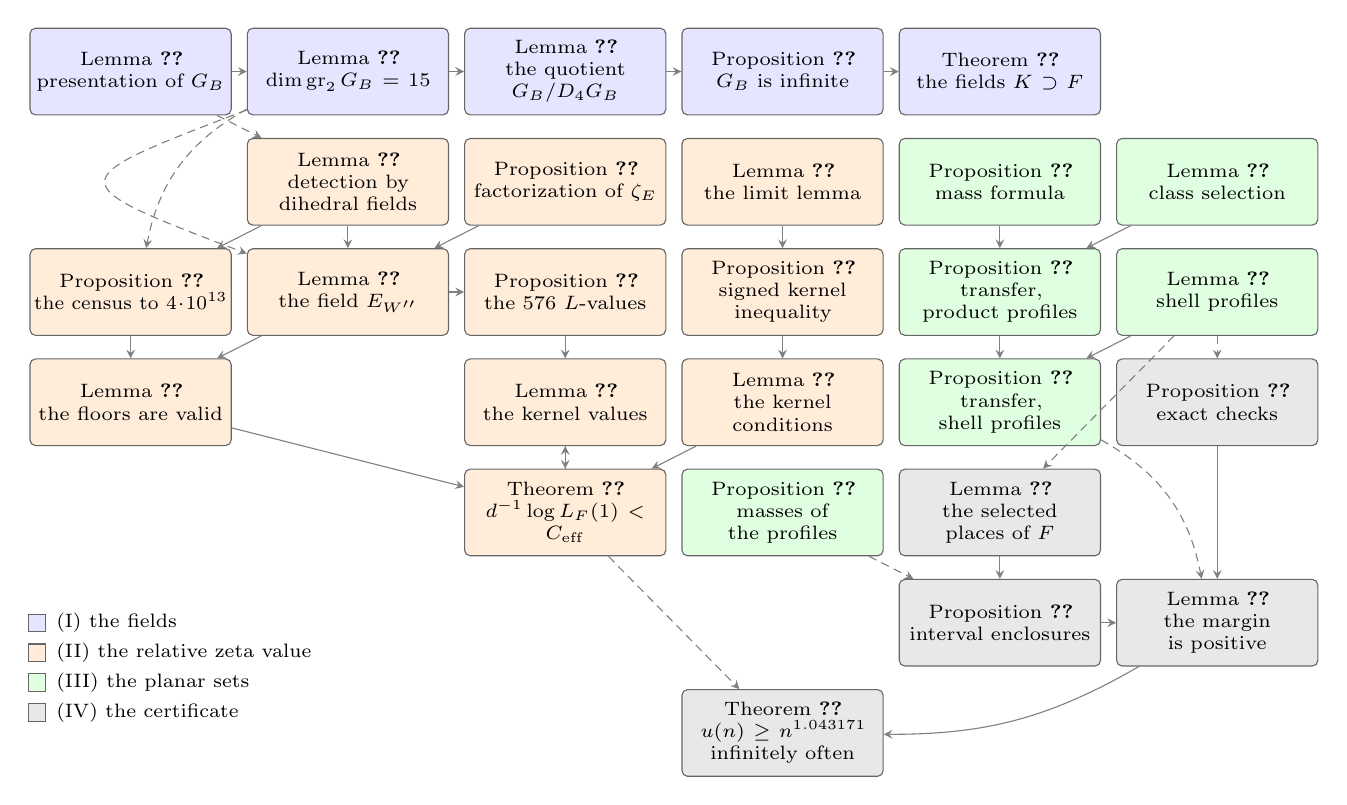
\begin{tikzpicture}[x=1cm,y=1cm,>=stealth,
 box/.style={draw=black!60,rounded corners=2pt,align=center,font=\scriptsize,
  execute at begin node={\hyphenpenalty=10000\exhyphenpenalty=10000},
  inner sep=1.5pt,minimum height=1.10cm,text width=2.45cm}]
\node[box,fill=blue!10] (tw-GB-presentation) at (0.000,0.000) {Lemma~\ref*{tw:GB-presentation}\\ presentation of $G_B$};
\node[box,fill=blue!10] (tw-quadratic-layer) at (2.760,0.000) {Lemma~\ref*{tw:quadratic-layer}\\ $\dim\operatorname{gr}_2G_B=15$};
\node[box,fill=blue!10] (tw-retained-quotient) at (5.520,0.000) {Lemma~\ref*{tw:retained-quotient}\\ the quotient $G_B/D_4G_B$};
\node[box,fill=blue!10] (tw-infinite) at (8.280,0.000) {Proposition~\ref*{tw:infinite}\\ $G_B$ is infinite};
\node[box,fill=blue!10] (tw-field-family) at (11.040,0.000) {Theorem~\ref*{tw:field-family}\\ the fields $K\supset F$};
\node[box,fill=orange!15] (dh-detection) at (2.760,-1.400) {Lemma~\ref*{dh:detection}\\ detection by dihedral fields};
\node[box,fill=orange!15] (gf-factorization) at (5.520,-1.400) {Proposition~\ref*{gf:factorization}\\ factorization of $\zeta_E$};
\node[box,fill=orange!15] (an-limit) at (8.280,-1.400) {Lemma~\ref*{an:limit}\\ the limit lemma};
\node[box,fill=orange!15] (dh-census) at (0.000,-2.800) {Proposition~\ref*{dh:census}\\ the census to $4\cdot10^{13}$};
\node[box,fill=orange!15] (dh-EW) at (2.760,-2.800) {Lemma~\ref*{dh:EW}\\ the field $E_{W''}$};
\node[box,fill=orange!15] (lv-values) at (5.520,-2.800) {Proposition~\ref*{lv:values}\\ the $576$ $L$-values};
\node[box,fill=orange!15] (an-signed) at (8.280,-2.800) {Proposition~\ref*{an:signed}\\ signed kernel inequality};
\node[box,fill=orange!15] (dh-floors-valid) at (0.000,-4.200) {Lemma~\ref*{dh:floors-valid}\\ the floors are valid};
\node[box,fill=orange!15] (ce-values) at (5.520,-4.200) {Lemma~\ref*{ce:values}\\ the kernel values};
\node[box,fill=orange!15] (ce-kernel) at (8.280,-4.200) {Lemma~\ref*{ce:kernel}\\ the kernel conditions};
\node[box,fill=orange!15] (an-ceiling) at (5.520,-5.600) {Theorem~\ref*{an:ceiling}\\ $d^{-1}\log L_F(1)<C_{\rm eff}$};
\node[box,fill=green!12] (geo-mass) at (11.040,-1.400) {Proposition~\ref*{geo:mass}\\ mass formula};
\node[box,fill=green!12] (geo-selection) at (13.800,-1.400) {Lemma~\ref*{geo:selection}\\ class selection};
\node[box,fill=green!12] (geo-transfer) at (11.040,-2.800) {Proposition~\ref*{geo:transfer}\\ transfer, product profiles};
\node[box,fill=green!12] (fw-shell-lemma) at (13.800,-2.800) {Lemma~\ref*{fw:shell-lemma}\\ shell profiles};
\node[box,fill=green!12] (fw-transfer) at (11.040,-4.200) {Proposition~\ref*{fw:transfer}\\ transfer, shell profiles};
\node[box,fill=green!12] (pf-mass) at (8.280,-5.600) {Proposition~\ref*{pf:mass}\\ masses of the profiles};
\node[box,fill=gray!18] (cert-exact) at (13.800,-4.200) {Proposition~\ref*{cert:exact}\\ exact checks};
\node[box,fill=gray!18] (cert-places) at (11.040,-5.600) {Lemma~\ref*{cert:places}\\ the selected places of $F$};
\node[box,fill=gray!18] (cert-enclosures) at (11.040,-7.000) {Proposition~\ref*{cert:enclosures}\\ interval enclosures};
\node[box,fill=gray!18] (cert-lower-margin) at (13.800,-7.000) {Lemma~\ref*{cert:lower-margin}\\ the margin is positive};
\node[box,fill=gray!18] (thm-main) at (8.280,-8.400) {Theorem~\ref*{thm:main}\\ $u(n)\ge n^{1.043171}$ infinitely often};
\draw[->,black!50] (an-ceiling) -- (ce-values);
\draw[->,black!50,densely dashed] (an-ceiling) -- (thm-main);
\draw[->,black!50] (an-limit) -- (an-signed);
\draw[->,black!50] (an-signed) -- (ce-kernel);
\draw[->,black!50] (ce-kernel) -- (an-ceiling);
\draw[->,black!50] (ce-values) -- (an-ceiling);
\draw[->,black!50] (cert-enclosures) -- (cert-lower-margin);
\draw[->,black!50] (cert-exact) -- (cert-lower-margin);
\draw[->,black!50] (cert-lower-margin) to[bend left=15] (thm-main);
\draw[->,black!50] (cert-places) -- (cert-enclosures);
\draw[->,black!50] (dh-EW) -- (dh-floors-valid);
\draw[->,black!50] (dh-EW) -- (lv-values);
\draw[->,black!50] (dh-census) -- (dh-floors-valid);
\draw[->,black!50] (dh-detection) -- (dh-EW);
\draw[->,black!50] (dh-detection) -- (dh-census);
\draw[->,black!50] (dh-floors-valid) -- (an-ceiling);
\draw[->,black!50,densely dashed] (fw-shell-lemma) -- (cert-exact);
\draw[->,black!50,densely dashed] (fw-shell-lemma) -- (cert-places);
\draw[->,black!50] (fw-shell-lemma) -- (fw-transfer);
\draw[->,black!50,densely dashed] (fw-transfer) to[bend left=25] (cert-lower-margin);
\draw[->,black!50] (geo-mass) -- (geo-transfer);
\draw[->,black!50] (geo-selection) -- (geo-transfer);
\draw[->,black!50] (geo-transfer) -- (fw-transfer);
\draw[->,black!50] (gf-factorization) -- (dh-EW);
\draw[->,black!50] (lv-values) -- (ce-values);
\draw[->,black!50,densely dashed] (pf-mass) -- (cert-enclosures);
\draw[->,black!50,densely dashed] (tw-GB-presentation) -- (dh-detection);
\draw[->,black!50] (tw-GB-presentation) -- (tw-quadratic-layer);
\draw[->,black!50] (tw-infinite) -- (tw-field-family);
\draw[->,black!50,densely dashed] (tw-quadratic-layer) .. controls (-0.920,-1.400) .. (dh-EW);
\draw[->,black!50,densely dashed] (tw-quadratic-layer) to[bend right=25] (dh-census);
\draw[->,black!50] (tw-quadratic-layer) -- (tw-retained-quotient);
\draw[->,black!50] (tw-retained-quotient) -- (tw-infinite);
\node[draw=black!60,fill=blue!10,minimum size=0.22cm,inner sep=0pt] at (-1.190,-7.000) {};
\node[anchor=west,font=\scriptsize,inner sep=0pt] at (-0.950,-7.000) {(I) the fields};
\node[draw=black!60,fill=orange!15,minimum size=0.22cm,inner sep=0pt] at (-1.190,-7.380) {};
\node[anchor=west,font=\scriptsize,inner sep=0pt] at (-0.950,-7.380) {(II) the relative zeta value};
\node[draw=black!60,fill=green!12,minimum size=0.22cm,inner sep=0pt] at (-1.190,-7.760) {};
\node[anchor=west,font=\scriptsize,inner sep=0pt] at (-0.950,-7.760) {(III) the planar sets};
\node[draw=black!60,fill=gray!18,minimum size=0.22cm,inner sep=0pt] at (-1.190,-8.140) {};
\node[anchor=west,font=\scriptsize,inner sep=0pt] at (-0.950,-8.140) {(IV) the certificate};
\end{tikzpicture}
\caption{The structure of the proof (Subsection~\ref{intro:structure}). Each box is a numbered statement, coloured by the part of the proof it belongs to. An arrow goes from a statement to each statement whose proof uses it, directly or through statements not shown, except that arrows implied by a chain of drawn arrows are left out; dashed arrows join different parts. The arrows from Theorem~\ref{tw:field-family}, which supplies the fields to which Parts (II)--(IV) apply, are also left out. Appendix~\ref{dep:section} lists the citations between all numbered statements; the notation is collected in Subsection~\ref{intro:notation}.}
\label{fig:structure}
\end{figure}

\subsection{The main ingredients}\label{intro:new}
\emph{The base field and the signature.} In the construction of Sawin
\cite{Sawin2026}, and in \cite{Naslund0358}, the field $K$ is a CM field:
$F$ is totally real, so $\theta=0$, and the norm-one units are finite.
Sawin's fields come from an unramified pro-$2$ tower over a real quadratic
field ramified at $2$ and at the thirteen odd primes up to $43$, and their
root discriminant is about $1.6\cdot10^8$. Here the base field is
$B=\Q(\sqrt{241})$, the real quadratic field of smallest discriminant in
which $2$, $3$ and $5$ all split. The tower is ramified only at the six
primes of $B$ above $2$, $3$ and $5$, with prescribed local Galois groups
there, and is still infinite (Proposition~\ref{tw:infinite}); its fields
have root discriminant $\lambda\approx286$. The field $K$ is totally
imaginary and Galois over $B$, and $F$ is the fixed field of one complex
conjugation, which is not central, so that almost every place of $F$ is
complex and $\theta\ge\theta_*$. Above a complex place of $F$ the two
coordinates of a norm-one element can have different moduli, and the
norm-one units, of rank $c$, move them along a lattice; averaging over a
fundamental domain of that lattice counts the resulting pairs exactly, and
the class-number formula cancels the regulator of these units
(Proposition~\ref{geo:mass}). By \eqref{intro:margin}, mixed signature adds
$\theta(J_\C-2J_\R-\log\pi)$ to the margin: with the profiles of
Section~\ref{sec:certificate}, the lower bound for the margin proved there
is positive for $\theta\ge\theta_*$, but would be below $-0.312$ at
$\theta=0$ (Remark~\ref{cert:signature-remark}).

\emph{The caps.} The local conditions of the tower bound the order of
the Frobenius elements by four (a \emph{cap}) at the two primes above
$29$ and at one of the two primes of $B$ above $41$ (the prime $41$ splits
in $B$). The capped primes are selected (Definition~\ref{an:selected-def}):
the primes of $F$ above them that split in $K$ are used for equal-norm
choices. A cap at the prime $7$, the smallest prime inert in $B$,
would cost the same in the Golod--Shafarevich function and would give the same
quotient $G_B/D_4G_B$ of the tower group, because every fourth power lies
in $D_4G_B$. But the selected primes above $41$ have residue field of
order $41^4$ instead of $7^8$, and their contribution to the margin is
about twice as large.

\emph{The relative zeta value.} The simplest bound for
$d^{-1}\log L_F(1)$, $C=\ceiling$ (Remark~\ref{an:base-ceiling}),
compares $\zeta_K$ prime by prime with the zeta function of the Kummer
field $E$, the maximal elementary abelian subextension of the tower,
with $[E:\Q]=512$. With this bound the construction gives the exponent
$1.042901$. A prime of $B$ that splits completely in $E$ is then
counted as if it split completely in $K$; such primes carry about $0.005$
of $C$. We recover most of this through the second graded piece
$\operatorname{gr}_2G_B=D_2G_B/D_3G_B$ of the Zassenhaus filtration, a
vector space over $\Ftwo$ of dimension $15$ (Lemma~\ref{tw:quadratic-layer}):
\begin{enumerate}
\item[(a)] Exactly $27$ linear forms on it are \emph{of dihedral type}
 (Definition~\ref{dh:dihedral-type}):
 they come from quotients of $G_B$ isomorphic to the dihedral group of
 order $8$, each realized by an explicit field of degree $8$ over $B$
 that lies in every field of the tower (Lemmas~\ref{dh:detection}
 and~\ref{dh:beta-exists}). Fifteen
 of them, with independent forms, detect the residue degree of every
 prime of degree one that splits completely in $E$ up to norm
 $4\cdot10^{13}$, except those whose Frobenius lies in $D_3G_B$
 (Subsection~\ref{dh:census-section}).
\item[(b)] The census cannot reach the infinite tail. Seven of the
 dihedral forms span a space $W''$ of dimension four
 (Subsection~\ref{dh:W-section}), and the corresponding field $\EW$, with
 $[\EW:\Q]=8192$, lies in every field of the tower
 (Subsection~\ref{dh:EW-section}). Its zeta function is
 the product of $\zeta_E$, of the squares of $448$ Hecke $L$-functions
 of quadratic characters of quartic fields, and of the fourth powers of
 $128$ Hecke $L$-functions of quadratic characters of octic fields
 (Lemmas~\ref{dh:EW} and~\ref{dh:Lfunctions}). Comparing with $\EW$ instead of $E$ moves fifteen
 sixteenths of the remaining primes, at all norms, from residue degree
 one to two. No larger space of this kind has $L$-functions of degree
 at most~$8$.
\item[(c)] We evaluate these $L$-functions rigorously at real points
 $\sigma$ near $1$, with approximate functional equations whose cut-off
 functions are certified for the four gamma factors that occur
 (Section~\ref{lv:section}); the octic $L$-functions have conductors up
 to $7.2\cdot10^{20}$ and need Dirichlet coefficients up to
 $1.06\cdot10^{11}$.
\item[(d)] The step from $\sigma>1$ to $s=1$ goes through the
 Tsfasman--Vl\u{a}du\c{t} inequality \cite[Proposition~3.1]{TsfasmanVladut2002}
 (Lemma~\ref{an:limit}(b)). Instead of one abscissa, we use a kernel
 $\mathsf K=\sum_jc_jg_{\sigma_j}$, where $g_\sigma(q)=-\log(1-q^{-\sigma})$,
 over $21$ abscissae $\sigma_j$ with coefficients $c_j$ of both signs;
 it dominates the prime-by-prime contribution at $s=1$ up to a multiple
 of the Tsfasman--Vl\u{a}du\c{t} weight
 $w(q)=2\log q\sum_{m\ge1}(q^m+1)^{-1}$ (Proposition~\ref{an:signed}).
\end{enumerate}
Together these lower the bound for $d^{-1}\log L_F(1)$ from $\ceiling$ to
$C_{\rm eff}=\Ceff$ (Theorem~\ref{an:ceiling}). Since the margin falls by
about $23.8$ per unit of $\delta$ and by $1$ per unit of $C$, this is
worth about $0.00027$ in the exponent.

\emph{General shell weights.} The shell profiles are weighted sums $\sum_{i,j}w_{ij}\mathbf 1_{\mathcal S_i\times
\varpi^{-k}\mathcal S_j}$ over products of \emph{shells}: in a local field
with ring of integers $\mathcal O$ and uniformizer $\varpi$,
$\mathcal S_0=\mathcal O$ and $\mathcal S_i$ ($i\ge1$) is the set of elements
of valuation $-i$, and $k$ is the exponent used at the prime
(Definition~\ref{fw:shell-profile}). Product weights $w_{ij}=x_ix_j$
suffice for the exponent $1.043170$; the local lemma allows any
nonnegative weights (Lemma~\ref{fw:shell-lemma}), and optimized symmetric
$10\times10$ matrices at the primes above $2$, $3$ and $5$ add
$1.5\cdot10^{-5}$ to the margin.

Table~\ref{intro:table-steps} shows the successive certified exponents.
Section~\ref{lim:section} describes the steps that are not needed for
Theorem~\ref{thm:main}, and what is known about the limits of the
method.

\begin{table}[htbp]
\centering\small
\caption{Successive exponents. $C_{\rm eff}$ is the bound for
$d^{-1}\log L_F(1)$ in force; each step keeps the previous ones, and the
profiles are re-optimized at each exponent. Rows marked $*$ are intermediate
certificates, described in Section~\ref{lim:section}; the proof of
Theorem~\ref{thm:main} uses the census, the signed kernel and the field
$\EW$, but not the adaptive dichotomy or the single-abscissa step. The row
marked $\dagger$ was computed during the search, with product shell weights,
and has no witness of its own; every other row has a witness
(Subsection~\ref{intro:code}) and a replay program in the repository.
$E_W$ and $E_{W'}$ are the fields of the spaces $W\subset W'\subset W''$ of
Section~\ref{lim:section}, and ``ceiling over $M$'' means the bound for
$d^{-1}\log L_F(1)$ obtained with $M$ as comparison field.}
\label{intro:table-steps}
\begin{tabular}{@{}p{8.6cm}lr@{}}
\toprule
step & $C_{\rm eff}$ & exponent\\
\midrule
caps above $29$ and $41$, comparison field $E$ & $0.04871285$ & $1.042901$\\
${}^*$adaptive dichotomy (Propositions~\ref{lim:A}, \ref{lim:B}) & $0.048134265$ & $1.042925$\\
${}^*$dihedral census to $10^{12}$ & $0.0471692613$ & $1.042965$\\
${}^*$ceiling over $E_W$, $[E_W:\Q]=2048$, census to $10^{13}$ & $0.0436495$ & $1.043113$\\
${}^*$refined Tsfasman--Vl\u{a}du\c{t} step, one abscissa & $0.0435763$ & $1.043116$\\
${}^*$signed kernel, census to $8.5\cdot10^{14}$ & $0.0433891$ & $1.043124$\\
${}^*$ceiling over $E_{W'}$, $[E_{W'}:\Q]=4096$ & $0.0427163$ & $1.043152$\\
${}^\dagger$ceiling over $\EW$, $[\EW:\Q]=8192$, census to $4\cdot10^{13}$ & $0.0422764$ & $1.043170$\\
general shell weights at $2$, $3$, $5$ & $0.0422764$ & $1.043171$\\
\bottomrule
\end{tabular}
\end{table}

\subsection{Status}\label{intro:status}
The proof of Theorem~\ref{thm:main} is complete as written, but parts of
it rest on computations. Each computation is done by a supplementary
program, named where it is used, in exact arithmetic or in outward-rounded
interval arithmetic, and a replay program reruns the certificate
(Subsection~\ref{intro:code}). The dihedral refinements, the signed
kernel, the general shell weights and the intermediate certificates were
checked by ten independent reviews by AI agents in fresh contexts, each
given the statements, the arguments and the programs but not the author's
confidence or earlier verdicts. One review
found a material error in an intermediate certificate: thirteen primes
had been credited twice. It was corrected; the exponent of that step did
not change. The other reviews found no error affecting the bounds; their
minor points, among them gaps in the error accounting of the numerical
programs, were fixed. No reviewer recomputed the octic $L$-values
independently, since general-purpose software cannot reach their
conductors; they rest on the method of Section~\ref{lv:section} and its
checks. The cap above $41$ (Section~\ref{tw:tower}) has had two
fresh-context reviews of its argument, but its finite computations have
not had a full independent review. The manuscript as a whole had three
further fresh-context reviews, which found no error affecting the theorem
or any constant, and an audit of the floating-point arithmetic of the
$L$-value programs found every bound rigorous. These are
automated reviews, not human peer review.

A Lean formalization \cite{NaslundLeanW} of the tower of the present
paper proves the planar conclusion with the exponent $1.04315$ from one
explicit inequality for $\zeta_{\EW}$ (Remark~\ref{an:lean-hypothesis}).
The inequality is not proved in Lean, and the formalization does not cover
the census beyond norm $1000$, the signed kernel or the general shell
weights, so it does not prove Theorem~\fref{thm:main}, even
conditionally.

\subsection{Organization}\label{intro:organization}
Section~\ref{tw:tower} constructs the tower and proves
Theorem~\ref{tw:field-family}, which supplies the fields.
Section~\ref{gf:section} describes the Kummer field $E$ and its quadratic
$L$-functions. Section~\ref{an:section} reduces the relative zeta value
to the primes of the fields of the tower, and proves the signed kernel
inequality (Proposition~\ref{an:signed}). Section~\ref{dh:section} treats
the dihedral quotients, the census and the field $\EW$;
Section~\ref{lv:section} evaluates the $L$-functions of $\EW$; and
Section~\ref{ce:section} proves the bound $C_{\rm eff}$
(Theorem~\ref{an:ceiling}). Sections~\ref{geo:section}--\ref{pf:section}
carry out the geometric construction, with
general shell weights. Section~\ref{sec:certificate} proves the final
inequality at $\delta=\deltastar$ and completes the proof of
Theorem~\ref{thm:main}. Section~\ref{lim:section} records refinements that
are not used, and the limits of the method. Appendix~\ref{fw-data:section}
lists the optimized shell weights, and the dependency index
(Appendix~\ref{dep:section}) lists, for every numbered statement, the
statements it cites and those that cite it.

\subsection{Notation}\label{intro:notation}
The following symbols keep one meaning throughout the paper. Other letters
($H$, $N$, $\tau$, $\beta$, $\gamma$, $\sigma$, $\nu$, $q$, $s$, $t$, \dots)
are reused in different sections with local meanings, which are defined
where they are introduced.

\smallskip
{\small
\begin{longtable}{@{}>{\raggedright\arraybackslash}p{0.2\textwidth}>{\raggedright\arraybackslash}p{0.53\textwidth}>{\raggedright\arraybackslash}p{0.21\textwidth}@{}}
\toprule
symbol & meaning & defined in\\
\midrule\endhead
$B$, $S$ & $B=\Q(\sqrt{241})$; $S$ the primes of $B$ above $2,3,5$ & Section~\ref{tw:tower}\\
$\mathrm N$ & the absolute norm of an ideal & Section~\ref{tw:tower}\\
$\mathfrak t_1,\dots,\mathfrak t_4$ & the primes of $B$ above $29$ and $41$; the capped primes are $\mathfrak t_1,\mathfrak t_2,\mathfrak t_3$ & Lemma~\ref{tw:base}, Definition~\ref{tw:local-generators}\\
$v_1,v_2$, $\Sigma$ & the real places of $B$; $\Sigma=S\cup\{v_1,v_2\}$ & Section~\ref{tw:tower}\\
$B_S$, $G_S$ & the maximal pro-$2$ extension of $B$ unramified at the finite primes outside $S$, and its Galois group & Section~\ref{tw:tower}\\
$E$ & the Kummer field: the maximal elementary abelian $2$-extension of $B$ in $B_S$, $[E:\Q]=512$ & Section~\ref{tw:tower}\\
$\chi_e$, $\kappa_a$ & the characters of $\Gal(E/B)$, with values $\pm1$ and in $\Ftwo$ & Definitions~\ref{gf:characters}, \ref{tw:elementary-image}\\
$D_nG$, $\operatorname{gr}_nG$ & the Zassenhaus filtration of a pro-$2$ group $G$ and its graded pieces $D_nG/D_{n+1}G$ & Section~\ref{tw:tower}\\
$G_B$, $B_G$, $\overline G_B$ & the tower group; the field $B_G\subset B_S$ of the tower, with $\Gal(B_G/B)=G_B$; and $\overline G_B=G_B/D_4G_B$ & Definition~\ref{tw:GB}\\
$\iota_1$ & a complex conjugation at a place above $v_1$ & Definition~\ref{tw:local-generators}\\
$\rd(M)$, $\lambda$, $\ell$ & root discriminant; $\lambda=2^{9/4}\sqrt{3615}$, the root discriminant of the fields of the tower; $\ell=\log\lambda$ & Definition~\ref{tw:rd}, Theorem~\ref{tw:field-family}\\
$\mathcal K$, $K$, $F$, $d$ & the fields of the tower used; $K\in\mathcal K$, $F=K^{\langle\iota_1\rangle}$, $d=[F:\Q]$ & Definition~\ref{an:family}\\
$(b,c)$, $\theta$, $\theta_*$ & the signature of $F$ ($d=b+2c$), $\theta=c/d$, and the lower bound $\theta_*=\thetastar$ & Theorem~\ref{tw:field-family}\\
$L_F(s)$ & the relative zeta function $\zeta_K(s)/\zeta_F(s)$ & Subsection~\ref{intro:outline}\\
$C$, $C_{\rm eff}$ & an upper bound for $d^{-1}\log L_F(1)$; the bound $C_{\rm eff}=\Ceff$ proved here & Theorem~\ref{an:ceiling}\\
$e_K(\mathfrak p)$, $f_K(\mathfrak p)$ & ramification index and residue degree of a prime $\mathfrak p$ of $B$ in $K/B$ & Section~\ref{an:section}\\
$g_s(q)$, $w(q)$, $\kappa_\infty$ & $g_s(q)=-\log(1-q^{-s})$; $w(q)$ the Tsfasman--Vl\u{a}du\c{t} weight, and $2\kappa_\infty$ the right side of the Tsfasman--Vl\u{a}du\c{t} inequality & Subsection~\ref{an:budget-section}\\
$\beta_q$, $Z(s)$ & limiting densities of primes of norm $q$, and $Z(s)=\sum_q\beta_qg_s(q)$ & Lemma~\ref{an:limit}\\
$Z_{\rm sel}$, $T_{\rm sel}$ & the parts of $Z$ and of the Tsfasman--Vl\u{a}du\c{t} sum from the selected primes & Subsection~\ref{an:selected}\\
selected, free & the selected primes of $B$ (above $2,3,5$ and the capped primes); the other primes of $B$ & Definition~\ref{an:selected-def}\\
$f^0_{\mathfrak p}$, $Y_{\rm fl}$ & floors: lower bounds for the residue degrees of the free primes, conditions (Fl1), (Fl2); the floor sum & Definition~\ref{an:floor-def}\\
$\mathsf K$, $\sigma_j$, $c_j$, $b_{\rm TV}$ & the signed kernel $\sum_jc_jg_{\sigma_j}$ with its $21$ abscissae and coefficients, and its multiplier of $w$ & Proposition~\ref{an:signed}, Definition~\ref{ce:kernel-def}\\
$\mathrm{Dih}_4$, $\psi_o$ & the dihedral group of order $8$; the $27$ forms of dihedral type on $\operatorname{gr}_2G_B$ & Definition~\ref{dh:dihedral-type}, Lemma~\ref{dh:27}\\
$\psi^{\rm c}_1,\dots,\psi^{\rm c}_{15}$ & the census basis of dihedral forms & Definition~\ref{dh:census-basis}\\
$W''$, $\EW$ & the span of seven dihedral forms, $\dim W''=4$, and its field, $[\EW:\Q]=8192$ & Definition~\ref{dh:W}\\
$\delta$, $p$ & the exponent is $1+\delta$; $p=2/(1+\delta)$ is a Lebesgue exponent & Definition~\ref{geo:profiles}\\
$\mathcal S_i$, $\mathcal F_{\delta,\mathfrak p}$ & the shells of a local field; the local functional of the shell profile at $\mathfrak p$ & Definitions~\ref{fw:local-functional}, \ref{fw:shell-profile}\\
$J_\R$, $J_\C$ & the archimedean functionals of the profiles & Definition~\ref{geo:profiles}\\
$(e_r,f_r)$ & for $r=2,3,5,29$ the type of the selected places above $r$; for $r=41$ the
 \emph{effective type} $(2,4)$, a counting device & Definition~\ref{cert:effective-types}\\
\bottomrule
\end{longtable}}

\subsection{Computations and data}\label{intro:code}
The proof uses finite computations: linear algebra over $\Ftwo$ for the
tower and its quotients, exact rational arithmetic for the
Golod--Shafarevich function, a census of primes in C, rigorous
evaluations of $L$-functions in the ball arithmetic of Arb, now part of
FLINT \cite{Johansson2017,FLINT}, and interval arithmetic with directed
rounding for the margin \cite{Mpmath}. PARI/GP \cite{PARI} is used for
the arithmetic of number fields and for independent checks. Each finite
fact is verified by a supplementary program, named in the text where the
fact is used.

The programs and their data are in the directory
\path{papers/0.043171/certificates} of the repository
\cite{NaslundCode4317}. They import, without modifying them, programs
in the directories \path{papers/0.04273/certificates} and
\path{papers/0.042901/certificates} of the same repository (the
arithmetic of $B$ and of $E$, the analytic ceiling with $E$ as comparison
field, and the geometric margin) and some routines of the data archive in
\path{papers/0.0418235/certificates}, whose members are checked against
their SHA-256 hashes when the archive is unpacked. A \emph{witness} is a JSON file that
records the exact data of one certificate (the exponent, the bound $C$,
the kernel abscissae and coefficients, the profile parameters and the
shell weights) together with the SHA-256 hashes of the data files it
reads; its replay program recomputes every certified inequality from it.
The witness of Theorem~\ref{thm:main} is
\path{certificates/dihedral/witness_0.043171.json}; it pins the
SHA-256 hashes of $683$ data files, among them all $356$ files that the
certification reads.
The replay program \path{certificates/dihedral/reproduce_w3.py}
regenerates the exports of the number fields with PARI/GP, recomputes
the $L$-values at three of the abscissae and checks the others by hash,
repeats the census on sample ranges and checks the census bins against
an independent classification, reruns the kernel checks and the bound
for the relative zeta value, and recomputes the margin. It takes about
two hours on a machine with sixteen cores. The computations were run
with PARI/GP~2.17.2, python-flint~0.9.0 (FLINT~3.6.0), mpmath~1.3.0,
numpy~2.5.3 and scipy~1.18.1; the census programs need an x86-64
processor with the AVX-512 IFMA instructions.
\tableofcontents
\section{\texorpdfstring{The Tower over $\Q(\sqrt{241})$}{The Tower over Q(sqrt 241)}}\label{tw:tower}

This section constructs the number fields of Theorem~\ref{tw:field-family}
as finite subextensions of an infinite pro-$2$ extension of $B=\Q(\sqrt{241})$
with prescribed local Galois groups: ramification is allowed only above
$2$, $3$ and $5$, and the order of the Frobenius is bounded by four at the
two primes $\mathfrak t_1,\mathfrak t_2$ above $29$ and at one of the two
primes $\mathfrak t_3,\mathfrak t_4$ above $41$, namely $\mathfrak t_3$
(Lemma~\ref{tw:base}). Subsection~\ref{tw:base-section} describes $B$ and its
$\{2,3,5\}$-units. Subsection~\ref{tw:local-section} recalls the local Galois
groups involved and constructs the dyadic local field.
Subsection~\ref{tw:global-section} shows that the Galois group
$G_S$ of the maximal pro-$2$ extension of $B$ unramified outside
$2,3,5$ has a presentation with eight generators and seven local relators
(Lemma~\ref{tw:complete-global-presentation}).
Subsection~\ref{tw:prescribed-section} imposes the local conditions and
defines the quotient $G_B$ of $G_S$ (Definition~\ref{tw:GB}).
Subsection~\ref{tw:retained-section} computes the first three graded pieces
of the Zassenhaus filtration $(D_nG_B)_n$ of $G_B$, recalled below: the
prescribed local groups inject into $G_B/D_3G_B$, and the complex
conjugation $\iota_1$ (Definition~\ref{tw:local-generators}) has $2^{15}$
conjugates in $G_B/D_4G_B$ (Lemma~\ref{tw:retained-quotient}).
Subsections~\ref{tw:fox-section} and~\ref{tw:infinite-section} prove that
$G_B$ is infinite, by a filtered Fox calculus and the Golod--Shafarevich
method \cite{GolodShafarevich}: the Golod--Shafarevich function $P_B$ of
\eqref{tw:PB} takes a negative value (Lemma~\ref{tw:PB-value}).
Subsection~\ref{tw:fields-section} proves Theorem~\ref{tw:field-family}.
Later sections use Theorem~\ref{tw:field-family} (the fields, their root
discriminant, signature and local types), the elementary images of
Table~\ref{tw:vector-table} (Section~\ref{gf:section} and the census of
Section~\ref{an:section}), and the description
$\operatorname{gr}_2G_B=\mathfrak L_2/R_2$ of Lemmas~\ref{tw:graded}
and~\ref{tw:quadratic-layer} (Sections~\ref{an:section}
and~\ref{dh:section}).

We use the following conventions. Subgroups of profinite groups are closed,
generation is topological, and the normal closure of a set is the smallest
closed normal subgroup containing it. The commutator is
$[g,h]=g^{-1}h^{-1}gh$. The \emph{generator rank} and the \emph{relation
rank} of a pro-$2$ group $G$ are $\dim H^1(G,\Ftwo)$ and $\dim H^2(G,\Ftwo)$.
For an extension $M/A$ of local or global fields, $\mathfrak D_{M/A}$ denotes
its different and $\mathfrak d_{M/A}$ its relative discriminant. For a finite
$2$-group $\Delta$ with augmentation
ideal $\mathfrak I\subset\Ftwo[\Delta]$, the Zassenhaus filtration is
$D_n\Delta=\{g:g-1\in\mathfrak I^n\}$; for a pro-$2$ group it is defined
through finite quotients. Then $[D_m,D_n]\subset D_{m+n}$, $g^2\in D_{2n}$
for $g\in D_n$, a surjection maps $D_n$ onto $D_n$, and
$\operatorname{gr}\Delta=\bigoplus_{n\ge1}\operatorname{gr}_n\Delta$, with
graded pieces $\operatorname{gr}_n\Delta=D_n\Delta/D_{n+1}\Delta$, is a
restricted Lie algebra over $\Ftwo$ whose bracket is induced by commutators
and whose restricted square $v\mapsto v^{[2]}$ is induced by squaring
\cite{Jennings,Quillen,Ershov2012}. By Lazard's formula
\cite[Proposition~3.2]{Ershov2012}, $D_n=\prod_{i2^j\ge n}\gamma_i^{2^j}$,
where $\gamma_i$ is the lower central series. In particular $D_1$ is the
whole group, $D_2$ is the Frattini subgroup, and $D_3=D_2^{\,2}[D_2,D_1]$. For
a free pro-$2$ group $\mathfrak F$ of rank $n$ (free pro-$2$ groups are
written in fraktur: $\mathfrak F$, $\mathfrak F_k$, $\mathfrak F'$),
$\operatorname{gr}\mathfrak F$ is the free restricted Lie algebra on $\mathfrak F/D_2\mathfrak F\cong\Ftwo^n$
\cite{Quillen,Ershov2012}. We realize it inside the free associative
algebra $\Ftwo\langle X_1,\dots,X_n\rangle$, with bracket $[a,b]=ab+ba$ and
restricted square $a^{[2]}=a^2$; its graded pieces of degrees one, two and
three have dimensions $n$, $n(n+1)/2$ and $(n^3-n)/3$.

\begin{definition}\label{tw:hilbert-def}
A \emph{filtered space} is a finite-dimensional $\Ftwo$-vector space $M$
with subspaces
$M=\operatorname{Fil}^0M\supseteq\operatorname{Fil}^1M\supseteq\cdots$ such
that $\operatorname{Fil}^mM=0$ for large $m$. Its \emph{Hilbert polynomial}
is
$h_M(t)=\sum_{m\ge0}\dim(\operatorname{Fil}^mM/\operatorname{Fil}^{m+1}M)\,t^m$.
For a finite $2$-group $\Delta$ we filter $\Ftwo[\Delta]$ by the powers
$\mathfrak I^m$ of its augmentation ideal $\mathfrak I$, so that
$h_{\Ftwo[\Delta]}(t)=\sum_{m\ge0}\dim(\mathfrak I^m/\mathfrak I^{m+1})\,t^m$.
\end{definition}

\begin{theorem}[Jennings \cite{Jennings}; see also \cite{Quillen}]\label{tw:jennings}
Let $\Delta$ be a finite $2$-group, and let $g_1,\dots,g_m\in\Delta$ be
elements whose classes form a basis of $\operatorname{gr}\Delta$ consisting of
homogeneous elements, the class of $g_i$ lying in
$\operatorname{gr}_{n_i}\Delta$. Then the products
$(g_1-1)^{a_1}\cdots(g_m-1)^{a_m}$ with $a_i\in\{0,1\}$, taken in this order,
form a basis of $\Ftwo[\Delta]$, and those with $\sum_ia_in_i\ge n$ form a
basis of $\mathfrak I^n$. The same holds with the factors taken in any other
fixed order (Remark~\fref{tw:jennings-order}). Consequently
\[
 h_{\Ftwo[\Delta]}(t)=\prod_{n\ge1}(1+t^n)^{\dim\operatorname{gr}_n\Delta}.
\]
\end{theorem}

\begin{remark}\label{tw:jennings-order}
The form of Theorem~\ref{tw:jennings} with the factors in an arbitrary fixed
order follows from Quillen's description of $\operatorname{gr}\Ftwo[\Delta]$
as the restricted enveloping algebra of $\operatorname{gr}\Delta$
\cite{Quillen} and the restricted Poincar\'e--Birkhoff--Witt theorem. We use
this freedom in Lemma~\ref{tw:filtered-local-freeness}(a), where the elements
of a subgroup are placed last.
\end{remark}

\subsection{The Base Field}\label{tw:base-section}
This subsection fixes the $\{2,3,5\}$-units $\alpha_0,\dots,\alpha_7$ of
$B$, the primes above $2,3,5,29,41$ and their square classes
(Lemma~\ref{tw:base}, Table~\ref{tw:squareclass-table}); every later
Kummer-theoretic computation reads off these data.

Let $B=\Q(\sqrt{241})$, with real places $v_1$ ($\sqrt{241}\mapsto+\sqrt{241}$)
and $v_2$ ($\sqrt{241}\mapsto-\sqrt{241}$). Put
\begin{equation}\label{tw:alpha}
\begin{gathered}
 \alpha_0=-1,\qquad \alpha_1=\varepsilon=-71011068+4574225\sqrt{241},\\
 \alpha_2=\tfrac{-6101-393\sqrt{241}}2,\qquad
 \alpha_3=\tfrac{6101-393\sqrt{241}}2,\\
 \alpha_4=31-2\sqrt{241},\quad \alpha_5=31+2\sqrt{241},\quad
 \alpha_6=326-21\sqrt{241},\quad \alpha_7=326+21\sqrt{241}.
\end{gathered}
\end{equation}
Their norms $\mathrm N_{B/\Q}(\alpha_i)$ are $1,-1,-2,-2,-3,-3,-5,-5$, and
$\alpha_2\alpha_3=2$, $\alpha_4\alpha_5=-3$, $\alpha_6\alpha_7=-5$. For a
nonzero ideal $\mathfrak a$ of $\mathcal O_B$ we write
$\mathrm N\mathfrak a=|\mathcal O_B/\mathfrak a|$ for its absolute norm.

\begin{lemma}\label{tw:base}
\begin{enumerate}
\item[(a)] $\mathcal O_B=\Z[(1+\sqrt{241})/2]$, the discriminant of $B$ is
 $241$, and $B$ has class number one.
\item[(b)] The unit $\varepsilon$ has norm $\mathrm N_{B/\Q}(\varepsilon)=-1$, and the
 classes of $-1$ and $\varepsilon$ form a basis of
 $\mathcal O_B^\times/\mathcal O_B^{\times2}$.
\item[(c)] In $\mathcal O_B$ we have $2=\mathfrak p_1\mathfrak p_2$,
 $3=\mathfrak q_1\mathfrak q_2$, $5=\mathfrak r_1\mathfrak r_2$ and
 $29=\mathfrak t_1\mathfrak t_2$, where
 \[
  \mathfrak p_j=\alpha_{1+j}\mathcal O_B,\quad
  \mathfrak q_j=\alpha_{3+j}\mathcal O_B,\quad
  \mathfrak r_j=\alpha_{5+j}\mathcal O_B,\quad
  \mathfrak t_j=(-14127\pm910\sqrt{241})\mathcal O_B,
 \]
 with the sign $+$ for $j=1$. These eight primes are distinct and of degree
 one. Likewise $41=\mathfrak t_3\mathfrak t_4$ with
 $\mathfrak t_3=(621+40\sqrt{241})\mathcal O_B$ and
 $\mathfrak t_4=(621-40\sqrt{241})\mathcal O_B$, two distinct primes of degree
 one. The prime $7$ is inert, and we write $\mathfrak t_0=7\mathcal O_B$, so
 that $\mathrm N\mathfrak t_0=49$. The prime $241$ ramifies. At each of the ten
 primes of degree one above $p\in\{2,3,5,29,41\}$ listed here, the completion
 of $B$ is $\Q_p$, and $\sqrt{241}$ maps to the square root of $241$ in $\Z_p$
 given in Table~\ref{tw:squareclass-table}.
\item[(d)] Let $S=\{\mathfrak p_1,\mathfrak p_2,\mathfrak q_1,\mathfrak q_2,\mathfrak r_1,\mathfrak r_2\}$
 and $V=\mathcal O_B[1/30]^\times/\mathcal O_B[1/30]^{\times2}$. The classes
 of $\alpha_0,\dots,\alpha_7$ form a basis of $V$, and $V$ is the subgroup of
 $B^\times/B^{\times2}$ of classes with even valuation at every prime outside
 $S$. Moreover $\Pic(\mathcal O_B[1/30])=0$.
\item[(e)] The element $\alpha_i$ is a square modulo $\mathfrak t_3$ exactly
 for $i=0,1,5,6,7$, and modulo $\mathfrak t_4$ exactly for $i=0,1,4,6,7$.
 The residue field of $\mathfrak t_0$ is $\mathbb F_{49}$, and $\alpha_i$ is a
 square modulo $\mathfrak t_0$ exactly for $i=0,4,5,6,7$.
\end{enumerate}
\end{lemma}

\begin{proof}
(a) Since $241\equiv1\pmod 4$, the ring of integers and the discriminant are
as stated. The Minkowski bound is $\sqrt{241}/2<8$, so every ideal class
contains an integral ideal of norm at most $7$, which is a product of primes
of norm at most $7$. By (c), these are the six primes above $2,3,5$, and they
are principal.

(b) A direct computation gives $71011068^2-241\cdot4574225^2=-1$. By
Dirichlet's theorem $\mathcal O_B^\times=\{\pm1\}\times\eta^{\Z}$ for a
fundamental unit $\eta$, and $\varepsilon=\pm\eta^k$. Since
$\mathrm N_{B/\Q}(\varepsilon)=-1$, the exponent $k$ is odd, so $-1$ and
$\varepsilon$ generate $\mathcal O_B^\times$ modulo squares. Neither $-1$ nor
$\pm\varepsilon$ is a square, because $B$ is real and
$\mathrm N_{B/\Q}(\pm\varepsilon)=-1$.

(c) We have $241\equiv1\pmod8$, $241\equiv1\pmod3$, $241\equiv1\pmod5$,
$241\equiv9\pmod{29}$, $241\equiv36\pmod{41}$ and $241\equiv3\pmod7$, and $3$
is not a square modulo $7$. Hence $2,3,5,29,41$ split, $7$ is inert and $241$
ramifies. The listed generators have norms $\pm2,\pm3,\pm5,29,41$ (for
instance $621^2-241\cdot40^2=41$), so they generate primes of degree one, and
the displayed products show that the two generators above each $p$ generate
the two distinct primes above $p$; for $29$ and $41$ the product of the two
generators is $p$. A prime of degree one above $p$ is the preimage of
$p\Z_p$ under an embedding $B\to\Q_p$, which sends $\sqrt{241}$ to one of
the two square roots of $241$ in $\Z_p$; the completion there is $\Q_p$, and
the prime contains the stated generator exactly for the square root in
Table~\ref{tw:squareclass-table}.

(d) Every $S$-unit $u$ satisfies
$u\mathcal O_B=\prod_{i\ge2}(\alpha_i\mathcal O_B)^{a_i}$, so
$u\prod_{i\ge2}\alpha_i^{-a_i}$ is a unit, and by (b) the classes of
$\alpha_0,\dots,\alpha_7$ generate $V$. If $\prod_i\alpha_i^{a_i}$ with
$a_i\in\{0,1\}$ is a square, the valuations at $S$ give $a_i=0$ for $i\ge2$,
and then (b) gives $a_0=a_1=0$. If $b\in B^\times$ has even valuation outside
$S$, then
$b\mathcal O_B=\mathfrak a^2\prod_{\mathfrak p\in S}\mathfrak p^{a_{\mathfrak p}}$
with $\mathfrak a$ principal by (a), so $b$ is an $S$-unit times a square.
Finally $\Pic(\mathcal O_B[1/30])$ is a quotient of $\Pic(\mathcal O_B)=0$.

(e) At $\mathfrak t_3$ and $\mathfrak t_4$ the residue field is $\mathbb F_{41}$
and $\sqrt{241}\mapsto6$, respectively $35$, since $621+40\cdot6=21\cdot41$
and $621-40\cdot35=-19\cdot41$; the statement is a computation of Legendre
symbols modulo $41$, repeated by the supplementary programs
\texttt{kummer41.gp} and \texttt{check41.py}. By (c), $\mathrm N\mathfrak t_0=49$. An
element $a\in\mathcal O_B$ prime to
$\mathfrak t_0$ is a square modulo $\mathfrak t_0$ exactly when
$a^{24}\equiv1$, that is, when the reduction of $\mathrm N_{B/\Q}(a)\equiv a^8$ is a
square in $\mathbb F_7$. By the norms listed after \eqref{tw:alpha}, this
holds for $\alpha_i$ exactly when $i=0,4,5,6,7$.
\end{proof}

\begin{table}[htbp]
\centering
\caption{The image of $\sqrt{241}$ in $\Z_p$ at each prime of degree one,
given by its residue, and in $\R$ at the real places; the classes of
$\alpha_0,\dots,\alpha_7$ in $\Q_p^\times/\Q_p^{\times2}$ at these primes, and
their signs at the real places. At $p=2$ the classes are written as
$\pm1,\pm5,\pm2,\pm10$; at odd $p$ as $1,u,p,up$, where $u=-1,2,2,3$ is a
nonsquare unit for $p=3,5,29,41$.}
\label{tw:squareclass-table}
\begin{tabular}{llrrrrrrrr}
\toprule
place & $\sqrt{241}\mapsto$ & $\alpha_0$ & $\alpha_1$ & $\alpha_2$ & $\alpha_3$ & $\alpha_4$ & $\alpha_5$ & $\alpha_6$ & $\alpha_7$\\
\midrule
$\mathfrak p_1$ & $7\bmod 32$ & $-1$ & $-5$ & $-10$ & $-5$ & $1$ & $5$ & $-5$ & $1$\\
$\mathfrak p_2$ & $25\bmod 32$ & $-1$ & $5$ & $5$ & $10$ & $5$ & $1$ & $1$ & $-5$\\
$\mathfrak q_1$ & $2\bmod 3$ & $-1$ & $1$ & $-1$ & $1$ & $3$ & $-1$ & $-1$ & $-1$\\
$\mathfrak q_2$ & $1\bmod 3$ & $-1$ & $-1$ & $-1$ & $1$ & $-1$ & $3$ & $-1$ & $-1$\\
$\mathfrak r_1$ & $1\bmod 5$ & $1$ & $2$ & $2$ & $1$ & $1$ & $2$ & $10$ & $2$\\
$\mathfrak r_2$ & $4\bmod 5$ & $1$ & $2$ & $1$ & $2$ & $2$ & $1$ & $2$ & $10$\\
$\mathfrak t_1$ & $3\bmod 29$ & $1$ & $1$ & $2$ & $1$ & $1$ & $2$ & $2$ & $2$\\
$\mathfrak t_2$ & $26\bmod 29$ & $1$ & $1$ & $1$ & $2$ & $2$ & $1$ & $2$ & $2$\\
$\mathfrak t_3$ & $6\bmod 41$ & $1$ & $1$ & $3$ & $3$ & $3$ & $1$ & $1$ & $1$\\
$\mathfrak t_4$ & $35\bmod 41$ & $1$ & $1$ & $3$ & $3$ & $1$ & $3$ & $1$ & $1$\\
$v_1$ & $+\sqrt{241}$ & $-$ & $+$ & $-$ & $-$ & $-$ & $+$ & $-$ & $+$\\
$v_2$ & $-\sqrt{241}$ & $-$ & $-$ & $+$ & $+$ & $+$ & $-$ & $+$ & $-$\\
\bottomrule
\end{tabular}
\end{table}

The classes in Table~\ref{tw:squareclass-table} follow from the residues of
$\sqrt{241}$ given there; at $p=2$ they need its image modulo $32$. For
example, at $\mathfrak p_1$ we have $4574225\equiv1$ and $-71011068\equiv4$
modulo $8$, so $\varepsilon\equiv4+7\equiv3\equiv-5\pmod 8$. The classes
modulo the inert prime $\mathfrak t_0$ are given by Lemma~\ref{tw:base}(e);
the prime $\mathfrak t_0$ carries no condition in this paper.

\subsection{Local Galois Groups}\label{tw:local-section}
This subsection gives presentations of the local pro-$2$ Galois groups, with
the quadratic initials of their relators (Lemma~\ref{tw:local-groups}), and
constructs the dyadic local field $L_2$ with Galois group $\mathcal D$
(Lemma~\ref{tw:local-two}). These are the local conditions of the tower and
the local inputs of the Golod--Shafarevich estimate of
Subsections~\ref{tw:fox-section} and~\ref{tw:infinite-section}.

For a prime $p$ let $\mathcal G_{\Q_p}$ be the Galois group of the maximal
pro-$2$ extension of $\Q_p$, and for a place $\nu$ of $B$ let $\mathcal G_\nu$
be the Galois group of the maximal pro-$2$ extension of the completion
$B_\nu$; for a real place, $\mathcal G_\nu=\Gal(\C/\R)$. We write
$(\cdot,\cdot)$ for the Hilbert symbol
of order two of a local field \cite[Chapter~III, Section~4]{MilneCFT}. For
odd $p$ and $p$-adic units $u,w$, and for $2$-adic units $u,w$,
\begin{equation}\label{tw:hilbert}
 (p^au,p^bw)_p=(-1)^{ab(p-1)/2}\Bigl(\frac up\Bigr)^b\Bigl(\frac wp\Bigr)^a,
 \qquad
 (2^au,2^bw)_2=(-1)^{\frac{u-1}2\frac{w-1}2+a\frac{w^2-1}8+b\frac{u^2-1}8}
\end{equation}
\cite[Chapter~III, Theorem~1]{SerreCourse}, \cite[Chapter~VIII,
Section~5]{MilneCFT}.

\begin{definition}\label{tw:relator}
Let $g_1,\dots,g_k$ generate a pro-$2$ group $G$, and let $\mathfrak F_k$ be
the free pro-$2$ group on $k$ letters, mapped onto $G$ by sending the letters
to $g_1,\dots,g_k$. A \emph{defining relator} of $G$ with respect to
$g_1,\dots,g_k$ is an element of $\mathfrak F_k$ whose normal closure is the
kernel of $\mathfrak F_k\to G$. If a defining relator $r$ lies in
$D_2\mathfrak F_k$, its \emph{quadratic initial} is its class in
$\operatorname{gr}_2\mathfrak F_k$.
\end{definition}

\begin{lemma}\label{tw:local-groups}
\begin{enumerate}
\item[(a)] If $\nu$ is real, then $\mathcal G_\nu=\langle\iota\rangle\cong C_2$
 with the single defining relator $\iota^2$, and $\iota(\sqrt b)=-\sqrt b$
 exactly when $b<0$.
\item[(b)] Let $p$ be an odd prime and $\varpi$ a uniformizer of $\Q_p$. Then
 $\mathcal G_{\Q_p}$ is generated by a generator $\tau$ of its inertia group
 and a Frobenius lift $\varphi$ with $\varphi(\sqrt\varpi)=\sqrt\varpi$, with
 the single defining relator $\varphi\tau\varphi^{-1}\tau^{-p}$. For
 $b\in\Q_p^\times$, $\tau(\sqrt b)=-\sqrt b$ exactly when $\operatorname{ord}_p(b)$ is odd;
 for a unit $b$, $\varphi(\sqrt b)=-\sqrt b$ exactly when $b$ is not a square
 modulo $p$. The relator has quadratic initial
 $[\tau,\varphi]+\frac{p-1}2\tau^{[2]}$.
\item[(c)] Let $E_2=\Q_2(\sqrt{-1},\sqrt2,\sqrt5)$, and let
 $x,y,z\in\mathcal G_{\Q_2}$ multiply the triple $(\sqrt2,\sqrt{-1},\sqrt5)$
 by the signs $(-,+,+)$, by $(+,-,+)$ and by $(+,-,-)$. Then $x,y,z$
 generate $\mathcal G_{\Q_2}$. If $b\equiv(-1)^{a_1}2^{a_2}5^{a_3}$ modulo
 squares, they multiply $\sqrt b$ by $(-1)^{a_2}$, $(-1)^{a_1}$ and
 $(-1)^{a_1+a_3}$, that is, by the Hilbert symbols $(5,b)_2$, $(-1,b)_2$ and
 $(-2,b)_2$. The group $\mathcal G_{\Q_2}$ has a single defining relator $r$
 with respect to $x,y,z$, and every such $r$ has quadratic initial
 $y^{[2]}+[x,y]+[x,z]$.
\end{enumerate}
\end{lemma}

\begin{proof}
(a) is clear.

(b) By Iwasawa's theorem \cite[Theorem~7.5.3]{NeukirchSchmidtWingberg2008},
the Galois group of the maximal tamely ramified extension of $\Q_p$ is
generated by a Frobenius lift $\varphi'$ and a generator $\tau$ of tame
inertia, with the single relation $\varphi'\tau\varphi'^{-1}=\tau^p$. Since
$p$ is odd,
every $2$-extension of $\Q_p$ is tamely ramified, so $\mathcal G_{\Q_p}$ is
the pro-$2$ group with the same presentation. The extension
$\Q_p(\sqrt\varpi)$ is ramified, so $\tau$ moves $\sqrt\varpi$; replacing
$\varphi'$ by $\varphi'\tau$ if necessary gives $\varphi$. This substitution
does not change the relator, since
$(\varphi'\tau)\tau(\varphi'\tau)^{-1}=\varphi'\tau\varphi'^{-1}$.
The actions on square roots hold because $\Q_p(\sqrt b)$ is ramified exactly
when $\operatorname{ord}_p(b)$ is odd, and because $\varphi$ acts on unramified extensions as
the Frobenius. Modulo $D_3$, the element $\varphi\tau\varphi^{-1}\tau^{-1}$
has class $[\varphi,\tau]=[\tau,\varphi]$, and $\tau^{1-p}$ has class
$\frac{p-1}2\tau^{[2]}$.

(c) We first show that $x,y,z$ generate $\mathcal G_{\Q_2}$, and then read
off the quadratic initial of $r$ from the cup-product pairing on
$H^1(\mathcal G_{\Q_2},\Ftwo)$, which is given by the Hilbert symbol.
By Kummer theory the maximal elementary abelian quotient of
$\mathcal G_{\Q_2}$ is $\Gal(E_2/\Q_2)$, since $\Q_2^\times/\Q_2^{\times2}$
has basis $-1,2,5$. The images of $x,y,z$ form a basis of it, so $x,y,z$
generate \cite[Proposition~3.9.1]{NeukirchSchmidtWingberg2008}. The action on
$\sqrt b$ is read off from the actions on $\sqrt{-1},\sqrt2,\sqrt5$, and it
agrees with the stated Hilbert symbols by \eqref{tw:hilbert}. By
\cite[Theorem~7.5.11]{NeukirchSchmidtWingberg2008}, $\mathcal G_{\Q_2}$ is a
Demu\v skin group of rank $3$: it has a single defining relator $r$, and
$H^2(\mathcal G_{\Q_2},\Ftwo)\cong\Ftwo$. For $b\in\Q_2^\times$ let $\kappa_b$
be the character with $g(\sqrt b)=(-1)^{\kappa_b(g)}\sqrt b$. The characters
dual to $x,y,z$ are $\kappa_2,\kappa_{-5},\kappa_5$. Inflation identifies
$H^2(\mathcal G_{\Q_2},\Ftwo)$ with $H^2$ of the absolute Galois group of
$\Q_2$ \cite[Proposition~7.5.8]{NeukirchSchmidtWingberg2008}, and there the
invariant of $\kappa_a\cup\kappa_b$ is given by the Hilbert symbol $(a,b)_2$
\cite[Chapter~III, Section~4]{MilneCFT}. By \eqref{tw:hilbert}, the matrix of
the indicator of $(a,b)_2=-1$ on $2,-5,5$ is
\[
 \begin{pmatrix}0&1&1\\1&1&0\\1&0&0\end{pmatrix}.
\]
The evaluation $\operatorname{tr}_r$ of the transgression at $r$ is an
isomorphism $H^2(\mathcal G_{\Q_2},\Ftwo)\to\Ftwo$
\cite[Proposition~3.9.12(iii)]{NeukirchSchmidtWingberg2008}, and so is the
invariant, so the two coincide. We now apply the relation--cup identity
\cite[Proposition~3.9.13(ii)]{NeukirchSchmidtWingberg2008}, see also
\cite[Proposition~3.2]{Quadrelli2021}. Write $g_1,g_2,g_3$ for $x,y,z$. The
identity writes the relator as
$r=\prod_jg_j^{qa_j}\prod_{k<l}[g_k,g_l]^{a_{kl}}\,r'$, with $r'$ in the
third term of the descending $q$-central series, and states that
$\operatorname{tr}_r$ of the cup product of the characters dual to $g_k$ and
$g_l$ is $-a_{kl}$ for $k<l$ and $-\binom q2a_k$ for $k=l$. Here $q$, the
smallest elementary divisor of the
abelianization of $\mathcal G_{\Q_2}$, is $2$: by local class field theory
this abelianization is the pro-$2$ completion of $\Q_2^\times$, which is
$\Z_2^2\times\Z/2$. The third term of the $2$-central series is
$(D_2)^2[D_2,D_1]=D_3$ by Lazard's formula, the class of $g_j^2$ in
$\operatorname{gr}_2$ is $g_j^{[2]}$, and the signs disappear modulo $2$,
with $\binom22=1$. Hence the off-diagonal entries of the matrix are the
coefficients of $[x,y],[x,z],[y,z]$ in the quadratic initial of $r$, and the
diagonal entries, which are the values of the cup squares $\kappa\cup\kappa$,
are the coefficients of $x^{[2]},y^{[2]},z^{[2]}$. For $p=2$ the cup square
of a character is its Bockstein, so the diagonal coefficients are also given
by \cite[Proposition~3.9.14]{NeukirchSchmidtWingberg2008}.
\end{proof}

We now construct the dyadic local field. Let $U_4$ be the
unramified extension of $\Q_2$ of degree four, with Frobenius $\mathrm{Fr}$;
let $\mathrm i=\sqrt{-1}$, $k_2=\Q_2(\mathrm i)$, and let
$\pi_5=1+2\mathrm i$, a prime element of $\Z[\mathrm i]$ above $5$. Put
\[
 M_8=\Q_2(\mathrm i,\sqrt5,\sqrt{\pi_5}),\qquad M_{16}=M_8(\sqrt2),\qquad
 L_2=M_{16}U_4 .
\]
Since $\pi_5\bar\pi_5=5$ with $\bar\pi_5=1-2\mathrm i$, the field $M_8$ contains
$\sqrt{\bar\pi_5}=\sqrt5/\sqrt{\pi_5}$. Let $\sigma_y$ and $\sigma_z$ be the
automorphisms of $M_8$ given by
\[
 \sigma_y:\ \mathrm i\mapsto-\mathrm i,\ \sqrt5\mapsto\sqrt5,\ \sqrt{\pi_5}\mapsto\sqrt5/\sqrt{\pi_5};
 \qquad
 \sigma_z:\ \mathrm i\mapsto-\mathrm i,\ \sqrt5\mapsto-\sqrt5,\ \sqrt{\pi_5}\mapsto\sqrt5/\sqrt{\pi_5}.
\]

\begin{lemma}\label{tw:local-two}
\begin{enumerate}
\item[(a)] The extension $M_8/\Q_2$ is Galois of degree $8$, and its Galois
 group $\langle\sigma_y,\sigma_z\rangle$ is dihedral.
\item[(b)] The extension $L_2/\Q_2$ is Galois of degree $32$, with
 ramification index $8$ and residue degree $4$. There are unique
 $x,y,z\in\Gal(L_2/\Q_2)$ such that $x$ is trivial on $M_8$ and $U_4$ and
 negates $\sqrt2$; $y$ restricts to $\sigma_y$ on $M_8$, fixes $\sqrt2$ and
 is trivial on $U_4$; and $z$ restricts to $\sigma_z$ on $M_8$, fixes $\sqrt2$
 and restricts to $\mathrm{Fr}$ on $U_4$. They act on $E_2\subset L_2$ as in
 Lemma~\ref{tw:local-groups}(c), and the map sending the generators of
 \[
  \mathcal D=\langle x,y,z\mid x^2,\ y^2,\ z^4,\ [y,z]^2,\ [x,y],\ [x,z],\ [[y,z],z]\rangle
 \]
 to $x,y,z$ is an isomorphism $\mathcal D\cong\Gal(L_2/\Q_2)$. The inertia group is
 $\langle x,y,[y,z]\rangle\cong C_2^3$.
\item[(c)] The graded pieces of the Zassenhaus filtration of $\mathcal D$ are
 $\operatorname{gr}_1\mathcal D=\langle\bar x,\bar y,\bar z\rangle\cong\Ftwo^3$ and
 $\operatorname{gr}_2\mathcal D=\langle\overline{z^2},\overline{[y,z]}\rangle\cong\Ftwo^2$,
 and $D_3(\mathcal D)=1$, so the Hilbert polynomial of $\Ftwo[\mathcal D]$
 (Definition~\ref{tw:hilbert-def}) is $h_{\Ftwo[\mathcal D]}(t)=(1+t)^3(1+t^2)^2$.
\item[(d)] The different $\mathfrak D_{L_2/\Q_2}$ has valuation $18$ in $L_2$;
 equivalently, $\operatorname{ord}_2(\mathfrak D_{L_2/\Q_2})=18/8=9/4$, where
 $\operatorname{ord}_2$ is the valuation of $L_2$ normalized by
 $\operatorname{ord}_2(2)=1$.
\end{enumerate}
\end{lemma}

\begin{proof}
\emph{Quadratic extensions of $k_2$.} Let $\operatorname{ord}_{k_2}$ be the
normalized valuation of $k_2$. Put $\varpi=1+\mathrm i$, a uniformizer of $k_2$,
so that $\operatorname{ord}_{k_2}(2)=2$, and for $b\in k_2^\times$ let $c(b)$ be the exponent of the
conductor of $k_2(\sqrt b)/k_2$, which for a quadratic extension equals the
exponent of its discriminant. Then $c(5)=0$, since $\Q_2(\sqrt5)/\Q_2$ is
unramified. Since $\pi_5=1+\varpi^2$, the element
$\varpi'=(\sqrt{\pi_5}-1-\varpi)/\varpi$ is a root of the Eisenstein
polynomial $X^2+\frac{2(1+\varpi)}\varpi X+\frac2\varpi$; its derivative at
$\varpi'$ is the sum of terms of valuations $5$ and $2$ in
$k_2(\sqrt{\pi_5})$, so $c(\pi_5)=2$. Next $2\pi_5=\varpi^2u'$ with
$u'=2-\mathrm i$, and $\sqrt{u'}-1$ is a root of $X^2+2X+1-u'$, which
is Eisenstein since $\operatorname{ord}_{k_2}(1-u')=1$; its derivative $2\sqrt{u'}$ has
valuation $4$, so $c(2\pi_5)=4$. Similarly $2=-\mathrm i\varpi^2$, $-\mathrm i\equiv\mathrm i$
modulo squares, and $\sqrt{\mathrm i}-1$ is a root of $X^2+2X+1-\mathrm i$, so $c(2)=4$.
Finally $c(5b)=c(b)$ when $b\notin k_2^{\times2}\cup5k_2^{\times2}$: the field
$k_2(\sqrt5,\sqrt b)$ is unramified over both $k_2(\sqrt b)$ and $k_2(\sqrt{5b})$,
so the two ways of computing its discriminant over $k_2$ give $2c(b)=2c(5b)$.

(a) Since $k_2(\sqrt5)/k_2$ is unramified and $k_2(\sqrt{\pi_5})/k_2$ is ramified,
$\pi_5$ is not a square in $k_2(\sqrt5)$, so $[M_8:\Q_2]=8$. The field $M_8$
contains the conjugate $\sqrt{\bar\pi_5}$ of $\sqrt{\pi_5}$, so it is Galois
over $\Q_2$, and an automorphism is determined by the images $\pm\mathrm i$,
$\pm\sqrt5$ and a square root of the image of $\pi_5$; in particular
$\sigma_y$ and $\sigma_z$ exist. Now $\sigma_y^2=1$, $\sigma_z^2$ fixes
$\mathrm i,\sqrt5$ and negates $\sqrt{\pi_5}$, $\sigma_z$ has order four, and
$\sigma_y\sigma_z\sigma_y=\sigma_z^{-1}$. So
$\Gal(M_8/\Q_2)=\langle\sigma_y,\sigma_z\rangle$ is dihedral of order eight,
with center $\langle\sigma_z^2\rangle$ and maximal abelian subextension
$\Q_2(\mathrm i,\sqrt5)$.

(b) The quadratic subfields of $M_8$ are $\Q_2(\sqrt b)$ for $b=-1,5,-5$, so
$\sqrt2\notin M_8$, and $M_{16}$ has degree $16$ and group
$\Gal(M_8/\Q_2)\times C_2$. This group has elementary abelian
abelianization, so the maximal unramified subextension of $M_{16}$, which is
cyclic over $\Q_2$ and contains $\Q_2(\sqrt5)$, is $\Q_2(\sqrt5)$. Hence
$M_{16}$ has ramification index $8$, $M_{16}\cap U_4=\Q_2(\sqrt5)$, and
$[L_2:\Q_2]=16\cdot4/2=32$. Since $L_2$ contains $U_4$ and has ramification
index at least $8$, its residue degree is $4$ and its ramification index is
$8$. Restriction identifies $\Gal(L_2/\Q_2)$ with the set of triples
$(\sigma,s,\mu)$, where $\sigma\in\Gal(M_8/\Q_2)$, $s=\pm1$ is
the sign by which the element multiplies $\sqrt2$, and $\mu\in\Gal(U_4/\Q_2)$
agrees with $\sigma$ on $\sqrt5$; both sets have $32$ elements. Since $\mathrm{Fr}$
negates $\sqrt5$, the triples
\[
 x=(1,-1,1),\qquad y=(\sigma_y,1,1),\qquad z=(\sigma_z,1,\mathrm{Fr}),\qquad
 w=[y,z]=(\sigma_z^2,1,1)
\]
exist and are the unique elements described in the statement. They act on
$E_2$ as required. The elements $x$ and $w$ are central involutions, $y$ is
an involution, and $z$ has order four. Hence the relations of $\mathcal D$ hold. Conversely, in
$\mathcal D$ these relations make $w=[y,z]$ central: $w^y=w^{-1}=w$, and $[w,z]=1$ is
imposed. Since $zy=yzw$, every element of $\mathcal D$ is
$x^{a_1}y^{a_2}z^{a_3}w^{a_4}$ with $a_1,a_2,a_4\in\Ftwo$ and
$a_3\in\Z/4$, and
\[
 (a_1,a_2,a_3,a_4)(a'_1,a'_2,a'_3,a'_4)
 =(a_1+a'_1,\,a_2+a'_2,\,a_3+a'_3,\,a_4+a'_4+a_3a'_2).
\]
These $32$ normal forms have distinct images in $\Gal(L_2/\Q_2)$: the third
component determines $a_3$, the second $a_1$, and
$\sigma_y^{a_2}\sigma_z^{a_3+2a_4}$ determines $a_2$ and $a_4$. So
$\mathcal D\cong\Gal(L_2/\Q_2)$. The inertia group consists of the elements trivial
on $U_4$, namely $\langle x,y,w\rangle$.

(c) The Frattini subgroup of $\mathcal D$ is $\langle z^2,w\rangle$, which is central
of exponent two, and $\mathcal D$ has exponent four. So Lazard's formula gives
$D_3(\mathcal D)=[[\mathcal D,\mathcal D],\mathcal D]\,[\mathcal D,\mathcal D]^2\mathcal D^4=1$, and the Hilbert polynomial follows from
Theorem~\ref{tw:jennings}.

(d) The extension $M_{16}/k_2$ is abelian with group $C_2^3$, generated by
$\sqrt5,\sqrt{\pi_5},\sqrt2$. We apply the conductor--discriminant formula for
abelian extensions \cite[Chapter~V, Theorem~3.27]{MilneCFT} to the extension
$\Q(\mathrm i)(\sqrt5,\sqrt{1+2\mathrm i},\sqrt2)$ of $\Q(\mathrm i)$, whose completion at the unique
prime above $1+\mathrm i$ is $M_{16}/k_2$. Taking $(1+\mathrm i)$-adic valuations gives
\[
 \operatorname{ord}_{k_2}(\mathfrak d_{M_{16}/k_2})=\sum_bc(b)=0+0+2+2+4+4+4+4=20,
\]
the sum over the classes $b=1,5,\pi_5,5\pi_5,2,10,2\pi_5,10\pi_5$. Hence
\[
 \operatorname{ord}_2(\mathfrak d_{M_{16}/\Q_2})
 =[M_{16}:k_2]\,\operatorname{ord}_2(\mathfrak d_{k_2/\Q_2})+20=8\cdot2+20=36.
\]
Since $M_{16}$ has residue degree two over $\Q_2$, its different has
valuation $36/2=18$. The extension $L_2/M_{16}$ is unramified, so the
different of $L_2/\Q_2$ also has valuation $18$, and $18/8=9/4$.
\end{proof}

\begin{remark}\label{tw:triple-remark}
The field $E_2$ is the maximal elementary abelian subextension of $L_2$, so
$\Gal(L_2/E_2)$ is the Frattini subgroup $\langle z^2,[y,z]\rangle$, which is
central of exponent two. Hence any triple in $\Gal(L_2/\Q_2)$ that acts on
$E_2$ as $x,y,z$ do differs from $x,y,z$ by central elements of order at
most two; it satisfies the relations of $\mathcal D$ and generates, so it also
defines an isomorphism $\mathcal D\cong\Gal(L_2/\Q_2)$. The description of the
inertia group, however, refers to the triple of
Lemma~\ref{tw:local-two}(b).
\end{remark}

\subsection{The Global Group and Its Complete Presentation}\label{tw:global-section}
This subsection introduces the Galois group $G_S$ of the maximal pro-$2$
extension of $B$ unramified outside $2,3,5$, its local generators and their
elementary images (Lemma~\ref{tw:vectors}), and shows that $G_S$ has $8$
generators and $7$ relations, given by local relators
(Lemma~\ref{tw:complete-global-presentation}). The presentation is the
starting point of Subsections~\ref{tw:prescribed-section}--\ref{tw:infinite-section}.

Let $B_S$ be the maximal pro-$2$ extension of $B$, in a fixed algebraic
closure, that is unramified at every finite prime outside $S$; no condition
is imposed at $v_1,v_2$. Let $G_S=\Gal(B_S/B)$, and let
$E=B(\sqrt{\alpha_0},\dots,\sqrt{\alpha_7})=B(\sqrt V)$ be the
\emph{Kummer field}.

\begin{lemma}\label{tw:kummer-field}
The field $E$ is the maximal elementary abelian extension of $B$ contained in
$B_S$, and $[E:B]=256$. Hence $G_S/D_2G_S=\Gal(E/B)$.
\end{lemma}

\begin{proof}
Every prime above $2$ lies in $S$, so a quadratic extension $B(\sqrt b)$ lies
in $B_S$ exactly when $b$ has even valuation outside $S$. By
Lemma~\ref{tw:base}(d), $E$ is the maximal elementary abelian extension of
$B$ in $B_S$, and $[E:B]=256$. Since $D_2G_S$ is the Frattini subgroup of
$G_S$, its fixed field is this maximal elementary abelian extension.
\end{proof}

\begin{definition}\label{tw:elementary-image}
Let $M\subseteq B_S$ be a Galois extension of $B$ containing $E$, for
example $M=B_S$. The \emph{elementary image} of $g\in\Gal(M/B)$ is the vector
$\bar g\in\Ftwo^8$ with $g(\sqrt{\alpha_i})=(-1)^{\bar g_i}\sqrt{\alpha_i}$ for
$0\le i\le7$. For $a\in V$, the \emph{Kummer character} $\kappa_a$ is defined by
$g(\sqrt a)=(-1)^{\kappa_a(g)}\sqrt a$; its values lie in $\Ftwo$. (The
$\pm1$-valued characters $\chi_e$ of Section~\ref{gf:section} are
$\chi_e=(-1)^{\kappa_{a}}$ with $a=\prod_i\alpha_i^{e_i}$.)
\end{definition}

By Lemmas~\ref{tw:base}(d) and~\ref{tw:kummer-field}, $g\mapsto\bar g$
identifies $G_S/D_2G_S=\Gal(E/B)$ with $\Ftwo^8$, and $a\mapsto\kappa_a$
identifies $V$ with the dual of $\Ftwo^8$, with $\kappa_{\alpha_i}(g)=\bar g_i$.
We write vectors in $\Ftwo^8$ as strings $c_0c_1\cdots c_7$ of their
coordinates.

For a place $\nu$ of $B$, a choice of a place of $B_S$ above $\nu$ gives a
homomorphism $\mathcal G_\nu\to G_S$, the \emph{local map} at $\nu$; another
choice changes it by an inner automorphism of $G_S$. For a finite
place $\nu\notin S$, the local map kills inertia, and its image is generated
by a Frobenius element $\Frob_\nu$. Let $\Sigma=S\cup\{v_1,v_2\}$.

\begin{definition}\label{tw:local-generators}
Fix a place of $B_S$ above each place of $B$, and use it to define the local
maps. For $\nu\in\Sigma$ we fix generators of $\mathcal G_\nu$ as follows,
and use the same names for their images in $G_S$: $\iota_j$ at $v_j$
(Lemma~\ref{tw:local-groups}(a)), so that $\iota_1,\iota_2$ are complex
conjugations; $\tau_\nu,\varphi_\nu$ at
$\nu\in\{\mathfrak q_1,\mathfrak q_2,\mathfrak r_1,\mathfrak r_2\}$, with the
generator $\alpha_i$ of $\nu$ as uniformizer $\varpi$ in
Lemma~\ref{tw:local-groups}(b); and $x_j,y_j,z_j$ at $\mathfrak p_j$, the
images of one fixed triple $x,y,z\in\mathcal G_{\Q_2}=\mathcal G_{\mathfrak p_j}$
lifting the elements $x,y,z$ of Lemma~\ref{tw:local-two}(b). We also write
$\Frob_{\mathfrak t_k}$ for $k=1,2,3$. These elements are the \emph{local
generators}: those at $\nu\in\Sigma$ are the generators just fixed, and the
local generator at $\mathfrak t_k$, $k=1,2,3$, is $\Frob_{\mathfrak t_k}$. We
call $\mathfrak t_1,\mathfrak t_2,\mathfrak t_3$ the \emph{capped primes}.
\end{definition}

The triple $x,y,z$ satisfies the hypothesis of
Lemma~\ref{tw:local-groups}(c). For a finite place $\nu\notin\Sigma$, in
particular for $\nu=\mathfrak t_4$, the elementary image of $\Frob_\nu$ does
not depend on the place of $B_S$ chosen above $\nu$, because $\Gal(E/B)$ is
abelian; it is the elementary image of the Frobenius of $\nu$ in $E/B$.

\begin{table}[htbp]
\centering
\caption{Elementary images in $\Ftwo^8$ of the local generators. Entry $i$
is $1$ exactly when the element negates $\sqrt{\alpha_i}$. The third and
sixth columns give the action on $\sqrt b$ for $b$ in the completion.}
\label{tw:vector-table}
\begin{tabular}{lll@{\qquad}lll}
\toprule
element & image & action & element & image & action\\
\midrule
$\iota_1$ & $10111010$ & sign at $v_1$ & $\iota_2$ & $11000101$ & sign at $v_2$\\
$x_1$ & $00100000$ & $(5,b)_{\mathfrak p_1}$ & $x_2$ & $00010000$ & $(5,b)_{\mathfrak p_2}$\\
$y_1$ & $11110010$ & $(-1,b)_{\mathfrak p_1}$ & $y_2$ & $10000001$ & $(-1,b)_{\mathfrak p_2}$\\
$z_1$ & $10000100$ & $(-2,b)_{\mathfrak p_1}$ & $z_2$ & $11111000$ & $(-2,b)_{\mathfrak p_2}$\\
$\tau_{\mathfrak q_1}$ & $00001000$ & $(-1,b)_{\mathfrak q_1}$ & $\varphi_{\mathfrak q_1}$ & $10100111$ & $(-\alpha_4,b)_{\mathfrak q_1}$\\
$\tau_{\mathfrak q_2}$ & $00000100$ & $(-1,b)_{\mathfrak q_2}$ & $\varphi_{\mathfrak q_2}$ & $11101011$ & $(-\alpha_5,b)_{\mathfrak q_2}$\\
$\tau_{\mathfrak r_1}$ & $00000010$ & $(2,b)_{\mathfrak r_1}$ & $\varphi_{\mathfrak r_1}$ & $01100101$ & $(-\alpha_6,b)_{\mathfrak r_1}$\\
$\tau_{\mathfrak r_2}$ & $00000001$ & $(2,b)_{\mathfrak r_2}$ & $\varphi_{\mathfrak r_2}$ & $01011010$ & $(-\alpha_7,b)_{\mathfrak r_2}$\\
$\Frob_{\mathfrak t_1}$ & $00100111$ & $(29,b)_{\mathfrak t_1}$ & $\Frob_{\mathfrak t_2}$ & $00011011$ & $(29,b)_{\mathfrak t_2}$\\
$\Frob_{\mathfrak t_3}$ & $00111000$ & $(41,b)_{\mathfrak t_3}$ & & &\\
\bottomrule
\end{tabular}
\end{table}

\begin{lemma}\label{tw:vectors}
The elementary images of the local generators are those of
Table~\ref{tw:vector-table}. More precisely, for each local generator $g$ at
a place $\nu$, the column ``action'' gives an element $c\in B_\nu^\times$
($c=-1$ at a real place, where $(-1,a)_\nu$ is the sign of $a$) such that
$g(\sqrt a)=(c,a)_\nu\sqrt a$ for every $a\in V$; hence
$\bar g=\bigl(\tfrac12(1-(c,\alpha_i)_\nu)\bigr)_{0\le i\le7}$. The
elementary image of the Frobenius $\Frob_{\mathfrak t_4}$ of the uncapped
prime $\mathfrak t_4$ above $41$ is $00110100$.
\end{lemma}

\begin{proof}
The actions in the column ``action'' follow from
Lemma~\ref{tw:local-groups} and \eqref{tw:hilbert}. At a real place,
$\iota_j$ negates $\sqrt a$ exactly when $a<0$ there, that is, when
$(-1,a)_{v_j}=-1$. At a place $\nu$ above $p\in\{3,5\}$, by
Lemma~\ref{tw:local-groups}(b), $\tau_\nu$ negates $\sqrt a$ exactly when
$\operatorname{ord}_\nu(a)$ is odd, that is, when $(u,a)_\nu=-1$ for the
nonsquare unit $u$ of Table~\ref{tw:squareclass-table}; and $\varphi_\nu$
fixes the square root of the generator $\alpha_i$ of $\nu$ and negates the
square root of a unit exactly when it is not a square modulo $\nu$, which is
the action of $(-\alpha_i,\cdot)_\nu$. At $\mathfrak p_j$ the actions are
those of Lemma~\ref{tw:local-groups}(c). At a capped prime $\nu$ above $p$,
every $a\in V$ is a unit, and the Frobenius negates $\sqrt a$ exactly when
$a$ is not a square modulo $\nu$, that is, when $(p,a)_\nu=-1$. These
Hilbert symbols are the local Artin symbols
\cite[Chapter~III, Remark~4.5]{MilneCFT}. The vector $\bar g$
is then read off from the square classes of the $\alpha_i$ in
Table~\ref{tw:squareclass-table} and \eqref{tw:hilbert}, and at the primes
$\mathfrak t_3,\mathfrak t_4$ above $41$ also from Lemma~\ref{tw:base}(e). For example, at the places above $3$ and
$5$ the vector of $\tau_\nu$ marks the odd valuations, and that of
$\varphi_\nu$ marks the units that are not squares modulo $\nu$, with a zero
at the generator of $\nu$. By Lemma~\ref{tw:base}(e), the $\alpha_i$ that are
not squares modulo $\mathfrak t_4$ are those with $i=2,3,5$, which gives
$00110100$ for $\Frob_{\mathfrak t_4}$. The supplementary program
\texttt{kummer241.gp} checks the norms of the $\alpha_i$, the generators of
the primes in Lemma~\ref{tw:base}(c) and the residues of $\sqrt{241}$ in
Table~\ref{tw:squareclass-table}, and recomputes
Table~\ref{tw:vector-table} from these Hilbert symbols, except the row of
$\mathfrak t_3$, which \texttt{kummer41.gp} computes in the same way; it also
computes the elementary image of $\Frob_{\mathfrak t_4}$.
\end{proof}

Fix a minimal presentation $1\to R\to\mathfrak F\to G_S\to1$, where
$\mathfrak F$ is a free pro-$2$ group of rank $8$. Minimality means
$R\subset D_2\mathfrak F$, so $\mathfrak F/D_2\mathfrak F=\Ftwo^8$ with the
coordinates above. Put $\mathfrak L=\operatorname{gr}\mathfrak F$, so that
$\dim\mathfrak L_1=8$, $\dim\mathfrak L_2=36$ and $\dim\mathfrak L_3=168$.
For $v,w\in\mathfrak L_1$ we have $(v+w)^{[2]}=v^{[2]}+w^{[2]}+[v,w]$, and the
square of an element of $\mathfrak F$ with image $v$ has class $v^{[2]}$. For
each local generator $g$ above choose a lift $\hat g\in\mathfrak F$, and define
the local relators
\begin{equation}\label{tw:relators}
 \rho_{v_j}=\hat\iota_j^{\,2},\qquad
 \rho_\nu=\hat\varphi_\nu\hat\tau_\nu\hat\varphi_\nu^{-1}\hat\tau_\nu^{-p}
 \ (\nu\in\{\mathfrak q_1,\mathfrak q_2,\mathfrak r_1,\mathfrak r_2\}),\qquad
 \rho_{\mathfrak p_j}=r(\hat x_j,\hat y_j,\hat z_j),
\end{equation}
where $p\in\{3,5\}$ is the rational prime below $\nu$, and $r$ is a
defining relator of $\mathcal G_{\Q_2}$ with respect to the fixed triple
$x,y,z$, the same for $j=1,2$. They lie in $R$, because each local relation
holds in $\mathcal G_\nu$. Their classes in $\mathfrak L_2$ are obtained by
substituting elementary images into the quadratic initials of
Lemma~\ref{tw:local-groups}:
\begin{equation}\label{tw:local-initials}
 \bar\iota_j^{\,[2]},\qquad
 [\bar\tau_\nu,\bar\varphi_\nu]+\tfrac{p-1}2\bar\tau_\nu^{\,[2]},\qquad
 \bar y_j^{\,[2]}+[\bar x_j,\bar y_j]+[\bar x_j,\bar z_j].
\end{equation}
The results below hold for every minimal presentation and every choice of
lifts.

The classes \eqref{tw:local-initials} have an arithmetic meaning, which we
now describe (Lemmas~\ref{tw:beta} and~\ref{tw:local-forms}). As in the
conventions, we realize $\mathfrak L$ inside the free associative algebra
$\Ftwo\langle X_0,\dots,X_7\rangle$, where $X_0,\dots,X_7$ is the standard
basis of $\mathfrak L_1=\Ftwo^8$. Through the identification of $\mathfrak L_1$
with $\Gal(E/B)$, the Kummer characters $\kappa_a$, $a\in V$, are linear forms
on $\mathfrak L_1$, with $\kappa_{\alpha_i}(X_j)=1$ exactly when $i=j$.

\begin{lemma}\label{tw:beta}
There is a unique linear isomorphism $\beta$ from $\mathfrak L_2$ onto the
space of symmetric bilinear forms on $V$ such that
\[
 \beta(v^{[2]})(a,b)=\kappa_a(v)\kappa_b(v),\qquad
 \beta([v,w])(a,b)=\kappa_a(v)\kappa_b(w)+\kappa_a(w)\kappa_b(v)
\]
for all $v,w\in\mathfrak L_1$ and $a,b\in V$. If $\xi\in\mathfrak L_2$ is
written in the free algebra as $\sum_{i,j}n_{ij}X_iX_j$, then
$\beta(\xi)(\alpha_i,\alpha_j)=n_{ij}$.
\end{lemma}

\begin{proof}
The elements $X_i^{[2]}=X_i^2$ and $[X_i,X_j]=X_iX_j+X_jX_i$ ($i<j$) form a
basis of $\mathfrak L_2$. Define $\beta$ on this basis by the displayed
formulas for basis vectors $v,w$; it sends $X_i^{[2]}$ to the form that is $1$
at $(\alpha_i,\alpha_i)$ and $0$ at the other pairs of basis vectors, and
$[X_i,X_j]$ to the form that is $1$ at $(\alpha_i,\alpha_j)$ and
$(\alpha_j,\alpha_i)$ and $0$ elsewhere. These $36$ forms are a basis of the
symmetric bilinear forms on $V$, so $\beta$ is an isomorphism, and it is the
only linear map satisfying the formulas on basis vectors. The formulas then
hold for all $v,w$, because the bracket is bilinear,
$(v+w)^{[2]}=v^{[2]}+w^{[2]}+[v,w]$, and squaring is the identity on $\Ftwo$.
The last statement holds for the basis elements $X_i^2$ and
$X_iX_j+X_jX_i$ by the description of their images, and both sides are
linear in $\xi$.
\end{proof}

\begin{definition}\label{tw:hilbert-form}
For $\nu\in\Sigma$, the \emph{local Hilbert form} $H_\nu$ is the symmetric
bilinear form on $V$ with $H_\nu(a,b)=1$ if $(a,b)_\nu=-1$ and
$H_\nu(a,b)=0$ otherwise.
\end{definition}

\begin{lemma}\label{tw:local-forms}
For every $\nu\in\Sigma$, $\beta$ maps the class of $\rho_\nu$ to $H_\nu$. The
eight classes \eqref{tw:local-initials}, one for each $\nu\in\Sigma$, sum to
zero, and the seven classes with $\nu\ne\mathfrak p_1$ are linearly
independent.
\end{lemma}

\begin{proof}
For a local generator $g$ at $\nu$, $\kappa_a(\bar g)$ is the value at $g$ of
the local Kummer character of the image of $a$ in $B_\nu$. Hence
$\beta$ (Lemma~\ref{tw:beta}) of the class of $\rho_\nu$ is the pullback to $V$ of a symmetric
bilinear form on $B_\nu^\times/B_\nu^{\times2}$, as is $H_\nu$, and it
suffices to compare the two on a basis of $B_\nu^\times/B_\nu^{\times2}$. At a
real place the only class is $-1$, and both forms take the value $1$ on
$(-1,-1)$. At $\nu$ above $p\in\{3,5\}$, take the basis $\varpi,u$ with
$\varpi$ the generator of $\nu$ and $u$ a nonsquare unit. By
Lemma~\ref{tw:local-groups}(b), $\kappa_\varpi(\tau)=\kappa_u(\varphi)=1$ and
$\kappa_\varpi(\varphi)=\kappa_u(\tau)=0$, so the form of
$[\tau,\varphi]+\frac{p-1}2\tau^{[2]}$ takes the values $\frac{p-1}2$, $1$,
$0$ on $(\varpi,\varpi)$, $(\varpi,u)$, $(u,u)$; by \eqref{tw:hilbert} these
are the indicators of $(\varpi,\varpi)_p=(-1)^{(p-1)/2}$, $(\varpi,u)_p=-1$
and $(u,u)_p=1$. At $\mathfrak p_j$ the characters $\kappa_2,\kappa_{-5},\kappa_5$
are dual to $x,y,z$, as in the proof of Lemma~\ref{tw:local-groups}(c). So
$y^{[2]}$ contributes the entry at $(-5,-5)$, $[x,y]$ the entries at $(2,-5)$
and $(-5,2)$, and $[x,z]$ those at $(2,5)$ and $(5,2)$: the form of
$y^{[2]}+[x,y]+[x,z]$ on the basis $2,-5,5$ is the matrix of the Hilbert
symbol displayed in that proof, from which this initial was obtained.

For $a,b\in V$ and a place $\nu'\notin\Sigma$, the place $\nu'$ is finite
and not above $2$, and $a,b$ are units at $\nu'$, so $(a,b)_{\nu'}=1$
\cite[Chapter~VIII, 5.8]{MilneCFT}. By the
product formula for the Hilbert symbol \cite[Chapter~V, Example~5.4]{MilneCFT},
$\sum_{\nu\in\Sigma}H_\nu=0$, so the eight classes sum to zero.

Finally, by Table~\ref{tw:squareclass-table} and \eqref{tw:hilbert}, the
seven pairs
\[
 (-1,\alpha_2),\ (-1,\varepsilon),\ (-1,\alpha_7),\ (-1,\alpha_4),\
 (-1,\alpha_5),\ (\alpha_2,\alpha_6),\ (\varepsilon,\alpha_7)
\]
have Hilbert symbol $-1$ exactly at $\{\mathfrak p_1,v_1\}$,
$\{\mathfrak p_1,v_2\}$, $\{\mathfrak p_2,v_2\}$, $\{\mathfrak q_1,v_1\}$,
$\{\mathfrak q_2,v_2\}$, $\{\mathfrak r_1,v_1\}$ and $\{\mathfrak r_2,v_2\}$;
the supplementary program \texttt{cup241.gp} recomputes these symbols.
Evaluating a relation $\sum_{\nu\ne\mathfrak p_1}n_\nu H_\nu=0$, with
$n_\nu\in\Ftwo$, at the first two pairs gives $n_{v_1}=n_{v_2}=0$, and then
at the other five pairs gives
$n_{\mathfrak p_2}=n_{\mathfrak q_1}=n_{\mathfrak q_2}=n_{\mathfrak r_1}=n_{\mathfrak r_2}=0$.
\end{proof}

\begin{lemma}\label{tw:complete-global-presentation}
The group $G_S$ has generator rank $8$ and relation rank $7$. The
seven relators $\rho_\nu$ with $\nu\in\Sigma\setminus\{\mathfrak p_1\}$ form
a minimal system of defining relations: their normal closure in
$\mathfrak F$ is $R$. In particular the dyadic local relator
$\rho_{\mathfrak p_1}$ lies in the normal closure of the other seven.
\end{lemma}

\begin{proof}
The generator rank is $\dim H^1(G_S,\Ftwo)=8$, by
Lemma~\ref{tw:kummer-field} and
\cite[Proposition~3.9.1]{NeukirchSchmidtWingberg2008}.

Next we bound $H^2$. Let $X=\operatorname{Spec}\mathcal O_B[1/30]$. Since
$2$ is invertible on $X$, the sheaf $\mu_2$ is the constant sheaf $\Ftwo$.
The finite subextensions of $B_S/B$ correspond to the connected finite étale
Galois $2$-covers $Y\to X$, and the Hochschild--Serre spectral sequence of
this system of covers \cite[Theorem~14.9 and Remark~14.10]{MilneEtale} gives an exact
sequence
\[
 0\to H^1(G_S,\Ftwo)\to H^1(X,\Ftwo)\to
 \bigl(\varinjlim_Y H^1(Y,\Ftwo)\bigr)^{G_S}\to
 H^2(G_S,\Ftwo)\to H^2(X,\Ftwo).
\]
A class in $H^1(Y,\Ftwo)$ is an étale double cover of $Y$. Its Galois closure
over $X$ is a finite étale Galois cover whose group embeds in the wreath
product of $\Gal(Y/X)$ with $C_2$, hence a $2$-cover in this system, over which
the class vanishes. So the direct limit is zero, and
$H^2(G_S,\Ftwo)$ injects into $H^2(X,\mu_2)$. The Kummer sequence and
$\Pic(X)=0$ identify $H^2(X,\mu_2)$ with $\Br(X)[2]$, where
$\Br(X)=H^2(X,\mathbb G_m)$. By \cite[Theorem~6.8.3 and
Example~6.9.4]{Poonen}, $\Br(X)$ is the kernel of the sum of the local
invariants $\bigoplus_{\nu\in\Sigma}\Br(B_\nu)\to\Q/\Z$. Each of the eight
groups $\Br(B_\nu)[2]$ has order two, and the sum of the invariants maps their
direct sum onto $\frac12\Z/\Z$, so $\dim\Br(X)[2]=7$. We use only the
resulting bound $\dim H^2(G_S,\Ftwo)\le\dim\Br(X)[2]\le7$.

By Lemma~\ref{tw:local-forms}, the classes in $\mathfrak L_2$ of the seven
relators $\rho_\nu$, $\nu\ne\mathfrak p_1$, are linearly independent. Since
$R\subset D_2\mathfrak F$, we have $R^2[R,\mathfrak F]\subset D_3\mathfrak F$, so
the classes of these seven relators in $R/R^2[R,\mathfrak F]$ are independent.
On the other hand
$\dim R/R^2[R,\mathfrak F]=\dim H^2(G_S,\Ftwo)\le7$ by the five-term
exact sequence of the presentation
\cite[Proposition~3.9.5]{NeukirchSchmidtWingberg2008},
\cite[(3.3)--(3.4)]{Quadrelli2021}. Hence the seven classes form a basis, the
relation rank is $7$, and by the pro-$2$ Nakayama lemma
\cite[Corollary~3.9.3]{NeukirchSchmidtWingberg2008} the seven relators
generate $R$ as a normal subgroup. Finally $\rho_{\mathfrak p_1}\in R$.
\end{proof}

\begin{corollary}\label{tw:any-seven}
Any seven of the eight local relators $\rho_\nu$, $\nu\in\Sigma$, generate
$R$ as a normal subgroup.
\end{corollary}

\begin{proof}
By Lemma~\ref{tw:local-forms}, the only linear relation among the eight
classes \eqref{tw:local-initials} is that their sum vanishes, and this
relation is Hilbert reciprocity. Hence any seven of the eight classes are
linearly independent, and the proof of
Lemma~\ref{tw:complete-global-presentation} applies to any seven of the eight
local relators.
\end{proof}

We omit the dyadic relator at $\mathfrak p_1$.

\begin{remark}\label{tw:cup-remark}
By Lemma~\ref{tw:complete-global-presentation}, the bound
$\dim H^2(G_S,\Ftwo)\le\dim\Br(X)[2]=7$ is attained, so
$H^2(G_S,\Ftwo)\to\Br(X)[2]$ is an isomorphism. This can also be seen
directly: the cup product
$\kappa_a\cup\kappa_b$ maps to the class of the quaternion algebra $(a,b)$, whose
invariant at $\nu$ is given by $(a,b)_\nu$ \cite[Chapter~III,
Remark~4.7]{MilneCFT}, and the seven pairs in the proof of
Lemma~\ref{tw:local-forms} give seven classes with independent invariant
vectors. The supplementary program \texttt{cup241.gp} computes the invariant
vectors at the eight places of $\Sigma$ of all $36$ algebras
$(\alpha_i,\alpha_j)$.
\end{remark}

\subsection{The Prescribed Local Groups}\label{tw:prescribed-section}
This subsection defines the quotient $G_B$ of $G_S$ with prescribed local
groups and the tower $B_G/B$ (Definition~\ref{tw:GB}), and gives a
presentation of $G_B$ by eight generators and thirty relators
(Lemma~\ref{tw:GB-presentation}), from which
Subsections~\ref{tw:retained-section}--\ref{tw:infinite-section} compute.

We now cut $G_S$ down to prescribed local groups. At the dyadic
places we use the restriction
$\mathcal G_{\mathfrak p_j}=\mathcal G_{\Q_2}\to\Gal(L_2/\Q_2)=\mathcal D$ of
Lemma~\ref{tw:local-two}. At a place $\nu$ above $p\in\{3,5\}$, the maximal
elementary abelian quotient of $\mathcal G_\nu$ is
$\Gal(\Q_p(\sqrt u,\sqrt p)/\Q_p)\cong C_2\times C_2$ for a nonsquare unit $u$;
this quotient has ramification index and residue degree two. At
the capped primes $\mathfrak t_1,\mathfrak t_2$ and $\mathfrak t_3$, whose
completions are $\Q_{29}$, $\Q_{29}$ and $\Q_{41}$, we bound the order of the
Frobenius by four. (A variant of the construction caps the inert prime
$\mathfrak t_0$ instead of $\mathfrak t_3$; see
Remark~\ref{tw:same-quotient}.)

\begin{definition}\label{tw:GB}
Let $N$ be the normal closure in $G_S$ of the images of
$\ker(\mathcal G_{\mathfrak p_j}\to \mathcal D)$ for $j=1,2$, of the Frattini subgroups
$D_2\mathcal G_\nu$ for $\nu\in\{\mathfrak q_1,\mathfrak q_2,\mathfrak r_1,\mathfrak r_2\}$,
and of $\Frob_{\mathfrak t_k}^4$ for $k=1,2,3$. Put $G_B=G_S/N$ and
$\overline G_B=G_B/D_4G_B$, and let $B_G\subset B_S$ be the fixed field of
$N$, so that $\Gal(B_G/B)=G_B$. We call the extension $B_G/B$ the
\emph{tower}.
\end{definition}

This does not depend on the choice of places of $B_S$ above each $\nu$:
another choice changes each local map by an inner automorphism of $G_S$,
which replaces the images above by conjugates and does not change their
normal closure $N$.

\begin{lemma}\label{tw:GB-basic}
\begin{enumerate}
\item[(a)] The image of $\mathcal G_{\mathfrak p_j}$ in $G_B$ is a quotient of
 $\mathcal D$, the image of $\mathcal G_\nu$ for $\nu$ above $3$ or $5$ is a quotient of
 $C_2\times C_2$ in which inertia maps to the image of $\tau_\nu$, and
 $\Frob_{\mathfrak t_k}$ has order dividing four in $G_B$ for $k=1,2,3$.
\item[(b)] $N\subseteq D_2G_S$. Hence $G_B/D_2G_B=\Gal(E/B)$, and $E\subseteq B_G$
 is the fixed field of $D_2G_B$.
\end{enumerate}
\end{lemma}

\begin{proof}
(a) By Definition~\ref{tw:GB}, the maps $\mathcal G_{\mathfrak p_j}\to G_B$
and $\mathcal G_\nu\to G_B$ kill $\ker(\mathcal G_{\mathfrak p_j}\to \mathcal D)$ and
$D_2\mathcal G_\nu$, and $\Frob_{\mathfrak t_k}^4\in N$. For $\nu$ above $3$
or $5$, $\mathcal G_\nu/D_2\mathcal G_\nu\cong C_2\times C_2$, and the inertia
group of $\mathcal G_\nu$ is generated by $\tau_\nu$
(Lemma~\ref{tw:local-groups}(b)).

(b) Since $\mathcal D$ and $\mathcal G_{\Q_2}$ both have generator rank three,
$\ker(\mathcal G_{\mathfrak p_j}\to \mathcal D)$ lies in the Frattini subgroup of
$\mathcal G_{\mathfrak p_j}$. The images of the Frattini subgroups of the
local groups, and the fourth powers $\Frob_{\mathfrak t_k}^4$, lie in
$D_2G_S$. Hence $N\subseteq D_2G_S$, and $G_B/D_2G_B=G_S/D_2G_S=\Gal(E/B)$ by
Lemma~\ref{tw:kummer-field}.
\end{proof}

By Lemma~\ref{tw:retained-quotient}(b) below, the quotients in
Lemma~\ref{tw:GB-basic}(a) are $\mathcal D$ and $C_2\times C_2$, and
$\Frob_{\mathfrak t_k}$ has order exactly four in $G_B$.

\begin{lemma}\label{tw:GB-presentation}
The kernel $N_B$ of $\mathfrak F\to G_S\to G_B$ is the normal closure
of the following thirty elements:
\begin{enumerate}
\item[(i)] the seven relators $\rho_\nu$, $\nu\in\Sigma\setminus\{\mathfrak p_1\}$;
\item[(ii)] for $j=1,2$: $\hat x_j^{\,2}$, $[\hat x_j,\hat y_j]$,
 $[\hat x_j,\hat z_j]$, $[[\hat y_j,\hat z_j],\hat z_j]$, $\hat z_j^{\,4}$,
 $[\hat y_j,\hat z_j]^2$;
\item[(iii)] for $\nu\in\{\mathfrak q_1,\mathfrak q_2,\mathfrak r_1,\mathfrak r_2\}$:
 $\hat\tau_\nu^{\,2}$ and $\hat\varphi_\nu^{\,2}$;
\item[(iv)] for $k=1,2,3$: $\widehat{\Frob}_{\mathfrak t_k}^{\,4}$, where $\widehat{\Frob}_{\mathfrak t_k}$ is the chosen
 lift of $\Frob_{\mathfrak t_k}$.
\end{enumerate}
Moreover $N_B\subset D_2\mathfrak F$, and $\rho_{\mathfrak p_1}\in N_B$.
\end{lemma}

\begin{proof}
By Lemma~\ref{tw:complete-global-presentation}, it suffices to show that the
images in $G_S$ of the elements (ii)--(iv) generate $N$ as a normal
subgroup. Let $\mathfrak F_3$ be free on $x,y,z$, and let $N_{\mathcal D}$ be the normal
closure of the seven relators of $\mathcal D$ in Lemma~\ref{tw:local-two}, so that
$\mathfrak F_3/N_{\mathcal D}=\mathcal D$. The relator $r$ maps to $1$ in $\mathcal D$, so $r\in N_{\mathcal D}$, and
$\ker(\mathcal G_{\Q_2}\to \mathcal D)$ is the image of $N_{\mathcal D}$. Since
$N_{\mathcal D}\subset D_2\mathfrak F_3$, we have
$N_{\mathcal D}^2[N_{\mathcal D},\mathfrak F_3]\subset D_3\mathfrak F_3$. The seven relators of $\mathcal D$
span $N_{\mathcal D}/N_{\mathcal D}^2[N_{\mathcal D},\mathfrak F_3]$
\cite[Corollary~3.9.3]{NeukirchSchmidtWingberg2008}; write the class of $r$ as
a combination of them. The classes in $\operatorname{gr}_2\mathfrak F_3$ of
$x^2,y^2,[x,y],[x,z]$ are independent, the relators $z^4$, $[y,z]^2$ and
$[[y,z],z]$ lie in $D_3\mathfrak F_3$, and $r$ has class
$y^{[2]}+[x,y]+[x,z]$; so $y^2$ has coefficient one. Replacing $y^2$ by $r$
therefore still gives a spanning set, and by
\cite[Corollary~3.9.3]{NeukirchSchmidtWingberg2008} the elements $r$, $x^2$,
$[x,y]$, $[x,z]$, $[[y,z],z]$, $z^4$, $[y,z]^2$ generate $N_{\mathcal D}$ as a normal
subgroup. Since $r=1$ in $\mathcal G_{\Q_2}$, the other six generate
$\ker(\mathcal G_{\Q_2}\to \mathcal D)$. For $\nu$ above $p\in\{3,5\}$, the quotient
of $\mathcal G_\nu$ by the normal closure of $\tau^2,\varphi^2$ is generated
by two involutions which commute, because
$\varphi\tau\varphi^{-1}=\tau^p=\tau$ there; so that normal closure is
$D_2\mathcal G_\nu$. Finally $N\subseteq D_2G_S$
(Lemma~\ref{tw:GB-basic}(b)) and
$R\subset D_2\mathfrak F$ give $N_B\subset D_2\mathfrak F$, and
$\rho_{\mathfrak p_1}\in R\subset N_B$.
\end{proof}

\subsection{\texorpdfstring{The Quotient $G_B/D_4G_B$}{The Quotient G\_B/D\_4G\_B}}\label{tw:retained-section}
This subsection computes $\operatorname{gr}_1$, $\operatorname{gr}_2$ and
$\operatorname{gr}_3$ of $G_B$ (of dimensions $8$, $15$ and $26$), shows that
the prescribed local groups inject into $G_B/D_3G_B$, and counts the
conjugates of $\iota_1$ in $G_B/D_4G_B$
(Lemmas~\ref{tw:graded}--\ref{tw:retained-quotient}). These results give
the hypotheses of Lemma~\ref{tw:filtered-local-freeness} in the proof of
Proposition~\ref{tw:infinite}, the bound $\theta\ge\theta_*$ of
Theorem~\ref{tw:field-family}, and the space $\operatorname{gr}_2G_B$ used in
Sections~\ref{an:section} and~\ref{dh:section}. Throughout, $\mathfrak F$,
$R$ and $\mathfrak L=\operatorname{gr}\mathfrak F$ are as in
Subsection~\ref{tw:global-section}, and $N_B$ is the kernel of
$\mathfrak F\to G_B$ (Lemma~\ref{tw:GB-presentation}).

\begin{definition}\label{tw:relation-space}
For $n\ge1$, the \emph{relation space} $R_n\subseteq\mathfrak L_n$ of $G_B$
in degree $n$ is the image of $N_B\cap D_n\mathfrak F$ in
$\mathfrak L_n=D_n\mathfrak F/D_{n+1}\mathfrak F$.
\end{definition}

\begin{lemma}\label{tw:graded}
For every $n\ge1$, $D_nG_B$ is the image of $D_n\mathfrak F$, and the induced
map $\mathfrak L_n\to\operatorname{gr}_nG_B$ is surjective with kernel $R_n$;
these maps respect brackets and restricted squares. In particular
$\operatorname{gr}_1G_B=\Ftwo^8$ and
$\operatorname{gr}_nG_B\cong\mathfrak L_n/R_n$.
\end{lemma}

\begin{proof}
The map $\mathfrak F\to G_B$ is surjective, and a surjection maps $D_n$ onto
$D_n$, so $D_nG_B$ is the image of $D_n\mathfrak F$. The kernel of
$D_n\mathfrak F\to D_nG_B$ is $N_B\cap D_n\mathfrak F$, and the preimage of
$D_{n+1}G_B$ in $D_n\mathfrak F$ is
$(N_BD_{n+1}\mathfrak F)\cap D_n\mathfrak F=(N_B\cap D_n\mathfrak F)\,D_{n+1}\mathfrak F$.
Hence $\operatorname{gr}_nG_B=D_nG_B/D_{n+1}G_B$ is the quotient of
$\mathfrak L_n$ by the image of $N_B\cap D_n\mathfrak F$, which is $R_n$.
Brackets and restricted squares are induced by commutators and squares, which
the homomorphism $\mathfrak F\to G_B$ preserves. Finally
$N_B\subset D_2\mathfrak F$ (Lemma~\ref{tw:GB-presentation}), so $R_1=0$ and
$\operatorname{gr}_1G_B=\mathfrak L_1=\Ftwo^8$.
\end{proof}

Consider the following $22$ elements of $\mathfrak L_2$, written with the
vectors of Table~\ref{tw:vector-table}:
\begin{equation}\label{tw:initials-list}
\begin{aligned}
 &\bar\iota_1^{\,[2]},\ \bar\iota_2^{\,[2]};\qquad
 [\bar\tau_\nu,\bar\varphi_\nu]+\bar\tau_\nu^{\,[2]}\ (\nu=\mathfrak q_1,\mathfrak q_2),\quad
 [\bar\tau_\nu,\bar\varphi_\nu]\ (\nu=\mathfrak r_1,\mathfrak r_2);\\
 &\bar y_j^{\,[2]}+[\bar x_j,\bar y_j]+[\bar x_j,\bar z_j],\quad
 \bar x_j^{\,[2]},\quad [\bar x_j,\bar y_j],\quad [\bar x_j,\bar z_j]\quad(j=1,2);\\
 &\bar\tau_\nu^{\,[2]},\ \bar\varphi_\nu^{\,[2]}\quad
 (\nu=\mathfrak q_1,\mathfrak q_2,\mathfrak r_1,\mathfrak r_2).
\end{aligned}
\end{equation}
They are the classes of the eight local relators \eqref{tw:local-initials}
and of the fourteen quadratic elements $\hat x_j^{\,2}$,
$[\hat x_j,\hat y_j]$, $[\hat x_j,\hat z_j]$, $\hat\tau_\nu^{\,2}$,
$\hat\varphi_\nu^{\,2}$ of Lemma~\ref{tw:GB-presentation}.

\begin{lemma}\label{tw:quadratic-layer}
The space $R_2$ is spanned by the $22$ elements \eqref{tw:initials-list}, and
$\dim R_2=21$; their only linear relation is that the eight classes of local
relators sum to zero. Hence $\dim\operatorname{gr}_2G_B=15$. Consequently, if
$g\in G_B$ has nonzero elementary image $v$, then $g$ has order at least four
in $G_B/D_3G_B$ exactly when $v^{[2]}\notin R_2$; otherwise $g$ has order two
there.
\end{lemma}

\begin{proof}
Conjugates of an element of $D_2\mathfrak F$ have the same class modulo
$D_3\mathfrak F$, classes of products add, and $\mathfrak L_2$ is finite.
Hence, by Lemma~\ref{tw:GB-presentation}, $R_2$ is spanned by the classes of
the thirty generators of $N_B$. Those in (i) have the classes
\eqref{tw:local-initials}, and the quadratic elements of (ii) and (iii) have
the classes $\bar x_j^{\,[2]}$, $[\bar x_j,\bar y_j]$, $[\bar x_j,\bar z_j]$,
$\bar\tau_\nu^{\,[2]}$, $\bar\varphi_\nu^{\,[2]}$. The remaining generators,
$[[\hat y_j,\hat z_j],\hat z_j]$, $\hat z_j^{\,4}$, $[\hat y_j,\hat z_j]^2$ and
the fourth powers in (iv), lie in $D_3\mathfrak F$. The class of
$\rho_{\mathfrak p_1}$ also lies in $R_2$, since $\rho_{\mathfrak p_1}\in N_B$.
The supplementary program \texttt{lie241.py} computes the rank of the $22$
elements in the $36$-dimensional space $\mathfrak L_2$: it is $21$. The sum of
the eight local classes vanishes by Lemma~\ref{tw:local-forms}, that is, by
Hilbert reciprocity, so this is the only relation; none of the fourteen
quadratic elements of (ii) and (iii) is involved in it. By
Lemma~\ref{tw:graded}, $\dim\operatorname{gr}_2G_B=36-21=15$. For the last
statement, $g^2\in D_2G_B$ has class $v^{[2]}$ in
$\operatorname{gr}_2G_B=\mathfrak L_2/R_2$ (Lemma~\ref{tw:graded}), so
$g^2\in D_3G_B$ exactly when $v^{[2]}\in R_2$.
\end{proof}

\begin{lemma}\label{tw:retained-quotient}
\begin{enumerate}
\item[(a)] $\dim\operatorname{gr}_3G_B=26$, so $|\overline G_B|=2^{8+15+26}=2^{49}$.
\item[(b)] For $j=1,2$, the local map induces an injection
 $\mathcal D\to G_B/D_3G_B$, and $\operatorname{gr}_n\mathcal D\to\operatorname{gr}_nG_B$ is
 injective for $n=1,2$. For $\nu$ above $3$ or $5$, the image of
 $\mathcal G_\nu$ in $G_B$ is
 $\langle\tau_\nu\rangle\times\langle\varphi_\nu\rangle\cong C_2\times C_2$,
 and it injects into $G_B/D_2G_B$. For $k=1,2,3$, $\Frob_{\mathfrak t_k}$ has
 order exactly four in $G_B$ and in $G_B/D_3G_B$. For $j=1,2$, $\iota_j$ has
 order two in $G_B/D_2G_B$.
\item[(c)] The conjugacy class of $\iota_1$ in $\overline G_B$ has $2^{15}$
 elements.
\item[(d)] We have $\bar\iota_1\ne\bar\iota_2$. For each
 $\nu\in\{\mathfrak p_1,\mathfrak p_2,\mathfrak q_1,\mathfrak q_2,\mathfrak r_1,\mathfrak r_2,\mathfrak t_1,\mathfrak t_2,\mathfrak t_3\}$,
 neither $\bar\iota_1$ nor $\bar\iota_2$ lies in the span of the elementary
 images of the local generators at $\nu$.
\end{enumerate}
\end{lemma}

\begin{proof}
(a) Work in $\mathfrak F/D_4\mathfrak F$, in which $D_2\mathfrak F/D_4\mathfrak F$
is elementary abelian and $D_3\mathfrak F/D_4\mathfrak F$ is central. Let
$\rho_1,\dots,\rho_{21}$ be the generators of $N_B$ listed in (i), the first
three elements of (ii) for each $j$, and (iii) of
Lemma~\ref{tw:GB-presentation}. They lie in $D_2\mathfrak F$, and their classes
in $\mathfrak L_2$ are the elements of \eqref{tw:initials-list} other than the
class of $\rho_{\mathfrak p_1}$, which are independent by
Lemma~\ref{tw:quadratic-layer}. The generators
$\omega_j=[[\hat y_j,\hat z_j],\hat z_j]$ lie in $D_3\mathfrak F$, and the
remaining generators of $N_B$ lie in $D_4\mathfrak F$. For $\rho\in D_2\mathfrak F$ and $g\in\mathfrak F$ we have
$g^{-1}\rho g=\rho[\rho,g]$, and modulo $D_4\mathfrak F$ the commutator
$[\rho,g]$ is central and depends only, and linearly, on the classes of
$\rho$ in $\mathfrak L_2$ and of $g$ in $\mathfrak L_1$. Hence the image of
$N_B$ in $\mathfrak F/D_4\mathfrak F$ is the subgroup generated by the $\rho_i$,
the $[\rho_i,f]$ for $f$ in a basis of $\mathfrak F$, and the $\omega_j$. An
element $\prod_i\rho_i^{a_i}$ times an element of $D_3\mathfrak F$ lies in
$D_3\mathfrak F$ only if all $a_i=0$. Therefore $R_3$ is spanned by the
brackets $[\bar\rho_i,\xi]$, for $\xi$ in a basis of $\mathfrak L_1$, and by
$[[\bar y_j,\bar z_j],\bar z_j]$. The supplementary program
\texttt{lie241c.py} computes these elements in the free associative algebra,
where $[a,\xi]=a\xi+\xi a$: they span a space of dimension $142$ in the
$168$-dimensional space $\mathfrak L_3$. So $\dim\operatorname{gr}_3G_B=26$
by Lemma~\ref{tw:graded}, and $|\overline G_B|=2^{8+15+26}$ by
Lemmas~\ref{tw:graded} and~\ref{tw:quadratic-layer}.

(b) The local map $\mathcal G_{\mathfrak p_j}\to G_B$ factors through $\mathcal D$ by
Definition~\ref{tw:GB}, and the induced map $\mathcal D\to G_B$ preserves the
Zassenhaus filtrations. It is injective on $\operatorname{gr}_1$ because
$\bar x_j,\bar y_j,\bar z_j$ are independent, and on $\operatorname{gr}_2$
because $\bar z_j^{\,[2]}$ and $[\bar y_j,\bar z_j]$, the images of
$\overline{z^2}$ and $\overline{[y,z]}$, are independent modulo $R_2$; the
program \texttt{lie241.py} checks both facts. If $1\neq g\in \mathcal D$, let $n\le2$
be maximal with $g\in D_n(\mathcal D)$; then the image of $g$ is nonzero in
$\operatorname{gr}_nG_B$, so it is not in $D_3G_B$. For $\nu$ above $3$ or
$5$, the vectors $\bar\tau_\nu$ and $\bar\varphi_\nu$ are independent, and the
image of $\mathcal G_\nu$ is a quotient of $C_2\times C_2$. For the Frobenius
elements, \texttt{lie241.py} checks that
$\overline{\Frob}_{\mathfrak t_k}^{\,[2]}\notin R_2$ for $k=1,2$, and
\texttt{check41.py} checks it for $k=3$ (and for the elementary image of
$\Frob_{\mathfrak t_4}$ in Lemma~\ref{tw:vectors}),
using the space $R_2$ of \texttt{lie241.py}; so
Lemma~\ref{tw:quadratic-layer} gives order at least four in $G_B/D_3G_B$,
while Definition~\ref{tw:GB} gives order at most four in $G_B$. Finally
$\bar\iota_j\neq0$.

(c) Write $\overline G=\overline G_B$ and $\iota=\iota_1$. The map
$\mathfrak L_1\to\operatorname{gr}_2\overline G$, $v\mapsto[\bar\iota,v]$, has
rank $7$ by \texttt{lie241.py}, so its kernel is the line through
$\bar\iota$. The map
$\operatorname{gr}_2\overline G\to\operatorname{gr}_3\overline G$,
$u\mapsto[u,\bar\iota]$, has rank $8$ by \texttt{lie241c.py}. Since
$D_2\overline G$ is abelian and $D_3\overline G$ is central in $\overline G$,
the map $h\mapsto[h,\iota]$ is a homomorphism $D_2\overline G\to D_3\overline G$;
it factors through $\operatorname{gr}_2\overline G$ and equals the second map.
Its kernel is $C_{\overline G}(\iota)\cap D_2\overline G$, where
$C_{\overline G}(\iota)=\{g\in\overline G:g\iota=\iota g\}$ is the
centralizer of $\iota$. The kernel therefore has order
$2^{15+26-8}=2^{33}$. If $g\in C_{\overline G}(\iota)$, then
$[\bar\iota,\bar g]=0$ in $\operatorname{gr}_2\overline G$, so
$\bar g\in\{0,\bar\iota\}$; conversely $\iota\in C_{\overline G}(\iota)$.
Hence $|C_{\overline G}(\iota)|=2^{34}$, and the class of $\iota$ has
$2^{49-34}=2^{15}$ elements.

(d) This is a finite check on Table~\ref{tw:vector-table}, carried out by
\texttt{lie241.py}; at $\mathfrak t_3$ the span is $\{0,00111000\}$, which
contains neither $10111010$ nor $11000101$ (\texttt{check41.py}).
\end{proof}

\subsection{Filtered Fox Calculus}\label{tw:fox-section}
This subsection and the next prove that $G_B$ is infinite
(Proposition~\ref{tw:infinite}) by the Golod--Shafarevich method. Suppose
that $G_B$ is finite, and let $\Lambda=\Ftwo[G_B]$. The rows
(Definition~\ref{tw:row}) of the relators of $G_B$ in a presentation with
eight generators (Lemma~\ref{tw:GB-presentation}) span a $\Lambda$-module
$\mathcal M$ whose Hilbert polynomial is $1-(1-8t)h_\Lambda$
(Lemma~\ref{tw:fox-rows}). The module $\mathcal M$ is also the sum of the
modules spanned by the rows of the relations of the eleven local groups
$\Gamma$, each isomorphic to $C_2$, $C_2\times C_2$, $C_4$ or $\mathcal D$; for $0<t<1$
the Hilbert polynomial of each of these modules is at most
$\psi_\Gamma(t)h_\Lambda(t)$, with $\psi_\Gamma$ as in
Definition~\ref{tw:psi} (Lemma~\ref{tw:filtered-local-freeness}). The row of
the dyadic relator $\rho_{\mathfrak p_1}$ of \eqref{tw:relators} lies both in
the module of $\mathfrak p_1$ and in the sum of the other ten, and the module
it generates has Hilbert polynomial $s_{\mathcal D}h_\Lambda$, with $s_{\mathcal D}$ as in
Lemma~\ref{tw:local-fox}. Comparing these bounds gives
$1\le h_\Lambda(t)P_B(t)$ for $0<t<1$, with $P_B$ as in \eqref{tw:PB}; this
fails at $t=34/117$ (Lemma~\ref{tw:PB-value}).

Let $\Delta$ be a finite $2$-group, $\Lambda=\Ftwo[\Delta]$, and
$\mathfrak I$ its augmentation ideal. We use the filtered spaces and Hilbert
polynomials of Definition~\ref{tw:hilbert-def}; in particular
$\operatorname{Fil}^m\Lambda=\mathfrak I^m$. In this subsection $n$ denotes
the rank of a free pro-$2$ group (Definition~\ref{tw:row}), and filtration
indices are written $m$. For an integer $c\ge1$, $\Lambda^c(-1)$ denotes
$\Lambda^c$ with $\operatorname{Fil}^0=\Lambda^c$ and
$\operatorname{Fil}^m=(\mathfrak I^{m-1})^c$ for $m\ge1$, so that
$h_{\Lambda^c(-1)}=ct\,h_\Lambda$. Subspaces carry the induced filtration
unless stated otherwise. A linear map $f\colon M\to M'$ of filtered spaces is
\emph{strict} if $f(\operatorname{Fil}^mM)=\operatorname{Fil}^mM'$ for all
$m$. For $0<t<1$,
\begin{equation}\label{tw:cumulative}
 h_M(t)=(1-t)\sum_{m\ge1}\dim(M/\operatorname{Fil}^mM)\,t^{m-1}.
\end{equation}

\begin{lemma}\label{tw:hilbert-properties}
Let $0<t<1$.
\begin{enumerate}
\item[(h1)] If $f\colon M\to M'$ is surjective with
 $f(\operatorname{Fil}^mM)\subset\operatorname{Fil}^mM'$ for all $m$, then
 $h_{M'}(t)\le h_M(t)$.
\item[(h2)] If $U_1\subset U_2$ are subspaces of the same filtered space,
 then $h_{U_1}(t)\le h_{U_2}(t)$.
\item[(h3)] If $f\colon M\to M'$ is surjective and strict, then
 $h_M=h_{\ker f}+h_{M'}$.
\item[(h4)] For subspaces $U_1,U_2$ of a filtered space,
 \begin{equation}\label{tw:filtered-sum}
  h_{U_1+U_2}(t)\le h_{U_1}(t)+h_{U_2}(t)-h_{U_1\cap U_2}(t).
 \end{equation}
\end{enumerate}
\end{lemma}

\begin{proof}
Statements (h1)--(h3) follow from the definitions and \eqref{tw:cumulative}.
For (h4), apply (h3) to $U_1\oplus U_2\to U_1+U_2$, $(u_1,u_2)\mapsto u_1+u_2$,
whose kernel is $U_1\cap U_2$, with the image filtration
$\operatorname{Fil}^mU_1+\operatorname{Fil}^mU_2$ on
$U_1+U_2$; this filtration is contained in the induced one, and (h1) applies
to the identity map.
\end{proof}

\begin{definition}\label{tw:row}
Let $\mathfrak F$ be a free pro-$2$ group with basis $f_1,\dots,f_n$ and
$\pi\colon\mathfrak F\to\Delta$ a surjection. Since $\Lambda^n\rtimes\Delta$,
with $\Delta$ acting by left multiplication, is a finite $2$-group, there is
a unique homomorphism $\mathfrak F\to\Lambda^n\rtimes\Delta$ sending $f_i$ to
$(e_i,\pi(f_i))$, where $e_1,\dots,e_n$ is the standard basis of $\Lambda^n$.
We write it as $w\mapsto(\partial w,\pi(w))$ and call
$\partial w=(\partial_1w,\dots,\partial_nw)\in\Lambda^n$ the \emph{row} of $w$.
\end{definition}

For $w$ in the discrete free group on the $f_i$, the row
$\partial w\in\Lambda^n$ is the image of the vector of free derivatives of $w$
\cite[Section~2]{Fox1953}.

\begin{lemma}\label{tw:row-properties}
\begin{enumerate}
\item[(F1)] $\partial(ww')=\partial w+\pi(w)\partial w'$.
\item[(F2)] $\sum_i\partial_iw\,(\pi(f_i)-1)=\pi(w)-1$.
\item[(F3)] If $\pi(\rho)=1$, then $\partial(u\rho u^{-1})=\pi(u)\partial\rho$;
 and $\partial$ restricts to a continuous homomorphism on $\ker\pi$.
\item[(F4)] If $\mathfrak F'$ is free on $f'_1,\dots,f'_{n'}$,
 $u_1,\dots,u_{n'}\in\mathfrak F$, and $\partial'$ denotes the rows for the map
 $\mathfrak F'\to\Delta$, $f'_l\mapsto\pi(u_l)$, then
 $\partial(W(u_1,\dots,u_{n'}))=\sum_l\partial'_lW\cdot\partial u_l$ for
 $W\in\mathfrak F'$.
\end{enumerate}
\end{lemma}

\begin{proof}
(F1) is the multiplication of the semidirect product. For (F2), the pairs
$(a,g)$ with $\sum a_i(\pi(f_i)-1)=g-1$ form a subgroup containing the
images of the $f_i$. (F3) follows from (F1). For (F4), both sides are the first
components of homomorphisms $\mathfrak F'\to\Lambda^n\rtimes\Delta$ that agree
on the basis.
\end{proof}

\begin{lemma}\label{tw:fox-rows}
Let $\mathcal M=\{a\in\Lambda^n:\sum_ia_i(\pi(f_i)-1)=0\}$, with the
filtration induced from $\Lambda^n(-1)$. Then
$h_{\mathcal M}=1-(1-nt)h_\Lambda$ and $\mathcal M=\partial(\ker\pi)$. If
$\rho$ lies in the normal closure of a set $Y\subset\ker\pi$, then
$\partial\rho$ lies in the $\Lambda$-span of $\partial Y$. In particular,
$\mathcal M$ is the $\Lambda$-span of the rows of any set of normal
generators of $\ker\pi$.
\end{lemma}

\begin{proof}
Since the $\pi(f_i)$ generate $\Delta$, we have
$\mathfrak I=\sum_i\Lambda(\pi(f_i)-1)\subset\sum_i\Ftwo(\pi(f_i)-1)+\mathfrak I^2$,
hence $\mathfrak I^m=\sum_i\mathfrak I^{m-1}(\pi(f_i)-1)$ for all $m\ge1$, by
induction and because $\mathfrak I$ is nilpotent. So
$\Lambda^n(-1)\to\mathfrak I$, $a\mapsto\sum a_i(\pi(f_i)-1)$, is strict and
surjective with kernel $\mathcal M$, and (h3) gives
$h_{\mathcal M}=nt\,h_\Lambda-(h_\Lambda-1)$.

By (F2), $\partial(\ker\pi)\subset\mathcal M$. Conversely, let
$\mathfrak F^\circ\subset\mathfrak F$ be the dense subgroup generated by the
$f_i$, which is a free group on them. Then $\pi(\mathfrak F^\circ)=\Delta$, and
the kernel of $\Ftwo[\mathfrak F^\circ]\to\Lambda$ is
$\Ftwo[\mathfrak F^\circ]\,(\mathfrak F^\circ\cap\ker\pi-1)$. Lift
$a\in\mathcal M$ to $\tilde a\in\Ftwo[\mathfrak F^\circ]^n$. Then
$\sum_i\tilde a_i(f_i-1)=\sum_l\zeta_l(q_l-1)$ with
$q_l\in\mathfrak F^\circ\cap\ker\pi$ and $\zeta_l\in\Ftwo[\mathfrak F^\circ]$.
By Fox's fundamental formula
$q_l-1=\sum_i(\partial q_l/\partial f_i)(f_i-1)$, where the
$\partial/\partial f_i$ are the free derivatives \cite[Section~2]{Fox1953},
and the coefficients of the $f_i-1$ are unique, because $\partial/\partial f_j$
maps $\sum_i\zeta'_i(f_i-1)$ to $\zeta'_j$. So
$\tilde a_i=\sum_l\zeta_l\,\partial q_l/\partial f_i$. On $\mathfrak F^\circ$
the rows are the images of the vectors of free derivatives, so
$a=\sum_l\bar\zeta_l\,\partial q_l$ lies in $\Lambda\,\partial(\ker\pi)$, which
equals $\partial(\ker\pi)$ by (F3). For the remaining statements, let $M_Y$ be
the $\Lambda$-span of $\partial Y$. By (F3), the elements $q\in\ker\pi$ with
$\partial q\in M_Y$ form a closed normal subgroup of $\mathfrak F$ containing
$Y$.
\end{proof}

The next lemma bounds, in terms of the function $\psi_\Gamma$ below, the
Hilbert polynomial of the $\Lambda$-module spanned by the rows of all
relations of one local group $\Gamma$. The groups
$\Gamma$ below are $C_2$, $C_2\times C_2$, $C_4$ and $\mathcal D$, with standard
generators $\iota$; $\tau,\varphi$; a generator; and $x,y,z$. Let $k$ be the
number of standard generators, so $k=1,2,1,3$. The Hilbert polynomials
$h_{\Ftwo[\Gamma]}$ are $1+t$, $(1+t)^2$, $(1+t)(1+t^2)$ and $h_{\Ftwo[\mathcal D]}$
(Theorem~\ref{tw:jennings}), and $D_3(\Gamma)=1$ in each case.

\begin{definition}\label{tw:psi}
For each of these groups $\Gamma$, put
\[
 \psi_\Gamma(t)=kt-1+h_{\Ftwo[\Gamma]}(t)^{-1}.
\]
\end{definition}

\begin{lemma}\label{tw:filtered-local-freeness}
Let $\Gamma\le\Delta$ be a subgroup isomorphic to one of these groups, with
$g_1,\dots,g_k\in\Gamma$ corresponding to its standard generators, and
suppose that the maps $\operatorname{gr}_1\Gamma\to\operatorname{gr}_1\Delta$
and $\operatorname{gr}_2\Gamma\to\operatorname{gr}_2\Delta$ are injective. Let $\Lambda_\Gamma=\Ftwo[\Gamma]\subset\Lambda$, with
augmentation ideal $\mathfrak I_\Gamma$, and let
$\mathcal M_\Gamma\subset\Lambda_\Gamma^k(-1)$ be the kernel of
$b\mapsto\sum_lb_l(g_l-1)$.
\begin{enumerate}
\item[(a)] There are elements $\eta_j\in\Lambda$ and integers $w_j\ge0$ such
 that $\Lambda=\bigoplus_j\eta_j\Lambda_\Gamma$ and
 $\mathfrak I^m=\bigoplus_j\eta_j\mathfrak I_\Gamma^{m-w_j}$ for every $m$,
 where $\mathfrak I_\Gamma^{m'}=\Lambda_\Gamma$ for $m'\le0$; moreover
 $\sum_jt^{w_j}=h_\Lambda/h_{\Ftwo[\Gamma]}$.
\item[(b)] The $\Lambda$-module $\Lambda\mathcal M_\Gamma\subset\Lambda^k(-1)$
 has $h_{\Lambda\mathcal M_\Gamma}=\psi_\Gamma h_\Lambda$.
\item[(c)] Let $\mathfrak F$ and $\pi$ be as above, let
 $u_1,\dots,u_k\in\mathfrak F$ with $\pi(u_l)=g_l$, and let $\mathfrak F_k$ be
 free on $k$ letters, mapping to $\Gamma$ by the standard generators. Let
 $U\subset\Lambda^n(-1)$ be the $\Lambda$-span of the rows
 $\partial W(u_1,\dots,u_k)$ for all $W$ in the kernel of
 $\mathfrak F_k\to\Gamma$. Then $h_U(t)\le\psi_\Gamma(t)h_\Lambda(t)$ for
 $0<t<1$.
\end{enumerate}
\end{lemma}

\begin{proof}
(a) Since $D_3(\Gamma)=1$ and $\operatorname{gr}\Gamma\to\operatorname{gr}\Delta$
is injective, $\Gamma\cap D_m\Delta=D_m(\Gamma)$ for all $m$. Choose elements
of $\Gamma$ whose classes form a homogeneous basis of $\operatorname{gr}\Gamma$,
and extend them by elements of $\Delta$ to a family whose classes form a
homogeneous basis of $\operatorname{gr}\Delta$. By Theorem~\ref{tw:jennings},
the ordered products of the elements $g-1$ of this family, each used at most
once and with the elements of $\Gamma$ last, form a basis of $\Lambda$, and
those of weight at least $m$ form a basis of $\mathfrak I^m$; here the weight
of a product is the sum of the degrees of the classes of its factors. The
same holds for $\Lambda_\Gamma$ and the elements of $\Gamma$ alone. Let the
$\eta_j$ be the ordered products of the other elements, and $w_j$ the weight
of $\eta_j$. The empty product $\eta_j=1$ has weight $0$, so
$\mathfrak I^m\cap\Lambda_\Gamma=\mathfrak I_\Gamma^m$: the filtration of
$\Lambda_\Gamma$ induced from $\Lambda$ is its augmentation filtration, with
Hilbert polynomial $h_{\Ftwo[\Gamma]}$. Comparing Hilbert polynomials gives the
last assertion.

(b) As in the proof of Lemma~\ref{tw:fox-rows}, the map
$\Lambda_\Gamma^k(-1)\to\mathfrak I_\Gamma$ is strict and surjective, so
$h_{\mathcal M_\Gamma}=kt\,h_{\Ftwo[\Gamma]}-(h_{\Ftwo[\Gamma]}-1)$. By (a),
$\Lambda^k(-1)=\bigoplus_j\eta_j\Lambda_\Gamma^k(-1)$ with
$\operatorname{Fil}^m=\bigoplus_j\eta_j\operatorname{Fil}^{m-w_j}$, and
$\Lambda\mathcal M_\Gamma=\bigoplus_j\eta_j\mathcal M_\Gamma$. Hence
$h_{\Lambda\mathcal M_\Gamma}=(h_\Lambda/h_{\Ftwo[\Gamma]})\,h_{\mathcal M_\Gamma}=\psi_\Gamma h_\Lambda$.

(c) For $W$ in the kernel, the local row $\partial'W\in\Lambda_\Gamma^k$ lies in
$\mathcal M_\Gamma$ by (F2), and by (F4)
$\partial W(u)=\sum_l\partial'_lW\,\partial u_l$. Thus $U$ is contained in the
image of $\Lambda\mathcal M_\Gamma$ under the map
$T_u\colon\Lambda^k(-1)\to\Lambda^n(-1)$, $a\mapsto\sum_la_l\partial u_l$,
which preserves filtrations because
$\partial u_l\in\Lambda^n=\operatorname{Fil}^0\Lambda^n$. By (h2),
(h1) and (b),
$h_U\le h_{T_u(\Lambda\mathcal M_\Gamma)}\le h_{\Lambda\mathcal M_\Gamma}=\psi_\Gamma h_\Lambda$.
\end{proof}

In the proof of Proposition~\ref{tw:infinite}, the row of the dyadic relator
$\rho_{\mathfrak p_1}$ lies both in the module spanned by the rows of the
relations at $\mathfrak p_1$ and in the module spanned by the rows of the
relations at the other ten places. The next lemma computes the Hilbert
polynomial of the module generated by this row.

\begin{lemma}\label{tw:local-fox}
In the situation of Lemma~\ref{tw:filtered-local-freeness} with $\Gamma=\mathcal D$,
suppose that $u_1,u_2,u_3$ are the basis elements $f_1,f_2,f_3$ of
$\mathfrak F$. Let $r\in\mathfrak F_3$ map to $1$ in $\mathcal D$, with class
$y^{[2]}+[x,y]+[x,z]$ in $\operatorname{gr}_2\mathfrak F_3$, and let
$\rho=r(f_1,f_2,f_3)$. Then
\[
 h_{\Lambda\partial\rho}=s_{\mathcal D}h_\Lambda,\qquad
 s_{\mathcal D}(t)=t^2\Bigl(1-\frac{t^7}{h_{\Ftwo[\mathcal D]}(t)}\Bigr).
\]
\end{lemma}

\begin{proof}
By (F4), $\partial\rho=(\partial'r,0,\dots,0)$, where
$\partial'r\in\Lambda_{\mathcal D}^3$ is the local row, so $\Lambda\partial\rho$ is the
module $\Lambda\partial'r\subset\Lambda^3(-1)$ placed in the first three
coordinates. By Lemma~\ref{tw:filtered-local-freeness}(a),
$\Lambda^3=\bigoplus_j\eta_j\Lambda_{\mathcal D}^3$ with
$\operatorname{Fil}^m(\Lambda^3(-1))=\bigoplus_j\eta_j\operatorname{Fil}^{m-w_j}(\Lambda_{\mathcal D}^3(-1))$,
and
$b\mapsto\eta_jb$ is injective on $\Lambda_{\mathcal D}^3$. The submodule
$\Lambda\partial'r=\bigoplus_j\eta_j\Lambda_{\mathcal D}\partial'r$ decomposes in the
same way, so
$\operatorname{Fil}^m(\Lambda\partial'r)=\bigoplus_j\eta_j\operatorname{Fil}^{m-w_j}(\Lambda_{\mathcal D}\partial'r)$
for
the induced filtrations, and
$h_{\Lambda\partial\rho}=(h_\Lambda/h_{\Ftwo[\mathcal D]})\,h_{\Lambda_{\mathcal D}\partial'r}$. It
therefore suffices to show that $h_{\Lambda_{\mathcal D}\partial'r}=t^2(h_{\Ftwo[\mathcal D]}-t^7)$, for
the filtration induced from $\Lambda_{\mathcal D}^3(-1)$. Write $\mathfrak I_{\mathcal D}$ for the augmentation ideal of
$\Lambda_{\mathcal D}=\Ftwo[\mathcal D]$, and $X_1,X_2,X_3,X_4$ for $x-1,y-1,z-1,w-1$, where
$w=[y,z]$.

\emph{The linear part of $\partial'r$.} Here $\pi$ also denotes the map
$\mathfrak F_3\to \mathcal D$. For $g,h\in\mathfrak F_3$, (F1) gives
$\partial'(g^2)=(1+\pi(g))\partial'g$ and
$\partial'[g,h]=\pi(g)^{-1}(\pi(h)^{-1}-1)\partial'g+\pi(g)^{-1}\pi(h)^{-1}(\pi(g)-1)\partial'h$.
Moreover $\partial'g$ is congruent modulo $\mathfrak I_{\mathcal D}$ to the image
$\bar g\in\Ftwo^3$ of $g$ in $\mathfrak F_3/D_2\mathfrak F_3$, and
$\pi(g)-1\equiv\sum_l\bar g_lX_l$ modulo $\mathfrak I_{\mathcal D}^2$ by (F2). Hence, for
$q\in D_2\mathfrak F_3$, the row $\partial'q$ has entries in $\mathfrak I_{\mathcal D}$,
and modulo $\mathfrak I_{\mathcal D}^2$ it is additive in $q$, because
$\pi(q)-1\in\mathfrak I_{\mathcal D}^2$. It vanishes modulo $\mathfrak I_{\mathcal D}^2$ on
$D_3\mathfrak F_3=(D_2\mathfrak F_3)^2[D_2\mathfrak F_3,\mathfrak F_3]$ (Lazard's
formula): for $q\in D_2\mathfrak F_3$ the formulas above give
$\partial'(q^2),\partial'[q,h]\in\mathfrak I_{\mathcal D}^2$, since $\bar q=0$ and
$\pi(q)-1\in\mathfrak I_{\mathcal D}^2$. So the row modulo $\mathfrak I_{\mathcal D}^2$ depends
only on the class of $q$ in $\operatorname{gr}_2\mathfrak F_3$, the classes
$v^{[2]}$ and $[v,v']$ giving the rows with $l$-th entries $v_l\sum_iv_iX_i$
and $v_l\sum_iv'_iX_i+v'_l\sum_iv_iX_i$.
For the class $y^{[2]}+[x,y]+[x,z]$ this gives
\[
 \partial'r\equiv(X_2+X_3,\ X_2+X_1,\ X_1)\pmod{\mathfrak I_{\mathcal D}^2}.
\]

\emph{Three facts about $\Lambda_{\mathcal D}$.} Let $A=\bigoplus_m\mathfrak I_{\mathcal D}^m/\mathfrak I_{\mathcal D}^{m+1}$,
and write $\bar X_1,\bar X_2,\bar X_3$ and $\bar X_4$ for the classes of $X_1,X_2,X_3$ in degree one and
of $X_4$ in degree two. By Theorem~\ref{tw:jennings} and
Lemma~\ref{tw:local-two}(c), the products
$X_1^{a_1}X_2^{a_2}X_3^{a_3}X_4^{a_4}$ with $a_1,a_2,a_4\in\{0,1\}$ and
$0\le a_3\le3$, of weight $a_1+a_2+a_3+2a_4\ge m$, form a basis of
$\mathfrak I_{\mathcal D}^m$; here $X_3^2=z^2-1$. Hence the monomials
$\bar X_1^{a_1}\bar X_2^{a_2}\bar X_3^{a_3}\bar X_4^{a_4}$ form a basis of $A$, and, since the
coefficients of $h_{\Ftwo[\mathcal D]}$ are $1,3,5,7,7,5,3,1$,
\[
 \dim\mathfrak I_{\mathcal D}^m=32,31,28,23,16,9,4,1,0\qquad(m=0,\dots,8).
\]
Because $x$ and $w$ are central and $x^2=y^2=w^2=z^4=1$, the elements $\bar X_1$
and $\bar X_4$ are central in $A$ and $\bar X_1^2=\bar X_2^2=\bar X_4^2=\bar X_3^4=0$. Moreover $\bar X_3\bar X_2=\bar X_2\bar X_3+\bar X_4$,
because $X_3X_2+X_2X_3=zy+yz=zy(w-1)\equiv X_4\pmod{\mathfrak I_{\mathcal D}^3}$; by
induction $\bar X_3^j\bar X_2=\bar X_2\bar X_3^j+j\bar X_3^{j-1}\bar X_4$ for $j\ge1$.

First, $\mathfrak I_{\mathcal D}^7=\Ftwo\Omega_{\mathcal D}$, where $\Omega_{\mathcal D}=\sum_{g\in \mathcal D}g$:
$\mathfrak I_{\mathcal D}^7$ is one-dimensional and $(g-1)\mathfrak I_{\mathcal D}^7\subset\mathfrak I_{\mathcal D}^8=0$,
so its nonzero element is invariant under left multiplication by $\mathcal D$, and
hence equal to $\Omega_{\mathcal D}$.

Second, for $m<7$ the map $A_m\to A_{m+1}^3$, $\xi\mapsto(\xi\bar X_1,\xi\bar X_2,\xi\bar X_3)$,
is injective. Let $\xi=\sum_\mu b_\mu\mu$ over the basis monomials
$\mu=\bar X_1^{a_1}\bar X_2^{a_2}\bar X_3^{a_3}\bar X_4^{a_4}$ of degree $m$. Right multiplication by $\bar X_1$
maps the monomials with $a_1=0$ to distinct basis monomials and kills the
others, and right multiplication by $\bar X_3$ maps those with $a_3\le2$ to
distinct basis monomials and kills those with $a_3=3$. So $\xi\bar X_1=\xi\bar X_3=0$
forces $\xi=\sum_{a_2,a_4}b_{a_2a_4}\bar X_1\bar X_2^{a_2}\bar X_3^3\bar X_4^{a_4}$. Then
\begin{align*}
 \xi\bar X_2={}&b_{00}(\bar X_1\bar X_2\bar X_3^3+\bar X_1\bar X_3^2\bar X_4)
 +b_{01}\bar X_1\bar X_2\bar X_3^3\bar X_4\\
 &+b_{10}\bar X_1\bar X_2\bar X_3^2\bar X_4,
\end{align*}
a combination of distinct basis monomials, so $\xi\bar X_2=0$ forces
$\xi=b_{11}\bar X_1\bar X_2\bar X_3^3\bar X_4$, which has degree $7$. Hence $\xi=0$ when $m<7$.

Third, the same holds for $\xi\mapsto(\xi(\bar X_2+\bar X_3),\xi(\bar X_2+\bar X_1),\xi\bar X_1)$, because this
triple is obtained from $(\bar X_1,\bar X_2,\bar X_3)$ by the invertible matrix
\[
 \begin{pmatrix}0&1&1\\1&1&0\\1&0&0\end{pmatrix}.
\]
This is the coefficient matrix of $y^{[2]}+[x,y]+[x,z]$, that is, the matrix
of the $2$-adic Hilbert symbol on $2,-5,5$ in the proof of
Lemma~\ref{tw:local-groups}(c). So the injectivity used here, and with it
the correction term $s_{\mathcal D}$, comes from the nondegeneracy of the local Hilbert pairing,
that is, from local duality. The supplementary program \texttt{dyadic241.py}
confirms these three facts by direct computation in $\Lambda_{\mathcal D}$.

\emph{The filtration.} If $\xi\in\mathfrak I_{\mathcal D}^m\setminus\mathfrak I_{\mathcal D}^{m+1}$
with $m<7$, then by the third fact $\xi\,\partial'r$ lies in $\operatorname{Fil}^{m+2}$ but not
in $\operatorname{Fil}^{m+3}$, whereas $\Omega_{\mathcal D}\partial'r=0$ because $\Omega_{\mathcal D}\mathfrak I_{\mathcal D}=0$.
Now let $\xi\in\Lambda_{\mathcal D}$ with $\xi\,\partial'r\in \operatorname{Fil}^{m+2}$, and suppose that
$\xi\notin\mathfrak I_{\mathcal D}^m+\Ftwo\Omega_{\mathcal D}$. Let $m'<m$ be maximal with
$\xi\in\mathfrak I_{\mathcal D}^{m'}+\Ftwo\Omega_{\mathcal D}$, and write $\xi=\xi'+a\,\Omega_{\mathcal D}$
with $\xi'\in\mathfrak I_{\mathcal D}^{m'}$ and $a\in\Ftwo$. Then
$\xi'\notin\mathfrak I_{\mathcal D}^{m'+1}$, and $m'<7$ because
$\mathfrak I_{\mathcal D}^7=\Ftwo\Omega_{\mathcal D}$; so $\xi\,\partial'r=\xi'\partial'r$ is not in
$\operatorname{Fil}^{m'+3}\supset \operatorname{Fil}^{m+2}$, a contradiction. Therefore
$\operatorname{Fil}^{m+2}(\Lambda_{\mathcal D}\partial'r)=\mathfrak I_{\mathcal D}^m\partial'r$ for every $m\ge0$,
the map $\xi\mapsto\xi\,\partial'r$ has kernel $\Ftwo\Omega_{\mathcal D}$, and
$h_{\Lambda_{\mathcal D}\partial'r}=\sum_{m<7}\dim(\mathfrak I_{\mathcal D}^m/\mathfrak I_{\mathcal D}^{m+1})\,t^{m+2}=t^2(h_{\Ftwo[\mathcal D]}-t^7)$.
\end{proof}

\subsection{Infinitude}\label{tw:infinite-section}
This subsection assembles the local bounds of
Subsection~\ref{tw:fox-section} into the Golod--Shafarevich function $P_B$
of \eqref{tw:PB}, shows that $P_B(34/117)<0$ (Lemma~\ref{tw:PB-value}), and
concludes that $G_B$ is infinite (Proposition~\ref{tw:infinite}). Theorem~\ref{tw:field-family}
uses this to obtain fields of every degree $2^n$ over $B$ with $n\ge49$.

By Definition~\ref{tw:psi} and the Hilbert polynomials listed before it,
\begin{equation}\label{tw:costs}
\begin{gathered}
 \psi_{C_2}(t)=\frac{t^2}{1+t},\qquad
 \psi_{C_2\times C_2}(t)=2t-1+\frac1{(1+t)^2},\\
 \psi_{C_4}(t)=\frac{t^4}{(1+t)(1+t^2)},\qquad
 \psi_{\mathcal D}(t)=3t-1+\frac1{h_{\Ftwo[\mathcal D]}(t)}.
\end{gathered}
\end{equation}
With $s_{\mathcal D}$ as in Lemma~\ref{tw:local-fox}, the \emph{Golod--Shafarevich
function} of $G_B$ is
\begin{equation}\label{tw:PB}
 P_B(t)=1-8t+2\psi_{C_2}(t)+4\psi_{C_2\times C_2}(t)+2\psi_{\mathcal D}(t)-s_{\mathcal D}(t)
 +3\psi_{C_4}(t).
\end{equation}
In the proof of Proposition~\ref{tw:infinite}, the term $-8t$ comes from the
eight generators of a free group mapping onto $G_B$; the terms in
$\psi_{C_2}$, $\psi_{C_2\times C_2}$, $\psi_{\mathcal D}$ and $\psi_{C_4}$ come from the
local relations at the two real places, the four places above $3$ and $5$,
the two dyadic places and the three places
$\mathfrak t_1,\mathfrak t_2,\mathfrak t_3$; and $-s_{\mathcal D}$ comes from the row of
the dyadic relator $\rho_{\mathfrak p_1}$, which lies both in the module of
$\mathfrak p_1$ and in the sum of the modules of the other places.

\begin{lemma}\label{tw:PB-value}
\[
 P_B\Bigl(\frac{34}{117}\Bigr)=-\frac{187433948535241}{88772225460489675}<0.
\]
\end{lemma}

\begin{proof}
By \eqref{tw:costs}, \eqref{tw:PB}, the formula for $s_{\mathcal D}$ in
Lemma~\ref{tw:local-fox} and $h_{\Ftwo[\mathcal D]}(t)=(1+t)^3(1+t^2)^2$
(Lemma~\ref{tw:local-two}(c)), $P_B$ is a rational function with rational
coefficients. Exact rational arithmetic, carried out by the supplementary
program \texttt{gs241.py}, gives the stated value.
\end{proof}

\begin{proposition}\label{tw:infinite}
The group $G_B$ is infinite.
\end{proposition}

\begin{proof}
Suppose that $G_B$ is finite, and put $\Delta=G_B$ and
$\Lambda=\Ftwo[\Delta]$. By Table~\ref{tw:vector-table},
$\bar x_1,\bar y_1,\bar z_1$ are independent; choose
$g_4,\dots,g_8\in G_S$ such that
$\bar x_1,\bar y_1,\bar z_1,\bar g_4,\dots,\bar g_8$ is a basis of
$\Ftwo^8$. Let $\mathfrak F$ be free on $f_1,\dots,f_8$, and send
$f_1,f_2,f_3$ to $x_1,y_1,z_1$ and $f_l$ to $g_l$ for $4\le l\le8$. This is a
minimal presentation of
$G_S$; we take the lifts $\hat x_1=f_1$, $\hat y_1=f_2$,
$\hat z_1=f_3$, and arbitrary lifts of the other local generators. Let
$\pi\colon\mathfrak F\to\Delta$ be the composite and $\mathcal M$ as in
Lemma~\ref{tw:fox-rows}, so that $h_{\mathcal M}=1-(1-8t)h_\Lambda$.

By Lemma~\ref{tw:retained-quotient}(b), the image in $\Delta$ of each
local group is the prescribed group $\Gamma$, and
$\operatorname{gr}_n\Gamma\to\operatorname{gr}_n\Delta$ is injective for
$n=1,2$; this is the hypothesis of
Lemma~\ref{tw:filtered-local-freeness}. Indeed, for $\Gamma=\mathcal D$ this is stated
in Lemma~\ref{tw:retained-quotient}(b). For $\Gamma=C_2$ and
$\Gamma=C_2\times C_2$ we have $\operatorname{gr}_2\Gamma=0$, and
$\operatorname{gr}_1\Gamma=\Gamma$ injects into $G_B/D_2G_B$ because
$\bar\iota_j\ne0$, respectively because the image of $\mathcal G_\nu$ injects
into $G_B/D_2G_B$. For $\Gamma=C_4$ generated by $\Frob_{\mathfrak t_k}$, $k=1,2,3$,
which has order four in $G_B/D_3G_B$, we have
$\Frob_{\mathfrak t_k}\notin D_2G_B$, since otherwise its square would lie in
$D_4G_B\subseteq D_3G_B$, and $\Frob_{\mathfrak t_k}^2\notin D_3G_B$; this is
the injectivity on $\operatorname{gr}_1\Gamma$ and on
$\operatorname{gr}_2\Gamma=\langle\Frob_{\mathfrak t_k}^2\rangle$. We use
eleven places: the real
places $v_1,v_2$, with $\Gamma=C_2$; the four places above $3$ and $5$, with
$\Gamma=C_2\times C_2$; the dyadic places $\mathfrak p_1,\mathfrak p_2$, with
$\Gamma=\mathcal D$; and $\mathfrak t_1,\mathfrak t_2,\mathfrak t_3$, with $\Gamma=C_4$
generated by the Frobenius. For each of these places $\nu$, let $U_\nu$ be
the module $U$ of Lemma~\ref{tw:filtered-local-freeness}(c) for this $\Gamma$,
formed with the lifts of the local generators at $\nu$. Every generator of
$N_B$ in Lemma~\ref{tw:GB-presentation} is of the form $W(u_1,\dots,u_k)$ for
one of these places and some $W$ in the kernel of $\mathfrak F_k\to\Gamma$, and
conversely every such element lies in $N_B$. By Lemma~\ref{tw:fox-rows},
$\mathcal M=\sum_\nu U_\nu$. Let $U'$ be the sum of the $U_\nu$ over the ten
places $\nu\ne\mathfrak p_1$. The row of $\rho_{\mathfrak p_1}$ lies in
$U_{\mathfrak p_1}$. Since $\rho_{\mathfrak p_1}$ lies in the normal closure of
the relators (i) of Lemma~\ref{tw:GB-presentation}, its row also lies in the
$\Lambda$-span of their rows (Lemma~\ref{tw:fox-rows}), which is contained in
$U'$. Hence $\Lambda\partial\rho_{\mathfrak p_1}\subset U_{\mathfrak p_1}\cap U'$.
By Lemma~\ref{tw:hilbert-properties}(h4) and (h2),
Lemma~\ref{tw:filtered-local-freeness}(c) and Lemma~\ref{tw:local-fox}, for
$0<t<1$,
\begin{align*}
 1-(1-8t)h_\Lambda(t)=h_{\mathcal M}(t)
 &\le h_{U_{\mathfrak p_1}}(t)+\sum_{\nu\ne\mathfrak p_1}h_{U_\nu}(t)
 -h_{\Lambda\partial\rho_{\mathfrak p_1}}(t)\\
 &\le\bigl(2\psi_{C_2}+4\psi_{C_2\times C_2}+2\psi_{\mathcal D}+3\psi_{C_4}-s_{\mathcal D}\bigr)(t)
 \,h_\Lambda(t),
\end{align*}
that is, $1\le h_\Lambda(t)P_B(t)$. Since $h_\Lambda(t)>0$, this contradicts
$P_B(34/117)<0$ (Lemma~\ref{tw:PB-value}).
\end{proof}

\subsection{The Fields}\label{tw:fields-section}
This subsection proves Theorem~\ref{tw:field-family}: the existence of the
fields $K$, their root discriminant $\rd(K)=\lambda$, the bound
$\theta\ge\theta_*$ on the signature of $F=K^{\langle\iota_1\rangle}$, and
the splitting and local types at the selected primes. These are the
properties of the fields used in
Sections~\ref{gf:section}--\ref{dh:section}, in Section~\ref{geo:section} and
in Section~\ref{sec:certificate}.

\begin{definition}\label{tw:rd}
The \emph{root discriminant} of a number field $M$ with discriminant
$\Delta_M$ is $\rd(M)=|\Delta_M|^{1/[M:\Q]}$.
\end{definition}

\begin{definition}\label{tw:type}
For a number field $M$ and a prime $\mathfrak P$ of $M$ above a rational
prime $p$, the \emph{absolute type} of $\mathfrak P$ is the pair $(e,f)$ of
its ramification index and residue degree over $p$. For a Galois extension
$M/A$ of number fields, all primes of $M$ above a prime $\mathfrak p$ of $A$
have the same ramification index $e$ and residue degree $f$ in $M/A$; the
pair $(e,f)$ is the \emph{type} of $\mathfrak p$ in $M/A$.
\end{definition}

As in the introduction, let $\lambda=2^{9/4}\sqrt{3615}$, where
$3615=3\cdot5\cdot241$.

\begin{theorem}\label{tw:field-family}
For every power of two $m\ge2^{49}$ there is a finite Galois extension
$K/B$ of degree $m$, contained in $B_G$, such that $G_B\to\overline G_B$
factors through $\Gal(K/B)$. In particular $K$ contains the fixed field of
$D_4G_B$, hence the fixed field of $D_3G_B$ and the Kummer field $E$. Every
such $K$ is totally imaginary. Let $\iota_1$ also denote complex
conjugation at any place of $K$ above $v_1$; these complex conjugations are
conjugate in $\Gal(K/B)$, one of them is the image of the element $\iota_1$
of Definition~\ref{tw:local-generators}, and the statements below do not
depend on the choice. Let $F=K^{\langle\iota_1\rangle}$ and
$d=[F:\Q]=m$, let $(b,c)$ be the signature of $F$ and $\theta=c/d$, and put
$\theta_*=\thetastar=1/2-2^{-17}$. Then $F$ has a real place,
\[
 \rd(K)=\rd(F)=\lambda,\qquad \theta_*\le\theta<\frac12 ,
\]
and $b/d=1/(2N_\iota)$, where $N_\iota\ge2^{15}$ is the number of conjugates
of $\iota_1$ in $\Gal(K/B)$. The extension $K/F$ is quadratic and unramified
at every finite place. Let $\mathfrak p\in S\cup\{\mathfrak t_1,\mathfrak
t_2,\mathfrak t_3\}$. Every prime of $F$ above $\mathfrak p$ splits in $K$, the
primes of $K$ and of $F$ above $\mathfrak p$ have the absolute type of
Table~\ref{tw:types-table}, and the completions of $K$ at the primes above
$\mathfrak p$ are the local extensions listed there. The type of $\mathfrak p$
in $K/B$ is $(8,4)$ if $\mathfrak p$ lies above $2$, $(2,2)$ if it lies above
$3$ or $5$, and $(1,4)$ if it is a capped prime. In particular $K/F$ has
uniform local types $(e_r,f_r)_{r\in\{2,3,5,29\}}$ in the sense of
Definition~\ref{geo:uniform-types}.
\end{theorem}

\begin{table}[htbp]
\centering
\caption{Absolute types of the places of $K$ and $F$ above $2$, $3$, $5$,
$29$ and above the prime $\mathfrak t_3$ of $B$ above $41$, the corresponding
local extensions of the completions of $B$, and the contributions of these
primes to $\rd(K)$. The last row is the prime $241$, which ramifies in $B$;
$K/B$ is unramified above it.}
\label{tw:types-table}
\begin{tabular}{llll}
\toprule
$r$ & $(e_r,f_r)$ & local extension over $B$ & factor of $\rd(K)$\\
\midrule
$2$ & $(8,4)$ & $L_2/\Q_2$, group $\mathcal D$ & $2^{9/4}$\\
$3$ & $(2,2)$ & $\Q_3(\sqrt{-1},\sqrt3)/\Q_3$, group $C_2\times C_2$ & $3^{1/2}$\\
$5$ & $(2,2)$ & $\Q_5(\sqrt2,\sqrt5)/\Q_5$, group $C_2\times C_2$ & $5^{1/2}$\\
$29$ & $(1,4)$ & unramified of degree $4$ over $\Q_{29}$ & $1$\\
$41$ (above $\mathfrak t_3$) & $(1,4)$ & unramified of degree $4$ over $\Q_{41}$ & $1$\\
\midrule
$241$ & $e=2$ & unramified & $241^{1/2}$\\
\bottomrule
\end{tabular}
\end{table}

\begin{proof}
\emph{Existence.} By Proposition~\ref{tw:infinite}, $G_B$ has open normal
subgroups of arbitrarily large index, and $D_4G_B$ is open because $G_B$ is
finitely generated. Given $m$, choose an open normal subgroup
$\mathcal U'\subset D_4G_B$ of $G_B$ of index at least $m$, and put
$N'=D_4G_B/\mathcal U'$. A nontrivial normal subgroup of a finite $2$-group
meets its center, so $N'$ contains normal subgroups of $G_B/\mathcal U'$ of
every order dividing $|N'|$. Take one of order $[G_B:\mathcal U']/m$, which
divides $|N'|=[G_B:\mathcal U']/2^{49}$. Its preimage $\mathcal U$ is open and
normal in $G_B$, contained in $D_4G_B$, and of index $m$. Let $K$ be its fixed
field in $B_G$. Conversely, every $K$ as in the statement is the fixed field
of an open normal subgroup $\mathcal U\subset D_4G_B$. We fix such a $K$ and put
$H=\Gal(K/B)=G_B/\mathcal U$.

\emph{Complex places.} Since $\sqrt{-1}=\sqrt{\alpha_0}\in E\subset K$, the
field $K$ is totally imaginary, and $[K:F]=2$. Let $j\in\{1,2\}$. The group
$H$ permutes the places of $K$ above $v_j$ transitively. If an embedding
$\sigma\colon K\to\C$ induces such a place and $\iota_\sigma\in H$ is its
complex conjugation, so that $\bar\sigma=\sigma\circ\iota_\sigma$, then for
$h\in H$ we have
$\overline{\sigma\circ h}=(\sigma\circ h)\circ(h^{-1}\iota_\sigma h)$, so the
complex conjugation at the place of $\sigma\circ h$ is
$h^{-1}\iota_\sigma h$. By the definition of
the local map at $v_j$, the image of $\iota_j$ in $H$ is the complex
conjugation at the place of $K$ below the place of $B_S$ fixed in
Definition~\ref{tw:local-generators}. Hence every complex conjugation at a
place of $K$ above $v_j$ is conjugate in $H$ to the image of $\iota_j$, and
has elementary image $\bar\iota_j$, since conjugation preserves elementary
images. In particular, two choices of $\iota_1$ in the statement are
conjugate in $H$, so an element of $H$ maps the field $F$ of one choice onto
that of the other, and the statements of the theorem hold for both choices
or for neither.

Let $\sigma_1\colon K\to\C$
induce the chosen place, so that $\bar\sigma_1=\sigma_1\circ\iota_1$ and
$\sigma_1(F)\subset\R$. The embeddings above $v_1$ are $\sigma_1\circ h$ with
$h\in H$, and two of them agree on $F$ exactly when they differ by right
multiplication by an element of $\langle\iota_1\rangle$. The restriction of
$\sigma_1\circ h$ to $F$ is real exactly when $\sigma_1\circ\iota_1h$ and
$\sigma_1\circ h$ agree on $F$, that is, when
$h^{-1}\iota_1h\in\langle\iota_1\rangle$, that is, when $h$ lies in the
centralizer $C_H(\iota_1)=\{h\in H:h\iota_1=\iota_1h\}$. Similarly, if $\iota'$ is complex conjugation for an
embedding $\sigma_2$ above $v_2$, the restriction of $\sigma_2\circ h$ to $F$
is real exactly when $h^{-1}\iota'h=\iota_1$. This never happens, because
conjugation preserves elementary images and $\bar\iota'=\bar\iota_2\ne\bar\iota_1$
(Lemma~\ref{tw:retained-quotient}(d)). Hence $b=|C_H(\iota_1)|/2\ge1$, so $F$
has a real place and $\theta=(1-b/d)/2<1/2$. Moreover $d=|H|$, so
$b/d=|C_H(\iota_1)|/(2|H|)$ is half the reciprocal of the size $N_\iota$ of
the conjugacy class of $\iota_1$ in $H$, that is, $b/d=1/(2N_\iota)$. This
class maps onto the class in $\overline G_B$ of the element $\iota_1$ of
Definition~\ref{tw:local-generators}, which has $2^{15}$
elements by Lemma~\ref{tw:retained-quotient}(c). Hence $N_\iota\ge2^{15}$,
$b/d\le2^{-16}$ and $\theta\ge(1-2^{-16})/2=\theta_*$.

\emph{Local structure and splitting.} Let $\mathfrak P$ be a prime of $K$
above $\mathfrak p\in S\cup\{\mathfrak t_1,\mathfrak t_2,\mathfrak t_3\}$. Its
decomposition group in $H$ is conjugate to the image of the local map at
$\mathfrak p$. Since $\mathcal U\subset D_3G_B$, Lemma~\ref{tw:retained-quotient}(b)
shows that this image is $\mathcal D$, $C_2\times C_2$ or $C_4$, the last one cyclic on
the Frobenius, and that the prescribed local group injects into $H$.
Therefore the completion $K_{\mathfrak P}$ is $L_2$ over
$B_{\mathfrak p_j}=\Q_2$, the field $\Q_p(\sqrt u,\sqrt p)$ over
$B_{\mathfrak p}=\Q_p$ for $p=3,5$, and the unramified extension of degree
four of $B_{\mathfrak t_k}$. Since $B_{\mathfrak t_1}=B_{\mathfrak t_2}=\Q_{29}$
and $B_{\mathfrak t_3}=\Q_{41}$, the places of $K$ above $\mathfrak p$ have the
absolute types of Table~\ref{tw:types-table}, and the types in $K/B$ stated in
the theorem. Every element of
the decomposition group has elementary image in the span of the images of the
local generators at $\mathfrak p$, whereas every conjugate of $\iota_1$ has
elementary image $\bar\iota_1$. By Lemma~\ref{tw:retained-quotient}(d),
$\iota_1$ lies in no decomposition group of a prime above
$S\cup\{\mathfrak t_1,\mathfrak t_2,\mathfrak t_3\}$, so the decomposition
group of $\mathfrak P$ in $\Gal(K/F)=\langle\iota_1\rangle$ is trivial. Hence
the places of $F$ above $\mathfrak p$ split in $K$, and they have the same
absolute types.

\emph{Ramification and root discriminant.} The extension $K/B$, and hence
$K/F$, is unramified at every prime outside $S$, in particular at
$(\sqrt{241})$. At primes above $S$ the inertia group of $K/F$ is trivial,
because it lies in the decomposition group. So $K/F$ is unramified at every
finite place, its relative discriminant is trivial, $|\Delta_K|=|\Delta_F|^2$,
and $\rd(K)=\rd(F)$. To compute $\rd(K)$ we use
$|\Delta_K|=241^{[K:B]}\mathrm N\mathfrak d_{K/B}$. Since $K/B$ is Galois, for
$\mathfrak p\in S$ all primes $\mathfrak P$ above $\mathfrak p$ have the same
ramification index $e$, residue degree and different exponent
$\operatorname{ord}_{\mathfrak P}(\mathfrak D_{K/B})$, where
$\operatorname{ord}_{\mathfrak P}$ and $\operatorname{ord}_{\mathfrak p}$ are
the normalized valuations at $\mathfrak P$ and $\mathfrak p$, and
$\operatorname{ord}_{\mathfrak p}(\mathfrak d_{K/B})=[K:B]\,\operatorname{ord}_{\mathfrak P}(\mathfrak D_{K/B})/e$.
For $\mathfrak p$ above $3$ or $5$ we have $e=2$ and
$\operatorname{ord}_{\mathfrak P}(\mathfrak D_{K/B})=1$, since over the unramified extension
$\Q_p(\sqrt u)$ the different of $\Q_p(\sqrt u,\sqrt p)$ is generated by
$2\sqrt p$. For $\mathfrak p_1,\mathfrak p_2$, Lemma~\ref{tw:local-two}(d)
gives $\operatorname{ord}_{\mathfrak P}(\mathfrak D_{K/B})/e=9/4$. Since $[K:\Q]=2[K:B]$, the
base contributes $241^{1/2}$, each of the two primes above $3$ contributes
$3^{1/4}$, each of the two above $5$ contributes $5^{1/4}$, and each dyadic
prime contributes $2^{9/8}$. Hence
$\rd(K)=2^{9/4}\,3^{1/2}\,5^{1/2}\,241^{1/2}=\lambda$.
\end{proof}

\begin{remark}\label{tw:same-quotient}
Consider the variant of the construction in which the third cap is placed at
the inert prime $\mathfrak t_0=7\mathcal O_B$ instead of at $\mathfrak t_3$.
Its quotient by the fourth Zassenhaus term, its relation spaces $R_2$ and
$R_3$, and the class of $\iota_1$ are the same as here: the proof of
Lemma~\ref{tw:retained-quotient}(a) uses only the generators of $N_B$ in
(i)--(iii) of Lemma~\ref{tw:GB-presentation} and the commutators
$[[\hat y_j,\hat z_j],\hat z_j]$, since a fourth power lies in $D_4\mathfrak F$.
The two towers also have the same Golod--Shafarevich function, since both
impose three conditions of type $C_4$. They differ at the primes above
$7$ and $41$.
\end{remark}

\begin{remark}\label{tw:lean-remark}
The Lean formalization \cite{NaslundLeanW} formalizes the present tower,
with its caps at $\mathfrak t_1$, $\mathfrak t_2$ and $\mathfrak t_3$.
Remark~\ref{an:lean-hypothesis} states what it proves.
\end{remark}
\section{\texorpdfstring{The Kummer Field and Its Quadratic $L$-Functions}{The Kummer Field and Its Quadratic L-Functions}}\label{gf:section}

The analytic estimate of Sections~\ref{an:section}--\ref{ce:section}
compares every field of Theorem~\ref{tw:field-family} with a fixed subfield.
The simplest choice of this subfield is the Kummer field
\[
 E=B(\sqrt{\alpha_0},\ldots,\sqrt{\alpha_7})=B(\sqrt V)
\]
of Subsection~\ref{tw:global-section}, with $\alpha_0,\ldots,\alpha_7$ as in
\eqref{tw:alpha} and $V$ as in Lemma~\ref{tw:base}(d). It is the maximal
elementary abelian $2$-extension of $B$ unramified at the finite primes
outside $S$, that is, the fixed field of the Frattini subgroup of $G_B$
(Lemma~\ref{gf:in-tower}). The Lean formalization calls $E$ the genus field;
we do not use that name here. Here the comparison field is a larger field
$\EW\supset E$ (Section~\ref{dh:section}), whose zeta function contains
$\zeta_E$ as a factor. This section shows that $E$ lies in every field of
Theorem~\ref{tw:field-family}. It then writes $\zeta_E$ as the product of
$\zeta_B$ and $255$ quadratic Hecke $L$-functions of $B$, and determines
their conductors, gamma factors, root numbers and Euler factors. The field
$E$ does not depend on the choice of the capped primes.

For $v,e\in\Ftwo^8$ put $\langle v,e\rangle=\sum_{i=0}^7v_ie_i\in\Ftwo$; as
in Section~\ref{tw:tower}, vectors are written as strings of their
coordinates. For a nonzero ideal $\mathfrak a$ of a number field,
$\mathrm N\mathfrak a$ denotes its absolute norm. The number of positive
divisors of an integer $n\ge1$ is $\tau(n)$; it is not to be confused with
the inertia generators $\tau_{\mathfrak p}$ of
Definition~\ref{tw:local-generators}, whose elementary images
$\bar\tau_{\mathfrak p}$ appear in Lemma~\ref{gf:linear}.

\subsection{The Characters of the Kummer Field}\label{gf:characters-section}
This subsection fixes the characters $\chi_e$ of $\Gal(E/B)\cong\Ftwo^8$
(Definition~\ref{gf:characters}) and shows that $E$ lies in every field of
the tower (Lemma~\ref{gf:in-tower}).

By Lemma~\ref{tw:kummer-field}, $[E:B]=256$, and the elementary image
$\bar g\in\Ftwo^8$ of Definition~\ref{tw:elementary-image}, given by
$g(\sqrt{\alpha_i})=(-1)^{\bar g_i}\sqrt{\alpha_i}$, identifies $\Gal(E/B)$
with $\Ftwo^8$.

\begin{definition}\label{gf:characters}
For $e\in\Ftwo^8$ put
\[
 \alpha_e=\prod_{i=0}^7\alpha_i^{e_i},\qquad B_e=B(\sqrt{\alpha_e}),
\]
and let $\chi_e$ be the character $g\mapsto(-1)^{\langle\bar g,e\rangle}$ of
$\Gal(E/B)$.
\end{definition}

The character $\chi_e$ takes the values $\pm1$; in terms of the
$\Ftwo$-valued Kummer characters $\kappa_a$ of
Definition~\ref{tw:elementary-image}, $\chi_e(g)=(-1)^{\kappa_{\alpha_e}(g)}$.
Since $g(\sqrt{\alpha_e})=\chi_e(g)\sqrt{\alpha_e}$,
the character $\chi_e$ cuts out $B_e$, and the $256$ characters $\chi_e$ are
all the characters of $\Gal(E/B)$. For $e\ne0$ the extension $B_e/B$ is
quadratic, because the classes of $\alpha_0,\ldots,\alpha_7$ are independent
in $B^\times/B^{\times2}$ (Lemma~\ref{tw:base}(d)).

\begin{lemma}\label{gf:in-tower}
The fixed field of the Frattini subgroup $D_2G_B$ of $G_B$ is $E$.
Consequently $E$ is contained in every field $K$ of
Theorem~\ref{tw:field-family}.
\end{lemma}

\begin{proof}
Let $G_S$ be the group of Subsection~\ref{tw:global-section}, so
that $G_S/D_2G_S=\Gal(E/B)$ (Lemma~\ref{tw:kummer-field}), and let
$G_B=G_S/N$ as in Definition~\ref{tw:GB}. By Lemma~\ref{tw:GB-basic}(b),
$N\subseteq D_2G_S$, so
$G_B/D_2G_B=G_S/D_2G_S=\Gal(E/B)$. A field $K$ of
Theorem~\ref{tw:field-family} contains the fixed field of
$D_4G_B\subseteq D_2G_B$, and hence contains $E$.
\end{proof}

\subsection{Local Data}\label{gf:local-section}
This subsection computes the conductor exponents and the Frobenius values of
every character $\chi_e$ (Proposition~\ref{gf:local-data}), expresses them
through the elementary images of the local generators
(Lemma~\ref{gf:linear}), and records the types of the primes of $B$ in $E/B$
(Corollary~\ref{gf:types}). They give the Euler factors and conductors of
Subsection~\ref{gf:zeta-section}, and the Frobenius vectors used by the
census of Section~\ref{an:section}.

\begin{definition}\label{gf:frobenius-vector}
For a prime $\mathfrak p\notin S$ of $B$, the \emph{Frobenius vector}
$\overline{\Frob}_{\mathfrak p}\in\Ftwo^8$ is the elementary image of the
Frobenius of $\mathfrak p$ in $\Gal(E/B)$, that is, of the Frobenius element
$\Frob_{\mathfrak p}$ of Subsection~\ref{tw:global-section}.
\end{definition}

For $\mathfrak p=\mathfrak t_k$, $k=1,2,3$, it is the vector of
$\Frob_{\mathfrak t_k}$ in Table~\ref{tw:vector-table}, and for
$\mathfrak p=\mathfrak t_4$ it is $00110100$ (Lemma~\ref{tw:vectors}). By
Euler's criterion,
$(\overline{\Frob}_{\mathfrak p})_i=1$ exactly when $\alpha_i$ is not a
square in $\mathcal O_B/\mathfrak p$. For a
place $\mathfrak p$ of $B$ we write $(\cdot,\cdot)_{\mathfrak p}$ for the
quadratic Hilbert symbol of $B_{\mathfrak p}$.

\begin{proposition}\label{gf:local-data}
Let $e\in\Ftwo^8\setminus\{0\}$. For a prime $\mathfrak p$ of $B$ let
$c_{\mathfrak p}(e)$ be the exponent of $\mathfrak p$ in the conductor of
$\chi_e$, and if $c_{\mathfrak p}(e)=0$, let $\chi_e(\mathfrak p)\in\{\pm1\}$
be the value of $\chi_e$ at the Frobenius of $\mathfrak p$.
\begin{enumerate}
\item If $\mathfrak p\notin S$, then $c_{\mathfrak p}(e)=0$ and
 $\chi_e(\mathfrak p)=(-1)^{\langle\overline{\Frob}_{\mathfrak p},e\rangle}$.
 Let $p$ be the rational prime below $\mathfrak p$. If $p$ splits in $B$, then
 $\mathfrak p=(p,\sqrt{241}-r)$ with $r^2\equiv241\pmod p$, and
 $(\overline{\Frob}_{\mathfrak p})_i=1$ exactly when the image of $\alpha_i$
 under $\sqrt{241}\mapsto r$ is a quadratic nonresidue modulo $p$. If $p$ is
 inert, then $(\overline{\Frob}_{\mathfrak p})_i=1$ exactly when
 $\mathrm N_{B/\Q}(\alpha_i)$ is a quadratic nonresidue modulo $p$. If $p=241$, the
 same holds with $\sqrt{241}\mapsto0$.
\item Let $\mathfrak p$ lie above $p\in\{3,5\}$, let $u=-1$ if $p=3$ and $u=2$
 if $p=5$, and let $\alpha_i$ be the generator of $\mathfrak p$. If
 $(u,\alpha_e)_{\mathfrak p}=-1$, then $c_{\mathfrak p}(e)=1$. Otherwise
 $c_{\mathfrak p}(e)=0$ and
 $\chi_e(\mathfrak p)=(-\alpha_i,\alpha_e)_{\mathfrak p}$. The Frobenius
 generator $\varphi_{\mathfrak p}$ of Definition~\ref{tw:local-generators},
 which fixes $\sqrt{\alpha_i}$, acts on square roots by
 $(-\alpha_i,\cdot)_{\mathfrak p}$ (Table~\ref{tw:vector-table}).
\item Let $\mathfrak p=\mathfrak p_j$. If $(5,\alpha_e)_{\mathfrak p}=-1$, then
 $c_{\mathfrak p}(e)=3$. If $(5,\alpha_e)_{\mathfrak p}=1$ and
 $(-1,\alpha_e)_{\mathfrak p}=-1$, then $c_{\mathfrak p}(e)=2$. Otherwise
 $c_{\mathfrak p}(e)=0$ and $\chi_e(\mathfrak p)=(-2,\alpha_e)_{\mathfrak p}$.
\item The real place $v_k$ becomes complex in $B_e$, that is, $\chi_e$ is
 nontrivial at $v_k$, exactly when $\alpha_e<0$ at $v_k$.
\item The conductor of $\chi_e$ is the ideal
 $\mathfrak f_e=\prod_{\mathfrak p\in S}\mathfrak p^{c_{\mathfrak p}(e)}$ of
 $\mathcal O_B$.
\end{enumerate}
\end{proposition}

\begin{proof}
For (1), $\mathfrak p$ is odd and $\alpha_e$ is a unit at $\mathfrak p$, so
$\mathfrak p$ is unramified in $B_e$. By Euler's criterion the Frobenius
multiplies $\sqrt{\alpha_e}$ by the quadratic residue symbol of $\alpha_e$
modulo $\mathfrak p$, which is $\prod_i(\alpha_i/\mathfrak p)^{e_i}$. For a
split prime, $\mathcal O_B/\mathfrak p\cong\mathbb F_p$ via $\sqrt{241}\mapsto
r$. For an inert prime, $\mathcal O_B/\mathfrak p\cong\mathbb F_{p^2}$ and
the conjugation of $B$ induces the Frobenius $x\mapsto x^p$ of the residue
field, so the residue of $\mathrm N_{B/\Q}(\alpha)$ is $\bar\alpha^{p+1}$. An element
of $\mathbb F_{p^2}^\times$ is a square exactly when
$\bar\alpha^{(p^2-1)/2}=(\bar\alpha^{p+1})^{(p-1)/2}$ equals $1$, that is,
when its norm is a square in $\mathbb F_p$. The prime above $241$ has
residue field $\mathbb F_{241}$ and $\sqrt{241}\mapsto0$.

For (2) and (3) we use local class field theory for $B_{\mathfrak p}=\Q_p$.
The local Artin map sends $b\in\Q_p^\times$ to the automorphism multiplying
$\sqrt{\alpha_e}$ by $(b,\alpha_e)_{\mathfrak p}$. Units map onto inertia, a
uniformizer maps to a Frobenius, and the conductor exponent is the least
$n\ge0$ such that $b\mapsto(b,\alpha_e)_{\mathfrak p}$ is trivial on
$U^{(n)}$, where $U^{(0)}=\mathbb Z_p^\times$ and $U^{(n)}=1+p^n\mathbb Z_p$
\cite{MilneCFT}.

For $p=3,5$, the unit group modulo squares is $\{1,u\}$, and $U^{(1)}$
consists of squares by Hensel's lemma. Hence $c_{\mathfrak p}(e)\le1$, with
equality exactly when $(u,\alpha_e)_{\mathfrak p}=-1$. In the unramified
case the Frobenius is the image of any uniformizer, such as $-\alpha_i$.

For $p=2$, the squares of $\mathbb Z_2^\times$ form $U^{(3)}$. Moreover
$U^{(2)}=U^{(3)}\cup5U^{(3)}$ and
$U^{(0)}=U^{(1)}=\{\pm1,\pm5\}U^{(3)}$. The character is thus trivial on
$U^{(3)}$. It is trivial on $U^{(2)}$ exactly when $(5,\alpha_e)=1$, and
on $U^{(0)}$ exactly when also $(-1,\alpha_e)=1$. This gives the stated
exponents; the exponent $1$ cannot occur since $U^{(0)}=U^{(1)}$. In the
unramified case the Frobenius is the image of the uniformizer $-2$.

For (4), the real place $v_k$ splits in $B_e$ exactly when $\alpha_e>0$ at
$v_k$. For (5), $c_{\mathfrak p}(e)=0$ for $\mathfrak p\notin S$ by (1).
\end{proof}

Each condition in the proposition is linear in $e$:

\begin{lemma}\label{gf:linear}
Let $e\in\Ftwo^8$. Then
$(5,\alpha_e)_{\mathfrak p_j}=(-1)^{\langle\bar x_j,e\rangle}$,
$(-1,\alpha_e)_{\mathfrak p_j}=(-1)^{\langle\bar y_j,e\rangle}$ and
$(-2,\alpha_e)_{\mathfrak p_j}=(-1)^{\langle\bar z_j,e\rangle}$. For a prime
$\mathfrak p$ above $3$ or $5$, with $u$ as in
Proposition~\ref{gf:local-data}(2) and $\alpha_i$ the generator of
$\mathfrak p$,
$(u,\alpha_e)_{\mathfrak p}=(-1)^{\langle\bar\tau_{\mathfrak p},e\rangle}$ and
$(-\alpha_i,\alpha_e)_{\mathfrak p}=(-1)^{\langle\bar\varphi_{\mathfrak p},e\rangle}$.
Finally, $\alpha_e<0$ at $v_k$ exactly when $\langle\bar\iota_k,e\rangle=1$.
\end{lemma}

\begin{proof}
In each case $(b,\alpha_e)_{\mathfrak p}=(-1)^{\langle w,e\rangle}$, where $w$
is the elementary image of the local generator that acts on square roots by
$(b,\cdot)_{\mathfrak p}$ in Table~\ref{tw:vector-table}: at $\mathfrak p_j$
the vectors $\bar x_j,\bar y_j,\bar z_j$ belong to $b=5,-1,-2$, and above
$3$ and $5$ the images of the inertia and Frobenius generators belong to
$b=u$ and $b=-\alpha_i$. Likewise the complex conjugation $\iota_k$ negates
$\sqrt{\alpha_e}$ exactly when $\alpha_e<0$ at $v_k$
(Lemma~\ref{tw:local-groups}(a)), and it multiplies $\sqrt{\alpha_e}$ by
$(-1)^{\langle\bar\iota_k,e\rangle}$.
\end{proof}

\begin{definition}\label{gf:archimedean}
For $e\in\Ftwo^8$ and $k=1,2$ put
$\nu_k(e)=\langle\bar\iota_k,e\rangle\in\{0,1\}$, where $\bar\iota_k$ is the
elementary image of the complex conjugation $\iota_k$
(Table~\ref{tw:vector-table}).
\end{definition}

By Proposition~\ref{gf:local-data}(4) and Lemma~\ref{gf:linear}, for $e\ne0$
we have $\nu_k(e)=1$ exactly when the real place $v_k$ becomes complex in
$B_e$, that is, when $\chi_e$ is nontrivial at $v_k$.

\begin{corollary}\label{gf:types}
The type (Definition~\ref{tw:type}) of a prime $\mathfrak p$ of $B$ in
$E/B$ is $(4,2)$ at $\mathfrak p_1,\mathfrak p_2$; $(2,2)$ at
$\mathfrak q_1,\mathfrak q_2,\mathfrak r_1,\mathfrak r_2$; and $(1,1)$ or
$(1,2)$ at $\mathfrak p\notin S$, according as $\overline{\Frob}_{\mathfrak p}=0$
or not.
In particular the capped primes $\mathfrak t_1,\mathfrak t_2,\mathfrak t_3$
have type $(1,2)$ in $E/B$.
\end{corollary}

\begin{proof}
For $\mathfrak p\in S$, local class field theory identifies the
decomposition group of $\mathfrak p$ in $\Gal(E/B)=\Ftwo^8$ with the image
of $\Q_p^\times$ under the local Artin map, and the inertia group with the
image of the units. By Lemma~\ref{gf:linear}, at $\mathfrak p_j$ these are
spanned by $\bar x_j,\bar y_j,\bar z_j$ and by $\bar x_j,\bar y_j$; the three
vectors are independent (Table~\ref{tw:vector-table}), so the decomposition
group has order $8$ and inertia has order $4$. Above $3$ and $5$ the two
elementary images are independent, which gives $(2,2)$. For
$\mathfrak p\notin S$ the decomposition group is generated by
$\overline{\Frob}_{\mathfrak p}$. The Frobenius vectors of $\mathfrak t_1,\mathfrak
t_2,\mathfrak t_3$ are nonzero (Table~\ref{tw:vector-table}).
\end{proof}

\subsection{The Zeta Function of the Kummer Field}\label{gf:zeta-section}
This subsection factors $\zeta_E$ into $\zeta_B$ and $255$ quadratic Hecke
$L$-functions (Proposition~\ref{gf:factorization}), and records their
coefficients, completed forms, functional equations and conductors
(Proposition~\ref{gf:degree-two}, Corollary~\ref{gf:conductors}). These are
the input of the approximate functional equation in
Section~\ref{an:section}.

Let $\chi_B$ be the Dirichlet character $n\mapsto(n/241)$.

\begin{proposition}\label{gf:factorization}
For $\operatorname{Re}s>1$,
\[
 \zeta_E(s)=\zeta_B(s)\prod_{e\in\Ftwo^8\setminus\{0\}}L(s,\chi_e),
 \qquad \zeta_B(s)=\zeta(s)L(s,\chi_B),
\]
where $L(s,\chi_e)=\zeta_{B_e}(s)/\zeta_B(s)$ is the Hecke $L$-function of
$\chi_e$.
\end{proposition}

\begin{proof}
Compare Euler factors at a prime $\mathfrak p$ of $B$. Let $T_{\mathfrak
p}\subseteq Z_{\mathfrak p}\subseteq G=\Gal(E/B)$ be its inertia and
decomposition groups, and put $f_{\mathfrak p}=|Z_{\mathfrak p}/T_{\mathfrak
p}|$ and $g_{\mathfrak p}=|G/Z_{\mathfrak p}|$. The Euler factor of $\zeta_E$
at $\mathfrak p$ is $(1-X^{f_{\mathfrak p}})^{-g_{\mathfrak p}}$ with
$X=\mathrm N\mathfrak p^{-s}$. A character nontrivial on $T_{\mathfrak p}$
contributes the factor $1$. The characters trivial on $T_{\mathfrak p}$ are
those of $G/T_{\mathfrak p}$; they restrict onto the $f_{\mathfrak p}$
characters of the cyclic group $Z_{\mathfrak p}/T_{\mathfrak p}$, each with
$g_{\mathfrak p}$ extensions. Hence their factors multiply to
$\prod_{\zeta^{f_{\mathfrak p}}=1}(1-\zeta X)^{-g_{\mathfrak p}}
=(1-X^{f_{\mathfrak p}})^{-g_{\mathfrak p}}$. The same identity for $B_e/B$
identifies $L(s,\chi_e)$ with $\zeta_{B_e}/\zeta_B$. The second identity is
the case of $B/\Q$. Since $241\equiv1\pmod8$, the prime $2$ splits in $B$,
and quadratic reciprocity shows that the character of $B/\Q$ is
$\chi_B$.
\end{proof}

Put $\Gamma_\R(s)=\pi^{-s/2}\Gamma(s/2)$ and
$\Gamma_\C(s)=2(2\pi)^{-s}\Gamma(s)$, so that
$\Gamma_\C(s)=\Gamma_\R(s)\Gamma_\R(s+1)$ by the duplication formula. For a
number field $M$ with discriminant $\Delta_M$ and signature
$(r_1(M),r_2(M))$, the completed Dedekind zeta function is
\[
 \Lambda_M(s)=|\Delta_M|^{s/2}\Gamma_\R(s)^{r_1(M)}\Gamma_\C(s)^{r_2(M)}
 \zeta_M(s).
\]

\begin{proposition}\label{gf:degree-two}
Let $e\ne0$, write $L(s,\chi_e)=\sum_{n\ge1}a_n(e)n^{-s}$, and put
\[
 Q_e=241\,\mathrm N\mathfrak f_e,\qquad
 \Lambda(s,\chi_e)=Q_e^{s/2}\,\Gamma_\R(s+\nu_1(e))\,\Gamma_\R(s+\nu_2(e))\,
 L(s,\chi_e).
\]
\begin{enumerate}
\item The coefficients $a_n(e)$ are integers with $|a_n(e)|\le\tau(n)$. The
 Euler factor at a rational prime $p$ is
 $\prod_{\mathfrak p\mid p}(1-\chi_e(\mathfrak p)\mathrm N\mathfrak p^{-s})^{-1}$,
 with $\chi_e(\mathfrak p)=0$ when $c_{\mathfrak p}(e)>0$.
\item The function $\Lambda(s,\chi_e)$ equals $\Lambda_{B_e}(s)/\Lambda_B(s)$.
 It is entire of order at most one and satisfies
 $\Lambda(s,\chi_e)=\Lambda(1-s,\chi_e)$; that is, the root number of
 $L(s,\chi_e)$ is $1$.
\item Exactly $63$ of the characters have $\nu_1(e)=\nu_2(e)=0$, exactly
 $64$ have $\nu_1(e)=\nu_2(e)=1$, and $128$ have $\nu_1(e)\ne\nu_2(e)$.
\end{enumerate}
\end{proposition}

\begin{proof}
The Euler factor in (1) is Proposition~\ref{gf:factorization} applied prime
by prime. Above a rational prime there are at most two primes of $B$. So
the local factor is either a product of at most two factors
$(1-cp^{-s})^{-1}$, or a single factor $(1-cp^{-2s})^{-1}$, with
$c\in\{0,\pm1\}$. In both cases the coefficient of $p^{-ks}$ has modulus at
most $k+1=\tau(p^k)$. Multiplicativity gives (1).

For (2), the completed Dedekind zeta functions satisfy
$\Lambda_M(1-s)=\Lambda_M(s)$, and $L(s,\chi_e)$ extends to an entire
function because $\chi_e$ is nontrivial \cite{Hecke1920,Tate1967}. The
discriminants satisfy
$|\Delta_{B_e}|=|\Delta_B|^2\,\mathrm N\mathfrak d_{B_e/B}$, where
$\mathfrak d_{B_e/B}$ is the relative discriminant, and the
conductor--discriminant formula gives $\mathfrak d_{B_e/B}=\mathfrak f_e$
for the quadratic extension $B_e/B$. Hence
$|\Delta_{B_e}|/|\Delta_B|=241\,\mathrm N\mathfrak f_e=Q_e$. By
Definition~\ref{gf:archimedean}, Proposition~\ref{gf:local-data}(4) and
Lemma~\ref{gf:linear}, if
$\nu_k(e)=0$, the place $v_k$ splits into two real places of $B_e$ and contributes
$\Gamma_\R(s)^2/\Gamma_\R(s)=\Gamma_\R(s)$. If $\nu_k(e)=1$, it becomes one
complex place and contributes $\Gamma_\C(s)/\Gamma_\R(s)=\Gamma_\R(s+1)$.
Thus $\Lambda_{B_e}/\Lambda_B=\Lambda(s,\chi_e)$. It is the completed Hecke
$L$-function of $\chi_e$, which is entire of order at most one
\cite{Hecke1920,Tate1967}.

For (3), the vectors $\bar\iota_1,\bar\iota_2$ are linearly independent. So
$e\mapsto(\nu_1(e),\nu_2(e))$ maps $\Ftwo^8$ onto $\Ftwo^2$ with fibers of
size $64$. Removing $e=0$ from the fiber over $(0,0)$ gives the counts.
\end{proof}

\begin{definition}\label{gf:pure-mixed}
Let $e\ne0$. The \emph{gamma factor} of $\chi_e$ is
$\Gamma_\R(s+\nu_1(e))\Gamma_\R(s+\nu_2(e))$, the factor in the definition of
$\Lambda(s,\chi_e)$ in Proposition~\ref{gf:degree-two}. It is \emph{pure} if
$\nu_1(e)=\nu_2(e)$; writing $\nu$ for the common value, it then equals
$\Gamma_\R(s+\nu)^2$. Otherwise it is \emph{mixed}, and then it equals
$\Gamma_\R(s)\Gamma_\R(s+1)=\Gamma_\C(s)$.
\end{definition}

\begin{corollary}\label{gf:conductors}
For $e\ne0$, $Q_e=241\cdot2^i\cdot m$, where
$2^i=2^{c_{\mathfrak p_1}(e)+c_{\mathfrak p_2}(e)}\in\{1,4,8,16,32,64\}$ and
$m=3^{c_{\mathfrak q_1}(e)+c_{\mathfrak q_2}(e)}5^{c_{\mathfrak r_1}(e)+c_{\mathfrak r_2}(e)}$
divides $225$. The number of characters $\chi_e$ with given $2^i$ and $m$ is
given by the table
\begin{equation}\label{gf:conductor-table}
\begin{array}{c|ccccccccc|c}
 2^i\backslash m&1&3&5&9&15&25&45&75&225&\text{total}\\\hline
 1&0&2&2&1&4&1&2&2&1&15\\
 4&2&4&4&2&8&2&4&4&2&32\\
 8&4&8&8&4&16&4&8&8&4&64\\
 16&1&2&2&1&4&1&2&2&1&16\\
 32&4&8&8&4&16&4&8&8&4&64\\
 64&4&8&8&4&16&4&8&8&4&64\\\hline
 \text{total}&15&32&32&16&64&16&32&32&16&255
\end{array}
\end{equation}
In particular $723\le Q_e\le241\cdot14400=3470400$.
\end{corollary}

\begin{proof}
Only the primes of $S$ divide the conductors
(Proposition~\ref{gf:local-data}(5)), so $Q_e=241\,\mathrm N\mathfrak f_e$
with
\[
 \mathrm N\mathfrak f_e=2^{c_{\mathfrak p_1}(e)+c_{\mathfrak
 p_2}(e)}3^{c_{\mathfrak q_1}(e)+c_{\mathfrak q_2}(e)}5^{c_{\mathfrak
 r_1}(e)+c_{\mathfrak r_2}(e)}.
\]
By Proposition~\ref{gf:local-data},
$c_{\mathfrak p_j}(e)\in\{0,2,3\}$ and
$c_{\mathfrak q_j}(e),c_{\mathfrak r_j}(e)\in\{0,1\}$, and by
Lemma~\ref{gf:linear} these exponents are determined by the vectors of
Table~\ref{tw:vector-table}; counting the $255$ vectors $e\ne0$ gives the
table, which the supplementary program \texttt{check255.gp} also prints
(Remark~\fref{gf:checks}). No nontrivial character has $\mathrm N\mathfrak f_e=1$,
since $B$ has class number one and a unit of norm $-1$
(Lemma~\ref{tw:base}(a),(b)), so that its narrow class number is one. The
range of $Q_e$ can be read off from the table.
\end{proof}

\begin{remark}\label{gf:checks}
The supplementary program \texttt{lfun241.py} (directory
\path{papers/0.04273/certificates} of \cite{NaslundCode4317}) computes, for
each $e\ne0$, the integer $Q_e$, the pair $(\nu_1(e),\nu_2(e))$ and the
coefficients $a_n(e)$ for $n\le N_e=4\lfloor\sqrt{Q_e}\rfloor+1$, from
Propositions~\ref{gf:local-data} and~\ref{gf:degree-two}(1). For the values used here
(Subsection~\ref{an:value-section}), the program \texttt{ye\_hp.py} computes
the coefficients up to the larger truncation point
$8\lfloor\sqrt{Q_e}\rfloor+1$ of that subsection. The supplementary program
\texttt{check255.gp}, in the same directory, compares all $255$ of them with PARI/GP's own number
fields and $L$-functions \cite{PARI}. For each $e$ it computes the maximal
order of $B_e$, checks $|\Delta_{B_e}|=241\,Q_e$ and the pair
$(\nu_1(e),\nu_2(e))$ against the signature of $B_e$, and checks every
coefficient $a_n(e)$ with $n\le N_e$
against the Dirichlet series of $\zeta_{B_e}/\zeta_B$. All agree. It also
prints the table \eqref{gf:conductor-table}, the counts of
Proposition~\ref{gf:degree-two}(3) and the range of $Q_e$. These comparisons
check the implementation; the identification of the $L$-functions rests on
Propositions~\ref{gf:local-data} and~\ref{gf:degree-two}.
\end{remark}
\section{The Relative Zeta Value}\label{an:section}

We bound the relative zeta value $L_F(1)$ needed in the geometric
construction. Logarithms of Dedekind zeta functions are normalized by the
degree: for a number field $A$ we work with $[A:\Q]^{-1}\log\zeta_A(s)$.

\begin{definition}\label{an:family}
Let $\mathcal K$ be the set of all finite Galois extensions $K/B$ contained
in $B_G$, of degree a power of two at least $2^{49}$, such that
$G_B\to\overline G_B$ factors through $\Gal(K/B)$ (notation of
Definition~\ref{tw:GB}). These are the fields $K$ of
Theorem~\ref{tw:field-family}.
\end{definition}

For $K\in\mathcal K$ we use the notation of
Theorem~\ref{tw:field-family}: $\iota_1$ is a complex conjugation at a place of $K$ above
$v_1$, $F=K^{\langle\iota_1\rangle}$, $d=[F:\Q]$, so that $[K:\Q]=2d$, $(b,c)$
is the signature of $F$, $\theta=c/d$, and $\lambda=2^{9/4}\sqrt{3615}$ is the
root discriminant of both $K$ and $F$. Put
\[
 \ell=\log\lambda=\tfrac94\log2+\tfrac12\log3615=5.65600472355\ldots
\]
Different choices of $\iota_1$ are conjugate in $\Gal(K/B)$ and give
conjugate fields $F$; hence $b$, $c$, $\theta$ and the function
$L_F(s)=\zeta_K(s)/\zeta_F(s)$ depend only on $K$. The extension $K/F$ is
quadratic and unramified at every finite place, $K$ is totally imaginary,
and $b\ge1$. Let $\gamma$ be Euler's constant. For a
prime $\mathfrak p$ of $B$, let $e_K(\mathfrak p)$ and $f_K(\mathfrak p)$ be
its ramification index and residue degree in the Galois extension $K/B$, so
that $(e_K(\mathfrak p),f_K(\mathfrak p))$ is the type of $\mathfrak p$ in
$K/B$ (Definition~\ref{tw:type}).


\begin{theorem}\label{an:ceiling}
There is an $m_0$ such that every $K\in\mathcal K$ with $[K:B]\ge m_0$
satisfies
\[
 \frac1d\log L_F(1)<C_{\rm eff}:=\Ceff.
\]
\end{theorem}

The proof of Theorem~\ref{an:ceiling} is completed in
Section~\ref{ce:section}. This section proves the general criterion,
Proposition~\ref{an:signed}, and encloses $\zeta_E$ at real points
(Proposition~\ref{an:genus-value}); Sections~\ref{dh:section}
and~\ref{lv:section} supply the other inputs of the criterion.

The proof assumes neither the generalized Riemann hypothesis nor a
Brauer--Siegel type asymptotic formula, and it does not give an effective
value of $m_0$. It has four steps. Monotonicity of the completion of $L_F$
reduces the value at $s=1$ to $\zeta_K$ at real points $\sigma>1$
(Subsection~\ref{an:reduction}). Along a sequence of fields of growing
degree, the normalized numbers of primes of each prime power norm $q$
converge to limiting densities $\beta_q$ (Lemma~\ref{an:limit}), and
$d^{-1}\log L_F(1)$ is bounded in the limit by $Z(1)=\sum_q\beta_qg_1(q)$,
where $g_s(q)=-\log(1-q^{-s})$; the Tsfasman--Vl\u{a}du\c{t} inequality
bounds a weighted sum of the $\beta_q$ (Subsection~\ref{an:budget-section}).
The \emph{selected primes} of $B$, those above $2$, $3$, $5$ and the capped
primes, have the same type in every field of the tower, so their part of
$Z(1)$ is known exactly (Subsection~\ref{an:selected}). For each other prime
of $B$ we use a lower bound for its residue degree, a \emph{floor}, and a
kernel inequality with several abscissae bounds the rest of $Z(1)$ by a
combination, with coefficients of both signs, of \emph{floor sums}: the sums
of the terms of these primes at residue degree equal to the floor, evaluated
at real points $\sigma_j>1$ (Proposition~\ref{an:signed}).
Sections~\ref{dh:section}--\ref{ce:section} supply the floors and the
values: the floors come from a field $\EW$ contained in every field of the
tower and from a census, and the values come from the factorization of
$\zeta_{\EW}$ into $L$-functions. Throughout, $\sigma$ denotes a real number
greater than $1$ and $\varepsilon=\sigma-1$; in this section $\varepsilon$ is
this positive number, not the unit $\alpha_1$ of \eqref{tw:alpha}.

\subsection{\texorpdfstring{Reduction to $s>1$}{Reduction to s > 1}}
\label{an:reduction}
This subsection shows that $L_F(1)>0$, by the class-number formula, and that
the completion $\mathcal L_F$ of $L_F$, defined in \eqref{an:completion}
below, is positive and nondecreasing on
$[1,\infty)$ (Lemma~\ref{an:monotonicity}). Together with a comparison of
Euler products they bound $L_F(1)$ by $\zeta_K$ at a real point
$1+\varepsilon$ (Lemma~\ref{an:shift}), which Lemma~\ref{an:limit} uses.

For a number field $A$, write $h_A$, $\operatorname{Reg}_A$, $w_A$ and
$\Delta_A$ for its class number, regulator, number of roots of unity and
discriminant. The residue of $\zeta_A$ at $s=1$ is
$2^{r_1(A)}(2\pi)^{r_2(A)}h_A\operatorname{Reg}_A/(w_A|\Delta_A|^{1/2})$.
Since $K/F$ is unramified at the finite places, $|\Delta_K|=|\Delta_F|^2$.
Hence
\begin{equation}\label{an:class-formula}
 L_F(1)=\lim_{s\to1}\frac{\zeta_K(s)}{\zeta_F(s)}
 =2^c\pi^{d-c}\lambda^{-d/2}\,
 \frac{h_K\operatorname{Reg}_Kw_F}{h_F\operatorname{Reg}_Fw_K}>0.
\end{equation}

Let $s>1$ be real. At a prime of $F$ of norm $q$, the Euler factor of $L_F$
is $(1-q^{-s})^{-1}$ if the prime splits in $K$ and $(1+q^{-s})^{-1}$ if it
is inert. Its square is at most the Euler factor of $\zeta_K$, which is
$(1-q^{-s})^{-2}$, respectively $(1-q^{-2s})^{-1}$. Consequently
\begin{equation}\label{an:relative-euler}
 \frac{\log L_F(s)}d\le\frac{\log\zeta_K(s)}{2d}
 =\frac{\log\zeta_K(s)}{[K:\Q]}.
\end{equation}

The function $L_F$ is the Hecke $L$-function of the quadratic character of
$K/F$. This character is unramified at every finite place and nontrivial at
every real place of $F$, since $K$ is totally imaginary. With $\Gamma_\R$,
$\Gamma_\C$ and $\Lambda_A$ as in Section~\ref{gf:section}, put
\begin{equation}\label{an:completion}
 \mathcal L_F(s)=\frac{\Lambda_K(s)}{\Lambda_F(s)}
 =\lambda^{ds/2}\,\Gamma_\R(s+1)^b\,\Gamma_\C(s)^c\,L_F(s).
\end{equation}
By Hecke's theorem \cite{Hecke1920,Tate1967}, $\mathcal L_F$ is entire of
order at most one, and it satisfies $\mathcal L_F(s)=\mathcal L_F(1-s)$
because both completed Dedekind zeta functions do.

\begin{lemma}\label{an:monotonicity}
The function $\mathcal L_F(s)$ is positive and nondecreasing on $[1,\infty)$.
\end{lemma}

\begin{proof}
The Euler product shows that $\mathcal L_F$ has no zeros with
$\operatorname{Re}s>1$, and the functional equation excludes
$\operatorname{Re}s<0$. So every zero $\rho$ satisfies $0\le\operatorname{Re}
\rho\le1$. There is no zero on $[1,\infty)$, by the Euler product and by
\eqref{an:class-formula}. As $\mathcal L_F(s)>0$ for large real $s$,
it is positive on $[1,\infty)$.

Put $\Xi(z)=\mathcal L_F(\frac12+z)$. It is entire of order at most one,
even, and real on the real axis. Its zeros $z=\rho-\frac12$ satisfy
$|\operatorname{Re}z|\le\frac12$, and $\sum_{z\ne0}|z|^{-2}<\infty$. Group
the nonzero zeros into pairs $\{z_0,-z_0\}$, and let $m\ge0$ be the order of
$\Xi$ at $0$. By Hadamard's theorem for functions of order at most one,
\[
 \frac{\Xi'}{\Xi}(z)-\frac mz-\sum_{\{z_0,-z_0\}}\frac{2z}{z^2-z_0^2}
\]
is constant, where the series converges absolutely and locally uniformly
away from the zeros. Since $\Xi$ is even, $\Xi'/\Xi$ is odd, so the constant
is zero. For real $x\ge\frac12$ the logarithmic derivative is real, so it
equals the sum of the real parts. If $z_0=a+iy$, then
\[
 \operatorname{Re}\frac{2x}{x^2-z_0^2}
 =\frac{2x(x^2-a^2+y^2)}{(x^2-a^2+y^2)^2+4a^2y^2}\ge0,
\]
because $|a|\le\frac12\le x$. Since also $m/x\ge0$, the logarithmic
derivative is nonnegative, and $\log\Xi$ is nondecreasing on
$[\frac12,\infty)$.
\end{proof}

For $0<\varepsilon\le1$ and $0\le\theta\le\frac12$ put
\begin{equation}\label{an:gamma}
 \Upsilon(\varepsilon,\theta)
 =\frac\varepsilon2(\ell-\log\pi)-\varepsilon\theta\log2
 +(1-2\theta)\log\Gamma\Bigl(1+\frac\varepsilon2\Bigr)
 +\theta\log\Gamma(1+\varepsilon).
\end{equation}

\begin{lemma}\label{an:shift}
Let $K\in\mathcal K$ and $0<\varepsilon\le1$. Then
\begin{equation}\label{an:finite-gamma}
 \frac{\log L_F(1)}d
 \le\frac{\log\zeta_K(1+\varepsilon)}{[K:\Q]}+\Upsilon(\varepsilon,\theta).
\end{equation}
Moreover $\Upsilon(\varepsilon,\theta)\to0$ as $\varepsilon\downarrow0$,
uniformly for $0\le\theta\le\frac12$.
\end{lemma}

\begin{proof}
By Lemma~\ref{an:monotonicity},
$\mathcal L_F(1)\le\mathcal L_F(1+\varepsilon)$. In \eqref{an:completion}
the gamma factors change by
\[
 \frac{\Gamma_\R(2+\varepsilon)}{\Gamma_\R(2)}
 =\pi^{-\varepsilon/2}\,\Gamma\Bigl(1+\frac\varepsilon2\Bigr),\qquad
 \frac{\Gamma_\C(1+\varepsilon)}{\Gamma_\C(1)}
 =(2\pi)^{-\varepsilon}\,\Gamma(1+\varepsilon).
\]
Taking logarithms, dividing by $d$, and using $b/d=1-2\theta$, $c/d=\theta$
and \eqref{an:relative-euler}, we obtain \eqref{an:finite-gamma}. Since
$\Upsilon$ is affine in $\theta$, $\Upsilon(\varepsilon,\theta)\to0$ as
$\varepsilon\downarrow0$, uniformly for $0\le\theta\le\frac12$.
\end{proof}

The term $\Upsilon$ does not appear in the final estimate. With
$\varepsilon=1/300$, \eqref{an:finite-gamma} would add
$\Upsilon(1/300,\theta)\approx0.0054$ for $\theta$ near $\frac12$. Instead,
the proof of Lemma~\ref{an:limit} applies \eqref{an:finite-gamma} with $s-1$
in place of $\varepsilon$ for each fixed $s\in(1,2]$, passes to the limit
along a sequence of fields, and then lets $s\downarrow1$, so that $\Upsilon$
vanishes in the limit; the change from the real points $\sigma>1$ back to
$1$ is then paid for through the Tsfasman--Vl\u{a}du\c{t} inequality
(Propositions~\ref{an:prime-budget} and~\ref{an:signed}). This limit is
also the reason why $m_0$ is not effective.


\subsection{\texorpdfstring{The Tsfasman--Vl\u{a}du\c{t} Inequality over $B$}{The Tsfasman-Vladut Inequality over B}}
\label{an:budget-section}
This subsection passes to limits along sequences of fields of $\mathcal K$
(Lemma~\ref{an:limit}). The limit densities $\beta_q$ and the function $Z(s)$
defined there are the quantities that Propositions~\ref{an:prime-budget}
and~\ref{an:signed} bound, and the Tsfasman--Vl\u{a}du\c{t} inequality bounds
$\sum_q\beta_qw(q)$. Lemma~\ref{an:local-contribution} first writes the
normalized logarithm of a Dedekind zeta function as a sum over the primes
of $B$.

For real $q>1$ and $s\ge1$ put $g_s(q)=-\log(1-q^{-s})$.

\begin{lemma}\label{an:local-contribution}
Let $M$ be a finite Galois extension of $B$ and $s>1$. For a prime
$\mathfrak p$ of $B$ let $e_M(\mathfrak p)$ and $f_M(\mathfrak p)$ be its
ramification index and residue degree in $M/B$. Then
\begin{align}
 \frac{\log\zeta_M(s)}{[M:\Q]}
 &=\sum_{\mathfrak p}\frac{g_s(\mathrm N\mathfrak p^{f_M(\mathfrak p)})}
 {2e_M(\mathfrak p)f_M(\mathfrak p)},\label{an:local-sum}\\
 -\frac1{[M:\Q]}\frac{\zeta_M'}{\zeta_M}(2)
 &=\frac1{[M:\Q]}\sum_{\mathfrak P}\frac{\log\mathrm N\mathfrak P}
 {\mathrm N\mathfrak P^2-1}
 =\sum_{\mathfrak p}\frac{\log\mathrm N\mathfrak p}
 {2e_M(\mathfrak p)(\mathrm N\mathfrak p^{2f_M(\mathfrak p)}-1)},
 \label{an:local-debit}
\end{align}
where $\mathfrak P$ runs over the primes of $M$. Each summand on the right
does not increase when $e_M(\mathfrak p)$ or $f_M(\mathfrak p)$ is replaced
by a larger real number. If $M\subseteq M'$ are both Galois over $B$, then
$e_M(\mathfrak p)\mid e_{M'}(\mathfrak p)$ and
$f_M(\mathfrak p)\mid f_{M'}(\mathfrak p)$.
\end{lemma}

\begin{proof}
Above $\mathfrak p$ there are $[M:B]/(ef)$ primes of $M$, each of norm
$\mathrm N\mathfrak p^f$, and $[M:\Q]=2[M:B]$. This gives both formulas.
The first equality in \eqref{an:local-debit} follows from
$-\zeta_M'/\zeta_M(s)=\sum_{\mathfrak P}\log\mathrm N\mathfrak P/(\mathrm
N\mathfrak P^s-1)$. For monotonicity in $f$, write
$g_s(x^f)/f=\sum_{j\ge1}x^{-fjs}/(fj)$ for $x>1$; each term decreases in
$f$. The divisibilities hold because ramification indices and residue
degrees are multiplicative in towers.
\end{proof}

Put
\[
 \kappa_\infty=\frac{\ell-\gamma-\log(4\pi)}4,\qquad
 w(q)=2\log q\sum_{m\ge1}\frac1{q^m+1}.
\]
Here $2\kappa_\infty$ is the right side, and $w(q)$ the weight of the prime
power $q$, in the Tsfasman--Vl\u{a}du\c{t} inequality \eqref{an:tv-budget}
below.

\begin{lemma}\label{an:limit}
Let $C'\in\R$, and let $K^{(j)}\in\mathcal K$, $j\ge1$, be fields of strictly
increasing degree. Let $F^{(j)}$ and $d_j=[F^{(j)}:\Q]$ be the field $F$ and
the number $d$ attached to $K^{(j)}$ above, so that $[K^{(j)}:\Q]=2d_j$, and
suppose that $d_j^{-1}\log L_{F^{(j)}}(1)\ge C'$ for every $j$. For a prime
power $q$ let $N_q(K)$ be the number of
primes of $K$ of norm $q$. After passing to a subsequence, the limit
$\beta_q=\lim_jN_q(K^{(j)})/(2d_j)$ exists for every prime power $q$, and
$Z(s)=\sum_q\beta_qg_s(q)$, for real $s\ge1$, satisfies:
\begin{enumerate}
\item[(a)] $Z(s)=\lim_j[K^{(j)}:\Q]^{-1}\log\zeta_{K^{(j)}}(s)$ for every
 real $s>1$;
\item[(b)] $\sum_q\beta_qw(q)\le2\kappa_\infty$;
\item[(c)] $C'\le Z(1)<\infty$.
\end{enumerate}
\end{lemma}

\begin{proof}
If $q=p^f$, then $N_q(K)\le[K:\Q]/f$, since the local degrees above $p$ add
up to $[K:\Q]$. So $N_q(K^{(j)})/(2d_j)\le1$, and a diagonal argument gives
a subsequence along which $\beta_q$ exists for every $q$. The fields
$K^{(j)}$ have strictly increasing degrees, so they are pairwise
non-isomorphic.

(a) For fixed real $s>1$,
$(2d_j)^{-1}\log\zeta_{K^{(j)}}(s)=\sum_q(N_q(K^{(j)})/2d_j)g_s(q)$ tends to
$Z(s)$ by dominated convergence: for $q=p^f$ the terms are at most
$g_s(q)/f\le2q^{-s}$, and $\sum_qq^{-s}<\infty$.

(b) Tsfasman and Vl\u{a}du\c{t} call a sequence $(A_i)$ of pairwise
non-isomorphic number fields asymptotically exact if its genus
$\mathfrak g(A_i)=\log|\Delta_{A_i}|^{1/2}$ tends to infinity and the limits
$\phi_q=\lim N_q(A_i)/\mathfrak g(A_i)$,
$\phi_\R=\lim r_1(A_i)/\mathfrak g(A_i)$ and
$\phi_\C=\lim r_2(A_i)/\mathfrak g(A_i)$ exist. Their unconditional Basic
Inequality$'$ \cite[Section~3.2, Proposition~3.1]{TsfasmanVladut2002} states
that every such sequence satisfies
\[
 2\sum_q\phi_q\log q\sum_{m\ge1}\frac1{q^m+1}
 +\phi_\R\Bigl(\frac\gamma2+\frac12+\log2\sqrt\pi\Bigr)
 +\phi_\C(\gamma+\log4\pi)\le1.
\]
For our sequence $\mathfrak g(K^{(j)})=d_j\ell$ and $K^{(j)}$ is totally
imaginary, so $\phi_q=2\beta_q/\ell$, $\phi_\R=0$ and $\phi_\C=1/\ell$, and
the inequality becomes
\begin{equation}\label{an:tv-budget}
 \sum_q\beta_qw(q)\le\frac{\ell-\gamma-\log(4\pi)}2=2\kappa_\infty.
\end{equation}

(c) Since $g_1(q)\le1/(q-1)$ and $w(q)\ge2\log q/(q+1)$, we have
$g_1(q)\le3w(q)/(2\log2)$, so $Z(1)<\infty$ by (b). By
Lemma~\ref{an:shift} with $s-1$ in place of $\varepsilon$, and by (a), for
$1<s\le2$,
\[
 C'\le\limsup_j\frac{\log L_{F^{(j)}}(1)}{d_j}
 \le Z(s)+\sup_{0\le\theta\le1/2}\Upsilon(s-1,\theta).
\]
As $s\downarrow1$, $Z(s)$ increases to $Z(1)$ by monotone convergence, and
the supremum tends to zero. Hence $C'\le Z(1)$.
\end{proof}

The next proposition is the form of this argument with one abscissa. Here
it serves only for comparison (Remark~\ref{an:base-ceiling} and
Section~\ref{lim:section}) and for the Lean formalization
(Remark~\ref{an:lean-hypothesis}).

\begin{proposition}\label{an:prime-budget}
Let $\sigma=1+\varepsilon$ with $0<\varepsilon\le1$, and let $Y_*$ be a real
number with $[K:\Q]^{-1}\log\zeta_K(\sigma)\le Y_*$ for every
$K\in\mathcal K$. For each prime $\mathfrak p$ of $B$, let
$e^0_{\mathfrak p},f^0_{\mathfrak p}\ge1$ be integers with
$e_K(\mathfrak p)\ge e^0_{\mathfrak p}$ and $f_K(\mathfrak p)\ge
f^0_{\mathfrak p}$ for every $K\in\mathcal K$, and let $Y'_*$ be a real
number with
\[
 Y'_*\ge\sum_{\mathfrak p}\frac{\log\mathrm N\mathfrak p}
 {2e^0_{\mathfrak p}(\mathrm N\mathfrak p^{2f^0_{\mathfrak p}}-1)}.
\]
Then every $C'>Y_*+\varepsilon(\kappa_\infty+Y'_*)$ has the following
property: there is an $m_0$ such that $d^{-1}\log L_F(1)<C'$ for every
$K\in\mathcal K$ with $[K:B]\ge m_0$.
\end{proposition}

\begin{proof}
Suppose not, and let $K^{(j)}$, $\beta_q$ and $Z$ be as in
Lemma~\ref{an:limit}. For every prime power $q$,
\begin{align*}
 g_1(q)-g_{1+\varepsilon}(q)&=\int_1^{1+\varepsilon}\frac{\log q}{q^u-1}\,du
 \le\frac{\varepsilon\log q}{q-1},\\
 \frac{\log q}{q-1}-\frac{w(q)}2&=\log q\sum_{m\ge1}\frac1{q^m(q^m+1)}
 \le\frac{\log q}{q^2-1}.
\end{align*}
With \eqref{an:tv-budget} these give
$Z(1)\le Z(1+\varepsilon)+\varepsilon(\kappa_\infty+\sum_q\beta_q\log q/(q^2-1))$.
By Fatou's lemma, \eqref{an:local-debit} for $M=K^{(j)}$, and the monotonicity
in Lemma~\ref{an:local-contribution},
\[
 \sum_q\beta_q\frac{\log q}{q^2-1}
 \le\liminf_j\sum_{\mathfrak p}\frac{\log\mathrm N\mathfrak p}
 {2e_{K^{(j)}}(\mathfrak p)(\mathrm N\mathfrak p^{2f_{K^{(j)}}(\mathfrak p)}-1)}
 \le Y'_*.
\]
Finally $Z(1+\varepsilon)\le Y_*$ by Lemma~\ref{an:limit}(a). Thus
$C'\le Z(1)\le Y_*+\varepsilon(\kappa_\infty+Y'_*)$, a contradiction.
\end{proof}

By \eqref{an:local-debit} and the monotonicity in
Lemma~\ref{an:local-contribution}, $Y'_*$ bounds
$-[K:\Q]^{-1}(\zeta_K'/\zeta_K)(2)$ for every $K\in\mathcal K$, as $Y_*$
bounds $[K:\Q]^{-1}\log\zeta_K(\sigma)$.


\subsection{Selected Primes and Floors}\label{an:selected}
This subsection separates the primes of $B$ whose type is the same in every
$K\in\mathcal K$, the selected primes, whose contribution $Z_{\rm sel}(1)$
to $Z(1)$ is computed exactly (Lemma~\ref{an:selected-lemma}), from the free
primes, which enter Proposition~\ref{an:signed} only through lower bounds
for their residue degrees, the floors of Definition~\ref{an:floor-def}.

\begin{definition}\label{an:selected-def}
The \emph{selected primes} of $B$ are the six primes of $S$, which lie above
$2$, $3$ and $5$ (Lemma~\ref{tw:base}(c),(d)), and the capped primes
$\mathfrak t_1,\mathfrak t_2,\mathfrak t_3$
(Definition~\ref{tw:local-generators}). The other primes of $B$ are
\emph{free}. For a prime power $q$ put
\[
 \beta^{\rm sel}_q=\sum_{\mathfrak p}\frac1{2e_K(\mathfrak p)f_K(\mathfrak p)},
\]
the sum over the selected primes $\mathfrak p$ with
$\mathrm N\mathfrak p^{f_K(\mathfrak p)}=q$, where
$(e_K(\mathfrak p),f_K(\mathfrak p))$ is the type of $\mathfrak p$ in $K/B$
given by Theorem~\ref{tw:field-family}; it is the same for every
$K\in\mathcal K$. Put
\[
 Z_{\rm sel}(s)=\sum_q\beta^{\rm sel}_qg_s(q)\quad(s\ge1),\qquad
 T_{\rm sel}=\sum_q\beta^{\rm sel}_qw(q).
\]
The places of $F$ above the selected primes of $B$ form the set of finite
places used in the geometric construction (Section~\ref{sec:certificate});
in Subsection~\ref{intro:outline} they are also called selected.
\end{definition}

\begin{lemma}\label{an:selected-lemma}
The numbers $\beta^{\rm sel}_q$ are $1/32$ for $q=16$, $1/4$ for
$q=9,25,29^4$, $1/8$ for $q=41^4$, and $0$ for every other prime power $q$.
For every $K\in\mathcal K$ and every prime power $q$, the number
$N^{\rm sel}_q(K)$ of primes of $K$ of norm $q$ above selected primes of
$B$ satisfies $N^{\rm sel}_q(K)/[K:\Q]=\beta^{\rm sel}_q$. Moreover
\begin{gather*}
 0.0416684840321404<Z_{\rm sel}(1)<0.0416684840321405,\\
 0.2004555342790642<T_{\rm sel}<0.2004555342790643.
\end{gather*}
\end{lemma}

\begin{proof}
By Theorem~\ref{tw:field-family} the types are $(8,4)$ at
$\mathfrak p_1,\mathfrak p_2$, which have norm $2$; $(2,2)$ at the two primes
above $3$ and the two above $5$, which have norms $3$ and $5$; and $(1,4)$ at
$\mathfrak t_1,\mathfrak t_2$, of norm $29$, and at $\mathfrak t_3$, of norm
$41$. The definition then gives the values of $\beta^{\rm sel}_q$. A prime
$\mathfrak p$ of $B$ of type $(e,f)$ in the Galois extension $K/B$ has
$[K:B]/(ef)=d/(ef)$ primes of $K$ above it, each of norm
$\mathrm N\mathfrak p^f$, and $[K:\Q]=2d$; this gives
$N^{\rm sel}_q(K)/[K:\Q]=\beta^{\rm sel}_q$. The two numbers are evaluated
in Arb interval arithmetic by the supplementary program \texttt{signed.py}
(its functions \texttt{zsel} and \texttt{B\_r}).
\end{proof}

Since $K/B$ is unramified outside $S$, every free prime has $e_K(\mathfrak
p)=1$.

\begin{definition}\label{an:floor-def}
Put $q_{\min}=41^4=2825761$. A \emph{system of floors} is a choice of an
integer $f^0_{\mathfrak p}\ge1$, the \emph{floor} of $\mathfrak p$, for every
free prime $\mathfrak p$ of $B$ such that
\begin{enumerate}
\item[(Fl1)] $f^0_{\mathfrak p}$ divides $f_K(\mathfrak p)$ for every
 $K\in\mathcal K$;
\item[(Fl2)] $\mathrm N\mathfrak p^{f^0_{\mathfrak p}}\ge q_{\min}$.
\end{enumerate}
Its \emph{floor sum} is
\[
 Y_{\rm fl}(\sigma)=\sum_{\mathfrak p\ \rm free}
 \frac{g_\sigma(\mathrm N\mathfrak p^{f^0_{\mathfrak p}})}{2f^0_{\mathfrak p}}
 \qquad(\sigma>1).
\]
The series converges, since $g_\sigma(x^f)/f\le g_\sigma(x)$ for $x>1$ and
$f\ge1$, and $\sum_{\mathfrak p}g_\sigma(\mathrm N\mathfrak p)=\log\zeta_B(\sigma)$.
By (Fl1), the floors are an admissible choice, at the free primes, of the lower
bounds $f^0_{\mathfrak p}$ of Proposition~\fref{an:prime-budget}; this is why
the same symbol is used.
\end{definition}

By \eqref{an:local-sum}, the floor sum is the part of the termwise bound
for $[K:\Q]^{-1}\log\zeta_K(\sigma)$ that comes from the free primes, for a
hypothetical field in which every free prime has residue degree equal to
its floor. The floors used in this paper are those of
Definition~\ref{dh:floors}.

\subsection{A Signed Kernel}\label{an:signed-section}
Proposition~\ref{an:prime-budget} passes from $1+\varepsilon$ to $1$ through
the uniform bound $g_1(q)-g_{1+\varepsilon}(q)\le\varepsilon\log q/(q-1)$.
The next proposition, the criterion that proves Theorem~\ref{an:ceiling} in
Section~\ref{ce:section}, replaces it by a kernel inequality between $g_1$,
a combination $\mathsf K$ of several functions $g_{\sigma_i}$ with
coefficients of either sign, and the weight $w$ of the
Tsfasman--Vl\u{a}du\c{t} inequality. Such a combination can follow the
function $(g_1-b_{\rm TV}w)_+$, where $b_{\rm TV}\ge0$ is the multiplier of
$w$ in the proposition, far more closely than a single multiple of
$g_\sigma$.

\begin{proposition}\label{an:signed}
Let $(f^0_{\mathfrak p})$ be a system of floors (Definition~\ref{an:floor-def}),
with floor sum $Y_{\rm fl}$, and let $Z_{\rm sel}$ and $T_{\rm sel}$ be as in
Definition~\ref{an:selected-def} and $\kappa_\infty$ as in
Subsection~\ref{an:budget-section}.
Let $1<\sigma_1<\dots<\sigma_n$, let $c_1,\dots,c_n$ be real numbers of
either sign, let $b_{\rm TV}\ge0$, and define the \emph{kernel}
$\mathsf K(q)=\sum_ic_ig_{\sigma_i}(q)$ for real $q>1$. Suppose that, for
every real $q\ge q_{\min}$,
\[
 \text{(i) }\mathsf K(q)\ge g_1(q)-b_{\rm TV}\,w(q),\qquad
 \text{(ii) }\mathsf K(q)\ge0,\qquad
 \text{(iii) }\mathsf K\text{ is non-increasing on }[q_{\min},\infty).
\]
Then every
\[
 C'>Z_{\rm sel}(1)+\sum_{i=1}^nc_iY_{\rm fl}(\sigma_i)
 +b_{\rm TV}\,(2\kappa_\infty-T_{\rm sel})
\]
has the following property: there is an $m_0$ such that
$d^{-1}\log L_F(1)<C'$ for every $K\in\mathcal K$ with $[K:B]\ge m_0$.
\end{proposition}

\begin{proof}
Suppose not, and let $K^{(j)}$, $\beta_q$ and $Z$ be as in
Lemma~\ref{an:limit}, applied with this $C'$. Write
$N_q(K)=N^{\rm sel}_q(K)+N^{\rm free}_q(K)$, where $N^{\rm free}_q(K)$
counts the primes of $K$ of norm $q$ above free primes of $B$, and put
$\mu_j(q)=N^{\rm free}_q(K^{(j)})/(2d_j)$. By Lemma~\ref{an:selected-lemma},
$\beta^{\rm free}_q=\beta_q-\beta^{\rm sel}_q=\lim_j\mu_j(q)$ for every $q$,
and $\beta^{\rm free}_q\ge0$.

\emph{One field.} Fix $j$ and write $K=K^{(j)}$ and $d=d_j$. A free prime
$\mathfrak p$ of $B$ with $f=f_K(\mathfrak p)$ has $d/f$ primes of $K$ above
it, each of norm $\mathrm N\mathfrak p^f$. By (Fl1), $f$ is a multiple of
$f^0_{\mathfrak p}$, so $1/(2f)\le1/(2f^0_{\mathfrak p})$, and
$\mathrm N\mathfrak p^f\ge\mathrm N\mathfrak p^{f^0_{\mathfrak p}}\ge q_{\min}$
by (Fl2). By (ii) and (iii), the primes of $K$ above $\mathfrak p$ contribute
\[
 \frac{d/f}{2d}\,\mathsf K(\mathrm N\mathfrak p^f)
 =\frac{\mathsf K(\mathrm N\mathfrak p^f)}{2f}
 \le\frac{\mathsf K(\mathrm N\mathfrak p^{f^0_{\mathfrak p}})}{2f^0_{\mathfrak p}}
\]
to $\sum_q\mu_j(q)\mathsf K(q)$. Summing over the free primes,
\[
 \sum_q\mu_j(q)\mathsf K(q)\le\Sigma_{\mathsf K}:=\sum_{\mathfrak p\ \rm free}
 \frac{\mathsf K(\mathrm N\mathfrak p^{f^0_{\mathfrak p}})}{2f^0_{\mathfrak p}}
 =\sum_{i=1}^nc_iY_{\rm fl}(\sigma_i),
\]
where the series defining $\Sigma_{\mathsf K}$ converges absolutely, since
$|\mathsf K|\le\sum_i|c_i|g_{\sigma_i}$, and may be summed term by term. Note
also that $\mu_j$ is supported on $[q_{\min},\infty)$, hence so is
$\beta^{\rm free}$.

\emph{The limit.} Since $\mathsf K\ge0$ on $[q_{\min},\infty)$, Fatou's
lemma gives $\sum_q\beta^{\rm free}_q\mathsf K(q)\le\liminf_j\sum_q\mu_j(q)
\mathsf K(q)\le\Sigma_{\mathsf K}$. By (i) at every $q$ in the support of
$\beta^{\rm free}$, by $b_{\rm TV}\ge0$, and by Lemma~\ref{an:limit}(b),
\[
 \sum_q\beta^{\rm free}_qg_1(q)
 \le\sum_q\beta^{\rm free}_q\mathsf K(q)
 +b_{\rm TV}\sum_q\beta^{\rm free}_qw(q)
 \le\Sigma_{\mathsf K}+b_{\rm TV}\,(2\kappa_\infty-T_{\rm sel}),
\]
where we used $\sum_q\beta^{\rm free}_qw(q)=\sum_q\beta_qw(q)-T_{\rm sel}$.
With Lemma~\ref{an:limit}(c),
\[
 C'\le Z(1)=Z_{\rm sel}(1)+\sum_q\beta^{\rm free}_qg_1(q)
 \le Z_{\rm sel}(1)+\sum_ic_iY_{\rm fl}(\sigma_i)
 +b_{\rm TV}\,(2\kappa_\infty-T_{\rm sel}),
\]
which contradicts the choice of $C'$.
\end{proof}

\begin{remark}\label{an:signed-remark}
Condition (ii) follows from (iii), since $\mathsf K(q)\to0$ as
$q\to\infty$; it is checked separately. The proof uses the floors only
through (Fl1) and (Fl2), and the selected primes only through their exact
types. The right-hand side of the proposition is at least
$Z_{\rm sel}(1)$, since $\Sigma_{\mathsf K}\ge0$ by (ii) and
$2\kappa_\infty>T_{\rm sel}$ (Remark~\ref{an:limit-remark}). With $n=1$ and
$c_1\ge1$ it is the refined Tsfasman--Vl\u{a}du\c{t} step of
Proposition~\ref{lim:D}, without the adaptive credits
$R_{\mathfrak p}(f_K(\mathfrak p))+\rho_K(\mathfrak p)I_{\mathfrak p}(f_K(\mathfrak p))$
of Definition~\ref{lim:credits} and Proposition~\ref{lim:A}.
\end{remark}

\subsection{An Approximate Functional Equation for Two Gamma Factors}
\label{an:afe-section}
This subsection and the next two enclose $\zeta_E(\sigma)$ at the abscissae
of Section~\ref{ce:section} (Proposition~\ref{an:genus-value}), through the
factorization of Proposition~\ref{gf:factorization}. The factors
$L(\sigma,\chi_e)$ are computed from an approximate functional equation
(Lemma~\ref{an:balanced-afe}), whose kernels are bounded by envelopes
(Lemmas~\ref{an:kernels} and~\ref{an:tails}) and enclosed on a grid
(Subsection~\ref{an:kernel-enclosures}). For real $\mu$ and $x,y>0$ define
the incomplete gamma and Bessel integrals
\[
 H_\mu(x)=\int_1^\infty u^{\mu-1}e^{-xu}\,du,\qquad
 I_\mu(y)=\int_1^\infty u^\mu K_0(yu)\,du,
\]
where $K_0$ is the modified Bessel function of the second kind of order
zero, and their envelopes (upper bounds, by Lemma~\ref{an:kernels}(2))
\[
 \mathcal V_1(x)=\frac{e^{-x}}x\Bigl(1+\frac1x\Bigr),\qquad
 \mathcal V_2(y)=\sqrt{\frac\pi2}\,\frac{e^{-y}}{y^{3/2}}\Bigl(1+\frac1y\Bigr).
\]
Numerical evaluation of $L$-functions from their functional equations is
developed in \cite{Dokchitser2004}. Part (1) of the next lemma treats mixed
gamma factors, and part (2), for pure gamma factors, uses the Bessel
function $K_0$. We prove both.

\begin{lemma}\label{an:balanced-afe}
Let $a_n$ be real numbers with $|a_n|\le\tau(n)$, where $\tau(n)$ is the
number of divisors of $n$, let $Q>0$ and
$\nu_1,\nu_2\in\{0,1\}$ (integers, not places), and let
$L(s)=\sum_{n\ge1}a_nn^{-s}$. Suppose that
$\Lambda(s)=Q^{s/2}\Gamma_\R(s+\nu_1)\Gamma_\R(s+\nu_2)L(s)$ extends to an
entire function of order at most one with $\Lambda(1-s)=\Lambda(s)$. Put
$t=2\pi/\sqrt Q$ and let $\sigma>1$ be real.
\begin{enumerate}
\item If $\nu_1\ne\nu_2$, then
\[
 L(\sigma)=\frac{t^\sigma}{\Gamma(\sigma)}\sum_{n\ge1}a_n
 \bigl(H_\sigma(tn)+H_{1-\sigma}(tn)\bigr).
\]
\item If $\nu_1=\nu_2=\nu$, then
\[
 L(\sigma)=\frac{4(t/2)^{\sigma+\nu}}{\Gamma((\sigma+\nu)/2)^2}
 \sum_{n\ge1}a_nn^\nu
 \bigl(I_{\sigma+\nu-1}(tn)+I_{\nu-\sigma}(tn)\bigr).
\]
\end{enumerate}
The series converge absolutely.
\end{lemma}

\begin{proof}
In case (1) put $k(x)=e^{-x}$ and $\nu=0$, and in case (2) put
$k(x)=K_0(x)$. Their Mellin transforms are $\Gamma(w)$ and
$2^{w-2}\Gamma(w/2)^2$ for $\operatorname{Re}w>0$
\cite[10.43.19]{DLMF}. Let $\Theta(u)=\sum_na_nn^\nu k(tnu)$ for $u>0$. For
$\operatorname{Re}w>1+\nu$, termwise integration gives
\[
 \widetilde\Theta(w)=\int_0^\infty\Theta(u)u^{w-1}\,du=
 \begin{cases}
 t^{-w}\Gamma(w)L(w)=\tfrac12\Lambda(w)&\text{in case (1)},\\
 2^{w-2}t^{-w}\Gamma(w/2)^2L(w-\nu)=\tfrac14Q^{\nu/2}\Lambda(w-\nu)
 &\text{in case (2)}.
 \end{cases}
\]
In case (1) we used $\Gamma_\R(w)\Gamma_\R(w+1)=\Gamma_\C(w)$ and
$Q^{w/2}(2\pi)^{-w}=t^{-w}$. In both cases $\widetilde\Theta$ is entire and
$\widetilde\Theta(w)=\widetilde\Theta(1+2\nu-w)$.

The function $L=\Lambda/(Q^{s/2}\Gamma_\R(s+\nu_1)\Gamma_\R(s+\nu_2))$ of the
complex variable $s$ is entire of finite order. Fix $\eta>0$. The function
$L$ is bounded on $\operatorname{Re}s=1+\eta$, and, by the functional
equation and Stirling's formula, of polynomial growth on
$\operatorname{Re}s=-\eta$. By the Phragm\'en--Lindel\"of principle it has
polynomial growth in $|\operatorname{Im}s|$ on every vertical strip. With
Stirling's formula this shows that $\widetilde\Theta(w)$ decays exponentially in
$|\operatorname{Im}w|$, uniformly on vertical strips. Mellin inversion on a
line $\operatorname{Re}w=c>1+\nu$ and a shift to
$\operatorname{Re}w=1+2\nu-c$ are therefore justified, and no residues
occur. With the functional equation of $\widetilde\Theta$ they give
\[
 \Theta(u)=u^{-1-2\nu}\,\Theta(1/u)\qquad(u>0).
\]
In particular $\Theta(u)$ decays rapidly as $u\downarrow0$. Splitting the
Mellin integral at $u=1$ and substituting $u\mapsto1/u$ below $1$ gives
\[
 \widetilde\Theta(\sigma+\nu)=\int_1^\infty\Theta(u)
 \bigl(u^{\sigma+\nu-1}+u^{\nu-\sigma}\bigr)\,du.
\]
Termwise integration, justified by the exponential decay of $k$, turns the
right side into $\sum_na_nn^\nu$ times $H_\sigma(tn)+H_{1-\sigma}(tn)$ in case
(1), and times $I_{\sigma+\nu-1}(tn)+I_{\nu-\sigma}(tn)$ in case (2). On the
left, $\widetilde\Theta(\sigma)=t^{-\sigma}\Gamma(\sigma)L(\sigma)$ in case (1), and
$\widetilde\Theta(\sigma+\nu)=2^{\sigma+\nu-2}t^{-\sigma-\nu}
\Gamma((\sigma+\nu)/2)^2L(\sigma)$ in case (2).
\end{proof}

\begin{lemma}\label{an:kernels}
Let $\mu\in\R$.
\begin{enumerate}
\item The functions $H_\mu$ and $I_\mu$ are Laplace transforms of positive
 measures on $[1,\infty)$. They are completely monotone on $(0,\infty)$,
 extend holomorphically to $\operatorname{Re}z>0$, and satisfy
 $|H(z)|\le H(\operatorname{Re}z)$ there, for $H=H_\mu$ or $H=I_\mu$.
\item If $\mu\le2$, then $H_\mu\le\mathcal V_1$. If $\mu\le3/2$, then
 $I_\mu\le\mathcal V_2$.
\item They satisfy
 \[
 xH_\mu'(x)+\mu H_\mu(x)=-e^{-x},\qquad
 yI_\mu'(y)+(\mu+1)I_\mu(y)=-K_0(y),
 \]
 and $K_0$ satisfies $y^2K_0''+yK_0'-y^2K_0=0$ and $K_0'=-K_1$, where
 $K_1$ is the modified Bessel function of the second kind of order one.
\end{enumerate}
\end{lemma}

\begin{proof}
The definition exhibits $H_\mu$ as the Laplace transform of
$u^{\mu-1}\,du$ on $[1,\infty)$. Taking the order $0$ in
\cite[10.32.9]{DLMF} and substituting $v=\cosh r$ in its integral gives
$K_0(x)=\int_1^\infty e^{-xv}(v^2-1)^{-1/2}\,dv$. Substituting this into
$I_\mu$, and then $v=r/u$ in the inner integral, shows
\[
 I_\mu(y)=\int_1^\infty e^{-yr}\Bigl(\int_1^ru^\mu(r^2-u^2)^{-1/2}\,du\Bigr)
 \,dr,
\]
with a nonnegative inner integral. Differentiation under the integral
gives complete monotonicity. Since the measures are positive and
$|e^{-zr}|=e^{-r\operatorname{Re}z}$, we get $|H(z)|\le H(\operatorname{Re}z)$
for $\operatorname{Re}z>0$, which proves (1).

For (2), $u^{\mu-1}\le u$ for $u\ge1$ and $\mu\le2$, and
$\int_1^\infty ue^{-xu}\,du=\mathcal V_1(x)$. For $I_\mu$ we use
$K_0(x)\le K_{1/2}(x)=\sqrt{\pi/(2x)}\,e^{-x}$ \cite[10.39.2]{DLMF}. It
holds because the modified Bessel function of order $\eta\ge0$ is
$\int_0^\infty e^{-x\cosh r}\cosh(\eta r)\,dr$ \cite[10.32.9]{DLMF}, which
increases with $\eta$. Since $u^{\mu-1/2}\le u$ for $\mu\le3/2$,
\[
 I_\mu(y)\le\sqrt{\frac\pi{2y}}\int_1^\infty u^{\mu-1/2}e^{-yu}\,du
 \le\mathcal V_2(y).
\]

For (3), differentiate under the integral and integrate by parts:
$xH_\mu'(x)=-\int_1^\infty u^\mu xe^{-xu}\,du=-e^{-x}-\mu H_\mu(x)$, and
$yI_\mu'(y)=\int_1^\infty u^{\mu+1}\frac{d}{du}K_0(yu)\,du
=-K_0(y)-(\mu+1)I_\mu(y)$. The last two identities are Bessel's equation
and a standard derivative \cite[10.25.1, 10.29.3]{DLMF}.
\end{proof}

The next lemma bounds the tails of the two series of
Lemma~\ref{an:balanced-afe}. In the application $1<\sigma\le101/100$, so its
hypothesis $1<\sigma\le3/2$ holds.


\begin{lemma}\label{an:tails}
Let $1<\sigma\le3/2$, let $|a_n|\le\tau(n)$, let $t>0$, $N\ge1$ and
$\omega>1$.
\begin{enumerate}
\item If $t(N+1)\ge\omega-1$, then for $\mu\in\{\sigma,1-\sigma\}$
\[
 \sum_{n>N}|a_n|H_\mu(tn)\le\zeta(\omega)^2(N+1)^\omega
 \mathcal V_1\bigl(t(N+1)\bigr).
\]
\item If $\nu\in\{0,1\}$ and $t(N+1)\ge\omega+\nu-\frac32$, then for
 $\mu\in\{\sigma+\nu-1,\nu-\sigma\}$
\[
 \sum_{n>N}|a_n|n^\nu I_\mu(tn)\le\zeta(\omega)^2(N+1)^{\omega+\nu}
 \mathcal V_2\bigl(t(N+1)\bigr).
\]
\end{enumerate}
\end{lemma}

\begin{proof}
Since $1<\sigma\le3/2$ and $\nu\in\{0,1\}$, every $\mu\in\{\sigma,1-\sigma\}$
satisfies $\mu\le2$ and every $\mu\in\{\sigma+\nu-1,\nu-\sigma\}$ satisfies
$\mu\le3/2$; so Lemma~\ref{an:kernels}(2) gives $H_\mu\le\mathcal V_1$ in (1)
and $I_\mu\le\mathcal V_2$ in (2). The logarithmic derivative of
$x^\omega\mathcal V_1(x)=x^{\omega-1}e^{-x}(1+1/x)$ is
$(\omega-1)/x-1-1/(x(x+1))<0$ for $x\ge\omega-1$. So
$n^\omega\mathcal V_1(tn)\le(N+1)^\omega\mathcal V_1(t(N+1))$ for $n>N$.
Hence
\[
 \sum_{n>N}|a_n|H_\mu(tn)\le\sum_{n>N}\frac{\tau(n)}{n^\omega}\,
 n^\omega\mathcal V_1(tn)\le(N+1)^\omega\mathcal V_1\bigl(t(N+1)\bigr)
 \sum_{n\ge1}\frac{\tau(n)}{n^\omega},
\]
and the last sum is $\zeta(\omega)^2$. Part (2) is the same, since
$y^{\omega+\nu}\mathcal V_2(y)$ is a multiple of
$y^{\omega+\nu-3/2}e^{-y}(1+1/y)$, which decreases for
$y\ge\omega+\nu-\frac32$.
\end{proof}

\subsection{\texorpdfstring{Enclosures of $H_\mu$ and $I_\mu$, and Finite Sums}{Enclosures of H and I, and Finite Sums}}
\label{an:kernel-enclosures}
This subsection encloses the kernels $H_\mu$ and $I_\mu$ on a geometric grid
(Lemma~\ref{an:grid}) and bounds the error of the resulting approximation of
the finite sums of Lemma~\ref{an:balanced-afe} (Lemma~\ref{an:binning});
Lemma~\ref{an:row} uses the second, which rests on the first. An \emph{enclosure} of a real number is an
interval that contains it. Let $H$ be $H_\mu$ or $I_\mu$
with $\mu$ as in Lemma~\ref{an:tails}, and let $\mathcal V$ be its envelope,
$\mathcal V_1$ or $\mathcal V_2$. For $J\ge0$ and $\xi>0$ put
\[
 \rho_J(\xi)=\mathcal V(\xi/2)\,\frac{16^{-J-1}}{1-1/16}.
\]

\begin{lemma}\label{an:taylor}
Let $\xi>0$ and let $h_j=H^{(j)}(\xi)/j!$ be the Taylor coefficients of $H$
at $\xi$.
\begin{enumerate}
\item $(-1)^jh_j\ge0$ and $|h_j|\le\mathcal V(\xi/2)(2/\xi)^j$ for all
 $j\ge0$.
\item For $|x-\xi|\le\xi/32$,
 $\bigl|H(x)-\sum_{j=0}^Jh_j(x-\xi)^j\bigr|\le\rho_J(\xi)$. For
 $x=31\xi/32$ the difference lies in $[0,\rho_J(\xi)]$.
\item Let $k_j$ be the Taylor coefficients at $\xi$ of $e^{-x}$ if
 $H=H_\mu$, and of $K_0$ if $H=I_\mu$. If $H=H_\mu$, then
 $(j+1)\xi h_{j+1}=-k_j-(j+\mu)h_j$, and $k_j=(-1)^je^{-\xi}/j!$. If
 $H=I_\mu$, then $(j+1)\xi h_{j+1}=-k_j-(j+\mu+1)h_j$, where
 $k_0=K_0(\xi)$, $k_1=-K_1(\xi)$, and
 \[
 (j+1)(j+2)\xi^2k_{j+2}=-(j+1)(2j+1)\xi k_{j+1}-(j^2-\xi^2)k_j
 +2\xi k_{j-1}+k_{j-2},
 \]
 with $k_{-1}=k_{-2}=0$.
\end{enumerate}
\end{lemma}

\begin{proof}
Complete monotonicity gives the signs in (1). The disc $|z-\xi|\le\xi/2$ lies
in $\operatorname{Re}z\ge\xi/2$, where $|H(z)|\le H(\xi/2)\le\mathcal
V(\xi/2)$ by Lemma~\ref{an:kernels}. Cauchy's estimate gives the bound on
$h_j$. For $|x-\xi|\le\xi/32$, the omitted terms have modulus at most
$\mathcal V(\xi/2)16^{-j}$, and their sum over $j>J$ is at most
$\rho_J(\xi)$. For $x<\xi$ every term $h_j(x-\xi)^j$ is nonnegative by (1),
so the remainder is nonnegative. Part (3) follows by comparing coefficients
of $(x-\xi)^j$ in the differential equations of Lemma~\ref{an:kernels}(3),
written at $x=\xi+(x-\xi)$.
\end{proof}

The grid points are $\xi_i=64\,(31/32)^i$ for $0\le i\le i_1$, where
$i_1=1878$ is the least index with $\xi_{i_1}\le2^{-80}$. Taylor polynomials
are formed at $\xi_0,\ldots,\xi_{i_1-1}$. The initial values
$e^{-\xi_i}$, $K_0(\xi_i)$ and $K_1(\xi_i)$ of part~(3) of
Lemma~\ref{an:taylor} are enclosed with the rigorous exponential and Bessel
functions of Arb \cite{Johansson2017}, which is now part of FLINT
\cite{FLINT} and is called through its Python interface.

\begin{lemma}\label{an:grid}
Let $J\ge0$, and suppose that enclosures of $e^{-\xi_i}$, $K_0(\xi_i)$ and
$K_1(\xi_i)$ are given for $0\le i<i_1$. Start from the enclosure
$[0,\mathcal V(64)]$ of $H(\xi_0)$. For $i=0,1,\ldots,i_1-1$, compute from
the enclosure of $H(\xi_i)$ enclosures of $h_0,\ldots,h_J$ at $\xi_i$ by the
recurrences of Lemma~\ref{an:taylor}(3), and take
\[
 \sum_{j=0}^Jh_j(-\xi_i/32)^j+[0,\rho_J(\xi_i)],
\]
evaluated in interval arithmetic, as the enclosure of $H(\xi_{i+1})$. Then
every interval so obtained contains the corresponding true value.
\end{lemma}

\begin{proof}
By Lemma~\ref{an:kernels}, $H(\xi_0)\in[0,\mathcal V(64)]$. Suppose that
the enclosure of $H(\xi_i)$ contains $H(\xi_i)$. The true Taylor
coefficients at $\xi_i$ are obtained from the true value $H(\xi_i)$ by the
same recurrence, so their enclosures contain them. Since
$\xi_{i+1}=31\xi_i/32$, Lemma~\ref{an:taylor}(2) shows that the enclosure
of $H(\xi_{i+1})$ contains $H(\xi_{i+1})$. Induction on $i$ proves the
lemma.
\end{proof}

Now let $t>0$, $\nu\in\{0,1\}$, integers $a_1,\ldots,a_N$ and $J\ge0$ be
given, with $tN<\xi_0$ and $t>\xi_{i_1}$. For $0\le i<i_1$ let
$\mathrm{Bin}_i=\{n:1\le n\le N,\ \xi_{i+1}<tn\le\xi_i\}$. These sets
partition $\{1,\ldots,N\}$. For nonempty $\mathrm{Bin}_i$, let $\bar n_i$ be
the integer part of the average of its least and largest elements, and put
\[
 M_{i,j}=\sum_{n\in\mathrm{Bin}_i}a_nn^\nu(n-\bar n_i)^j,\qquad
 A_i=\sum_{n\in\mathrm{Bin}_i}|a_n|n^\nu,\qquad
 P_{i,j}=t^j\sum_{m=j}^J\binom mjh_{i,m}(t\bar n_i-\xi_i)^{m-j},
\]
where $h_{i,m}$ are the Taylor coefficients of $H$ at $\xi_i$. The moments
$M_{i,j}$ and the absolute sums $A_i$ are exact integers.

\begin{lemma}\label{an:binning}
With this notation,
\begin{equation}\label{an:bin-sum}
 \Bigl|\sum_{n=1}^Na_nn^\nu H(tn)-\sum_i\sum_{j=0}^JP_{i,j}M_{i,j}\Bigr|
 \le\sum_i\rho_J(\xi_i)A_i,
\end{equation}
where $i$ runs over the indices with $\mathrm{Bin}_i$ nonempty.
\end{lemma}

\begin{proof}
Let $n\in\mathrm{Bin}_i$. Then $|tn-\xi_i|<\xi_i/32$, so by
Lemma~\ref{an:taylor}(2) the value $H(tn)$ differs from
$\sum_{m=0}^Jh_{i,m}(tn-\xi_i)^m$ by at most $\rho_J(\xi_i)$. Since
$tn-\xi_i=t(n-\bar n_i)+(t\bar n_i-\xi_i)$, the binomial theorem gives
$\sum_{m=0}^Jh_{i,m}(tn-\xi_i)^m=\sum_{j=0}^JP_{i,j}(n-\bar n_i)^j$.
Multiply by $a_nn^\nu$ and sum over $n\in\mathrm{Bin}_i$ and over $i$.
\end{proof}

In the application below $t\ge2\pi/\sqrt{3470400}>0.0033$, because
$Q_e\le3470400$ for every $e$ (Corollary~\ref{gf:conductors}). So every argument
$tn$ exceeds $0.0033$, and the part of the grid below that point is not
used.

\subsection{The Values of $\zeta_E$}
\label{an:value-section}
This subsection encloses $Y_E(\sigma)=\log\zeta_E(\sigma)/512$ at the
abscissae of Table~\ref{ce:kernel-table} (Proposition~\ref{an:genus-value});
these values enter $Y_{W''}$ through \eqref{dh:YW}.

Let $\sigma\in(1,101/100]$ be rational, and let $e\in\Ftwo^8\setminus\{0\}$.
By Proposition~\ref{gf:degree-two}, $L(s,\chi_e)=\sum_na_n(e)n^{-s}$
satisfies the hypotheses of Lemma~\ref{an:balanced-afe} with $Q=Q_e$ and
$\nu_k=\nu_k(e)$ (Definition~\ref{gf:archimedean}). Put $t=2\pi/\sqrt{Q_e}$ and let the truncation point be
\[
 N^{\rm afe}_e=8\lfloor\sqrt{Q_e}\rfloor+1,
\]
about twice the number $N_e=4\lfloor\sqrt{Q_e}\rfloor+1$ of coefficients
computed in Remark~\ref{gf:checks},
so that the enclosures are narrow enough for Proposition~\ref{an:signed}.

\begin{lemma}\label{an:afe-range}
For every $e\in\Ftwo^8\setminus\{0\}$, with $t=2\pi/\sqrt{Q_e}$ and
$N=N^{\rm afe}_e$,
\[
 tN<50.6<\xi_0,\qquad t>0.0033>\xi_{i_1},\qquad 49.0<t(N+1)<50.6.
\]
Hence Lemma~\ref{an:binning} applies with this $t$ and $N$, and for
$\nu\in\{0,1\}$ the conditions on $t(N+1)$ in Lemma~\ref{an:tails} hold for every
$\omega$ in the list
$\frac{101}{100},\frac{21}{20},\frac{11}{10},\frac98,\frac65,\frac54,
\frac43,\frac32,2$.
\end{lemma}

\begin{proof}
By Corollary~\ref{gf:conductors}, $723\le Q_e\le3470400$. Since
$\sqrt{Q_e}-1<\lfloor\sqrt{Q_e}\rfloor\le\sqrt{Q_e}$,
\[
 tN\le2\pi\Bigl(8+\frac1{\sqrt{Q_e}}\Bigr)\le2\pi\Bigl(8+\frac1{\sqrt{723}}\Bigr)
 <50.6,\qquad
 t(N+1)>2\pi\Bigl(8-\frac6{\sqrt{Q_e}}\Bigr)\ge2\pi\Bigl(8-\frac6{\sqrt{723}}\Bigr)
 >48.8,
\]
and $t\ge2\pi/\sqrt{3470400}>0.0033$. Moreover $\xi_0=64$ and
$\xi_{i_1}\le2^{-80}$. The conditions on $t(N+1)$ in Lemma~\ref{an:tails} are
$t(N+1)\ge\omega-1$ and $t(N+1)\ge\omega+\nu-\frac32$, whose right sides are
at most $\frac32$ for $\omega\le2$ and $\nu\le1$. Finally, $Q_e$ takes the
$53$ values $241\cdot2^i\cdot m$ with a nonzero entry in
\eqref{gf:conductor-table}, and evaluating $t(N+1)$ at these values gives
$49.0<t(N+1)<50.6$; the extremes, $49.07$ and $50.59$, occur at
$Q_e=723$ and $Q_e=964$.
\end{proof}

Let $\Pi_e$ be the prefactor of Lemma~\ref{an:balanced-afe}:
$\Pi_e=t^\sigma/\Gamma(\sigma)$ if $\nu_1(e)\ne\nu_2(e)$, and
$\Pi_e=4(t/2)^{\sigma+\nu}/\Gamma((\sigma+\nu)/2)^2$ if
$\nu_1(e)=\nu_2(e)=\nu$; in the first case put $\nu=0$. Let $S^{(1)}$ and
$S^{(2)}$ be the sums $\sum_i\sum_{j=0}^{20}P_{i,j}M_{i,j}$ of
Lemma~\ref{an:binning}, with $N=N^{\rm afe}_e$, $a_n=a_n(e)$ and $J=20$, for
the two functions of the series of Lemma~\ref{an:balanced-afe}: $H=H_\sigma$
and $H=H_{1-\sigma}$ in the first case, and $H=I_{\sigma+\nu-1}$ and
$H=I_{\nu-\sigma}$ in the second; their envelope is $\mathcal V=\mathcal V_1$
in the first case and $\mathcal V=\mathcal V_2$ in the second. By
Lemma~\ref{an:afe-range}, Lemma~\ref{an:binning} applies, and
Lemma~\ref{an:tails} applies with every $\omega$ in the list above; the value
of $\omega$ in this list is chosen to minimize the bound
\[
 \mathcal T_e=\sum_i\rho_{20}(\xi_i)A_i
 +\zeta(\omega)^2(N^{\rm afe}_e+1)^{\omega+\nu}
 \mathcal V\bigl(t(N^{\rm afe}_e+1)\bigr).
\]

\begin{lemma}\label{an:row}
For rational $\sigma\in(1,101/100]$ and every $e\in\Ftwo^8\setminus\{0\}$,
\begin{equation}\label{an:row-enclosure}
 \bigl|L(\sigma,\chi_e)-\Pi_e(S^{(1)}+S^{(2)})\bigr|
 \le2\Pi_e\mathcal T_e.
\end{equation}
\end{lemma}

\begin{proof}
Split each of the two series of Lemma~\ref{an:balanced-afe} at
$N^{\rm afe}_e$. By Lemma~\ref{an:binning}, each finite part differs from its
approximation $S^{(1)}$ or $S^{(2)}$ by at most $\sum_i\rho_{20}(\xi_i)A_i$; the
same bound serves both series, since their two functions have the same
envelope. By Lemma~\ref{an:tails}, each tail is at most
$\zeta(\omega)^2(N^{\rm afe}_e+1)^{\omega+\nu}\mathcal V(t(N^{\rm afe}_e+1))$. Multiplying by
$\Pi_e$ gives \eqref{an:row-enclosure}.
\end{proof}

\begin{proposition}\label{an:genus-value}
Put $Y_E(\sigma)=\log\zeta_E(\sigma)/512$. For each of the abscissae
$\sigma$ of Table~\ref{ce:kernel-table}, the supplementary program
\texttt{ye\_hp.py} computes an enclosure of $Y_E(\sigma)$ of width less than
$1.3\cdot10^{-19}$, by \eqref{an:row-enclosure} and
\[
 \log\zeta_E(\sigma)=\log\zeta(\sigma)+\log L(\sigma,\chi_B)
 +\sum_{e\ne0}\log L(\sigma,\chi_e).
\]
For example,
\[
 0.085358048288873992<Y_E(1001/1000)<0.085358048288873993.
\]
\end{proposition}

\begin{proof}[Proof (computer-assisted)]
The factorization is Proposition~\ref{gf:factorization}. The coefficients
$a_n(e)$ for $n\le N^{\rm afe}_e$ are computed exactly from the Euler factors of
Proposition~\ref{gf:local-data} by the functions of the supplementary program
\texttt{lfun241.py}, and the program \texttt{afe241.py}, both in the
directory \path{papers/0.04273/certificates} of \cite{NaslundCode4317} and
called unchanged by \texttt{ye\_hp.py}, evaluates
\eqref{an:row-enclosure} in Arb midpoint--radius interval arithmetic
\cite{Johansson2017,FLINT} with $256$ bits of precision, rounding every
quantity outward. Its routines for
Lemmas~\ref{an:balanced-afe}--\ref{an:binning} are taken unchanged from the
data archive in \path{papers/0.0418235/certificates} of
\cite{NaslundCode4317}, whose members are checked against their SHA-256
hashes when it is unpacked, and they implement these lemmas as stated here. Every enclosure of
$L(\sigma,\chi_e)$ is positive. The factor $\zeta_B(\sigma)=\zeta(\sigma)
L(\sigma,\chi_B)$ is evaluated with
\[
 L(\sigma,\chi_B)=241^{-\sigma}\sum_{a=1}^{240}\Bigl(\frac
 a{241}\Bigr)\zeta\Bigl(\sigma,\frac a{241}\Bigr),
\]
where $\zeta(s,x)=\sum_{n\ge0}(n+x)^{-s}$ is the Hurwitz zeta function,
using Arb's rigorous implementation of it \cite{Johansson2015Hurwitz}.
\end{proof}

\subsection{Frobenius Vectors and the Set $\mathcal P_4$}
\label{an:census}
This subsection defines a set $\mathcal P_4$ of free primes of norm at
most $10^6$ by a condition on their Frobenius vectors
(Definition~\ref{an:P4}), and shows that their residue degree in every
$K\in\mathcal K$ is divisible by $4$ (Lemma~\ref{an:census-degree}); these
primes receive the floor
$f^0_{\mathfrak p}=4$ in Definition~\ref{dh:floors}. We use the group $G_B$ of Definition~\ref{tw:GB} and its Zassenhaus
filtration $D_nG_B$, the relation space $R_2$ in degree two
(Definition~\ref{tw:relation-space}), which Lemma~\ref{tw:quadratic-layer}
computes, the restricted square $v^{[2]}$ of a vector $v\in\Ftwo^8$ as in
Section~\ref{tw:tower}, and the Frobenius vectors
$\overline{\Frob}_{\mathfrak p}$ of Definition~\ref{gf:frobenius-vector}.

\begin{definition}\label{an:P4}
Let $\Sigma_2=\{v\in\Ftwo^8:v^{[2]}\in R_2\}$, and let $\mathcal P_4$ be the
set of free primes $\mathfrak p$ of $B$ with $\mathrm N\mathfrak p\le10^6$
and $\overline{\Frob}_{\mathfrak p}\notin\Sigma_2$.
\end{definition}

\begin{lemma}\label{an:census-degree}
Let $K\in\mathcal K$, and let $\mathfrak p\notin S$ be a prime of $B$ with
$\overline{\Frob}_{\mathfrak p}\notin\Sigma_2$. Then $e_K(\mathfrak p)=1$, and
$f_K(\mathfrak p)$ is a power of two and at least $4$, so $4$ divides
$f_K(\mathfrak p)$.
\end{lemma}

\begin{proof}
The field $K$ is unramified over $B$ outside $S$, so $e_K(\mathfrak p)=1$,
and a prime $\mathfrak P$ of $K$ above $\mathfrak p$ has a Frobenius
$\Frob_{\mathfrak P}\in\Gal(K/B)$ of order $f_K(\mathfrak p)$. Choose
$g\in G_B$ mapping to $\Frob_{\mathfrak P}$. Its image in
$G_B/D_2G_B=\Gal(E/B)$ is the Frobenius of $\mathfrak p$ in $E$
(Lemma~\ref{gf:in-tower}), whose elementary image is $\overline{\Frob}_{\mathfrak p}$; it is
nonzero, since $0\in\Sigma_2$. By Lemma~\ref{tw:quadratic-layer}, which uses
the complete list of generators of $N_B$ in
Lemma~\ref{tw:GB-presentation}, and since $\overline{\Frob}_{\mathfrak p}^{[2]}\notin R_2$,
$g$ has order at least $4$ in $G_B/D_3G_B$. The projection $G_B\to G_B/D_3G_B$
factors through $\Gal(K/B)$, because $K$ contains the fixed field of
$D_4G_B\subseteq D_3G_B$. So $\Frob_{\mathfrak P}$ has order at least $4$, and
this order is a power of two because $\Gal(K/B)$ is a $2$-group.
\end{proof}


\begin{lemma}\label{an:sigma2}
The set $\Sigma_2$ of Definition~\ref{an:P4} has exactly $21$ elements: zero
and the following twenty vectors, written as strings $c_0c_1\cdots c_7$ of
their coordinates, as in Section~\ref{tw:tower}:
\[
\begin{array}{ccccc}
 00100000&11110010&11010010&00010000&10000001\\
 10010001&00001000&10100111&10101111&00000100\\
 11101011&11101111&00000010&01100101&01100111\\
 00000001&01011010&01011011&10111010&11000101.
\end{array}
\]
In the notation of Table~\ref{tw:vector-table}, these twenty vectors are the
elementary images of the local involutions $x_j$, $y_j$ and $x_jy_j$ for
$j=1,2$, of the nonidentity elements of the four local groups
$C_2\times C_2$ above $3$ and $5$, and of $\iota_1$ and $\iota_2$.
\end{lemma}

\begin{proof}
Each of these images lies in $\Sigma_2$ by Lemma~\ref{tw:quadratic-layer},
since an involution has trivial square. The supplementary program
\texttt{census241.py} computes $\Sigma_2$ by linear algebra over $\Ftwo$
from the relations of Lemma~\ref{tw:quadratic-layer}, and finds no other
vectors.
\end{proof}

\begin{proposition}[Frobenius vectors of the primes of norm at most $10^6$]\label{an:census-prop}
Among the $78616$ free primes
$\mathfrak p$ of $B$ with $\mathrm N\mathfrak p\le10^6$, exactly $246$ have
$\overline{\Frob}_{\mathfrak p}=0$, exactly $5994$ have
$\overline{\Frob}_{\mathfrak p}\in\Sigma_2\setminus\{0\}$, and the remaining $72376$ form
$\mathcal P_4$.
\end{proposition}

\begin{proof}
The supplementary program \texttt{census241.py} (directory
\path{papers/0.04273/certificates} of \cite{NaslundCode4317}) computes the
Frobenius vector of each of these primes from
Proposition~\ref{gf:local-data}(1) with exact modular arithmetic, and compares
it with the elements of $\Sigma_2$ (Lemma~\ref{an:sigma2}). It was written for
the variant of the construction with the cap at $\mathfrak t_0$ instead of
$\mathfrak t_3$ (Remark~\ref{tw:same-quotient}), whose free primes differ
from the present ones only in that $\mathfrak t_3$ is free and $\mathfrak t_0$
is not; both have Frobenius vectors outside $\Sigma_2$, so the three counts
are the same for both. The program \texttt{adaptive41.py} enumerates the free
primes of the present tower and reproduces the three counts.
\end{proof}

Below we use this classification of the primes, not the three counts.


\begin{remark}\label{an:base-ceiling}
With $E$ as the comparison field, Proposition~\ref{an:prime-budget} at
$\sigma=301/300$ gives the bound $C=\ceiling$ for the present tower. Its
lower bounds
$(e^0_{\mathfrak p},f^0_{\mathfrak p})$ are the types in $K$ at the selected
primes, $(1,4)$ at the primes of $\mathcal P_4$
(Lemma~\ref{an:census-degree}), and the types in $E$ at the other free
primes. By \eqref{an:local-sum} and Lemma~\ref{an:local-contribution} one may
take $Y_*=Y_E(\sigma)-\Delta^E_{\rm sel}(\sigma)-\Delta^E_4(\sigma)$, where
$\Delta^E_{\rm sel}(\sigma)$ is the sum over the selected primes of the
difference between the terms in \eqref{an:local-sum} for $M=E$ and for
$M=K$, and
$\Delta^E_4(\sigma)=\sum_{\mathfrak p\in\mathcal P_4}\bigl(g_\sigma(\mathrm
N\mathfrak p^2)/4-g_\sigma(\mathrm N\mathfrak p^4)/8\bigr)$; $Y'_*$ is bounded
from the same lower bounds. Compared with the variant with the cap at
$\mathfrak t_0$ (Remark~\ref{tw:same-quotient}), the terms
of $\mathfrak t_0$ and of $\mathfrak t_3$ change places between $\Delta^E_{\rm sel}$ and
$\Delta^E_4$, with the same formula
$g_\sigma(\mathrm N\mathfrak p^2)/4-g_\sigma(\mathrm N\mathfrak p^4)/8$, so the
totals are the same for both; the supplementary program \texttt{ceiling41.py}
(directory \path{papers/0.042901/certificates} of \cite{NaslundCode4317})
computes the upper bound $0.04871284289\ldots$. With this
$C$, the margin of Section~\ref{sec:certificate} with re-optimized profiles
gives the exponent $1.042901$ (Table~\ref{intro:table-steps}). This bound is
not used in the proof of Theorem~\fref{thm:main}.
\end{remark}

\begin{remark}\label{an:limit-remark}
The selected primes alone limit what Proposition~\ref{an:signed} can give.
In the notation of its proof, $\Sigma_{\mathsf K}\ge0$ by condition (ii), and
$2\kappa_\infty-T_{\rm sel}>1.07>0$. So no system of floors, abscissae and
coefficients gives a bound below
$Z_{\rm sel}(1)=0.04166848403\ldots$ (Lemma~\ref{an:selected-lemma}), the
contribution of the selected primes to $Z(1)$. It exceeds the corresponding
number for the variant with the cap at $\mathfrak t_0$ by $2.3\cdot10^{-8}$,
because the selected primes above $41$ replace those above $7$. The bound $C_{\rm eff}=\Ceff$
exceeds $Z_{\rm sel}(1)$ by $6.08\cdot10^{-4}$; Section~\ref{lim:section}
discusses what this means for the exponent.
\end{remark}

\begin{remark}[The Lean formalization]\label{an:lean-hypothesis}
The Lean formalization \cite{NaslundLeanW} proves a weaker form of
Theorem~\fref{thm:main}, under one explicit hypothesis that it does not
prove: for the fields of the present tower, there are finite planar sets
$U_j$ with $|U_j|\to\infty$ and $u(U_j)/|U_j|^{20863/20000}\to\infty$, where
$20863/20000=1.04315$, provided that
\begin{equation}\label{an:hw}
 \frac{\log\zeta_{\EW}(1+\frac1{4411})}{8192}
 +\frac1{4411}\Bigl(\frac{\ell-\gamma-\log(4\pi)}4
 -\frac1{8192}\frac{\zeta_{\EW}'}{\zeta_{\EW}}(2)\Bigr)<0.050969,
\end{equation}
where $\EW$ is the field of Definition~\ref{dh:W}, given in the
formalization by explicit generators $\sqrt{\beta_i}$ over $E$ for four
dihedral forms that span $W''$. This is the bound of
Proposition~\ref{an:prime-budget} at $\sigma=1+1/4411$ with comparison field
$\EW$ in place of $E$. The formalization proves in Lean that
$[\EW:\Q]=8192$, that $\EW$ lies in the fixed base of the tower, the local
data of $\EW$ at $2$ and at fifty split primes below $1000$, the resulting
bound $0.0425$ for $d^{-1}\log L_F(1)$, and the margin at the exponent
$1.04315$. The supplementary program \texttt{h\_w\_receipt.py} bounds the
left side of \eqref{an:hw} by $0.0509172$, from the enclosures of
Proposition~\fref{lv:values} and an explicit bound for the logarithmic
derivative. The formalization does not cover the census beyond norm $1000$,
the signed kernel or the general shell weights.
\end{remark}
\section{\texorpdfstring{Dihedral Quotients of the Tower and the Field $E_{W''}$}{Dihedral Quotients of the Tower and the Field E\_W''}}
\label{dh:section}

Every field $K\in\mathcal K$ contains the fixed field of $D_3G_B$
(Theorem~\ref{tw:field-family}), whose Galois group over $B$ is the extension
$G_B/D_3G_B$ of $G_B/D_2G_B=\Gal(E/B)=\Ftwo^8$ by
$\operatorname{gr}_2G_B=D_2G_B/D_3G_B$, of dimension $15$
(Lemma~\ref{tw:quadratic-layer}). The Kummer field $E$ sees only the quotient
$\Ftwo^8$. In particular, a prime of $B$ whose Frobenius vector is $0$ splits
completely in $E$, and the comparison with $E$ treats it as if it split
completely in $K$. This section uses the layer $\operatorname{gr}_2G_B$:
through dihedral quotients of $G_B$ it gives lower bounds for residue
degrees, by a census for primes of norm at most $4\cdot10^{13}$ and through
the field $\EW$ for all norms, and it supplies the system of floors of
Definition~\ref{dh:floors}.

Subsection~\ref{dh:forms-section} identifies the linear forms on
$\operatorname{gr}_2G_B$ with quadratic forms and finds the $27$ forms of
dihedral type; Subsection~\ref{dh:fields-section} realizes each of them by a
dihedral field contained in every $K\in\mathcal K$.
Subsection~\ref{dh:W-section} defines the space $W''$ spanned by four of
these forms. Subsection~\ref{dh:census-section} reports the census of the
primes of degree one with Frobenius vector $0$.
Subsection~\ref{dh:EW-section} studies the field $\EW$ and factors its zeta
function into the $L$-functions evaluated in Section~\ref{lv:section}, and
Subsection~\ref{dh:floors-section} defines the floors and expresses their
floor sum through $\zeta_{\EW}$, for use in Section~\ref{ce:section}.

In Sections~\ref{dh:section}--\ref{ce:section}, supplementary programs and
data files are named by their paths relative to the directory
\texttt{certificates/dihedral} if they lie in it, and relative to
\texttt{certificates} otherwise; the names are unique.

For $r,v\in\Ftwo^8$ we write $r\cdot v=\sum_ir_iv_i\in\Ftwo$, and, as in
Definition~\ref{gf:characters}, $\alpha_r=\prod_i\alpha_i^{r_i}$ and
$\chi_r(g)=(-1)^{r\cdot\bar g}$, where $\bar g\in\Ftwo^8$ is the elementary
image of $g$ (Definition~\ref{tw:elementary-image}). We use the same symbol
$\chi_r$ for the inflation of this character to any Galois group over $B$
that maps onto $\Gal(E/B)$. We write $\mathrm{Dih}_4$ for the dihedral group
of order $8$.

\subsection{\texorpdfstring{Linear forms on $\operatorname{gr}_2G_B$}{Linear forms on gr\_2 G\_B}}
\label{dh:forms-section}
This subsection identifies the linear forms on $\operatorname{gr}_2G_B$
with quadratic forms on $\Ftwo^8$ (Lemma~\ref{dh:quadratic}) and isolates the
$27$ forms whose polar form has rank $2$ (Lemma~\ref{dh:27}). All of them
are of dihedral type (Definition~\ref{dh:dihedral-type}), and the next
subsection realizes each of them by a dihedral field.

Recall (Lemma~\ref{tw:graded}) that $\operatorname{gr}_2G_B=\mathfrak
L_2/R_2$, where $\mathfrak L_2$ is the degree-two part of the free
restricted Lie algebra on $\mathfrak L_1=\Ftwo^8$ and $R_2$ is the relation
space (Definition~\ref{tw:relation-space}). A \emph{quadratic form} on
$\Ftwo^8$ is a function $Q\colon\Ftwo^8\to\Ftwo$ such that
$Q(v+w)-Q(v)-Q(w)$ is bilinear in $v,w$; this bilinear form is its
\emph{polar form}. It is alternating, and its rank is even.

\begin{lemma}\label{dh:quadratic}
For a linear form $\psi$ on $\mathfrak L_2$ put $q_\psi(v)=\psi(v^{[2]})$.
Then $\psi\mapsto q_\psi$ is a linear bijection from the dual of
$\mathfrak L_2$ onto the space of quadratic forms on $\Ftwo^8$, and the polar
form of $q_\psi$ is $\operatorname{pol}_\psi(v,w)=\psi([v,w])$. The linear
forms on $\operatorname{gr}_2G_B$ are the $\psi$ that vanish on $R_2$.
\end{lemma}

\begin{proof}
The identity $(v+w)^{[2]}=v^{[2]}+w^{[2]}+[v,w]$ shows that $q_\psi$ is a
quadratic form with polar form $\psi([v,w])$. The map is injective, because
$\mathfrak L_2$ is spanned by the restricted squares $v^{[2]}$, the brackets
being differences of them. Both spaces have dimension $36$.
\end{proof}

\begin{definition}\label{dh:dihedral-type}
A linear form $\psi$ on $\operatorname{gr}_2G_B$ is \emph{of dihedral type} if
there are linearly independent $r_1,r_2\in\Ftwo^8$ and
$\mathbf r\in\Ftwo^2\setminus\{0\}$ such that, with
$\phi(v)=(r_1\cdot v,r_2\cdot v)$,
\[
 q_\psi(v)=\begin{cases}1&\text{if }\phi(v)=\mathbf r,\\0&\text{otherwise.}
 \end{cases}
\]
We call $(r_1,r_2,\mathbf r)$ \emph{data} for $\psi$, and $\phi$ its
\emph{associated map} $\Ftwo^8\to\Ftwo^2$.
\end{definition}

\begin{lemma}\label{dh:dihedral-polar}
Let $\psi$ be of dihedral type with data $(r_1,r_2,\mathbf r)$ and associated
map $\phi$. Then $\operatorname{pol}_\psi(v,w)=\det(\phi(v),\phi(w))$; it has
rank $2$, and its radical is $\ker\phi$.
\end{lemma}

\begin{proof}
The function $x\mapsto[x=\mathbf r]$ on $\Ftwo^2$ is $x_1x_2$, $x_1+x_1x_2$
or $x_2+x_1x_2$ for $\mathbf r=(1,1),(1,0),(0,1)$. The linear terms have
polar form $0$, and $x_1x_2$ has polar form $x_1y_2+x_2y_1=\det(x,y)$. Since
$q_\psi(v)=[\phi(v)=\mathbf r]$ and $\phi$ is linear,
$\operatorname{pol}_\psi(v,w)=\det(\phi(v),\phi(w))$. As $r_1,r_2$ are
linearly independent, $\phi$ is surjective, and $\det$ is nondegenerate on
$\Ftwo^2$; so the radical is $\ker\phi$, of codimension $2$.
\end{proof}

\begin{lemma}\label{dh:27}
Exactly $27$ of the $2^{15}-1$ nonzero linear forms on $\operatorname{gr}_2G_B$
have a polar form (Lemma~\ref{dh:quadratic}) of rank $2$. All of them are of
dihedral type (Definition~\ref{dh:dihedral-type}), and they span the dual of
$\operatorname{gr}_2G_B$. The polar forms of the other nonzero forms have rank
$4$, $6$ or $8$. We number the $27$ forms $0$ to $26$ as in the file
\texttt{d4all27.json}, and write $\psi_o$ for the form number $o$.
\end{lemma}

\begin{proof}[Proof (computer-assisted)]
The supplementary programs \texttt{d4search.py} and \texttt{plane.py}
enumerate the linear forms on $\mathfrak L_2$ that vanish on the space $R_2$
of \texttt{lie241.py} (Lemma~\ref{tw:quadratic-layer}), compute the ranks of
their polar forms, and, for those of rank $2$, find data $(r_1,r_2,\mathbf r)$;
the $27$ forms and their data are listed in \texttt{d4all27.json}.
\end{proof}

\subsection{Dihedral fields}\label{dh:fields-section}
This subsection realizes each form of dihedral type by a Galois extension
$M/B$ with group $\mathrm{Dih}_4$, contained in every $K\in\mathcal K$, and
shows how $M$ forces even residue degrees (Lemma~\ref{dh:detection}); the
elements that define these fields exist for all $27$ forms
(Lemma~\ref{dh:beta-exists}). The census and the field $\EW$ are built from
these fields.

\begin{lemma}\label{dh:detection}
Let $\psi$ be a form of dihedral type with data $(r_1,r_2,\mathbf r)$
(Definition~\ref{dh:dihedral-type}). Put
$F_0=B(\sqrt{\alpha_{r_1}},\sqrt{\alpha_{r_2}})$, a biquadratic extension of
$B$ contained in $E$, and identify $\Gal(F_0/B)$ with $\Ftwo^2$ through the
signs by which an element multiplies $\sqrt{\alpha_{r_1}}$ and
$\sqrt{\alpha_{r_2}}$. Let $\beta\in F_0^\times$ be a unit outside the primes
above $S$ such that, for each $\sigma\ne1$ in $\Gal(F_0/B)$ (in this lemma
$\sigma$ denotes such an element):
\begin{enumerate}
\item[(D1)] $\sigma(\beta)/\beta=u_\sigma^2$ for some $u_\sigma\in F_0^\times$;
\item[(D2)] the number $t_\sigma=u_\sigma\sigma(u_\sigma)$, which is $\pm1$, is
 $-1$ exactly when $\sigma=\mathbf r$.
\end{enumerate}
Let $M=F_0(\sqrt\beta)$. Then:
\begin{enumerate}
\item[(a)] $M$ is Galois over $B$ with group isomorphic to $\mathrm{Dih}_4$.
 The elements of $\Gal(M/B)$ with image $\mathbf r$ in $\Gal(F_0/B)$ have
 order $4$.
\item[(b)] $M$ lies in the fixed field of $D_3G_B$, hence in every
 $K\in\mathcal K$. The quotient map $\pi_M\colon G_B\to\Gal(M/B)$ maps
 $D_2G_B$ to the center $\langle z\rangle$ of $\Gal(M/B)$, by
 $g\mapsto z^{\psi([g]_2)}$, where $[g]_2$ is the class of $g$ in
 $\operatorname{gr}_2G_B$.
\item[(c)] Let $\mathfrak p\notin S$ be a prime of $B$ that splits completely
 in $F_0$, and suppose that $\beta$ is not a square in the residue field of a
 prime of $F_0$ above $\mathfrak p$. Then $f_K(\mathfrak p)$ is even for every
 $K\in\mathcal K$. The hypothesis does not depend on the prime of $F_0$ above
 $\mathfrak p$.
\item[(d)] Let $\mathfrak p\notin S$ have Frobenius vector $0$. Then the
 Frobenius elements in $G_B$ of the primes of $B_G$ above $\mathfrak p$ lie in
 $D_2G_B$, and they have the same class
 $\overline{\Frob}^{(2)}_{\mathfrak p}\in\operatorname{gr}_2G_B$. The
 hypothesis of (c) holds exactly when
 $\psi(\overline{\Frob}^{(2)}_{\mathfrak p})=1$.
\end{enumerate}
\end{lemma}

\begin{proof}
Since $\sigma^2=1$, $t_\sigma^2=(\sigma(\beta)/\beta)\cdot\sigma(\sigma(\beta)/\beta)
=\sigma^2(\beta)/\beta=1$, so $t_\sigma=\pm1$.

(a) Every conjugate of $\beta$ over $B$ is $\beta$ times a square in $F_0$, so
$M$ is Galois over $B$. If $\beta$ were a square in $F_0$, we could take
$u_\sigma=\sigma(\sqrt\beta)/\sqrt\beta$, and then $t_\sigma=1$ for every
$\sigma$, contrary to (D2); so $[M:B]=8$. Let $\tilde\sigma\in\Gal(M/B)$ lift
$\sigma\ne1$. Then $\tilde\sigma(\sqrt\beta)=\eta u_\sigma\sqrt\beta$ with
$\eta=\pm1$, and
$\tilde\sigma^2(\sqrt\beta)=\eta\sigma(u_\sigma)\,\eta u_\sigma\sqrt\beta
=t_\sigma\sqrt\beta$. So $\tilde\sigma^2$ is the generator $z$ of
$\Gal(M/F_0)$ exactly when $\sigma=\mathbf r$. The group $\Gal(M/B)$ has order
$8$, a central subgroup $\langle z\rangle$ (a normal subgroup of order two),
and quotient $\Ftwo^2$; among such groups, $C_2^3$ has no element of order
four, $C_4\times C_2$ has elements of order four above two of the three
nonzero classes of the quotient, the quaternion group above all three, and
$\mathrm{Dih}_4$ above exactly one. Hence $\Gal(M/B)\cong\mathrm{Dih}_4$. In
$\mathrm{Dih}_4$, an element squares to $z$ exactly when its image in
$\Ftwo^2$ is $\mathbf r$, and two elements have commutator $z$ exactly when
their images are linearly independent.

(b) The field $F_0$ lies in $E$, so it is unramified over $B$ outside $S$,
and $\beta$ is a unit outside the primes above $S$, which include all primes
above $2$; so $M/F_0$ is also unramified outside $S$. Since $[M:B]=8$, $M$
lies in $B_S$, and restriction gives a surjection $\pi_M\colon
G_S\to\Gal(M/B)$. If $g\in G_S$ has elementary image $v$, then $\pi_M(g)$ has
image $\phi(v)$ in $\Gal(F_0/B)$, because $g(\sqrt{\alpha_r})=(-1)^{r\cdot v}
\sqrt{\alpha_r}$. By (a) and Lemma~\ref{dh:dihedral-polar}, for $g,h\in G_S$
with elementary images $v,w$,
\[
 \pi_M(g^2)=z^{q_\psi(v)},\qquad \pi_M([g,h])=z^{\operatorname{pol}_\psi(v,w)}.
\]
We check that $\pi_M$ kills the generators (ii)--(iv) of $N_B$ in
Lemma~\ref{tw:GB-presentation}, more precisely their images in $G_S$, which
generate $N$ as a normal subgroup. The elements $x_j^2$, $[x_j,y_j]$,
$[x_j,z_j]$, $\tau_\nu^2$ and $\varphi_\nu^2$ map to $z^{\psi(\xi)}$, where
$\xi$ is respectively $\bar x_j^{\,[2]}$, $[\bar x_j,\bar y_j]$,
$[\bar x_j,\bar z_j]$, $\bar\tau_\nu^{\,[2]}$ and $\bar\varphi_\nu^{\,[2]}$;
these lie in $R_2$ by \eqref{tw:initials-list}, and $\psi$ vanishes on $R_2$.
The elements $[[y_j,z_j],z_j]$, $z_j^4$, $[y_j,z_j]^2$ and
$\Frob_{\mathfrak t_k}^4$ map to $1$, since $\mathrm{Dih}_4$ has class two
and exponent four and its commutators lie in $\langle z\rangle$. So $\pi_M$
factors through $G_B$. Since $D_3(\mathrm{Dih}_4)=1$ (its Frattini subgroup
is $\langle z\rangle$, which is central of order two), $\pi_M$ kills
$D_3G_B$, and $M$ lies in the fixed field of $D_3G_B$, which is contained in
every $K\in\mathcal K$. On $D_2G_B$, $\pi_M$ is a homomorphism to
$\langle z\rangle$ that kills $D_3G_B$, hence factors through
$\operatorname{gr}_2G_B$; it agrees with $g\mapsto z^{\psi([g]_2)}$ on
squares and commutators, by the formulas above, and these classes span
$\operatorname{gr}_2G_B$.

(c) The prime $\mathfrak p$ is unramified in $M$. If it splits completely in
$F_0$, then the Frobenius of a prime $\mathfrak P_M$ of $M$ above a prime
$\mathfrak P$ of $F_0$ above $\mathfrak p$ lies in $\Gal(M/F_0)=\langle
z\rangle$, and it is $z$ exactly when $\beta$, a unit at $\mathfrak P$, is not
a square modulo $\mathfrak P$. In that case $f_M(\mathfrak p)=2$, and $2$
divides $f_K(\mathfrak p)$ because $M\subseteq K$
(Lemma~\ref{an:local-contribution}). The primes of $F_0$ above $\mathfrak p$
are conjugate under $\Gal(F_0/B)$, and $\sigma(\beta)/\beta$ is a square, so
the condition does not depend on $\mathfrak P$.

(d) If the Frobenius vector of $\mathfrak p$ is $0$, a Frobenius element
$g\in G_B$ of a prime of $B_G$ above $\mathfrak p$ lies in $D_2G_B$, and the
primes above $\mathfrak p$ give conjugate elements, whose classes in
$\operatorname{gr}_2G_B$ agree because $[G_B,D_2G_B]\subseteq D_3G_B$. By (b),
$\pi_M(g)=z^{\psi(\overline{\Frob}^{(2)}_{\mathfrak p})}$, and $\pi_M(g)$ is
the Frobenius of a prime of $M$ above $\mathfrak p$, which is $z$ exactly when
the hypothesis of (c) holds.
\end{proof}

\begin{lemma}\label{dh:beta-exists}
For each of the $27$ forms of Lemma~\ref{dh:27}, with the data
$(r_1,r_2,\mathbf r)$ of \texttt{d4all27.json}, there is an element $\beta$
satisfying the hypotheses of Lemma~\ref{dh:detection}. For the fifteen
census forms, the forms numbered $0,5,9,17,22,14,3,7,4,15,6,20,12,24,13$
(Definition~\fref{dh:census-basis}), and the seven forms of
Table~\ref{dh:W-table}, the elements used in this paper are given by their
coordinates in \texttt{d4fields15.json} and in \texttt{vd4\_data27.gp}; the
forms $7$, $17$, $20$ and $24$ belong to both lists, so these are $18$
distinct elements, checked $22$ times. For each of them, the ideal
factorization involves only primes above $2$, $3$ and $5$, and for every
$\sigma\ne1$ in $\Gal(F_0/B)$ the quotient $\sigma(\beta)/\beta$ is a square
and the sign $t_\sigma$ is the one required by (D2).
\end{lemma}

\begin{proof}[Proof (computer-assisted)]
The supplementary program \texttt{d4beta.gp} finds the elements: it computes
the $S$-units of $F_0$ modulo squares, the elements whose conjugates are
squares up to the element itself, and the linear map
$\beta\mapsto(t_\sigma)_\sigma$, and solves for the pattern of $\mathbf r$.
The programs \texttt{vd4.gp} (for the census forms) and \texttt{vplane4.gp}
(for the seven forms of Table~\ref{dh:W-table}) verify each of the $22$
(form, element) pairs in an independently built model of $F_0$: that $\beta$ is a unit
outside the primes above $S$ (by PARI's \texttt{idealfactor}), that the
quotients $\sigma(\beta)/\beta$ are squares with the stated signs
$t_\sigma$, and that the relative discriminant of $F_0(\sqrt\beta)/F_0$ has
norm divisible only by $2$, $3$ and $5$.
\end{proof}

\subsection{\texorpdfstring{The space $W''$}{The space W''}}\label{dh:W-section}
This subsection defines the space $W''$ of linear forms on
$\operatorname{gr}_2G_B$ spanned by four forms of dihedral type, its
subspaces $W\subset W'$ used for the intermediate results of
Section~\ref{lim:section}, and the field $\EW$ (Definition~\ref{dh:W}), and
describes the fifteen nonzero elements of $W''$
(Lemma~\ref{dh:W-structure}). The census (Subsection~\ref{dh:census-section})
decides which primes lie in $\ker W''$, and
Subsection~\ref{dh:EW-section} studies $\EW$.

\begin{table}[htbp]
\centering\small
\caption{The seven forms $\psi_o$ of dihedral type in $W''$, numbered as in
\texttt{d4all27.json}, with data $(r_{1,o},r_{2,o},\mathbf r_o)$, the vectors
written as strings of their coordinates as in Section~\ref{tw:tower}, and the
element $c_o\in B$ with $B_{c_o}=B(\sqrt{c_o})$ of Lemma~\ref{dh:Lfunctions}.
The forms satisfy $\psi_{24}=\psi_{10}+\psi_{23}$,
$\psi_{20}=\psi_{10}+\psi_{19}$ and $\psi_7=\psi_{17}+\psi_{19}$.}
\label{dh:W-table}
\begin{tabular}{rllll}
\toprule
$o$ & $r_{1,o}$ & $r_{2,o}$ & $\mathbf r_o$ & $c_o$\\
\midrule
$10$ & $00010011$ & $01001100$ & $(1,1)$ & $213033204-13722675\sqrt{241}$\\
$23$ & $01011111$ & $10001011$ & $(0,1)$ & $155-10\sqrt{241}$\\
$24$ & $01011111$ & $10011000$ & $(0,1)$ & $(-378557+24385\sqrt{241})/2$\\
$19$ & $01001100$ & $10000010$ & $(1,1)$ & $-326+21\sqrt{241}$\\
$20$ & $01001100$ & $10010001$ & $(1,1)$ & $(47-3\sqrt{241})/2$\\
$17$ & $01000110$ & $10001000$ & $(1,1)$ & $-31+2\sqrt{241}$\\
$7$ & $00001010$ & $11000100$ & $(1,1)$ & $-3433342+221161\sqrt{241}$\\
\bottomrule
\end{tabular}
\end{table}

\begin{definition}\label{dh:W}
Let $\psi_o$, $o\in\{10,23,24,19,20,17,7\}$, be the forms of
Table~\ref{dh:W-table}, with data $(r_{1,o},r_{2,o},\mathbf r_o)$ and
associated maps $\phi_o(v)=(r_{1,o}\cdot v,r_{2,o}\cdot v)$. Let
$F_{0,o}=B(\sqrt{\alpha_{r_{1,o}}},\sqrt{\alpha_{r_{2,o}}})$, let
$\beta_o\in F_{0,o}$ be the element of Lemma~\ref{dh:beta-exists}, and let
$M_o=F_{0,o}(\sqrt{\beta_o})$ be the dihedral field of
Lemma~\ref{dh:detection}. Put
\[
 W=\langle\psi_{10},\psi_{23}\rangle\subset
 W'=\langle\psi_{10},\psi_{23},\psi_{19}\rangle\subset
 W''=\langle\psi_{10},\psi_{23},\psi_{19},\psi_{17}\rangle.
\]
Let $W''^\perp\subset\operatorname{gr}_2G_B$ be the common kernel of the forms
in $W''$, let $N_{W''}\subseteq D_2G_B$ be its preimage, and let $\EW$ be the
fixed field of $N_{W''}$ in $B_G$. A prime $\mathfrak p\notin S$ of $B$ with
Frobenius vector $0$ \emph{lies in} $\ker W''$ if
$\overline{\Frob}^{(2)}_{\mathfrak p}\in W''^\perp$
(Lemma~\ref{dh:detection}(d)), that is, if
$\omega(\overline{\Frob}^{(2)}_{\mathfrak p})=0$ for every $\omega\in W''$;
likewise for $\ker W$ and $\ker W'$.
\end{definition}

\begin{lemma}\label{dh:W-structure}
The space $W''$ has dimension $4$. Its $15$ nonzero elements are the seven
forms of Table~\ref{dh:W-table}, which are of dihedral type, and the eight
forms $\psi_a+\psi_b$ for the pairs
\[
 (a,b)=(19,23),\ (19,24),\ (7,10),\ (17,10),\ (17,24),\ (7,24),\ (7,23),\
 (17,23),
\]
whose polar forms have rank $4$; for each of these pairs the four vectors
$r_{1,a},r_{2,a},r_{1,b},r_{2,b}$ span a space of dimension $4$, and
$c_a/c_b$ is not a square in $B$. Every subspace of the dual of
$\operatorname{gr}_2G_B$ that properly contains $W''$ contains a form whose
polar form has rank at least $6$.
\end{lemma}

\begin{proof}[Proof (computer-assisted)]
The supplementary program \texttt{plane4.py} computes the $15$
elements and their polar ranks from \texttt{d4all27.json}, and checks the last
statement by running over all $2^{15}$ linear forms; \texttt{vplane4.gp}
verifies the seven dihedral fields (Lemma~\ref{dh:beta-exists}). The rank of
the four vectors and the fields $B(\sqrt{c_a},\sqrt{c_b})$, of degree $8$
over $\Q$, are checked by \path{deg8/export8.gp}.
\end{proof}

\subsection{The census}\label{dh:census-section}
This subsection determines, for the primes of $B$ of degree one with
Frobenius vector $0$ and norm at most $4\cdot10^{13}$, whether they lie in
$\ker W''$ and whether fifteen fixed dihedral fields detect them
(Proposition~\ref{dh:census}). The detected primes in $\ker W''$ receive the
floor $2$ in Definition~\ref{dh:floors}, and the census determines the
residue degrees in $\EW$ of the primes of small norm
(Lemma~\ref{dh:floors-valid}).

\begin{definition}\label{dh:census-basis}
The \emph{census forms} are $\psi^{\rm c}_i=\psi_{o_i}$, $1\le i\le15$, where
\[
 (o_1,\dots,o_{15})=(0,5,9,17,22,14,3,7,4,15,6,20,12,24,13)
\]
is the order of the file \texttt{d4fields15.json}, which records their data
and elements $\beta^{\rm c}_1,\dots,\beta^{\rm c}_{15}$
(Lemma~\ref{dh:beta-exists}); let $F^{\rm c}_{0,i}$ be the field $F_0$ of
Lemma~\ref{dh:detection} for $\psi^{\rm c}_i$. (The superscript distinguishes
these from $\beta_o$ and $F_{0,o}$ of Definition~\ref{dh:W}, indexed by the form
number $o$.) For a prime $\mathfrak p$ of $B$ of degree one with
Frobenius vector $0$, its \emph{pattern} is
\[
 \operatorname{pat}(\mathfrak p)
 =\bigl(\psi^{\rm c}_i(\overline{\Frob}^{(2)}_{\mathfrak p})\bigr)_{i\le15}
 \in\Ftwo^{15},
\]
and $\mathfrak p$ is \emph{detected} if $\operatorname{pat}(\mathfrak p)\ne0$.
\end{definition}

\begin{lemma}\label{dh:vector-zero}
Let $p\ge7$ be a prime with $(241/p)=1$, let $r^2\equiv241\pmod p$, and let
$\mathfrak p=(p,\sqrt{241}-r)$. Then $\mathfrak p$ has Frobenius vector $0$
exactly when $p\equiv1$ or $49\pmod{120}$ and the images of
$\alpha_1,\alpha_2,\alpha_4,\alpha_6$ under $\sqrt{241}\mapsto r$ are squares
modulo $p$. In that case the conjugate prime $(p,\sqrt{241}+r)$ also has
Frobenius vector $0$.
\end{lemma}

\begin{proof}
The residue field of $\mathfrak p$ is $\mathbb F_p$, and by
Definition~\ref{gf:frobenius-vector} and Euler's criterion $\mathfrak p$ has
Frobenius vector $0$ exactly when $\alpha_0,\dots,\alpha_7$ are squares
modulo $\mathfrak p$; they are units at $\mathfrak p$ since $p\ge7$ and
$p\ne241$. By \eqref{tw:alpha}, $\alpha_0=-1$, $\alpha_2\alpha_3=2$,
$\alpha_4\alpha_5=-3$, $\alpha_6\alpha_7=-5$ and
$\mathrm N_{B/\Q}(\alpha_1)=-1$. If $\mathfrak p$ has vector $0$, then $-1$, $2$,
$-3$ and $-5$ are squares modulo $p$, so $p\equiv1\pmod8$, $p\equiv1\pmod3$
and $p\equiv\pm1\pmod5$, that is, $p\equiv1$ or $49\pmod{120}$. Conversely,
for such $p$ the numbers $-1,2,3,5$ are squares modulo $p$, and the
relations show that $\alpha_0,\alpha_3,\alpha_5,\alpha_7$ are squares modulo
$\mathfrak p$ when $\alpha_2,\alpha_4,\alpha_6$ are. By \eqref{tw:alpha},
the nontrivial automorphism of $B$ maps $\alpha_1,\alpha_2,\alpha_4,\alpha_6$ to
$-\alpha_1^{-1}$, $-\alpha_3=-2\alpha_2^{-1}$, $\alpha_5=-3\alpha_4^{-1}$ and
$\alpha_7=-5\alpha_6^{-1}$, which are squares modulo $\mathfrak p$ exactly
when $\alpha_1,\alpha_2,\alpha_4,\alpha_6$ are; so the conjugate prime also
has vector $0$.
\end{proof}

\begin{lemma}\label{dh:pattern-lemma}
Let $\mathfrak p$ be a prime of $B$ of degree one with Frobenius vector $0$,
and $p=\mathrm N\mathfrak p$, with $\operatorname{pat}(\mathfrak p)$ as in
Definition~\ref{dh:census-basis}.
\begin{enumerate}
\item[(a)] $\operatorname{pat}(\mathfrak p)_i=1$ exactly when $\beta^{\rm c}_i$ is a
 nonsquare modulo a prime of $F^{\rm c}_{0,i}$ above $\mathfrak p$; these primes have
 residue field $\mathbb F_p$.
\item[(b)] $\operatorname{pat}(\mathfrak p)=0$ exactly when
 $\overline{\Frob}^{(2)}_{\mathfrak p}=0$, that is, when the Frobenius
 elements of the primes of $B_G$ above $\mathfrak p$ lie in $D_3G_B$.
\item[(c)] If $\psi=\sum_{i\in I}\psi^{\rm c}_i$ for a set $I$ of indices,
 then $\psi(\overline{\Frob}^{(2)}_{\mathfrak p})=\sum_{i\in I}
 \operatorname{pat}(\mathfrak p)_i$.
\item[(d)] If $\mathfrak p$ is detected, then $f_K(\mathfrak p)$ is even for
 every $K\in\mathcal K$.
\item[(e)] $\psi_{17}=\psi^{\rm c}_4$,
 $\psi_{19}=\psi^{\rm c}_4+\psi^{\rm c}_8$,
 $\psi_{10}=\psi^{\rm c}_4+\psi^{\rm c}_8+\psi^{\rm c}_{12}$ and
 $\psi_{23}=\psi^{\rm c}_4+\psi^{\rm c}_8+\psi^{\rm c}_{12}+\psi^{\rm c}_{14}$;
 the index sets are encoded, with bit $i-1$ for $\psi^{\rm c}_i$, by the
 masks $0x8$, $0x88$, $0x888$ and $0x2888$ of the file
 \texttt{wmasks4.json}. Hence $\mathfrak p$ lies in $\ker W''$ exactly when
 $\operatorname{pat}(\mathfrak p)$ has even weight on each of these four
 index sets.
\end{enumerate}
\end{lemma}

\begin{proof}
(a) The prime $\mathfrak p$ splits completely in $E\supseteq F^{\rm c}_{0,i}$, so the
primes of $F^{\rm c}_{0,i}$ above it have residue field $\mathbb F_p$, and the
statement is Lemma~\ref{dh:detection}(d) for $\psi^{\rm c}_i$ and $\beta^{\rm c}_i$.
(b) The supplementary program \texttt{d4fields.py} checks that the fifteen
census forms have rank $15$, so they form a basis of the dual of
$\operatorname{gr}_2G_B$, which has dimension $15$; hence
$\operatorname{pat}(\mathfrak p)=0$ exactly when
$\overline{\Frob}^{(2)}_{\mathfrak p}=0$. (c) is linearity. (d) Some
$\operatorname{pat}(\mathfrak p)_i$ is $1$, and Lemma~\ref{dh:detection}(c)
applies to $\psi^{\rm c}_i$ by (a). (e) We have $o_4=17$, $o_8=7$, $o_{12}=20$
and $o_{14}=24$, and the relations of Table~\ref{dh:W-table} give
$\psi_{19}=\psi_{17}+\psi_7$, $\psi_{10}=\psi_{19}+\psi_{20}$ and
$\psi_{23}=\psi_{10}+\psi_{24}$. The last statement follows from (c), since
$\psi_{10},\psi_{23},\psi_{19},\psi_{17}$ span $W''$.
\end{proof}

\begin{proposition}[The census]\label{dh:census}
The primes of $B$ of degree one with Frobenius vector $0$ and norm at most
$4\cdot10^{13}$, sorted by whether they lie in $\ker W''$
(Definition~\ref{dh:W}) and are detected (Definition~\ref{dh:census-basis}),
are as follows:
\begin{center}\small
\begin{tabular}{lrrr}
\toprule
range of norms & vector $0$ & in $\ker W''$ & in $\ker W''$, detected\\
\midrule
$65809\le\mathrm N\mathfrak p\le1.2\cdot10^7$ & $2924$ & $136$ & $136$\\
$(1.2\cdot10^7,10^{13}]$ & $1351669408$ & $84431399$ & $84395189$\\
$(10^{13},4\cdot10^{13}]$ & $3807510358$ & $237942878$ & $237834284$\\
\bottomrule
\end{tabular}
\end{center}
The smallest norm of a prime of degree one with vector $0$ is $65809$. The
undetected primes are those in $\ker W''$ that are not detected; all
other primes of the table are detected or lie outside $\ker W''$. The norms of
the detected primes in $\ker W''$ are recorded exactly for norms at most
$1.2\cdot10^7$, and above that in the geometric bins
$[X(1+2^{-16})^j,X(1+2^{-16})^{j+1})$, $X=1.2\cdot10^7$ or $10^{13}$, as counts
per bin (files \texttt{census/w4\_1e13.binsBW4} and
\texttt{w4\_4e13.binsBW4}).
\end{proposition}

\begin{proof}[Proof (computer-assisted)]
The census runs over the primes $\mathfrak p=(p,\sqrt{241}-r)$ of degree
one, $r^2\equiv241\pmod p$, and tests vector $0$ by
Lemma~\ref{dh:vector-zero}. Square roots modulo $p$ of the images of the
Kummer generators $\alpha_0,\dots,\alpha_7$ under $\sqrt{241}\mapsto r$ give
an embedding of each $F^{\rm c}_{0,i}$ into $\mathbb F_p$; each square root is
checked by squaring, and $\beta^{\rm c}_i$ is evaluated from its coordinates, so that
$\operatorname{pat}(\mathfrak p)$ is computed with Legendre symbols modulo
$p$ (Lemma~\ref{dh:pattern-lemma}(a)). By Lemma~\ref{dh:beta-exists},
$\beta^{\rm c}_i$ is a unit at every prime above $p\ge7$, so no Legendre symbol is
$0$; every run reports this.
Membership in $\ker W''$ is decided by Lemma~\ref{dh:pattern-lemma}(e). For
norms at most $1.2\cdot10^7$, the supplementary program
\path{dihedral_ceiling3.py} classifies the primes in Python with
the functions of \texttt{rootcheck.py}. Above $1.2\cdot10^7$, the C program
\texttt{census\_kv4.c} produced the bins; it computes, eight primes
at a time in Montgomery arithmetic with the AVX-512 IFMA instructions, the
vector-$0$ test and the Legendre symbols of the $\beta^{\rm c}_i$: first for the four
census fields whose bits determine $\psi_{10}$, $\psi_{23}$, $\psi_{19}$ and
$\psi_{17}$, and then, for the primes on which $\psi_{10}$ and $\psi_{23}$
vanish, for the other census fields until one detects. In the bins a norm
may be assigned to a neighboring bin by floating-point rounding; the bound of
Lemma~\fref{ce:values} allows one bin of slack on each side. The program and
its data were checked as follows; the earlier programs named here are those
of the intermediate certificates.
\begin{enumerate}
\item[(1)] On the vector-$0$ primes of norm $6\cdot10^4$ to $1.2\cdot10^7$, all
 C programs reproduce the Python classification prime by prime and field by
 field, and \texttt{census\_kv4.c}'s bins for $\ker W$, $\ker W'$ and
 $\ker W''$ (Definition~\ref{dh:W}) equal an independent classification by
 \texttt{rootcheck.py}.
\item[(2)] Its bins for $\ker W$ on $(1.2\cdot10^7,10^{13}]$ and
 $(10^{13},4\cdot10^{13}]$ are byte-identical to those of the earlier programs
 \texttt{census\_d3k.c} and \texttt{census\_kw.c}, which use scalar
 arithmetic and a different structure. On sample ranges near $10^{13}$ and
 $5\cdot10^{13}$, \texttt{census\_kv4.c} and \texttt{census\_kv.c} agree in
 both their checking and their fast modes. In the fast mode about one
 vector-$0$ prime in sixteen, and in the checking mode every one, is also
 recomputed by the scalar code, and the outcomes must agree; all sixteen
 square roots of the Kummer elements are checked by squaring, which
 re-proves vector $0$.
\item[(3)] Independent reviews recounted bins chosen at random with their own
 programs and found exact agreement, and a second implementation in PARI/GP
 matched patterns, bins and undetected primes on eight ranges up to
 $10^{12}$.
\end{enumerate}
The replay program reruns (1) and the comparisons of (2) on sample ranges,
and checks the stored bins by their SHA-256 hashes.
\end{proof}

\subsection{\texorpdfstring{The field $E_{W''}$ and its $L$-functions}{The field E\_W'' and its L-functions}}
\label{dh:EW-section}
This subsection shows that the field $\EW$ of Definition~\ref{dh:W} is
Galois over $B$, of degree $8192$ over $\Q$, and contained in every
$K\in\mathcal K$; it factors $\zeta_{\EW}$ into $\zeta_E$ and $576$
$L$-functions (Lemma~\ref{dh:EW}), identifies these as Hecke $L$-functions
of quadratic characters with known conductors and gamma factors
(Lemmas~\ref{dh:Lfunctions} and~\ref{dh:gamma}), whose values
Section~\ref{lv:section} encloses, and computes residue degrees in $\EW/B$
(Lemma~\ref{dh:residue}).

\begin{lemma}\label{dh:EW}
\begin{enumerate}
\item[(a)] $\EW$ is Galois over $B$ and contained in every $K\in\mathcal K$.
 It contains $E$ and the seven dihedral fields $M_o$ of
 Definition~\ref{dh:W}. Its group $G_{W''}=\Gal(\EW/B)$ is a central
 extension of $\Gal(E/B)=\Ftwo^8$ by $Z_{W''}=D_2G_B/N_{W''}\cong\Ftwo^4$, and
 $[\EW:\Q]=8192$.
\item[(b)] For $\omega\in W''\setminus\{0\}$, regarded as a character of
 $Z_{W''}=\operatorname{gr}_2G_B/W''^\perp$, let $r(\omega)$ be the rank of
 its polar form $\operatorname{pol}_\omega$. The irreducible complex
 representations of $G_{W''}$ with central character $\omega$ have dimension
 $2^{r(\omega)/2}$, and there are $256/2^{r(\omega)}$ of them. Those with
 trivial central character are the $256$ characters $\chi_w$.
\item[(c)] For $\omega=\psi_o$ of dihedral type, they are the $64$
 representations $\rho_o\otimes\chi_w$, where $\rho_o$ is the
 two-dimensional irreducible representation of
 $\Gal(M_o/B)\cong\mathrm{Dih}_4$, inflated to $G_{W''}$, and $w$ runs over a
 complement of the span of $r_{1,o},r_{2,o}$.
\item[(d)] For $\omega=\psi_a+\psi_b$ as in Lemma~\ref{dh:W-structure}, they
 are the $16$ representations $\rho_a\otimes\rho_b\otimes\chi_w$, with $w$
 over a complement of the span of $r_{1,a},r_{2,a},r_{1,b},r_{2,b}$.
\item[(e)] With $L(s,\pi)$ the Artin $L$-function over $B$,
 \[
  \zeta_{\EW}(s)=\zeta_E(s)\prod_{o}\prod_{w}L(s,\rho_o\otimes\chi_w)^2
  \prod_{(a,b)}\prod_{w}L(s,\rho_a\otimes\rho_b\otimes\chi_w)^4,
 \]
 the products over the seven forms and the eight pairs, and over the
 complements of (c) and (d). Hence, for real $s>1$,
 \begin{equation}\label{dh:YW}
  Y_{W''}(s):=\frac{\log\zeta_{\EW}(s)}{8192}
  =\frac{Y_E(s)}{16}+\frac1{4096}\sum_{o,w}\log L(s,\rho_o\otimes\chi_w)
  +\frac1{2048}\sum_{(a,b),w}\log L(s,\rho_a\otimes\rho_b\otimes\chi_w),
 \end{equation}
 where $Y_E(s)=\log\zeta_E(s)/512$ as in Proposition~\ref{an:genus-value}.
\end{enumerate}
\end{lemma}

\begin{proof}
(a) Since $[G_B,D_2G_B]\subseteq D_3G_B\subseteq N_{W''}$, every subgroup
between $D_3G_B$ and $D_2G_B$ is normal in $G_B$, and $D_2G_B/N_{W''}$ is
central in $G_B/N_{W''}$; so $\EW$ is Galois over $B$ and $G_{W''}$ is a central
extension of $G_B/D_2G_B=\Gal(E/B)$ by $Z_{W''}$. The latter is
$\operatorname{gr}_2G_B/W''^\perp$, which is dual to $W''$, of dimension
four. Hence $[\EW:B]=2^{12}$ and $[\EW:\Q]=8192$. Since $N_{W''}\supseteq
D_3G_B\supseteq D_4G_B$, $\EW$ lies in every $K\in\mathcal K$. By
Lemma~\ref{dh:detection}(b), the kernel of $\phi_{M_o}$ contains the elements
of $D_2G_B$ whose class is killed by $\psi_o$, hence contains $N_{W''}$, so
$M_o\subseteq\EW$.

(b) The commutator of elements of $G_{W''}$ with elementary images $v,w$ is
the class of $[v,w]$ in $Z_{W''}$, and the square of an element with image $v$
is the class of $v^{[2]}$. Let $\omega\ne0$, and let $H=G_{W''}/\ker\omega$.
The representations with central character $\omega$ factor through $H$, a
central extension of $\Ftwo^8$ by $\langle z\rangle\cong C_2$ in which
elements with images $v,w$ have commutator $z^{\operatorname{pol}_\omega(v,w)}$.
The center $C_H$ of $H$ is the preimage of the radical of $\operatorname{pol}_\omega$,
of index $2^{r(\omega)}$ in $H$. Let $\pi$ be irreducible with $\pi(z)=-1$.
If $g\notin C_H$, there is $h$ with $h^{-1}gh=gz$, so
$\tr\pi(g)=-\tr\pi(g)=0$; on $C_H$, $\pi$ acts by scalars, so
$|\tr\pi|=\dim\pi$ there. The orthogonality relation
$\sum_{g\in H}|\tr\pi(g)|^2=|H|$ gives $(\dim\pi)^2=[H:C_H]=2^{r(\omega)}$.
The irreducible representations of $H$ with $z\mapsto-1$ have
$\sum(\dim\pi)^2=|H|-|H/\langle z\rangle|=2^8$, so there are
$2^8/2^{r(\omega)}$ of them. Those with trivial central character are the
representations of $\Gal(E/B)=\Ftwo^8$.

(c) The representation $\rho_o\otimes\chi_w$ has central character
$\psi_o$, by Lemma~\ref{dh:detection}(b), and dimension $2=2^{r(\psi_o)/2}$,
so it is irreducible. Its character vanishes outside the preimage of the
radical $\ker\phi_o$ of $\operatorname{pol}_{\psi_o}$
(Lemma~\ref{dh:dihedral-polar}), and is $\pm2\chi_w$ on it. Hence
$\rho_o\otimes\chi_w\cong\rho_o\otimes\chi_{w'}$ exactly when
$\chi_{w-w'}$ is trivial on $\ker\phi_o$, that is, when $w-w'$ lies in the
span of $r_{1,o},r_{2,o}$. This gives $256/4=64$ classes, all of them by (b).

(d) Likewise $\rho_a\otimes\rho_b\otimes\chi_w$ has central character
$\psi_a+\psi_b$ and dimension $4=2^{r(\psi_a+\psi_b)/2}$, so it is irreducible. The radical of
the polar form, of codimension four, contains $\ker\phi_a\cap\ker\phi_b$, which
has codimension four by Lemma~\ref{dh:W-structure}, so they are equal, and
the twists are distinct modulo the span of the four vectors.

(e) The Artin formalism gives $\zeta_{\EW}=\prod_\pi L(s,\pi)^{\dim\pi}$ over
the irreducible representations of $G_{W''}$, and $\prod_wL(s,\chi_w)=
\zeta_E(s)$ (Proposition~\ref{gf:factorization}). By Lemma~\ref{dh:W-structure} every nonzero $\omega\in W''$ is
of one of the two kinds in (c) and (d), which gives the product; the count
$256+7\cdot64\cdot4+8\cdot16\cdot16=4096=|G_{W''}|$ is a check. Taking
logarithms and dividing by $8192=16\cdot512$ gives \eqref{dh:YW}.
\end{proof}

\begin{remark}\label{dh:EW-sub}
The proof of Lemma~\ref{dh:EW} uses only that every nonzero element of
$W''$ is a form of dihedral type or a sum $\psi_a+\psi_b$ as in
Lemma~\ref{dh:W-structure}. It therefore applies to every subspace
$U\subseteq W''$, for instance to $W$ and $W'$, with $E_U$ the fixed field of
the preimage in $D_2G_B$ of the common kernel of the forms in $U$: the field
$E_U$ is Galois over $B$, contained in every $K\in\mathcal K$, of degree
$512\cdot2^{\dim U}$ over $\Q$, and $\zeta_{E_U}$ is $\zeta_E$ times the
squares of the $64$ functions $L(s,\rho_o\otimes\chi_w)$ of each form
$\psi_o\in U$ and the fourth powers of the $16$ functions
$L(s,\rho_a\otimes\rho_b\otimes\chi_w)$ of each sum $\psi_a+\psi_b\in U$.
\end{remark}

\begin{lemma}\label{dh:Lfunctions}
Let $\rho_o$ and $\chi_w$ be as in Lemma~\ref{dh:EW}.
\begin{enumerate}
\item[(a)] Let $\psi_o$ be a form of Table~\ref{dh:W-table}. Let
 $\tau_o\in\Gal(F_{0,o}/B)$ be one of the two nonzero elements other than
 $\mathbf r_o$, and let $B_{c_o}=B(\sqrt{c_o})$ be its fixed field in
 $F_{0,o}$; Table~\ref{dh:W-table} records the element $c_o$ used. Let
 $u_o\in F_{0,o}^\times$ satisfy $\tau_o(\beta_o)/\beta_o=u_o^2$ and
 $u_o\tau_o(u_o)=1$ (Lemma~\ref{dh:detection}, (D1) and (D2)), with
 $u_o\ne-1$ (replace $u_o$ by $-u_o$ if necessary). Then
 $\gamma_o=(1+u_o)^2\beta_o$ lies in $B_{c_o}$, and for every $w$,
 \[
  L(s,\rho_o\otimes\chi_w)=\frac{\zeta_{M_{o,w}}(s)}{\zeta_{B_{c_o}}(s)},\qquad
  M_{o,w}=B_{c_o}\bigl(\sqrt{\gamma_o\alpha_w}\bigr).
 \]
\item[(b)] For a pair $(a,b)$ of Lemma~\ref{dh:W-structure}, put
 $B_{ab}=B(\sqrt{c_a},\sqrt{c_b})$. Then for every $w$
 \[
  L(s,\rho_a\otimes\rho_b\otimes\chi_w)
  =\frac{\zeta_{B_{ab,w}}(s)}{\zeta_{B_{ab}}(s)},
  \qquad B_{ab,w}=B_{ab}\bigl(\sqrt{\gamma_a\gamma_b\alpha_w}\bigr).
 \]
\item[(c)] Each of these quotients is the Hecke $L$-function $L(s)$ of a
 nontrivial quadratic character of $A=B_{c_o}$, respectively $A=B_{ab}$, and
 it is entire. Let $A'$ be the quadratic extension $M_{o,w}$, respectively
 $B_{ab,w}$, of $A$, and $Q=|\Delta_{A'}|/|\Delta_A|$. Then the function
 $\Lambda(s)=Q^{s/2}\Gamma_\R(s)^{r_1(A')-r_1(A)}\Gamma_\C(s)^{r_2(A')-r_2(A)}L(s)$
 satisfies $\Lambda(1-s)=\Lambda(s)$, where $(r_1(\cdot),r_2(\cdot))$ is the
 signature.
\end{enumerate}
\end{lemma}

\begin{proof}
(a) Fix $o$ and write $F_0$, $\beta$, $\tau$, $u$, $\gamma$ and $c$ for
$F_{0,o}$, $\beta_o$, $\tau_o$, $u_o$, $\gamma_o$ and $c_o$. Let
$\tilde\tau\in\Gal(M_o/B)$ lift $\tau$ with $\tilde\tau(\sqrt\beta)=u\sqrt\beta$.
Then $\tilde\tau^2(\sqrt\beta)=\tau(u)u\sqrt\beta=\sqrt\beta$, so $\tilde\tau$
has order two, and
$\tilde\tau((1+u)\sqrt\beta)=(1+\tau(u))u\sqrt\beta=(1+u)\sqrt\beta$. So the
nonzero element $(1+u)\sqrt\beta$ is fixed by $\tilde\tau$; its square
$\gamma$ lies in $F_0$ and is fixed by $\tau$, so it lies in $B_c$; and
$\sqrt\gamma\notin B_c$, since $\sqrt\beta\notin F_0$. The fixed field of
$\langle\tilde\tau\rangle$ in $M_o$ is therefore $B_c(\sqrt\gamma)$. Let
$H_o\subset G_{W''}$ be the fixed group of $B_c$, of index two, and let
$\xi_o$ be the quadratic character of $H_o$ that cuts out $B_c(\sqrt\gamma)$.
The image of $H_o$ in $\Gal(M_o/B)\cong\mathrm{Dih}_4$ is
$\langle\tilde\tau,z\rangle$, and $\xi_o$ factors through it, trivial on
$\tilde\tau$ and nontrivial on $z$. Hence $\Ind_{H_o}^{G_{W''}}\xi_o$ is
inflated from the representation of $\mathrm{Dih}_4$ induced from this
character of $\langle\tilde\tau,z\rangle$, which has dimension two and is
nontrivial on the center, so it is the two-dimensional irreducible
representation: $\Ind_{H_o}\xi_o=\rho_o$. Twisting,
$\rho_o\otimes\chi_w=\Ind_{H_o}(\xi_o\cdot\chi_w|_{H_o})$, and
$\xi_o\cdot\chi_w|_{H_o}$ is the quadratic character of $H_o$ that cuts out
$M_{o,w}$. It is nontrivial, since $\rho_o\otimes\chi_w$ is irreducible. By
the invariance of Artin $L$-functions under induction,
$L(s,\rho_o\otimes\chi_w)=L(s,\xi_o\chi_w|_{H_o})$, which is
$\zeta_{M_{o,w}}(s)/\zeta_{B_c}(s)$.

(b) Write $\rho_a=\Ind_{H_a}\xi_a$ and $\rho_b=\Ind_{H_b}\xi_b$ as in (a). Since
$c_a/c_b$ is not a square, $H_a\ne H_b$, so $H_aH_b=G_{W''}$, and Mackey's
formula \cite[Section~7.3]{Serre1977} gives
$\operatorname{Res}_{H_a}\Ind_{H_b}\xi_b=\Ind_{H_a\cap H_b}^{H_a}\xi_b$. Hence
\[
 \rho_a\otimes\rho_b\otimes\chi_w
 =\Ind_{H_a}\bigl(\xi_a\otimes\operatorname{Res}_{H_a}(\rho_b\otimes\chi_w)\bigr)
 =\Ind_{H_a\cap H_b}\bigl(\xi_a\xi_b\chi_w\bigr),
\]
and $H_a\cap H_b$ is the fixed group of $B_{ab}$; the character
$\xi_a\xi_b\chi_w$ cuts out $B_{ab,w}$, and it is nontrivial since the
representation is irreducible.

(c) A nontrivial Hecke character has an entire $L$-function
\cite{Hecke1920,Tate1967}. The completed Dedekind zeta functions satisfy
$\Lambda_A(1-s)=\Lambda_A(s)$ (Section~\ref{gf:section}), and the quotient of
those of $A'$ and $A$ is the stated $\Lambda$.
\end{proof}

\begin{lemma}\label{dh:gamma}
The conductors and gamma factors of the $576$ functions of
Lemma~\ref{dh:Lfunctions} are as follows. For $o=10,23,24,19,17,7$, all $64$
twists have $r_1(M_{o,w})=r_1(B_{c_o})$, so their gamma factor is
$\Gamma_\C(s)^2$; for $o=20$, $B_{c_o}$ is totally real and
$r_1(M_{o,w})=6$ for $32$ twists and $2$ for the other $32$, so the gamma
factor is $\Gamma_\R(s)^3\Gamma_\R(s+1)$ or $\Gamma_\R(s)\Gamma_\R(s+1)^3$. For
the eight pairs, $B_{ab}$ and all $B_{ab,w}$ are totally complex, so the
gamma factor is $\Gamma_\C(s)^4$. The conductors lie in the following
ranges:
\begin{center}\small
\begin{tabular}{lll}
\toprule
functions & degree over $\Q$ & conductors\\
\midrule
$o=10$ & $4$ & $4.18\cdot10^8$ to $2.68\cdot10^{10}$\\
$o=23,24$ & $4$ & $1.67\cdot10^9$ to $2.68\cdot10^{10}$\\
$o=19,7$ & $4$ & $1.67\cdot10^8$ to $2.68\cdot10^{11}$\\
$o=20$ & $4$ & $3.35\cdot10^8$ to $1.34\cdot10^{11}$\\
$o=17$ & $4$ & $6.69\cdot10^8$ to $2.68\cdot10^{11}$\\
pairs $(19,23)$, $(19,24)$ & $8$ & $6.995\cdot10^{17}$ and $1.791\cdot10^{20}$\\
the other six pairs & $8$ & $2.798\cdot10^{18}$ or $4.477\cdot10^{19}$, and $7.163\cdot10^{20}$\\
\bottomrule
\end{tabular}
\end{center}
\end{lemma}

\begin{proof}[Proof (computer-assisted)]
The twists of $\psi_{10},\psi_{23},\psi_{24}$ are treated by the
supplementary program \texttt{export.gp}, those of the other four forms by
the program \path{deg8/exportg.gp}, and the pairs by
\path{deg8/export8.gp}. These programs construct $B_{c_o}$, $\gamma_o$,
$M_{o,w}$, $B_{ab}$ and $B_{ab,w}$ in PARI/GP from the data of
Lemmas~\ref{dh:detection} and~\ref{dh:beta-exists}, and compute the
signatures, the discriminants and the Euler factors at small primes from the
maximal orders. For the twists of the seven forms the maximal orders come
from PARI's \texttt{nfinit}. For the pairs, whose fields have degree $16$,
the program computes orders maximal at $2,3,5,241$ and asserts that their
discriminants are, up to sign, products of powers of these primes, so that
the orders are maximal; it also asserts the signatures and that each local
quotient of Euler factors is a polynomial of degree at most $8$ in $p^{-s}$.
Wrong conductors or gamma factors would also be detected by the checks of
Subsection~\ref{lv:checks}.
\end{proof}

\begin{lemma}\label{dh:residue}
Let $\mathfrak p\notin S$ be a prime of $B$ with Frobenius vector $v$, and let
$f_{W''}(\mathfrak p)$ be its residue degree in the extension $\EW/B$ of
Lemma~\ref{dh:EW}, with the maps $\phi_o$ of Definition~\ref{dh:W}.
\begin{enumerate}
\item[(a)] If $v\ne0$, then $f_{W''}(\mathfrak p)=4$ if
 $\phi_o(v)=\mathbf r_o$ for one of the seven forms $\psi_o$ of
 Table~\ref{dh:W-table}, and $f_{W''}(\mathfrak p)=2$ otherwise.
\item[(b)] If $v=0$, then $f_{W''}(\mathfrak p)=2$ if $\mathfrak p$ does not lie
 in $\ker W''$, and $f_{W''}(\mathfrak p)=1$ if it does.
\end{enumerate}
\end{lemma}

\begin{proof}
Let $g\in G_{W''}$ be a Frobenius of a prime above $\mathfrak p$; its order is
$f_{W''}(\mathfrak p)$. (a) If $v\ne0$, then $g\notin Z_{W''}$ and $g^2\in
Z_{W''}$, and $\omega(g^2)=q_\omega(v)$ for $\omega\in W''$. So $g^2=1$
exactly when $q_\omega(v)=0$ for all $\omega\in W''$, that is, for the seven
dihedral forms, which span $W''$; and $q_{\psi_o}(v)=1$ exactly when
$\phi_o(v)=\mathbf r_o$. (b) If $v=0$, then $g\in Z_{W''}$, and $g\ne1$
exactly when $\omega(\overline{\Frob}^{(2)}_{\mathfrak p})\ne0$ for some
$\omega\in W''$.
\end{proof}

\subsection{Floors}\label{dh:floors-section}
This subsection defines the floors used in the proof of
Theorem~\ref{an:ceiling} (Definition~\ref{dh:floors}), shows that they form a
system of floors (Lemma~\ref{dh:floors-valid}), and expresses their floor
sum through $Y_{W''}$ and explicit corrections
(Lemmas~\ref{dh:floor-sum} and~\ref{dh:delta-sel}); Section~\ref{ce:section}
evaluates the result. For primes of degree one with vector $0$,
Lemma~\ref{dh:residue}(b) is read from the census
(Lemma~\ref{dh:pattern-lemma}(e)); the primes of degree two with vector $0$
and small norm are treated by the next lemma.

\begin{lemma}\label{dh:inert-v0}
There are exactly thirteen primes of $B$ of degree two, that is,
$p\mathcal O_B$ with $p$ inert in $B$, with Frobenius vector $0$ and norm
$p^2\le1.2\cdot10^7$, namely $p=409$, $769$, $1129$, $1249$, $1489$, $1609$,
$1801$, $2281$, $2521$, $2689$, $3001$, $3049$ and $3361$. None of them lies
in $\ker W''$, so $f_{W''}(p\mathcal O_B)=2$ for each of them.
\end{lemma}

\begin{proof}[Proof (computer-assisted)]
For such a prime $\mathfrak p=p\mathcal O_B$, the Frobenius in
$\Gal(M_o/B)$ is central by Lemma~\ref{dh:detection}(b), so it is $1$ or $z$,
and accordingly the Euler factor at $p$ of $L(s,\rho_o\otimes\chi_0)$ is
$(1-p^{-2s})^{-2}$ or $(1+p^{-2s})^{-2}$; by Lemma~\ref{dh:detection}(b) it
is $z$ exactly when $\psi_o(\overline{\Frob}^{(2)}_{\mathfrak p})=1$. The
supplementary program \texttt{inertv0\_4.py} lists the inert primes of
vector $0$ with $p^2\le1.2\cdot10^7$, computes these Euler factors with PARI
from the prime decompositions of $p$ in $M_{o,0}$ and $B_{c_o}$
(Lemma~\ref{dh:Lfunctions}(a)), and finds that none of the thirteen primes
lies in $\ker W''$. Lemma~\ref{dh:residue}(b) then gives
$f_{W''}(p\mathcal O_B)=2$.
\end{proof}

\begin{definition}\label{dh:floors}
Let $\mathcal P_2$ be the set of the primes of $B$ of degree one with vector $0$
and norm at most $4\cdot10^{13}$ that lie in $\ker W''$ and are detected; they
are counted in the last column of Proposition~\fref{dh:census}. For a free
prime $\mathfrak p$ of $B$ put $f^0_{\mathfrak p}=4$ if
$\mathfrak p\in\mathcal P_4$ (Definition~\ref{an:P4}),
$f^0_{\mathfrak p}=2$ if $\mathfrak p\in\mathcal P_2$, and
$f^0_{\mathfrak p}=f_{W''}(\mathfrak p)$ otherwise.
\end{definition}

\begin{lemma}\label{dh:floors-valid}
The numbers $f^0_{\mathfrak p}$ form a system of floors
(Definition~\ref{an:floor-def}), and $f^0_{\mathfrak p}\ge f_{W''}(\mathfrak
p)$ for every free $\mathfrak p$.
\end{lemma}

\begin{proof}
(Fl1) The residue degree $f_{W''}(\mathfrak p)$ divides $f_K(\mathfrak p)$,
since $\EW\subseteq K$ (Lemmas~\ref{dh:EW}(a) and~\ref{an:local-contribution}).
For $\mathfrak p\in\mathcal P_4$, $4$ divides $f_K(\mathfrak p)$ by
Lemma~\ref{an:census-degree}; for $\mathfrak p\in\mathcal P_2$, $2$ divides
$f_K(\mathfrak p)$ by Lemma~\ref{dh:pattern-lemma}(d). Since
$f_{W''}(\mathfrak p)\le4$ always and $f_{W''}(\mathfrak p)=1$ on
$\mathcal P_2$, the floors are at least $f_{W''}(\mathfrak p)$. (Fl2) For
$\mathrm N\mathfrak p>1.2\cdot10^7>41^4$ it is clear. For
$\mathrm N\mathfrak p\le1.2\cdot10^7$ the supplementary program
\path{dihedral_ceiling3.py} computes $f^0_{\mathfrak p}$ by
Lemma~\ref{dh:residue}, using Proposition~\ref{dh:census} for the primes of
degree one with vector $0$ and Lemma~\ref{dh:inert-v0} for those of degree
two, and checks $\mathrm N\mathfrak p^{f^0_{\mathfrak p}}\ge41^4$; in
particular every free prime of norm less than $1681$ has floor $4$.
\end{proof}

\begin{lemma}\label{dh:floor-sum}
For real $\sigma>1$, the floor sum of the floors of
Definition~\ref{dh:floors} is
\[
 Y_{\rm fl}(\sigma)=Y_{W''}(\sigma)-\Delta_{\rm sel}(\sigma)-Z_{\rm sel}(\sigma)
 -\Delta_4(\sigma)-\sum_{\mathfrak p\in\mathcal P_2}T_\sigma(\mathrm N\mathfrak p),
\]
where $T_\sigma(N)=g_\sigma(N)/2-g_\sigma(N^2)/4$,
\[
 \Delta_4(\sigma)=\sum\Bigl(\frac{g_\sigma(\mathrm N\mathfrak p^2)}4
 -\frac{g_\sigma(\mathrm N\mathfrak p^4)}8\Bigr),
\]
the sum over the $\mathfrak p\in\mathcal P_4$ with $f_{W''}(\mathfrak p)=2$,
and $\Delta_{\rm sel}(\sigma)$ is the sum over the selected primes
$\mathfrak p$ of the difference between the term of $\mathfrak p$ in
\eqref{an:local-sum} for $M=\EW$ and for $M=K$, with the types of
Theorem~\ref{tw:field-family}.
\end{lemma}

\begin{proof}
By \eqref{an:local-sum} for $M=\EW$, $Y_{W''}(\sigma)$ is the sum over all
primes of $B$ of the terms $g_\sigma(\mathrm N\mathfrak p^f)/(2ef)$ with the
type $(e,f)$ of $\mathfrak p$ in $\EW/B$. For the selected primes, the term
for $\EW$ is the term for $K$ plus a summand of $\Delta_{\rm sel}(\sigma)$, and
the terms for $K$ add up to $Z_{\rm sel}(\sigma)$ by
Lemma~\ref{an:selected-lemma}. A free prime has $e=1$ in $\EW$, and its
floor differs from $f_{W''}(\mathfrak p)$ only on $\mathcal P_4$, from $2$ to
$4$, and on $\mathcal P_2$, from $1$ to $2$; these changes lower its term by the
summands of $\Delta_4(\sigma)$ and by $T_\sigma(\mathrm N\mathfrak p)$. The
sets $\mathcal P_4$ and $\mathcal P_2$ are disjoint, since the primes of
$\mathcal P_4$ have nonzero vectors.
\end{proof}

\begin{lemma}\label{dh:delta-sel}
For real $\sigma>1$,
\[
 \Delta_{\rm sel}(\sigma)=Y^{(2)}_{W''}(\sigma)-\frac{g_\sigma(16)}{32}
 +\sum_{k=1}^3\Bigl(\frac{g_\sigma(\mathrm N\mathfrak t_k^{f_k})}{2f_k}
 -\frac{g_\sigma(\mathrm N\mathfrak t_k^4)}8\Bigr),
\]
where $f_k=f_{W''}(\mathfrak t_k)\in\{2,4\}$ is given by
Lemma~\ref{dh:residue}(a), and $Y^{(2)}_{W''}(\sigma)$ is the right side of
\eqref{dh:YW} at $s=\sigma$ with $\zeta_E$ and each $L$-function replaced by
the product of its Euler factors at the primes of $B$ above $2$. The
selected primes above $3$ and $5$ contribute $0$ to $\Delta_{\rm sel}$.
\end{lemma}

\begin{proof}
By \eqref{an:local-sum} for $M=\EW$, restricted to the primes above $2$, the
terms of $\mathfrak p_1,\mathfrak p_2$ for $M=\EW$ add up to the logarithm
of the product of the Euler factors of $\zeta_{\EW}$ at the primes above $2$,
divided by $8192$; by the factorization of Lemma~\ref{dh:EW}(e), which holds
Euler factor by Euler factor, this is $Y^{(2)}_{W''}(\sigma)$. Their terms for
$K$, of type $(8,4)$ and norm $2$, are $g_\sigma(16)/64$ each. Above $3$ and
$5$ the types in $E$ (Corollary~\ref{gf:types}) and in $K$ are both $(2,2)$,
so the type in $\EW$ is $(2,2)$ too, since $E\subseteq\EW\subseteq K$ and
ramification indices and residue degrees divide in towers; these primes
contribute nothing. The capped primes have nonzero Frobenius vectors
(Table~\ref{tw:vector-table}), so their residue degree $f_k$ in $\EW$ is $2$
or $4$ by Lemma~\ref{dh:residue}(a), with $e=1$; their type in $K$ is
$(1,4)$.
\end{proof}

The supplementary program \path{dihedral_ceiling3.py} evaluates
$\Delta_{\rm sel}$ by Lemma~\ref{dh:delta-sel}, reading the Euler factors at
$2$ of all the $L$-functions in \eqref{dh:YW}; it also checks that the Euler
factors at $3$ and $5$ give the types $(2,2)$. For orientation, at
$\sigma=1001/1000$ it gives $Y_E=0.0853580483$, $Y_{W''}=0.050492599$ (radius
$4\cdot10^{-12}$), $\Delta_{\rm sel}=0.0079701070$ and
$\Delta_4=0.0005116777$.
\section{\texorpdfstring{Values of the $L$-Functions of $E_{W''}$}{Values of the L-Functions of E\_W''}}
\label{lv:section}

By \eqref{dh:YW}, $Y_{W''}(\sigma)$ is determined by $Y_E(\sigma)$ and by the
values at $\sigma$ of $576$ further $L$-functions: $448$ of degree $4$ over
$\Q$, the twists $L(s,\rho_o\otimes\chi_w)$ of the seven dihedral
representations, and $128$ of degree $8$, the functions
$L(s,\rho_a\otimes\rho_b\otimes\chi_w)$. They are needed at the $21$
abscissae of Table~\ref{ce:kernel-table}, all in $(1,101/100)$; the values
were computed at $36$ abscissae, from which the linear programme of
Section~\ref{ce:section} chose these $21$. Proposition~\ref{an:genus-value}
gives $Y_E(\sigma)$. This section encloses the $576$ values
(Proposition~\ref{lv:values}); Lemma~\ref{ce:values} uses them.

All $576$ functions are evaluated with the approximate functional
equation and the kernels of Subsection~\ref{lv:afe-general}, which cover
the four gamma factors of Lemma~\ref{dh:gamma}. The $192$ twists of the
forms $\psi_{10},\psi_{23},\psi_{24}$ were also evaluated by a second,
independent implementation for the gamma factor $\Gamma_\C(s)^2$, the
program \texttt{dafe.py} with the kernels of the data archive in
\path{papers/0.0418235/certificates} of \cite{NaslundCode4317};
the two agree (Subsection~\ref{lv:checks}, item~(3)), and the proof uses
only the first.

\subsection{An approximate functional equation for products of gamma
functions}\label{lv:afe-general}
This subsection proves an approximate functional equation
(Lemma~\ref{lv:afe}) and the properties of its kernels
(Lemma~\ref{lv:kernel}) for the four gamma factors of Lemma~\ref{dh:gamma};
Subsection~\ref{lv:computation} uses them. In this section $d\in\{1,2\}$ is
a parameter of the gamma factor, not the degree $[F:\Q]$ of
Section~\ref{an:section}.

Let $d\in\{1,2\}$, let $m\ge1$ and $\mu_1,\dots,\mu_m\in\{0,\frac12\}$ with at
least one $\mu_j=0$, and let $C_G,\kappa_G>0$. The gamma factors of
Lemma~\ref{dh:gamma} have the form
$G(s)=C_G\kappa_G^{-s}\prod_{j=1}^m\Gamma(s/d+\mu_j)$:
\[
 \begin{aligned}
 \Gamma_\C(s)^4&=16(2\pi)^{-4s}\Gamma(s)^4,&
 \Gamma_\C(s)^2&=4(2\pi)^{-2s}\Gamma(s)^2,\\
 \Gamma_\R(s)^3\Gamma_\R(s+1)&=\pi^{-1/2}\pi^{-2s}\Gamma(\tfrac s2)^3\Gamma(\tfrac s2+\tfrac12),&
 \Gamma_\R(s)\Gamma_\R(s+1)^3&=\pi^{-3/2}\pi^{-2s}\Gamma(\tfrac s2)\Gamma(\tfrac s2+\tfrac12)^3,
 \end{aligned}
\]
with $(d,\kappa_G)=(1,(2\pi)^4)$, $(1,(2\pi)^2)$, $(2,\pi^2)$ and $(2,\pi^2)$.
Define the kernels
\begin{gather*}
 h(x)=\frac1{2\pi i}\int_{(\eta)}\prod_j\Gamma(u+\mu_j)\,x^{-u}\,du\qquad(x>0,\ \eta>0),\\
 \mathcal I_b(x)=\int_1^\infty r^{b-1}h(xr)\,dr\qquad(b\in\R).
\end{gather*}
Thus $h$ is the inverse Mellin transform of $\prod_j\Gamma(u+\mu_j)$, the
multiplicative convolution of the functions $x^{\mu_j}e^{-x}$; it is positive
and decays exponentially, so $\mathcal I_b(x)$ converges for every real $b$.

\begin{lemma}\label{lv:afe}
Let $L(s)=\sum_{n\ge1}a_nn^{-s}$ with real coefficients of polynomial growth,
let $Q>0$, and suppose that $\Lambda(s)=Q^{s/2}G(s)L(s)$ extends to an
entire function of finite order with $\Lambda(1-s)=\Lambda(s)$. Put
$t=\kappa_G/\sqrt Q$ and $x_n=(tn)^d$. Then for real $s>1$
\[
 L(s)=\frac{t^s}{\prod_j\Gamma(s/d+\mu_j)}\sum_{n\ge1}a_n
 \bigl(\mathcal I_{s/d}(x_n)+\mathcal I_{(1-s)/d}(x_n)\bigr),
\]
and the series converges absolutely.
\end{lemma}

\begin{proof}
For $y>0$ put $\Phi(y)=\sum_na_nh(x_ny)$. Since
$\int_0^\infty h(x)x^{u-1}dx=\prod_j\Gamma(u+\mu_j)$ for $\operatorname{Re}u>0$
and $Q^{s/2}\kappa_G^{-s}n^{-s}=x_n^{-s/d}$, termwise integration gives, for
$\operatorname{Re}(du)>1$,
\[
 \int_0^\infty\Phi(y)y^{u-1}dy=\prod_j\Gamma(u+\mu_j)\sum_na_nx_n^{-u}
 =\Lambda(du)/C_G.
\]
The right side is entire and invariant under $u\mapsto1/d-u$. As in the
proof of Lemma~\ref{an:balanced-afe}, $L$ has polynomial growth in vertical
strips by the Phragm\'en--Lindel\"of principle, so by Stirling's formula
$\Lambda(du)$ decays exponentially in $|\operatorname{Im}u|$ on vertical
strips. Mellin inversion on a line $\operatorname{Re}u=c>1/d$ and a shift to
$\operatorname{Re}u=1/d-c$, where no poles occur, give
$\Phi(y)=y^{-1/d}\Phi(1/y)$. Splitting the Mellin integral at $y=1$ and
substituting $y\mapsto1/y$ below $1$,
\begin{align*}
 \frac{\Lambda(s)}{C_G}&=\int_1^\infty\Phi(y)\bigl(y^{s/d-1}+y^{(1-s)/d-1}\bigr)dy\\
 &=\sum_na_n\bigl(\mathcal I_{s/d}(x_n)+\mathcal I_{(1-s)/d}(x_n)\bigr),
\end{align*}
by termwise integration, which the exponential decay of $h$ justifies.
Finally
\[
 L(s)=\frac{\Lambda(s)}{C_G\,t^{-s}\prod_j\Gamma(s/d+\mu_j)}.
\]
\end{proof}

\begin{lemma}\label{lv:kernel}
\begin{enumerate}
\item[(a)] $h$ and every $\mathcal I_b$ are completely monotone on
 $(0,\infty)$; in particular $|\mathcal I_b^{(k)}|$ is nonincreasing for every
 $k\ge0$.
\item[(b)] $x\mathcal I_b'(x)+b\mathcal I_b(x)=-h(x)$.
\item[(c)] $h(x)$, and $x^b\mathcal I_b(x)$ when no pole of
 $\prod_j\Gamma(b+\mu_j+u)$ lies at $u=0$, are given by convergent series of
 residues at the poles of the gamma factors, at $u=-n-\mu$ for $h$ and at
 $u=-n-\mu-b$ for $x^b\mathcal I_b$ ($n\ge0$, $\mu\in\{\mu_j\}$), and
 $x^b\mathcal I_b(x)$ has the additional term $\prod_j\Gamma(b+\mu_j)$ from
 the pole of $1/u$. When $b<0$ the pole with $n=0$, $\mu=0$ lies at $u=-b>0$,
 and the line of integration is taken to its right.
\item[(d)] For $\eta>0$ with $b+\mu_j+\eta>0$ for all $j$,
 $|\mathcal I_b(x)|\le C_{b,\eta}\,x^{-b-\eta}$, where
 $C_{b,\eta}=\prod_j\Gamma(b+\mu_j+\eta)\cdot\frac1{2\pi}\int_\R
 \prod_j\bigl(1+\tfrac{y^2}{(b+\mu_j+\eta)^2}\bigr)^{-1/2}\frac{dy}{|\eta+iy|}$.
\end{enumerate}
\end{lemma}

\begin{proof}
(a) If $\mu_{j_0}=0$, then $h(x)=\int_0^\infty e^{-x/v}\varrho(v)\,dv/v$, where
$\varrho\ge0$ is the convolution of the other factors $x^{\mu_j}e^{-x}$; this
is a positive combination of the completely monotone functions $e^{-x/v}$.
Then $\mathcal I_b(x)=\int_1^\infty r^{b-1}h(xr)\,dr$ is also one, and the
derivatives of a completely monotone function alternate in sign and have
nonincreasing absolute values.
(b) Substituting $v=xr$, $\mathcal I_b(x)=x^{-b}\int_x^\infty v^{b-1}h(v)\,dv$;
now differentiate.
(c) The Mellin transform of $x^b\mathcal I_b(x)=\int_x^\infty v^{b-1}h(v)dv$ is
$\prod_j\Gamma(b+\mu_j+u)/u$; shift the inversion integral to the left. The
residues decay faster than any geometric sequence.
(d) Write $x^b\mathcal I_b(x)=\frac1{2\pi i}\int_{(\eta)}\prod_j
\Gamma(b+\mu_j+u)x^{-u}du/u$ and use
$|\Gamma(a+iy)|\le\Gamma(a)(1+y^2/a^2)^{-1/2}$ for $a>0$, which follows from
the product formula for $|\Gamma(a+iy)|^2$.
\end{proof}

\subsection{The computation}\label{lv:computation}
This subsection describes how the kernels and the coefficients are computed
and how their errors are bounded (Lemmas~\ref{lv:remainders}
and~\ref{lv:coefficients}); the resulting enclosures,
Proposition~\ref{lv:values}, are the input of Lemma~\ref{ce:values}. For each
$L$-function let $a_n$ be its coefficients and $N$ the truncation point of
the series of Lemma~\ref{lv:afe} (the column ``terms'' of
Table~\ref{lv:results}).

For each gamma factor, the supplementary program \texttt{deg8/gkernel.py}
encloses $\mathcal I_{\sigma/d}$ and $\mathcal I_{(1-\sigma)/d}$ in Arb on a
grid of cells: the points $\xi_0>\xi_1>\dots$ are $\xi_0=6144$ for
$\Gamma_\C(s)^4$, $512$ for $\Gamma_\C(s)^2$ and $2^{14}$ for the mixed
factors, and $\xi_{i+1}=31\xi_i/32$ rounded down to $53$ significant bits, down to
$2^{-40}$. At each $\xi_i$ the Taylor coefficients of order $0$ to $20$ of
$\mathcal I_b$ are computed from the residue series of
Lemma~\ref{lv:kernel}(c), with the working precision raised to absorb the
cancellation in these alternating series, whose terms reach about
$\exp(m x^{1/m})$, and with the truncated tail bounded by Cauchy's estimate on
circles of radius $1/2$ or $1/4$ around the poles; the recursion of
Lemma~\ref{lv:kernel}(b) gives the higher coefficients from those of $h$. The
next lemma bounds the error on each cell and beyond the last cell used.

\begin{lemma}\label{lv:remainders}
Let $b\in\R$.
\begin{enumerate}
\item[(a)] For $i\ge0$ and $x\in[\xi_{i+1},\xi_i]$,
 \[
  \Bigl|\mathcal I_b(x)-\sum_{k=0}^{20}\frac{\mathcal I_b^{(k)}(\xi_i)}{k!}
  (x-\xi_i)^k\Bigr|\le\frac{|\mathcal I_b^{(21)}(\xi_{i+1})|}{21!}
  (\xi_i-\xi_{i+1})^{21}.
 \]
\item[(b)] Let $\eta$ and $C_{b,\eta}$ be as in Lemma~\ref{lv:kernel}(d), let
 $0<s_0<d(b+\eta)$, let $t>0$ and $N\ge1$, and let $x_n=(tn)^d$. Then for
 real numbers $a_n$
 \[
  \sum_{n>N}|a_n|\,|\mathcal I_b(x_n)|\le C_{b,\eta}\,t^{-d(b+\eta)}
  N^{s_0-d(b+\eta)}\sum_{n\ge1}|a_n|n^{-s_0}.
 \]
\end{enumerate}
\end{lemma}

\begin{proof}
(a) By Taylor's theorem the difference is
$\mathcal I_b^{(21)}(\vartheta)(x-\xi_i)^{21}/21!$ for some $\vartheta\in[x,\xi_i]$. By
Lemma~\ref{lv:kernel}(a), $|\mathcal I_b^{(21)}(\vartheta)|\le|\mathcal
I_b^{(21)}(\xi_{i+1})|$, since $\vartheta\ge \xi_{i+1}$; and $|x-\xi_i|\le \xi_i-\xi_{i+1}$.
(b) This is Rankin's trick. By Lemma~\ref{lv:kernel}(d),
$|\mathcal I_b(x_n)|\le C_{b,\eta}(tn)^{-d(b+\eta)}$, and for $n>N$,
$n^{-d(b+\eta)}=n^{-s_0}n^{s_0-d(b+\eta)}\le n^{-s_0}N^{s_0-d(b+\eta)}$.
\end{proof}

The coefficient programs \texttt{deg8/dcoef4.c} (degree $4$) and
\texttt{deg8/octcoef.c} (degree $8$) compute, for each $L$-function and each
cell $i$ (the $n$ with $x_n\in(\xi_{i+1},\xi_i]$), the moments
$S_{ik}=\sum_na_nu_n^k$, $u_n=x_n/\xi_i-1$, for $k\le20$, and
$A_i=\sum_n|a_n|$, in double precision with compensated (Kahan) summation.
These moments differ from those of Subsection~\ref{an:kernel-enclosures}:
the variable is $u_n$, and there is no weight $n^\nu$. The program
\texttt{deg8/leval.py} turns kernels and moments into enclosures
\[
 L(\sigma)\in\frac{t^\sigma}{\prod_j\Gamma(\sigma/d+\mu_j)}\Bigl(\sum_i\sum_kp_{ik}S_{ik}
 \pm\bigl(\textstyle\sum_iA_iR_i+\text{tail}\bigr)\Bigr),
\]
where $p_{ik}$ are the Taylor coefficients of the kernels at $\xi_i$ in the
variable $u$, $R_i$ the cell remainders of Lemma~\ref{lv:remainders}(a) and
``tail'' the bound of Lemma~\ref{lv:remainders}(b), for the two kernels
$\mathcal I_{\sigma/d}$ and $\mathcal I_{(1-\sigma)/d}$. It treats each moment
as a ball whose radius bounds the floating-point errors: the error of $t$ in
double precision, bounded in Arb; the errors of $x_n$, $u_n$ and the powers,
a few units in the last place each ($|u_n|\le1-\xi_{i+1}/\xi_i$ exactly, since the
cells are cut at exact thresholds); and the error of Kahan summation, at most
$(2\cdot2^{-53}+O(n2^{-106}))$ times the sum of the absolute values of the
terms \cite[Section~4.3]{Higham2002}, plus the merging of the thread
accumulators. For the degree-$4$ functions the Rankin tail uses
$|a_n|\le\tau_4(n)$, where $\tau_4(n)$ is the number of ordered
factorizations of $n$ into four positive integers, and
$\sum\tau_4(n)n^{-s_0}=\zeta(s_0)^4$. For degree $8$ it uses the Euler
product of $\sum|a_n|n^{-s_0}$: PARI's Euler factors for $p\le p_0$, where
$p_0=2^{18}$ for the pairs $(19,23)$, $(19,24)$ and $2^{19}$ for the other
six; the sums computed by \texttt{octcoef.c} for the primes in $(p_0,N]$; the
bound $\binom{k+7}7$ for the coefficients of prime powers beyond; and the
bound $\pi(x)\le1.25506\,x/\log x$ of Rosser and Schoenfeld
\cite{RosserSchoenfeld1962} for the primes beyond $N$.

The coefficients at large primes follow from the next lemma. Recall from
Lemma~\ref{dh:Lfunctions} the elements $\gamma_o\in B_{c_o}$ and the fields
$M_{o,w}$, $B_{ab}$ and $B_{ab,w}$.

\begin{lemma}\label{lv:coefficients}
\begin{enumerate}
\item[(a)] Let $\psi_o$ be a form of Table~\ref{dh:W-table}, let
 $w\in\Ftwo^8$, and let $p\notin\{2,3,5,241\}$ be prime. The coefficient
 $a_p$ of $L(s,\rho_o\otimes\chi_w)$ is $0$ if $p$ is inert in $B$. If $p$
 splits in $B$, then
 \[
  a_p=\sum_{\mathfrak P}\Bigl(\frac{\gamma_o\alpha_w}{\mathfrak P}\Bigr),
 \]
 the sum of quadratic residue symbols over the primes $\mathfrak P$ of
 $B_{c_o}$ of norm $p$, provided $\gamma_o$ is a unit at these primes.
\item[(b)] Let $(a,b)$ be a pair of Lemma~\ref{dh:W-structure}, let
 $w\in\Ftwo^8$, and let $\mathfrak q\notin S$ be a prime of $B$ of degree
 one and norm $q\ne241$, with Frobenius $g\in G_{W''}$. For $o\in\{a,b\}$: if
 the image of $g$ in $\Gal(M_o/B)$ is central, then $\mathfrak q$ splits completely in
 $F_{0,o}$; let $\epsilon_o(\mathfrak q)\in\{\pm1\}$ be the quadratic residue
 symbol of $\gamma_o$ modulo a prime of $B_{c_o}$ above $\mathfrak q$,
 provided $\gamma_o$ is a unit there. Then
 $\tr(\rho_a\otimes\rho_b\otimes\chi_w)(g)=0$ unless the image of $g$ is
 central in both $\Gal(M_a/B)$ and $\Gal(M_b/B)$, and then it equals
 $4\epsilon_a(\mathfrak q)\epsilon_b(\mathfrak q)\chi_w(\mathfrak q)$. The
 coefficient $a_q$ of $L(s,\rho_a\otimes\rho_b\otimes\chi_w)$ is the sum of
 these traces over the two primes of $B$ above $q$.
\end{enumerate}
\end{lemma}

\begin{proof}
The fields $M_{o,w}$ and $B_{ab,w}$ are subfields of $\EW$ (proof of
Lemma~\ref{dh:Lfunctions}), which is unramified over $B$ outside $S$ since
$\EW\subseteq K$; so $p$, $q$ and $\mathfrak q$ are unramified in them.

(a) By Lemma~\ref{dh:Lfunctions}(a), $L(s,\rho_o\otimes\chi_w)$ is the
$L$-function of the quadratic character $\chi$ of $B_{c_o}$ that cuts out
$M_{o,w}=B_{c_o}(\sqrt{\gamma_o\alpha_w})$, so $a_p$ is the sum of
$\chi(\mathfrak P)$ over the primes $\mathfrak P$ of $B_{c_o}$ of norm $p$.
If $p$ is inert in $B$, there are none. Otherwise $\mathfrak P$ is odd and
unramified in $M_{o,w}$, and $\gamma_o\alpha_w$ is a unit at $\mathfrak P$,
since $\alpha_w$ is a unit outside $S$; so $\chi(\mathfrak P)=1$ exactly when
$\gamma_o\alpha_w$ is a square modulo $\mathfrak P$.

(b) The trace of a tensor product is the product of the traces, and
$\chi_w(g)=\chi_w(\mathfrak q)$. The character of the two-dimensional
irreducible representation of $\mathrm{Dih}_4$ is $2$ at $1$, $-2$ at the
central element $z$, and $0$ elsewhere. The image of $g$ in $\Gal(M_o/B)$ is
central exactly when it lies in $\langle z\rangle=\Gal(M_o/F_{0,o})$, that
is, when $\mathfrak q$ splits completely in $F_{0,o}$; then the primes of
$B_{c_o}$ above $\mathfrak q$ have degree one, and the image is $1$ exactly
when it fixes $\sqrt{\gamma_o}=(1+u_o)\sqrt{\beta_o}$, since $z$ negates
it, that is, when $\gamma_o$ is a square modulo a prime of $B_{c_o}$ above
$\mathfrak q$. So $\tr\rho_o(g)=2\epsilon_o(\mathfrak q)$ in that case, and
$0$ otherwise. Finally, the coefficient at $q$ of an Artin $L$-function over
$B$ is the sum of the traces of the Frobenius elements of the primes of $B$
of norm $q$.
\end{proof}

\emph{Coefficients of degree $4$.} For $p\le3000$ the Euler factors are
PARI's ($\zeta_{M_{o,w},p}/\zeta_{B_{c_o},p}$, program \texttt{deg8/exportg.gp}).
For $p>3000$ only $a_p$ enters, since the truncation point $N$ is at most
$6.7\cdot10^6<3000^2$, and only primes $p$ that split in $B$; then $a_p$ is
given by Lemma~\ref{lv:coefficients}(a). The program \texttt{dcoef4.c} stops
if a residue symbol vanishes; this does not occur.

\emph{Coefficients of degree $8$.} For $p\le p_0$ the Euler factors are PARI's
($\zeta_{B_{ab,w},p}/\zeta_{B_{ab},p}$, program \texttt{deg8/export8.gp}).
The truncation point is $N=5.28\cdot10^{10}$ for the first two pairs and
$1.055\cdot10^{11}$ for the others, which is less than $p_0^2$. So every
$n\le N$ is either $p_0$-smooth or $n_1q$ with a prime $q>p_0$ and $n_1<p_0$,
and for $q>p_0$ only $a_q$ enters, and only primes $q$ that split in $B$.
The program \texttt{octcoef.c} sieves the primes $q\in(p_0,N]$
($2.23\cdot10^9$ of them for the first two pairs, $4.34\cdot10^9$ for the
others), evaluates the rule of Lemma~\ref{lv:coefficients}(b), and enumerates
the $n=n_1q$ and the $p_0$-smooth $n$ with $a_n\ne0$. A prime $\mathfrak q$
at which the images of the Frobenius are central but $\gamma_o$ is not a unit
at a prime of $B_{c_o}$ above $\mathfrak q$ would be listed as exceptional;
none occurs. Before each run the program compares the rule with PARI's Euler
factors at every unramified prime in $(1000,p_0]$, for all sixteen twists of
the pair: these are $22832$ primes for the first two pairs and $43222$ for the
others, with between $1395$ and $2722$ primes of $B$ per pair at which both
quotients are central.

\subsection{Checks}\label{lv:checks}
The following checks are independent of the coefficient rules and of the
kernels, or of part of them; none is used in the proof.
\begin{enumerate}
\item[(1)] \emph{Euler products.} At $s=19/10$ the Euler products of the
 degree-$8$ functions converge absolutely. For every pair, the program
 \texttt{deg8/octtest.py} compares the value given by the approximate
 functional equation (radius about $10^{-14}$) with the Euler product
 (radius about $3\cdot10^{-10}$): all $128$ functions agree, with midpoints
 within $8\cdot10^{-16}$. A wrong conductor, gamma factor, root number or
 coefficient rule would show here.
\item[(2)] \emph{Kernels.} For each of the four gamma factors, \texttt{gkernel.py}
 reproduces PARI's \texttt{lfun} values of products of quadratic Dirichlet
 $L$-functions with that gamma factor, within the certified radii.
\item[(3)] \emph{Two implementations.} \texttt{dcoef4.c} with
 \texttt{leval.py} reproduces the values computed by the independent
 program \texttt{dafe.py}, with the kernels of the data archive in
 \path{papers/0.0418235/certificates} of \cite{NaslundCode4317}: for the twists of
 $\psi_{19}$ at $801/800$, and for all $6912$ values of the $192$ twists of
 $\psi_{10},\psi_{23},\psi_{24}$ at the $36$ abscissae, where all balls overlap
 and the midpoints agree to $3.4\cdot10^{-16}$ relative to the values.
\item[(4)] \emph{Coefficients.} The moments of \texttt{dcoef4.c} and
 \texttt{octcoef.c} agree with independent Python implementations up to
 $10^6$ and $2\cdot10^6$; the coefficients of the $192$ twists of
 $\psi_{10},\psi_{23},\psi_{24}$ agree with PARI's Dirichlet series
 $\zeta_{M_{o,w}}/\zeta_{B_{c_o}}$ up to $20000$, and for sample twists PARI's
 \texttt{lfun} with the same data satisfies the functional equation to
 $2^{-41}$ or better.
\item[(5)] \emph{Reviews.} Independent reviews reproduced the Euler-factor
 identity of Lemma~\ref{dh:EW}(e) at all primes up to $1000$ and at $2,3,5$;
 the degree-$8$ Euler factors at $57$ primes of vector $0$; all degree-$8$
 conductors by a different construction; and PARI's \texttt{lfun} values of
 the twists of $\psi_{20}$, $\psi_{17}$ and $\psi_7$ inside the stored
 enclosures. No reviewer recomputed the degree-$8$ values, whose conductors
 are beyond the reach of general-purpose software.
\end{enumerate}

\subsection{Results}\label{lv:results-section}
This subsection states the enclosures; with \eqref{dh:YW} they are used in
Lemma~\ref{ce:values}.

\begin{proposition}\label{lv:values}
For each abscissa $\sigma_j$ of Table~\ref{ce:kernel-table} and each of the
$576$ $L$-functions $L$ in \eqref{dh:YW}, the directories \texttt{hp} and
\texttt{hp3} contain an interval that contains $L(\sigma_j)$, of radius at
most the entry of Table~\ref{lv:results}, relative to the value. With
Proposition~\ref{an:genus-value} and
\eqref{dh:YW} they give an enclosure of $Y_{W''}(\sigma_j)$; for instance
$Y_{W''}(1001/1000)=0.050492599$ with radius $4\cdot10^{-12}$.
\end{proposition}

\begin{proof}[Proof (computer-assisted)]
By Lemmas~\ref{dh:Lfunctions}(c) and~\ref{dh:gamma}, each of the $576$
functions satisfies the hypotheses of Lemma~\ref{lv:afe}, with $Q$ its
conductor and $G$ its gamma factor. For all $576$ functions, the program
\texttt{deg8/leval.py} evaluates the series of Lemma~\ref{lv:afe} as
described in Subsection~\ref{lv:computation}: with the kernels of
\texttt{deg8/gkernel.py} (Lemma~\ref{lv:kernel}), the coefficients from
PARI's Euler factors and Lemma~\ref{lv:coefficients}, the cell remainders and
tails of Lemma~\ref{lv:remainders}, and the floating-point errors bounded as
described there. The Dirichlet coefficients are computed by
\texttt{dcoef4.c} (degree $4$) and \texttt{octcoef.c} (degree $8$) from data
exported with PARI/GP (Subsection~\ref{lv:computation}).
\end{proof}

\begin{table}[htbp]
\centering\small
\caption{The $L$-functions in \eqref{dh:YW}: number, gamma factor, terms of
the approximate functional equation, and the largest radius of the
enclosures of their values at the abscissae (relative, except for $Y_E$,
where it is absolute). All data are in the directories \texttt{hp} and
\texttt{hp3}.}
\label{lv:results}
\begin{tabular}{lrlll}
\toprule
functions & number & gamma factor & terms & radius\\
\midrule
quadratic, $E$ & $255$ & $\Gamma_\R(s+\nu)^2$ or $\Gamma_\C(s)$ & $8\lfloor\sqrt{Q_e}\rfloor+1$ & $1.3\cdot10^{-19}$ (in $Y_E$)\\
$\psi_{10},\psi_{23},\psi_{24}$ & $192$ & $\Gamma_\C(s)^2$ & up to $2.1\cdot10^6$ & $2.6\cdot10^{-13}$\\
$\psi_{19},\psi_{20}$ & $128$ & $\Gamma_\C(s)^2$, mixed & up to $6.7\cdot10^6$ & $6.4\cdot10^{-13}$\\
$\psi_{17},\psi_7$ & $128$ & $\Gamma_\C(s)^2$ & up to $6.7\cdot10^6$ & $2.2\cdot10^{-13}$\\
pairs $(19,23),(19,24)$ & $32$ & $\Gamma_\C(s)^4$ & up to $5.28\cdot10^{10}$ & $5.1\cdot10^{-10}$\\
other six pairs & $96$ & $\Gamma_\C(s)^4$ & up to $1.055\cdot10^{11}$ & $5.1\cdot10^{-10}$\\
\bottomrule
\end{tabular}
\end{table}
\section{Proof of the Bound for the Relative Zeta Value}\label{ce:section}

This section completes the proof of Theorem~\ref{an:ceiling}, the bound
$C_{\rm eff}$ for the relative zeta value that the proof of
Theorem~\ref{thm:main} uses. We apply Proposition~\ref{an:signed} with the
floors of Definition~\ref{dh:floors}, which form a system of floors by
Lemma~\ref{dh:floors-valid}, and with the kernel of
Definition~\ref{ce:kernel-def}. Lemma~\ref{ce:kernel} checks the conditions
on the kernel, and Lemma~\ref{ce:values} bounds the terms of the right-hand
side of Proposition~\ref{an:signed} other than $Z_{\rm sel}(1)$, from the census (Proposition~\ref{dh:census})
and the values of Propositions~\ref{an:genus-value} and~\ref{lv:values}.

\begin{definition}\label{ce:kernel-def}
Let $\sigma_1<\dots<\sigma_{21}$ and $c_1,\dots,c_{21}$ be the abscissae and
coefficients of Table~\ref{ce:kernel-table}; the $c_j$ are rational numbers,
given exactly in the witness file \texttt{witness\_0.043171.json}.
Let $b_{\rm TV}=8687735449/76582443134581$, so that
$b_{\rm TV}\approx1.1344291\cdot10^{-4}$, and let
$\mathsf K=\sum_jc_jg_{\sigma_j}$ be the kernel of
Proposition~\fref{an:signed} with $n=21$.
\end{definition}

\begin{table}[htbp]
\centering\footnotesize
\caption{The abscissae $\sigma_j$ and the coefficients $c_j$ of the kernel
$\mathsf K$, rounded to ten significant digits; the exact rational $c_j$ are
in the witness file. The coefficients were found by a linear programme over
$36$ abscissae, which left the others at $0$; the programme is only a
search, and Lemma~\ref{ce:kernel} certifies its output.}
\label{ce:kernel-table}
\begin{tabular}{rlr@{\qquad}rlr}
\toprule
$j$ & $\sigma_j$ & $c_j$ & $j$ & $\sigma_j$ & $c_j$\\
\midrule
$1$ & $1+1/43691$ & $0.02910294798$ & $12$ & $1+1/1499$ & $-151.8093424$\\
$2$ & $1+1/38178$ & $-0.08993884045$ & $13$ & $1+1/1000$ & $252.1350250$\\
$3$ & $1+1/29151$ & $0.2136909555$ & $14$ & $1+1/667$ & $-603.3009258$\\
$4$ & $1+1/22258$ & $-0.3750021755$ & $15$ & $1+1/510$ & $918.2080358$\\
$5$ & $1+1/14851$ & $0.8571627861$ & $16$ & $1+1/389$ & $-810.8699335$\\
$6$ & $1+1/9909$ & $-3.840291426$ & $17$ & $1+1/297$ & $442.3163431$\\
$7$ & $1+1/7566$ & $10.76698443$ & $18$ & $1+1/198$ & $-276.0370606$\\
$8$ & $1+1/5777$ & $-19.69796042$ & $19$ & $1+1/173$ & $175.9689941$\\
$9$ & $1+1/4411$ & $23.59901759$ & $20$ & $1+1/115$ & $-22.66409771$\\
$10$ & $1+1/2943$ & $-32.93912380$ & $21$ & $1+1/101$ & $8.602447576$\\
$11$ & $1+1/1964$ & $89.92828213$ & & &\\
\bottomrule
\end{tabular}
\end{table}

\begin{lemma}\label{ce:kernel}
The kernel $\mathsf K$ and the number $b_{\rm TV}$ of
Definition~\ref{ce:kernel-def} satisfy conditions (i)--(iii) of
Proposition~\ref{an:signed} for every real $q\ge q_{\min}=41^4$.
\end{lemma}

\begin{proof}[Proof (computer-assisted)]
Write $x=\log q$, and consider
\[
 \Phi_1=e^x\bigl(\mathsf K-g_1+b_{\rm TV}\,w\bigr)(e^x),\qquad
 \Phi_2=e^x\mathsf K(e^x),\qquad
 \Phi_3=e^x\frac{d}{dx}\mathsf K(e^x).
\]
Conditions (i)--(iii) say $\Phi_1\ge0$, $\Phi_2\ge0$ and $\Phi_3\le0$. The
supplementary program \texttt{signed.py} (function \texttt{certify})
evaluates them in Arb interval arithmetic in the forms
\[
 e^xg_s(e^x)=e^{-(s-1)x}\sum_{k\ge1}\frac{y^{k-1}}k,\qquad
 e^x\frac{d}{dx}g_s(e^x)=-s\,e^{-(s-1)x}\sum_{k\ge0}y^k,\qquad y=e^{-sx},
\]
which avoid cancellation, and
$e^xw(e^x)=2x\sum_{m\ge1}e^{-(m-1)x}/(1+e^{-mx})$. The series in $y$ are cut
after ten terms; since $x\ge\log q_{\min}>14$, the remainder and its first
three derivatives are less than $10^{-55}$, which is added as a radius. In
$w$ the terms with $m>6$ are dropped, which only lowers $\Phi_1$.

\emph{The range $\log q_{\min}\le x\le2\cdot10^6$.} This range is cut into
cells of width $1/20$ for $x<60$ and $x/100$ beyond. On a cell with midpoint
$x_0$ and half-width $r$, the program computes the Taylor coefficients of
orders $0$, $1$ and $2$ of $\Phi_k$ at $x_0$, and an enclosure of the third
derivative over the whole cell, by power series arithmetic over a ball; this
bounds $\Phi_k$ on the cell. A cell on which a bound fails is bisected. All
$1976$ cells pass, with $\Phi_1\ge1.86\cdot10^{-7}$,
$\Phi_2\ge3.73\cdot10^{-22}$ and $-\Phi_3\ge3.73\cdot10^{-22}$; the last two
minima occur near $x=2\cdot10^6$, where $\Phi_2$ is of order
$c_1e^{-(\sigma_1-1)x}$.

\emph{The range $x\ge X=2\cdot10^6$.} There $0\le y\le e^{-X}$, so
$1\le\sum_ky^{k-1}/k\le1+e^{-X}$ and $1\le\sum_ky^k\le1+2e^{-X}$. Since
$c_1>0$ and $\sigma_1$ is the smallest abscissa,
\begin{align*}
 e^{(\sigma_1-1)x}\Phi_2&\ge c_1-\sum_{j\ge2}|c_j|(1+e^{-X})e^{-(\sigma_j-\sigma_1)X},\\
 -e^{(\sigma_1-1)x}\Phi_3&\ge c_1\sigma_1-\sum_{j\ge2}|c_j|\sigma_j(1+2e^{-X})
 e^{-(\sigma_j-\sigma_1)X},
\end{align*}
and the program checks that both right sides are positive. Moreover
$e^xg_1(e^x)\le1+e^{-X}$ and $e^xw(e^x)\ge2x(1-e^{-X})$, and
$2b_{\rm TV}X>1+3e^{-X}$, so $g_1-b_{\rm TV}w<0\le\mathsf K$ there, which is
(i).
\end{proof}

\begin{lemma}\label{ce:values}
For the floors of Definition~\ref{dh:floors}, with floor sum $Y_{\rm fl}$,
and the kernel of Definition~\ref{ce:kernel-def},
\[
 \sum_{j=1}^{21}c_jY_{\rm fl}(\sigma_j)+b_{\rm TV}\,(2\kappa_\infty-T_{\rm sel})
 <0.000607837.
\]
\end{lemma}

\begin{proof}[Proof (computer-assisted)]
For $N>1$ put $T_{\mathbf c}(N)=\sum_jc_jT_{\sigma_j}(N)$, with $T_\sigma$ as
in Lemma~\ref{dh:floor-sum}. By that lemma,
\[
 \sum_jc_jY_{\rm fl}(\sigma_j)=\sum_jc_jY_{\rm cor}(\sigma_j)
 -\sum_{\mathfrak p\in\mathcal P_2,\ \mathrm N\mathfrak p>1.2\cdot10^7}
 T_{\mathbf c}(\mathrm N\mathfrak p),
\]
where $Y_{\rm cor}(\sigma)=Y_{W''}(\sigma)-\Delta_{\rm sel}(\sigma)
-Z_{\rm sel}(\sigma)-\Delta_4(\sigma)-\sum T_\sigma(\mathrm N\mathfrak p)$, the
last sum over the $136$ primes of $\mathcal P_2$ of norm at most
$1.2\cdot10^7$. The program \texttt{signed3.py} (with \texttt{signed.py})
computes $Y_{\rm cor}(\sigma_j)$ by \texttt{dihedral\_ceiling3.py} from the
enclosures of Propositions~\ref{lv:values} and~\ref{an:genus-value}, with
$\Delta_{\rm sel}$ given by Lemma~\ref{dh:delta-sel}, prime by prime for the
corrections, in Arb; since the $c_j$ have both signs, each
$Y_{\rm cor}(\sigma_j)$ is used as a two-sided enclosure. This gives
$\sum_jc_jY_{\rm cor}(\sigma_j)\le0.000561519780954$ (the enclosure is
$[0.000561490206974,\,0.000561519780954]$; only the upper end is used).

The primes of $\mathcal P_2$ above $1.2\cdot10^7$ are known through their bin
counts (Proposition~\ref{dh:census}). The program groups the nonempty bins
into runs of at most eight consecutive bins. On a run, every counted norm
lies in an interval $[{\rm lo},{\rm hi}]$, which includes one bin of slack on
each side, with midpoint $N_0$ and half-length $r$, and by the mean value
theorem
\[
 T_{\mathbf c}(N)\in T_{\mathbf c}(N_0)+T_{\mathbf c}'([{\rm lo},{\rm hi}])\,[-r,r],
\]
which is multiplied by the exact count of the run. Evaluating the large
signed coefficients only in the derivative term keeps the enclosure narrow.
This gives $\sum T_{\mathbf c}(\mathrm N\mathfrak p)\ge0.0000757399496680$
(the enclosure is $[0.0000757399496680,\,0.0000757536213684]$; only the lower
end is used). Finally $2\kappa_\infty-T_{\rm sel}=1.07342687156367\ldots$ is
computed in Arb from the definitions, so that
$b_{\rm TV}(2\kappa_\infty-T_{\rm sel})\le0.000121772671416$, and
\begin{align*}
 &0.000561519780954-0.0000757399496680+0.000121772671416\\
 &\qquad=0.000607552502702<0.000607837.
\end{align*}
The displayed endpoints are rounded outward from the Arb enclosures; the
supplementary program \texttt{ce\_values\_digits.py} prints them with all
digits, and the upper end of the total computed in Arb is
$0.00060755250270059\ldots$. The bound of the lemma is stated with a margin
of about $2.8\cdot10^{-7}$; it is not tight, and Theorem~\ref{an:ceiling}
needs only the bound $0.000607837$.
\end{proof}

\begin{proof}[Proof of Theorem~\ref{an:ceiling}]
By Lemmas~\ref{dh:floors-valid} and~\ref{ce:kernel}, Proposition~\ref{an:signed}
applies to the floors of Definition~\ref{dh:floors} and the kernel of
Definition~\ref{ce:kernel-def}. By Lemmas~\ref{an:selected-lemma}
and~\ref{ce:values},
\begin{align*}
 Z_{\rm sel}(1)+\sum_jc_jY_{\rm fl}(\sigma_j)+b_{\rm TV}\,(2\kappa_\infty-T_{\rm sel})
 &<0.0416684840321405+0.000607837\\
 &<0.0422763211<\Ceff.
\end{align*}
The interval evaluation of the same expression from the unrounded
enclosures, by \texttt{signed.py}, gives the upper bound
$0.04227603653484\ldots$. Proposition~\ref{an:signed} with $C'=C_{\rm eff}$
proves the theorem.
\end{proof}

\begin{remark}\label{ce:comparison}
For comparison, the comparison field $\EW$ with a single abscissa does less.
At $\sigma=1001/1000$, the bound of Proposition~\ref{an:prime-budget} with
the termwise bound $Y_{W''}-\Delta_{\rm sel}-\Delta_4$, the census credit
$\sum_{\mathfrak p\in\mathcal P_2}T_\sigma(\mathrm N\mathfrak p)$ of
Lemma~\ref{dh:floor-sum}, and the adaptive credits of
Definition~\ref{lim:credits}, as computed by \texttt{dihedral\_ceiling3.py},
is $0.0425629$; the signed kernel lowers this by $2.9\cdot10^{-4}$. The
linear programme that chose the kernel is a floating-point search over $36$
abscissae; the proof uses only its rounded output, checked by
Lemma~\fref{ce:kernel}.
\end{remark}
\section{Units of Relative Norm One and Planar Point Sets}
\label{geo:section}

This section and Sections~\ref{fw:section} and~\ref{pf:section} turn
arithmetic data of a quadratic extension into planar point sets. Let $K/F$ be a quadratic extension of
number fields, let $\iota$ be the nontrivial automorphism of $K$ over
$F$, and let $(b,c)$ be the signature of $F$. Throughout these three
sections we assume:
\begin{enumerate}
\item[(G1)] $K$ is totally imaginary, and $b\ge1$;
\item[(G2)] $K/F$ is unramified at every finite place;
\item[(G3)] $\rd(K)=\rd(F)=\lambda$.
\end{enumerate}
Here the root discriminant $\rd$ and the discriminants $\Delta_M$ are as in
Section~\ref{tw:tower}. By (G2), $|\Delta_K|=|\Delta_F|^2$, so (G3) amounts
to $\rd(F)=\lambda$.
Put $d=[F:\Q]=b+2c$, $\theta=c/d$ and $\ell=\log\lambda$. Then
$[K:\Q]=2d$, $|\Delta_K|=\lambda^{2d}$, $|\Delta_F|=\lambda^d$ and
$0\le\theta<1/2$, where $\Delta_K$ and $\Delta_F$ are the absolute
discriminants. Theorem~\ref{tw:field-family} provides such extensions,
with $\lambda=2^{9/4}\sqrt{3615}$ and $\theta\ge\theta_*$; there $\iota$
is the complex conjugation $\iota_1$. The arguments of these three
sections use no Galois structure over $B$ or over $\Q$. For a nonzero
fractional ideal $\mathfrak a$ of $K$ or of $F$, $\mathrm N\mathfrak a$ denotes
its absolute norm, so that $\mathrm N(x\mathcal O_K)=|N_{K/\Q}x|$
\cite[Propositions~4.1 and~4.2]{MilneANT}. We take the unit theorem and
the covolumes of ideal lattices from \cite{MilneANT}, and the Herbrand
quotient, Hilbert's Theorem~90 and the analytic class-number formula
from \cite{MilneCFT}.

The argument has five steps. Proposition~\ref{geo:mass} is the
class-number formula for the units of relative norm one: it expresses
their regulator, together with the relative class number and the
capitulation kernel, through $L_F(1)$. Lemma~\ref{geo:selection} uses the
split primes and one ideal class to produce many elements
$\beta_1,\dots,\beta_t$ of relative norm one in a single fractional ideal,
with pairwise disjoint cosets $\beta_i\mathcal O_K^1$, where $\mathcal O_K^1$ is
the group of units of relative norm one (Definition~\ref{geo:relative-units}).
Lemmas~\ref{geo:unfold-lemma} and~\ref{geo:joint-average-lemma} average
over the units of relative norm one and over translates of the ideal
lattice; this counts exactly, on average, the pairs of lattice points in a
window (Definition~\ref{geo:window}) that differ by the image of an element
of $\bigcup_i\beta_i\mathcal O_K^1$. Lemmas~\ref{geo:dual}
and~\ref{geo:poisson} bound the number of lattice points in a window
uniformly, by Poisson summation. Finally, Proposition~\ref{geo:transfer},
the geometric transfer, takes the window to be a sublevel set of the total
energy of a pair of profiles (Definition~\ref{geo:profiles} and
Lemma~\ref{geo:concentration}) and combines these steps.
Section~\ref{fw:section} adds weights at finitely many split finite places
(Proposition~\ref{fw:transfer}); that is the form used in
Section~\ref{sec:certificate}. As in the introduction, $u(U)$ denotes the
number of unordered pairs of points at distance one in a finite set
$U\subset\R^2$.

\subsection{Coordinates}
This subsection identifies $K\otimes_\Q\R$ with $\C^d$ so that elements of
relative norm one have modulus one at the compact coordinates, which give the
planar map, and reciprocal moduli at the pair coordinates, which are used for
unit averaging (Lemma~\ref{geo:norm-one}).

A real place of $F$ extends to $K$ either as two real places or as one
complex place, and by (G1) the second case occurs. A complex place of
$F$ has two extensions to $K$, since $\C$ has no quadratic extension.
Thus $K$ has exactly $d$ complex places.

\begin{definition}\label{geo:coordinates}
\begin{enumerate}
\item[(a)] For each real place $v$ of $F$, let $\phi_v\colon K\to\C$ be one
 of the two embeddings inducing the place of $K$ above $v$, and write
 $v(y)\in\R$ for the image of $y\in F$ under the real embedding $v$. Number
 the complex places of $F$ from $1$ to $c$. For the $j$-th one fix an
 embedding $\phi_j^+\colon K\to\C$ whose restriction $\tau_j$ to $F$ induces
 it, and put $\phi_j^-=\phi_j^+\circ\iota$.
\item[(b)] For $x\in K$ put
 \[
  x_\infty=\bigl((\phi_v(x))_v,\ (\phi_j^+(x),\phi_j^-(x))_{j}\bigr)\in\C^d,
 \]
 and for $\mathfrak a\subset K$ put
 $\mathfrak a_\infty=\{x_\infty:x\in\mathfrak a\}$.
\item[(c)] For $x\in K^\times$ put
 \[
  l_j(x)=\tfrac12\bigl(\log|\phi_j^+(x)|-\log|\phi_j^-(x)|\bigr),
  \qquad l(x)=(l_1(x),\dots,l_c(x))\in\R^c .
 \]
\item[(d)] The $b$ coordinates $\phi_v$ of $x_\infty$ are the \emph{compact
 coordinates}, and the $c$ pairs $(\phi_j^+,\phi_j^-)$ are the \emph{pair
 coordinates}. A compact coordinate, or a pair of coordinates, is called a
 \emph{block}.
\end{enumerate}
\end{definition}

The embeddings $\phi_j^\pm$ induce the two places of $K$ above the $j$-th
complex place of $F$: they are distinct, and they are not complex conjugate,
because $\tau_j$ is not real. We identify $K\otimes_\Q\R$ with $\C^d$ through
the map $x\mapsto x_\infty$, and $\C^d$ with $\R^{2d}$ through real and
imaginary parts. Volumes are Lebesgue measure in these coordinates, and
$\langle x,\xi\rangle=\operatorname{Re}\sum_w x_w\overline{\xi_w}$ is the
real inner product on $\C^d$, where $w$ runs over the $d$ coordinates. For a
Borel set $\Omega$, $|\Omega|$ denotes its volume; for a finite set,
$|\cdot|$ denotes its cardinality.

\begin{lemma}\label{geo:norm-one}
For $x\in K$, every real place $v$ of $F$ and $1\le j\le c$,
\begin{equation}\label{geo:norm-modulus}
 |\phi_v(x)|^2=v(N_{K/F}x),\qquad
 \phi_j^+(x)\,\phi_j^-(x)=\tau_j(N_{K/F}x).
\end{equation}
In particular, if $N_{K/F}\beta=1$, then $|\phi_v(\beta)|=1$ for every real
place $v$, and $|\phi_j^\pm(\beta)|=e^{\pm l_j(\beta)}$ for every $j$.
\end{lemma}

\begin{proof}
At a real place $v$ of $F$, the automorphism $\iota$ induces complex
conjugation on the completion $\C$ of $K$, so
$\phi_v(\iota x)=\overline{\phi_v(x)}$, and
$|\phi_v(x)|^2=\phi_v(x\,\iota x)=v(N_{K/F}x)$. Similarly
$\phi_j^+(x)\phi_j^-(x)=\phi_j^+(x\,\iota x)=\tau_j(N_{K/F}x)$. If
$N_{K/F}\beta=1$, the first identity gives $|\phi_v(\beta)|=1$, and the second
gives $|\phi_j^+(\beta)|\,|\phi_j^-(\beta)|=1$, that is,
$\log|\phi_j^\pm(\beta)|=\pm l_j(\beta)$.
\end{proof}

Thus at the compact coordinates the elements of relative norm one lie on the
unit circle, and at the pair coordinates they have reciprocal moduli. The
planar sets will be images under one compact coordinate, which is injective on
$K$ and sends every element of relative norm one to a unit vector. We count
ordered pairs of points at distance one, and divide by two at the end.

\subsection{The Class-Number Formula for Units of Relative Norm One}

This subsection expresses the quantity
$w_K/(h_{\rm rel}h_{\rm cap}\operatorname{Reg}^1)$
(Definition~\ref{geo:relative-units} and Proposition~\ref{geo:mass}), which governs the number
of elements of relative norm one produced in the next subsections, through
$L_F(1)$ (Proposition~\ref{geo:mass}). The hypothesis on $L_F(1)$ in
Propositions~\ref{geo:transfer} and~\ref{fw:transfer} enters only through this
formula.

\begin{definition}\label{geo:relative-units}
Let $\mathcal O_K^\times$ and $\mathcal O_F^\times$ be the unit groups,
and put
\[
 \mathcal O_K^1=\ker\bigl(N_{K/F}\colon\mathcal O_K^\times\to
 \mathcal O_F^\times\bigr),
 \qquad u_N=[\mathcal O_F^\times:N_{K/F}(\mathcal O_K^\times)],
\]
the group of \emph{units of relative norm one} and the \emph{unit norm index}.
Let $w_K$ be the number of roots of unity in $K$, let $h_K$ and $h_F$ be
the class numbers of $K$ and $F$, put $h_{\rm rel}=h_K/h_F$, and let
$h_{\rm cap}$ be the order of the \emph{capitulation kernel}
$\ker\bigl(\Cl(F)\to\Cl(K)\bigr)$, the map being induced by extension of
ideals. Let $L_F(s)=\zeta_K(s)/\zeta_F(s)$, the relative zeta function of the
introduction; at $s=1$, $L_F(1)$ denotes the quotient
of the residues of $\zeta_K$ and $\zeta_F$. The regulators
$\operatorname{Reg}_K$ and $\operatorname{Reg}_F$ are the ordinary ones,
which use twice the logarithm of the absolute value at a complex place
\cite[Chapter~5]{MilneANT}.
\end{definition}

\begin{proposition}\label{geo:mass}
The roots of unity of $K$ lie in $\mathcal O_K^1$, and the restriction of
$l$ to $\mathcal O_K^1$ has kernel of order $w_K$ and image a full
lattice in $\R^c$. Let $\operatorname{Reg}^1$ be the covolume of this
lattice, with $\operatorname{Reg}^1=1$ if $c=0$. Then
\[
 h_{\rm cap}=u_N/2^{b-1},\qquad
 \operatorname{Reg}_K/\operatorname{Reg}_F=2^{c-1}u_N\operatorname{Reg}^1,
\]
and consequently
\begin{equation}\label{geo:mass-density}
 \frac{w_K}{h_{\rm rel}h_{\rm cap}\operatorname{Reg}^1}
 =\frac{2^{d-1}\pi^{b+c}}{\lambda^{d/2}L_F(1)}.
\end{equation}
\end{proposition}

\begin{proof}
\emph{Signs.} Fix a real place $v_0$ of $F$. By
\eqref{geo:norm-modulus}, $v_0(N_{K/F}x)=|\phi_{v_0}(x)|^2>0$ for
$x\in K^\times$, so $-1$ is not a norm from $K^\times$. If $\zeta\in K$
is a root of unity, then $N_{K/F}\zeta$ is a root of unity of $F$,
hence $\pm1$ because $F$ has a real place, and it is positive at $v_0$.
Thus $N_{K/F}\zeta=1$.

\emph{Logarithmic embeddings.} For $x\in\mathcal O_K^\times$ and
$y\in\mathcal O_F^\times$ let
\[
 \operatorname{Log}_K(x)=\bigl((2\log|\phi_vx|)_v,\,(2\log|\phi_j^+x|,
 2\log|\phi_j^-x|)_j\bigr),\qquad
 \operatorname{Log}_F(y)=\bigl((\log|v(y)|)_v,\,(2\log|\tau_j(y)|)_j\bigr).
\]
Their images are lattices in the hyperplanes of coordinate sum zero,
the kernel of $\operatorname{Log}_F$ is $\{\pm1\}$
\cite[Proposition~5.8]{MilneANT}, and $\operatorname{Reg}_K$ and
$\operatorname{Reg}_F$ are the covolumes of the images after one
coordinate is deleted; the choice of the deleted coordinate does not
matter.

\emph{The lattice $l(\mathcal O_K^1)$.} Let $\beta\in\mathcal O_K^1$. Then
$|\phi_v(\beta)|=1$ and $|\phi_j^\pm(\beta)|=e^{\pm l_j(\beta)}$, so
\[
 \operatorname{Log}_K(\beta)=\bigl(0,\ (2l_j(\beta),-2l_j(\beta))_j\bigr).
\]
Hence $l(\beta)=0$ exactly when every conjugate of $\beta$ has absolute
value one, that is, when $\beta$ is a root of unity
\cite[Corollary~5.6]{MilneANT}. By the first step the kernel of $l$ on
$\mathcal O_K^1$ has order $w_K$. The norm of $y\in\mathcal O_F^\times$
is $y^2$, so $N_{K/F}(\mathcal O_K^\times)$ has finite index in
$\mathcal O_F^\times$ and rank $b+c-1$. By the unit theorem
\cite[Theorem~5.1]{MilneANT}, $\mathcal O_K^\times$ has rank $d-1$, so
$\mathcal O_K^1$ has rank $c$. As $\operatorname{Log}_K(\mathcal O_K^1)$
is discrete, so is $l(\mathcal O_K^1)$, and it is a full lattice in
$\R^c$.

\emph{The capitulation kernel.} The Herbrand quotient of a
$\langle\iota\rangle$-module $M$ is
\[
 h_{\rm Her}(M)=|\widehat H^0(\langle\iota\rangle,M)|/|H^1(\langle\iota\rangle,M)|
\]
\cite[Chapter~II, \S3]{MilneCFT}. For the units it satisfies
$2\,h_{\rm Her}(\mathcal O_K^\times)=\prod_v[K_w:F_v]$, where $v$ runs over the
archimedean places of $F$, $w$ lies above $v$, and $K_w$ and $F_v$ are the
completions \cite[Chapter~VII, Proposition~3.1]{MilneCFT}. Each real place
contributes $2$ and each complex place $1$, so
$h_{\rm Her}(\mathcal O_K^\times)=2^{b-1}$. Since
$\widehat H^0(\langle\iota\rangle,\mathcal O_K^\times)=\mathcal
O_F^\times/N_{K/F}(\mathcal O_K^\times)$ has order $u_N$, we get
$|H^1(\langle\iota\rangle,\mathcal O_K^\times)|=u_N/2^{b-1}$. This group
is $\mathcal O_K^1$ modulo the units $\gamma/\iota\gamma$ with
$\gamma\in\mathcal O_K^\times$. If $\mathfrak a$ is a fractional ideal
of $F$ with $\mathfrak a\mathcal O_K=x\mathcal O_K$, the class of the
unit $x/\iota x$ depends neither on the choice of $x$ nor on the choice
of $\mathfrak a$ in its ideal class. This defines a homomorphism from
$\ker(\Cl(F)\to\Cl(K))$ to $H^1(\langle\iota\rangle,\mathcal O_K^\times)$.
It is injective: if $x/\iota x=\gamma/\iota\gamma$, then $y=x/\gamma$
lies in $F$ and $\mathfrak a\mathcal O_K=y\mathcal O_K$, so
$\mathfrak a=y\mathcal O_F$ by unique factorization. It is surjective:
by Hilbert's Theorem~90 \cite[Chapter~II, Corollary~1.23]{MilneCFT}, an
element of $\mathcal O_K^1$ has the form $x/\iota x$ with
$x\in K^\times$, and then the fractional ideal
$x\mathcal O_K=(\iota x)\mathcal O_K$ is invariant under $\iota$. By
(G2), every $\iota$-invariant fractional ideal of $K$ is extended from
$F$: at a split prime $\mathfrak P\,\iota\mathfrak P$ invariance forces
equal exponents, an inert prime of $F$ stays prime, and no prime
ramifies. Hence $h_{\rm cap}=u_N/2^{b-1}$.

\emph{Regulators.} Delete the coordinate of $v_0$ from both logarithmic
embeddings, and let $\mathcal U_K\subset\R^{d-1}$ and
$\mathcal U_F\subset\R^{b+c-1}$ be the resulting lattices, of covolumes
$\operatorname{Reg}_K$ and $\operatorname{Reg}_F$. By
\eqref{geo:norm-modulus}, $\operatorname{Log}_F(N_{K/F}x)$ is obtained
from $\operatorname{Log}_K(x)$ by keeping the coordinates of the real
places and adding the two coordinates of each pair. This induces a
linear map $T\colon\R^{d-1}\to\R^{b+c-1}$ such that
$T(\mathcal U_K)$ is the image of $N_{K/F}(\mathcal O_K^\times)$ in
$\mathcal U_F$. The substitution $(x_j,y_j)\mapsto(x_j,x_j+y_j)$ on each
pair has determinant one and turns $T$ into a coordinate projection
whose kernel consists of the $c$ coordinates $x_j$. The covolume of a
lattice in a product of two coordinate spaces is the covolume of its
intersection with the first factor times the covolume of its projection
to the second, whenever both are lattices.

A unit $x\in\mathcal O_K^\times$ lies in the kernel of $T$ exactly
when $\operatorname{Log}_F(N_{K/F}x)=0$, because the deleted coordinate
is minus the sum of the others. Then $N_{K/F}x=\pm1$, and $N_{K/F}x=1$
by the first step. So the intersection of $\mathcal U_K$ with the kernel is
the image of $\mathcal O_K^1$, which after the substitution is
$2l(\mathcal O_K^1)$, of covolume $2^c\operatorname{Reg}^1$. Since
$-1\notin N_{K/F}(\mathcal O_K^\times)$, the projection
$T(\mathcal U_K)$ has index
$[\mathcal O_F^\times:\{\pm1\}N_{K/F}(\mathcal O_K^\times)]=u_N/2$ in
$\mathcal U_F$. Hence
$\operatorname{Reg}_K=2^c\operatorname{Reg}^1\cdot\operatorname{Reg}_Fu_N/2$.

\emph{The class-number formula.} The analytic class-number formula
\cite[Chapter~V, Theorem~2.4]{MilneCFT} (compare
\eqref{an:class-formula}), applied to $K$ (with $r_1=0$
and $r_2=d$) and to $F$ (with $r_1=b$, $r_2=c$ and $w_F=2$), gives
\[
 L_F(1)=\frac{(2\pi)^dh_K\operatorname{Reg}_K}{w_K\lambda^d}\cdot
 \frac{2\lambda^{d/2}}{2^b(2\pi)^ch_F\operatorname{Reg}_F}
 =\frac{2^{c+1}\pi^{b+c}h_{\rm rel}}{w_K\lambda^{d/2}}\,
 \frac{\operatorname{Reg}_K}{\operatorname{Reg}_F}.
\]
Substituting
$\operatorname{Reg}_K/\operatorname{Reg}_F=2^{c-1}u_N\operatorname{Reg}^1
=2^{b+c-2}h_{\rm cap}\operatorname{Reg}^1$ gives \eqref{geo:mass-density}.
\end{proof}

\subsection{Norm-One Elements from Split Primes}

This subsection produces, from the split primes above a finite set
$\mathcal R$ of rational primes, at least $e^{dJ}/(h_{\rm cap}h_{\rm rel})$
elements of relative norm one in one fractional ideal, with pairwise disjoint
cosets modulo $\mathcal O_K^1$ (Lemma~\ref{geo:selection}); this is the source
of the term $J$ of Definition~\ref{geo:exponents} in the margin.

\begin{definition}\label{geo:uniform-types}
Let $\mathcal R$ be a finite set of rational primes. The extension $K/F$
has \emph{uniform local types} $(e_r,f_r)_{r\in\mathcal R}$ if, for every
$r\in\mathcal R$, every prime of $F$ above $r$ splits in $K$ and has
absolute type $(e_r,f_r)$ (Definition~\ref{tw:type}).
\end{definition}

\begin{lemma}\label{geo:prime-count}
If $K/F$ has uniform local types $(e_r,f_r)_{r\in\mathcal R}$, then for
every $r\in\mathcal R$ the field $F$ has exactly $d/(e_rf_r)$ primes above
$r$, each of norm $r^{f_r}$.
\end{lemma}

\begin{proof}
The products $e_{\mathfrak p}f_{\mathfrak p}$ of the absolute ramification
indices and residue degrees of the primes $\mathfrak p$ of $F$ above $r$ add
up to $[F:\Q]=d$, and here each product is $e_rf_r$ and each norm is
$r^{f_r}$.
\end{proof}

\begin{definition}\label{geo:exponents}
Let $\mathcal R$ and $(e_r,f_r)_{r\in\mathcal R}$ be as in
Definition~\ref{geo:uniform-types}. Given integers $k_r\ge0$
($r\in\mathcal R$), called the \emph{exponents}, put
\begin{equation}\label{geo:HJ}
 H=\sum_{r\in\mathcal R}\frac{k_r\log r}{e_r},\qquad
 J=\sum_{r\in\mathcal R}\frac{\log(k_r+1)}{e_rf_r}.
\end{equation}
If $K/F$ has uniform local types $(e_r,f_r)_{r\in\mathcal R}$, then by
Lemma~\ref{geo:prime-count}, $e^{dH}=\prod_{\mathfrak p}(\mathrm N\mathfrak
p)^{k_r}$ and $e^{dJ}=\prod_{\mathfrak p}(k_r+1)$, the products over the
primes $\mathfrak p$ of $F$ above $\mathcal R$, with $r$ the prime below
$\mathfrak p$: $H$ measures the density of the ideal lattice used, and $J$ the
number of equal-norm choices.
\end{definition}

\begin{lemma}\label{geo:selection}
Assume that $K/F$ has uniform local types $(e_r,f_r)_{r\in\mathcal R}$, and
fix exponents $k_r\ge0$, with $H$ and $J$ as in
Definition~\ref{geo:exponents}. There are a
fractional ideal $\mathfrak b$ of $K$ with $\mathrm N\mathfrak b=e^{-dH}$, an integer
$t\ge e^{dJ}/(h_{\rm cap}h_{\rm rel})$, and elements
$\beta_1,\dots,\beta_t\in\mathfrak b$ of relative norm one whose cosets
$\beta_i\mathcal O_K^1$ are pairwise disjoint.
\end{lemma}

\begin{proof}
For each prime $\mathfrak p$ of $F$ above a prime $r\in\mathcal R$, write
$\mathfrak p\mathcal O_K=\mathfrak P_{\mathfrak p}\,\iota\mathfrak
P_{\mathfrak p}$ and $k_{\mathfrak p}=k_r$. For integer vectors
$\boldsymbol j=(j_{\mathfrak p})$ with $0\le j_{\mathfrak p}\le
k_{\mathfrak p}$ put
\[
 \mathfrak A_{\boldsymbol j}=\prod_{\mathfrak p}
 \mathfrak P_{\mathfrak p}^{j_{\mathfrak p}},\qquad
 \mathfrak J_{\boldsymbol j}=\prod_{\mathfrak p}
 \mathfrak P_{\mathfrak p}^{j_{\mathfrak p}}
 (\iota\mathfrak P_{\mathfrak p})^{k_{\mathfrak p}-j_{\mathfrak p}}.
\]
There are $\prod_{\mathfrak p}(k_{\mathfrak p}+1)=e^{dJ}$ such vectors.
The quotient of $\Cl(K)$ by the image of $\Cl(F)$ has order
$h_Kh_{\rm cap}/h_F=h_{\rm cap}h_{\rm rel}$, so one class of this quotient
contains the classes of $\mathfrak A_{\boldsymbol j}$ for a set of
$t\ge e^{dJ}/(h_{\rm cap}h_{\rm rel})$ vectors $\boldsymbol j$. Fix one of
them, $\boldsymbol j_0$, and put $\mathfrak b=\mathfrak J_{\boldsymbol j_0}^{-1}$.
For each $\boldsymbol j$ in the set, write
$\mathfrak A_{\boldsymbol j}\mathfrak A_{\boldsymbol j_0}^{-1}
=x\,\mathfrak a\mathcal O_K$ with $x\in K^\times$ and $\mathfrak a$ a
fractional ideal of $F$, and put $\beta_{\boldsymbol j}=x/\iota x$.
Then $N_{K/F}\beta_{\boldsymbol j}=1$, and since $\iota$ fixes
$\mathfrak a\mathcal O_K$,
\[
 \beta_{\boldsymbol j}\mathcal O_K
 =\mathfrak A_{\boldsymbol j}\mathfrak A_{\boldsymbol j_0}^{-1}
 \bigl(\iota\mathfrak A_{\boldsymbol j}\bigr)^{-1}
 \iota\mathfrak A_{\boldsymbol j_0}
 =\mathfrak J_{\boldsymbol j}\mathfrak b.
\]
As $\mathfrak J_{\boldsymbol j}$ is integral,
$\beta_{\boldsymbol j}\in\mathfrak b$. The ideals $\mathfrak J_{\boldsymbol j}\mathfrak b$
are distinct for distinct $\boldsymbol j$, and every element of
$\beta_{\boldsymbol j}\mathcal O_K^1$ generates
$\mathfrak J_{\boldsymbol j}\mathfrak b$, so the cosets are disjoint. Finally,
since each $\mathfrak p$ splits in $K$, Lemma~\ref{geo:prime-count} gives
$(\mathrm N\mathfrak b)^{-1}=\prod_{\mathfrak p}(\mathrm N\mathfrak p)^{k_{\mathfrak p}}
=\prod_r r^{f_rk_rd/(e_rf_r)}=e^{dH}$.
\end{proof}

\subsection{Unit Averaging and Translation}
This subsection averages over the units of relative norm one and over the
translates of an ideal lattice (Lemmas~\ref{geo:unfold-lemma}
and~\ref{geo:joint-average-lemma}), which yields a translate with many
ordered edges per point (Definition~\ref{geo:counts}), and turns such a
translate into a planar set
(Lemma~\ref{geo:planar}).

In this subsection and the next, $\mathfrak b$ is a fractional ideal of $K$ and
$\beta_1,\dots,\beta_t\in\mathfrak b$ are elements of relative norm one whose
cosets $\beta_i\mathcal O_K^1$ are pairwise disjoint;
Lemma~\ref{geo:selection} provides such data. For $h\in\R^c$ let
$W_h\colon\C^d\to\C^d$ multiply the coordinate $\phi_j^+$ by
$e^{-h_j}$ and $\phi_j^-$ by $e^{h_j}$, and fix the compact
coordinates. It is a real diagonal map of determinant one. Put
$\Lambda_h=W_h\mathfrak b_\infty$. For a lattice $\Lambda\subset\C^d$,
$\covol(\Lambda)$ denotes the volume of a fundamental domain. By
\cite[Proposition~4.26]{MilneANT}, extended to fractional ideals by
scaling and \cite[Proposition~4.2]{MilneANT},
\begin{equation}\label{geo:covolume}
 \covol(\mathfrak a_\infty)=2^{-d}|\Delta_K|^{1/2}\mathrm N\mathfrak a
\end{equation}
for every fractional ideal $\mathfrak a$ of $K$. Hence
$\covol(\Lambda_h)=2^{-d}\lambda^d\mathrm N\mathfrak b$, independently of $h$; for the
ideal of Lemma~\ref{geo:selection},
\begin{equation}\label{geo:determinant}
 \covol(\Lambda_h)=2^{-d}\lambda^de^{-dH}.
\end{equation}
If $N_{K/F}\beta=1$, then by Lemma~\ref{geo:norm-one}
$W_h\beta_\infty$ has compact coordinates of modulus one and pair
coordinates of moduli $e^{\pm(l_j(\beta)-h_j)}$.
Let $\Pi^1$ be a fundamental parallelepiped of the lattice
$l(\mathcal O_K^1)$; its volume is $\operatorname{Reg}^1$. When $c=0$,
integrals over $\R^0$ and over $\Pi^1$ are evaluations at the single
point.

\begin{lemma}\label{geo:unfold-lemma}
For every Borel function $\Phi\colon\R^c\to[0,\infty]$,
\begin{equation}\label{geo:unfold}
 \frac1{\operatorname{Reg}^1}\int_{\Pi^1}\sum_{i=1}^t
 \sum_{\beta\in\beta_i\mathcal O_K^1}\Phi(l(\beta)-h)\,dh
 =\frac{tw_K}{\operatorname{Reg}^1}\int_{\R^c}\Phi(u)\,du .
\end{equation}
\end{lemma}

\begin{proof}
The map $l$ is a homomorphism on $K^\times$, so
$l(\beta_i\mathcal O_K^1)=l(\beta_i)+l(\mathcal O_K^1)$, and by
Proposition~\ref{geo:mass} each point of this translate of
$l(\mathcal O_K^1)$ is the image of exactly $w_K$ elements of
$\beta_i\mathcal O_K^1$. The translates $\Pi^1-x$, with
$x\in l(\mathcal O_K^1)$, tile $\R^c$, so by Tonelli's theorem
$\int_{\Pi^1}\sum_{x\in l(\mathcal
O_K^1)}\Phi(l(\beta_i)+x-h)\,dh=\int_{\R^c}\Phi(u)\,du$ for each
$i$.
\end{proof}

\begin{definition}\label{geo:window}
A \emph{window} is a bounded Borel set $\Omega\subset\C^d$ of positive
volume that is invariant under rotation of each coordinate separately.
For $u\in\R^c$ let the \emph{unit-norm displacement} $\mathbf e(u)\in\C^d$
have compact coordinates $1$ and pair coordinates $(e^{u_j},e^{-u_j})$, and
for a Borel set $\Omega\subset\C^d$ put
\[
 \Phi_\Omega(u)=|\Omega\cap(\Omega-\mathbf e(u))|.
\]
\end{definition}

\begin{lemma}\label{geo:phi-omega}
Let $\Omega$ be a window.
\begin{enumerate}
\item[(a)] If $h\in\R^c$ and $\beta\in K$ satisfies $N_{K/F}\beta=1$, then
 $|\Omega\cap(\Omega-W_h\beta_\infty)|=\Phi_\Omega(l(\beta)-h)$.
\item[(b)] The function $\Phi_\Omega$ is continuous, bounded by $|\Omega|$,
 and vanishes at every $u$ for which some $e^{|u_j|}$ exceeds the diameter of
 $\Omega$.
\end{enumerate}
\end{lemma}

\begin{proof}
(a) If $x\in\C^d$ has compact coordinates of modulus one and pair
coordinates of moduli $e^{\pm u_j}$, then a rotation of the coordinates
preserves $\Omega$ and maps $\mathbf e(u)$ to $x$, so
$|\Omega\cap(\Omega-x)|=\Phi_\Omega(u)$. By the remark before
Lemma~\fref{geo:unfold-lemma}, $x=W_h\beta_\infty$ is such a point, with
$u=l(\beta)-h$.

(b) We have $\Phi_\Omega(u)=\int\mathbf 1_\Omega(x)\mathbf
1_\Omega(x+\mathbf e(u))\,dx\le|\Omega|$. For $y,y'\in\C^d$,
$\bigl||\Omega\cap(\Omega-y)|-|\Omega\cap(\Omega-y')|\bigr|$ is at most the
$L^1$-norm of $\mathbf 1_\Omega(\cdot+y)-\mathbf 1_\Omega(\cdot+y')$, which
tends to $0$ as $y'\to y$ because translation is continuous in $L^1(\C^d)$;
and $u\mapsto\mathbf e(u)$ is continuous. So $\Phi_\Omega$ is continuous. If
$x$ and $x+\mathbf e(u)$ both lie in $\Omega$, then $e^{|u_j|}$, the modulus
of a coordinate of their difference $\mathbf e(u)$, is at most the diameter of
$\Omega$.
\end{proof}

\begin{definition}\label{geo:counts}
Let $\Omega$ be a window. Fix a $\Z$-basis of $\mathfrak b_\infty$, and for
$y\in[0,1)^{2d}$ let $y_{\mathfrak b}\in\C^d$ be the point with coordinate
vector $y$ in this basis. For $h\in\R^c$ let
$\mathcal X(h,y)=(\Lambda_h+W_hy_{\mathfrak b})\cap\Omega$ and
$n(h,y)=|\mathcal X(h,y)|$, and let $\mathcal E(h,y)$ be the number of
\emph{ordered edges} of $\mathcal X(h,y)$, that is, of pairs $(x,\beta)$
with $x\in\mathcal X(h,y)$, $\beta\in\bigcup_i\beta_i\mathcal O_K^1$ and
$x+W_h\beta_\infty\in\Omega$.
\end{definition}

Since $\beta\in\mathfrak b$, the second endpoint $x+W_h\beta_\infty$ of an
ordered edge $(x,\beta)$ also lies in $\mathcal X(h,y)$.

\begin{lemma}\label{geo:joint-average-lemma}
Let $\Omega$ be a window and suppose $n(h,y)\le n_{\max}<\infty$ for
all $(h,y)$. Then there is a pair $(h,y)$ with $n(h,y)>0$ and
\begin{equation}\label{geo:joint-average}
 \frac{\mathcal E(h,y)}{n(h,y)}\ge
 \frac{tw_K}{\operatorname{Reg}^1}\,
 \frac{\int_{\R^c}\Phi_\Omega(u)\,du}{|\Omega|}.
\end{equation}
\end{lemma}

\begin{proof}
For fixed $x$, distinct $\beta$ give distinct points
$x+W_h\beta_\infty\ne x$, so $\mathcal E\le n^2\le n_{\max}^2$. Both $n$
and $\mathcal E$ are countable sums of indicator functions of Borel sets
in $(h,y)$. For fixed $h$, the map $y\mapsto W_hy_{\mathfrak b}$ has Jacobian
$\covol(\Lambda_h)$ and maps $[0,1)^{2d}$ onto a fundamental domain of
$\Lambda_h$, so tiling and Lemma~\ref{geo:phi-omega}(a) give
\[
 \int_{[0,1)^{2d}}n(h,y)\,dy=\frac{|\Omega|}{\covol(\Lambda_h)},\qquad
 \int_{[0,1)^{2d}}\mathcal E(h,y)\,dy
 =\frac1{\covol(\Lambda_h)}\sum_{i}\sum_{\beta\in\beta_i\mathcal O_K^1}
 \Phi_\Omega(l(\beta)-h).
\]
Average over $h\in\Pi^1$ with respect to $dh/\operatorname{Reg}^1$ and
apply \eqref{geo:unfold}. For the probability measure
$dh\,dy/\operatorname{Reg}^1$ on $\Pi^1\times[0,1)^{2d}$ this gives
$\mathbb E\,\mathcal E=\rho\,\mathbb En$ and
$\mathbb En=|\Omega|/\covol(\Lambda_h)>0$, where $\rho$ is the right
side of \eqref{geo:joint-average}. If $\mathcal E<\rho n$ held wherever
$n>0$, then, since $\mathcal E=0$ where $n=0$ and $\{n>0\}$ has positive
measure, we would get $\mathbb E\,\mathcal E<\rho\,\mathbb En$.
\end{proof}

\begin{lemma}\label{geo:planar}
Let $\Omega$ be a window, let $(h,y)$ be a pair, and let $v_0$ be a real
place of $F$. For $x\in\C^d$ let $x_{v_0}$ be its compact coordinate at
$v_0$, and let $U=\{x_{v_0}:x\in\mathcal X(h,y)\}\subset\C=\R^2$. Then
$|U|=n(h,y)$ and $u(U)\ge\mathcal E(h,y)/2$.
\end{lemma}

\begin{proof}
Two distinct points of $\mathcal X(h,y)$ differ by $W_h\gamma_\infty$
with $0\ne\gamma\in\mathfrak b$, whose $v_0$-coordinate $\phi_{v_0}(\gamma)$ is
nonzero, so $|U|=n(h,y)$. An ordered edge $(x,\beta)$ gives two points of
$U$ at distance $|\phi_{v_0}(\beta)|=1$, and distinct ordered edges give
distinct ordered pairs of points. Hence $u(U)\ge\mathcal E(h,y)/2$.
\end{proof}

\subsection{Uniform Lattice Counting}
This subsection bounds the number of lattice points in a window uniformly in
the translate (Lemmas~\ref{geo:dual} and~\ref{geo:poisson}); this gives the
bound for $n(h,y)$ in the proof of Proposition~\ref{geo:transfer}.

For a lattice $\Lambda\subset\C^d$ let
$\Lambda^*=\{\xi\in\C^d:\langle\xi,x\rangle\in\Z\text{ for all
}x\in\Lambda\}$ be its dual lattice, and let
$\|\xi\|_*=\sum_w|\xi_w|$, a norm on $\C^d$. We use the Fourier
transform $\widehat\Psi(\xi)=\int_{\C^d}\Psi(x)e^{-2\pi i\langle
x,\xi\rangle}\,dx$.

\begin{lemma}\label{geo:dual}
Let $\mathfrak a$ be a fractional ideal of $K$ and $h\in\R^c$. Every
nonzero $\xi$ in the dual lattice of $W_h\mathfrak a_\infty$ satisfies
\[
 \prod_w|\xi_w|\ge\frac{2^d}{\lambda^d(\mathrm N\mathfrak a)^{1/2}},
 \qquad
 \|\xi\|_*\ge\frac{2d}{\lambda(\mathrm N\mathfrak a)^{1/(2d)}}.
\]
In particular, if $\mathrm N\mathfrak b=e^{-dH}$, as for the ideal of
Lemma~\ref{geo:selection}, every nonzero dual vector of $\Lambda_h$
satisfies
\begin{equation}\label{geo:dual-product}
 \prod_w|\xi_w|\ge\mu^d,\qquad \mu=2e^{H/2-\ell},\qquad
 \|\xi\|_*\ge d\mu.
\end{equation}
\end{lemma}

\begin{proof}
First let $h=0$. For $x,y\in K$ we have
$\langle x_\infty,\overline{y_\infty}\rangle
=\operatorname{Re}\sum_w\phi_w(xy)=\tfrac12\Tr_{K/\Q}(xy)$, where the
bar is coordinatewise complex conjugation and $\phi_w$ is the
embedding of the coordinate $w$, because these embeddings and their
complex conjugates are all the embeddings of $K$. Let
$\mathfrak a^\vee=\{y\in K:\Tr_{K/\Q}(y\mathfrak a)\subset\Z\}$. It is an
$\mathcal O_K$-module, and since the trace form is nondegenerate, the
dual basis of a $\Z$-basis of $\mathfrak a$ is a $\Z$-basis of
$\mathfrak a^\vee$. So $\mathfrak a^\vee$ is a fractional ideal, and
the dual lattice of $\mathfrak a_\infty$ is
$\overline{(2\mathfrak a^\vee)_\infty}$. Dual lattices have reciprocal
covolumes, and complex conjugation preserves volume. With
\eqref{geo:covolume} and $\mathrm N(2\mathfrak a^\vee)=2^{2d}\mathrm N(\mathfrak a^\vee)$, this
gives $\mathrm N(\mathfrak a^\vee)=\lambda^{-2d}(\mathrm N\mathfrak a)^{-1}$. If
$0\ne y\in\mathfrak a^\vee$, then $y\mathcal O_K\subset\mathfrak a^\vee$
and $|N_{K/\Q}y|=\mathrm N(y\mathcal O_K)\ge \mathrm N(\mathfrak a^\vee)$
\cite[Propositions~4.1 and~4.2]{MilneANT}. For
$\xi=\overline{(2y)_\infty}$,
\[
 \prod_w|\xi_w|=|N_{K/\Q}(2y)|^{1/2}
 \ge\bigl(2^{2d}\lambda^{-2d}(\mathrm N\mathfrak a)^{-1}\bigr)^{1/2}.
\]
For general $h$, the dual lattice of $W_h\mathfrak a_\infty$ is the
image of the dual lattice of $\mathfrak a_\infty$ under $W_{-h}$,
because $W_h$ is real diagonal, and $W_{-h}$ preserves
$\prod_w|\xi_w|$. The bound for $\|\xi\|_*$ follows from the
arithmetic-geometric mean inequality. For \eqref{geo:dual-product} take
$\mathfrak a=\mathfrak b$.
\end{proof}

\begin{lemma}\label{geo:poisson}
Let $\Lambda\subset\C^d$ be a lattice such that
$\prod_w|\xi_w|\ge\mu^d$ for every nonzero $\xi\in\Lambda^*$, where
$\mu>0$. Let $\Psi\colon\C^d\to[0,\infty)$ be smooth, bounded and
integrable, with $\int\Psi>0$ and all partial derivatives bounded, and
suppose that
\[
 |\widehat\Psi(\xi)|\le M^de^{-\varsigma\|\xi\|_*}\int\Psi
 \qquad(\xi\in\C^d)
\]
for some $M\ge1$ and $\varsigma>0$. If the \emph{Fourier condition}
\begin{equation}\label{geo:poisson-condition}
 \varsigma\mu\ge\log M+2\log5+2
\end{equation}
holds, then for every $y\in\C^d$,
\begin{equation}\label{geo:pointwise-poisson}
 \sum_{x\in\Lambda+y}\Psi(x)\le\frac2{\covol(\Lambda)}\int\Psi.
\end{equation}
\end{lemma}

\begin{proof}
A nonzero $\xi\in\Lambda^*$ has no zero coordinate, and the
arithmetic-geometric mean inequality gives $\|\xi\|_*\ge d\mu$. Hence
distinct points of $\Lambda^*$ are at $\|\cdot\|_*$-distance at least
$d\mu$, and the open $\|\cdot\|_*$-balls of radius $d\mu/2$ about them
are disjoint. For $j\ge1$, the balls about the points with
$jd\mu\le\|\xi\|_*<(j+1)d\mu$ lie in the ball of radius $(j+3/2)d\mu$
about $0$. Comparing volumes in $\R^{2d}$ bounds the number of these
points by $(2j+3)^{2d}\le5^{2dj}$. By the Fourier condition
\eqref{geo:poisson-condition} and
$M\ge1$,
\[
 M^d\sum_{\xi\in\Lambda^*\setminus\{0\}}e^{-\varsigma\|\xi\|_*}
 \le\sum_{j\ge1}e^{d(\log M+2j\log5-j\varsigma\mu)}
 \le\sum_{j\ge1}e^{-2dj}\le1 .
\]

For $\varepsilon>0$ put $\Psi_\varepsilon(x)=\Psi(x)e^{-\varepsilon|x|^2}$, a Schwartz
function. Its Fourier transform is $\widehat\Psi*G_\varepsilon$, where
$G_\varepsilon(\zeta)=(\pi/\varepsilon)^de^{-\pi^2|\zeta|^2/\varepsilon}$ is a probability
density on $\R^{2d}$. Hence
$|\widehat{\Psi_\varepsilon}(\xi)|\le m_\varepsilon M^de^{-\varsigma\|\xi\|_*}\int\Psi$,
with $m_\varepsilon=\int e^{\varsigma\|\zeta\|_*}G_\varepsilon(\zeta)\,d\zeta$. The function
$y\mapsto\sum_{x\in\Lambda}\Psi_\varepsilon(x+y)$ is smooth and
$\Lambda$-periodic, its Fourier coefficient at $\xi\in\Lambda^*$ is
$\widehat{\Psi_\varepsilon}(\xi)/\covol(\Lambda)$, and these coefficients are
absolutely summable. This gives the Poisson summation formula
\[
 \sum_{x\in\Lambda}\Psi_\varepsilon(x+y)
 =\frac1{\covol(\Lambda)}\sum_{\xi\in\Lambda^*}\widehat{\Psi_\varepsilon}(\xi)
 e^{2\pi i\langle\xi,y\rangle}.
\]
Using $\widehat{\Psi_\varepsilon}(0)=\int\Psi_\varepsilon$ and the bound above, the sum
is at most $(\int\Psi_\varepsilon+m_\varepsilon\int\Psi)/\covol(\Lambda)$. As
$\varepsilon\to0$, we have $m_\varepsilon\to1$ by dominated convergence, since
$G_\varepsilon$ is the image of $G_1$ under $\zeta\mapsto\sqrt\varepsilon\,\zeta$;
moreover $\Psi_\varepsilon$ increases to $\Psi$. Monotone convergence gives
\eqref{geo:pointwise-poisson}.
\end{proof}

The next bound is used in Section~\ref{pf:section} for the Gaussian
real-place profile (Definition~\ref{geo:profiles}).

\begin{lemma}\label{geo:gaussian}
If $0<a_\R\le1$ and $\Psi_\R(z)=e^{-a_\R|z|^2}$ on $\C$, then
$\widehat{\Psi_\R}(\xi)=(\pi/a_\R)e^{-\pi^2|\xi|^2/a_\R}$ and
$|\widehat{\Psi_\R}(\xi)|\le2e^{-|\xi|}\int\Psi_\R$.
\end{lemma}

\begin{proof}
The formula is the Gaussian integral, and $\int\Psi_\R=\pi/a_\R$. Since
$a_\R\le1$, it suffices that $\pi^2x^2-x+\log2\ge0$ for $x\ge0$, and the
minimum of the left side is $\log2-1/(4\pi^2)>0$.
\end{proof}

\subsection{Profiles at Real and Complex Places}

This subsection defines the archimedean profiles, their functionals $J_\R$ and
$J_\C$ and the admissibility conditions (P1)--(P5), and combines the previous
subsections into Proposition~\ref{geo:transfer}. Section~\ref{pf:section}
verifies admissibility for the profiles used in
Section~\ref{sec:certificate}.

\begin{definition}\label{geo:profiles}
Fix $0<\delta<1$ and put $p=2/(1+\delta)$, the \emph{Lebesgue exponent}
(not a prime), so that $1<p<2$ and $p(1+\delta)=2$. A \emph{real-place
profile} is a positive radial function $f_\R$ on $\C$, used at the compact
coordinates, and a \emph{complex-place profile} is a positive function
$g_\C$ on $\C^2$ that depends only on $|z|$ and $|w|$, used at the pair
coordinates. Their \emph{masses} $A_\R$, $A_\C$, \emph{overlaps} $I_\R$,
$I_\C$ and \emph{functionals} $J_\R$, $J_\C$ are
\[
 A_\R=\int_\C f_\R^p,\qquad I_\R=\int_\C f_\R(z)f_\R(z+1)\,dz,
 \qquad A_\C=\int_{\C^2}g_\C^p,
\]
\[
 I_\C=\int_\R\int_{\C^2}g_\C(z,w)\,g_\C(z+e^u,w+e^{-u})\,dz\,dw\,du,
\]
\[
 J_\R=\log I_\R-(1+\delta)\log A_\R,\qquad
 J_\C=\log I_\C-(1+\delta)\log A_\C.
\]
When these integrals are finite and positive, the \emph{endpoint laws}
are the probability densities $f_\R(z)f_\R(z+1)/I_\R$ on $\C$ and
$g_\C(z,w)g_\C(z+e^u,w+e^{-u})/I_\C$ on $\C^2\times\R$. The functions
$V_\R=-\log f_\R$ and $V_\C=-\log g_\C$ are the \emph{energies} of the
profiles.
\end{definition}

The exponent $p$ is chosen so that the terms in the mean energy cancel at
the end of the proof of Proposition~\ref{geo:transfer}.

\begin{definition}\label{geo:admissible}
Let $M\ge1$ and $\varsigma>0$. The pair $(f_\R,g_\C)$ is \emph{admissible
with Fourier constants $(M,\varsigma)$} if:
\begin{enumerate}
\item[(P1)] $f_\R^p$ and $g_\C^p$ are smooth and bounded, and all their
partial derivatives are bounded;
\item[(P2)] $A_\R$, $I_\R$, $A_\C$ and $I_\C$ are finite and positive;
\item[(P3)] $V_\R$ and $V_\C$ are bounded below and coercive, that is,
their sublevel sets are bounded;
\item[(P4)] $V_\R(z)$ and $V_\C(z,w)$ have finite second moments under
the endpoint laws;
\item[(P5)] $|\widehat{f_\R^p}(\xi)|\le Me^{-\varsigma|\xi|}A_\R$ and
$|\widehat{g_\C^p}(\xi_1,\xi_2)|\le M^2e^{-\varsigma(|\xi_1|+|\xi_2|)}A_\C$
for all $\xi,\xi_1,\xi_2\in\C$.
\end{enumerate}
\end{definition}

Section~\ref{pf:section} proves admissibility for the profiles we use.

\begin{lemma}\label{geo:tensor}
Let $(f_\R,g_\C)$ be admissible with Fourier constants $(M,\varsigma)$
(Definition~\ref{geo:admissible}), and
let $\Psi=\prod_vf_\R^p\prod_jg_\C^p$ be the product function on $\C^d$,
with one factor for each block. Then $\Psi$ satisfies the hypotheses that
Lemma~\ref{geo:poisson} places on $\Psi$, other than the Fourier condition
\eqref{geo:poisson-condition}: it is smooth and bounded, with bounded
derivatives, $\int\Psi=A_\R^bA_\C^c$, and
\[
 |\widehat\Psi(\xi)|\le M^de^{-\varsigma\|\xi\|_*}\int\Psi\qquad(\xi\in\C^d).
\]
\end{lemma}

\begin{proof}
The first properties follow from (P1) and (P2). The Fourier transform of
$\Psi$ is the product of the transforms of the factors, so (P5) gives
$|\widehat\Psi(\xi)|\le M^{b+2c}e^{-\varsigma\|\xi\|_*}\int\Psi
=M^de^{-\varsigma\|\xi\|_*}\int\Psi$.
\end{proof}

\begin{lemma}\label{geo:concentration}
Let $f_\R$ and $g_\C$ be profiles satisfying (P1), (P2) and (P4), and let
$\eta>0$. Let $m_\R$ and $m_\C$ be the means of $V_\R(z)$ and $V_\C(z,w)$
under the endpoint laws, and let $\mathrm{Var}_\R$ and $\mathrm{Var}_\C$ be
their variances. For $x\in\C^d$ with compact coordinates $x_v$ and pair
coordinates $(x_j^+,x_j^-)$, let
$V(x)=\sum_vV_\R(x_v)+\sum_jV_\C(x_j^+,x_j^-)$ be the total energy, put
$\bar m=(bm_\R+cm_\C)/d$, and let
\[
 \Omega=\bigl\{x\in\C^d:V(x)\le d(\bar m+\eta)\bigr\}.
\]
Then, for all $d$ larger than a bound that depends only on $\eta$,
$\mathrm{Var}_\R$ and $\mathrm{Var}_\C$,
\[
 \int_{\R^c}\Phi_\Omega(u)\,du\ge\tfrac12I_\R^bI_\C^ce^{2d(\bar m-\eta)}.
\]
\end{lemma}

\begin{proof}
By (P1), $f_\R$ and $g_\C$ are continuous, so $V$ is continuous and
$\Omega$ is closed, hence a Borel set. The function
$(x,u)\mapsto e^{-V(x)}e^{-V(x+\mathbf e(u))}/(I_\R^bI_\C^c)$ is the
product of the endpoint densities of the blocks, hence a probability
density on $\C^d\times\R^c$. Under it, the energies $V(x)$ and
$V(x+\mathbf e(u))$ of the two endpoints are sums of independent terms, one for
each block, and $V(x)$ has mean $d\bar m$. On a compact block the map
$z\mapsto-z-1$, and on a pair block the map
$(z,w,u_j)\mapsto(-z-e^{u_j},-w-e^{-u_j},u_j)$, preserves the endpoint
density and carries the first endpoint to minus the second. Since the
profiles are even, $V(x+\mathbf e(u))$ has the same law as $V(x)$. By
Chebyshev's inequality, each of the two energies differs from $d\bar m$
by more than $\eta d$ with probability at most
$\max(\mathrm{Var}_\R,\mathrm{Var}_\C)/(\eta^2d)$. So the set
$\mathcal Y\subset\C^d\times\R^c$ where both energies lie in
$[d(\bar m-\eta),d(\bar m+\eta)]$ has probability at least $1/2$ for all
$d$ larger than a bound that depends only on $\eta$, $\mathrm{Var}_\R$ and
$\mathrm{Var}_\C$. On $\mathcal Y$ both endpoints lie in $\Omega$ and
$e^{-V(x)}e^{-V(x+\mathbf e(u))}\le e^{-2d(\bar m-\eta)}$. Therefore, with
$|\mathcal Y|$ the Lebesgue measure of $\mathcal Y$,
\[
 \int_{\R^c}\Phi_\Omega(u)\,du\ge|\mathcal Y|
 \ge e^{2d(\bar m-\eta)}I_\R^bI_\C^c\,\mathbb P(\mathcal Y)
 \ge\tfrac12I_\R^bI_\C^ce^{2d(\bar m-\eta)}.
\]
\end{proof}

\begin{proposition}[Geometric transfer]\label{geo:transfer}
Let $0<\delta<1$ and $C\in\R$. Let $(K_i/F_i)_{i\ge1}$ be quadratic
extensions satisfying (G1)--(G3) with a common $\lambda$ and with
$d_i=[F_i:\Q]\to\infty$, such that $\log L_{F_i}(1)\le d_iC$ and such
that every $K_i/F_i$ has the same uniform local types
$(e_r,f_r)_{r\in\mathcal R}$. Fix integers $k_r\ge0$, let $H$ and $J$ be
as in \eqref{geo:HJ}, and let $\mu=2e^{H/2-\ell}$. Let $(f_\R,g_\C)$ be
admissible with Fourier constants $(M,\varsigma)$ (Definition~\ref{geo:admissible})
satisfying the Fourier
condition \eqref{geo:poisson-condition}. Put
\begin{equation}\label{geo:general-margin}
 \mathcal M(\theta)=J-\delta H-(1/2-\delta)\ell-C
 +(1-\delta)\log2+(1-\theta)\log\pi
 +(1-2\theta)J_\R+\theta J_\C.
\end{equation}
We call $\mathcal M(\theta)$ the \emph{margin}. If
$\inf_i\mathcal M(\theta_i)>0$, where $\theta_i$ is the value of
$\theta$ for $F_i$, then there are finite sets $U_i\subset\R^2$ with
$|U_i|\to\infty$ and $u(U_i)/|U_i|^{1+\delta}\to\infty$.
\end{proposition}

\begin{proof}
\emph{The window.} Let $m_\R$, $m_\C$, $\mathrm{Var}_\R$ and
$\mathrm{Var}_\C$ be as in Lemma~\ref{geo:concentration}; the variances
are finite by (P4). Fix $\eta>0$ with
$4\eta<\inf_i\mathcal M(\theta_i)$, and consider one extension $K/F$ of
the sequence, with $d$ large. Take $\mathfrak b$, $t$ and
$\beta_1,\dots,\beta_t$ from Lemma~\ref{geo:selection}, so that
$\Lambda_h$ is defined; the counts $n(h,y)$ and $\mathcal E(h,y)$ of
Definition~\ref{geo:counts} are those
of the window $\Omega$ chosen next. With the total energy $V$ and the mean
$\bar m$ of Lemma~\ref{geo:concentration}, let
\[
 \Omega=\bigl\{x\in\C^d:V(x)\le d(\bar m+\eta)\bigr\}.
\]
By (P1) and (P3) (see the proof of Lemma~\ref{geo:concentration}), this
is a bounded Borel set, and it is invariant under
coordinate rotations because the profiles are radial in each
coordinate. By Lemma~\ref{geo:concentration},
\[
 \int_{\R^c}\Phi_\Omega(u)\,du\ge\tfrac12I_\R^bI_\C^ce^{2d(\bar m-\eta)}
\]
for all large $d$, uniformly in the signature. In particular
$|\Omega|>0$ for large $d$, so $\Omega$ is a window.

\emph{Counting points.} With the product function
$\Psi=\prod_vf_\R^p\prod_jg_\C^p=e^{-pV}$ of Lemma~\ref{geo:tensor}, we
have $\mathbf 1_\Omega\le e^{pd(\bar m+\eta)}\Psi$, so
\[
 |\Omega|\le e^{pd(\bar m+\eta)}A_\R^bA_\C^c,
\]
and Lemmas~\ref{geo:dual}, \ref{geo:poisson} and~\ref{geo:tensor} give,
for all $(h,y)$,
\[
 n(h,y)\le\frac{2e^{pd(\bar m+\eta)}A_\R^bA_\C^c}{\covol(\Lambda_h)}
 =2e^{dY_\eta},\qquad
 Y_\eta=H+\log2-\ell+(1-2\theta)\log A_\R+\theta\log A_\C
 +p(\bar m+\eta),
\]
by \eqref{geo:determinant}, $b/d=1-2\theta$ and $c/d=\theta$ (here $b$ and
$c$ are the numbers of real and complex places of $F$; the ideal $\mathfrak b$
is unrelated).

\emph{Counting edges.} Now take a pair $(h,y)$ from
Lemma~\ref{geo:joint-average-lemma}, applied with
$n_{\max}=2e^{dY_\eta}$. By $t\ge e^{dJ}/(h_{\rm cap}h_{\rm rel})$,
Proposition~\ref{geo:mass}, $\log L_F(1)\le dC$ and $b+c=(1-\theta)d$,
\[
 \frac{tw_K}{\operatorname{Reg}^1}\ge
 \frac{e^{dJ}2^{d-1}\pi^{b+c}}{\lambda^{d/2}L_F(1)}
 \ge\tfrac12\exp\bigl(d[J+\log2+(1-\theta)\log\pi-\ell/2-C]\bigr).
\]
Combined with the bounds for $|\Omega|$ and for the integral of
$\Phi_\Omega$, \eqref{geo:joint-average} shows that the set
$\mathcal X=\mathcal X(h,y)$ has $n=|\mathcal X|>0$ points and at least
$\tfrac14e^{dX_\eta}n$ ordered edges, where
\[
 \begin{aligned}
 X_\eta={}&J+\log2+(1-\theta)\log\pi-\ell/2-C
 +(1-2\theta)(\log I_\R-\log A_\R)\\
 &+\theta(\log I_\C-\log A_\C)+(2-p)\bar m-(2+p)\eta.
 \end{aligned}
\]
Since $n\le2e^{dY_\eta}$ and $p(1+\delta)=2$, the terms in $\bar m$ cancel,
and
\[
 \frac{\mathcal E(h,y)}{n^{1+\delta}}
 \ge\frac{e^{dX_\eta}}{4\cdot2^\delta e^{\delta dY_\eta}}
 =2^{-2-\delta}e^{d(\mathcal M(\theta)-4\eta)}.
\]

\emph{The planar set.} Finally let $v_0$ be a real place of $F$, and let
$U=\{x_{v_0}:x\in\mathcal X\}\subset\C=\R^2$. By
Lemma~\ref{geo:planar}, $|U|=n$ and $u(U)\ge\mathcal E(h,y)/2$, so
\[
 \frac{u(U)}{|U|^{1+\delta}}
 \ge2^{-3-\delta}e^{d(\mathcal M(\theta)-4\eta)},
\]
which tends to infinity along the sequence. Since $u(U)\le|U|^2/2$ and
$\delta<1$, also $|U|\to\infty$. These sets are the $U_i$. The
conclusion concerns a sequence of cardinalities, not every large
cardinality.
\end{proof}
\section{Shell Profiles at Split Finite Places}
\label{fw:section}

We now place locally constant weights at finitely many finite places of
$F$ that split in $K$; in Section~\ref{sec:certificate} these are the
places above the selected primes of $B$ (Definition~\ref{an:selected-def}).
In Lemma~\ref{geo:selection}, the count at each prime of $F$ above
$r\in\mathcal R$ corresponds to the indicator function of a product of
two balls in the completion, the unweighted shell profile of
Definition~\ref{fw:shell-profile}; shell profiles replace this indicator
by weighted sums of indicators of products of shells
(Corollary~\ref{fw:uniform-types}). The main result is
Proposition~\ref{fw:transfer}, the transfer with shell profiles, which is the
form of the construction applied in Section~\ref{sec:certificate}; its
margin \eqref{fw:margin} replaces the terms $J-\delta H$ of
\eqref{geo:general-margin} by the values of a local functional
(Definition~\ref{fw:local-functional}). We keep the hypotheses (G1)--(G3)
and the notation of Section~\ref{geo:section}, and put
\[
 \covol_0=\covol\bigl((\mathcal O_K)_\infty\bigr)=(\lambda/2)^d .
\]

\subsection{The Local Functional}\label{fw:local-subsection}

This subsection defines the local functional at a split finite place and
computes it for shell profiles (Lemma~\ref{fw:shell-lemma}); its values are
the terms $\log\mathcal F_{\delta,\mathfrak p}$ of the margin
\eqref{fw:margin}.

Let $\mathsf L$ be a nonarchimedean local field with valuation ring $\mathcal
O$, uniformizer $\varpi$ and residue field of cardinality $Q$. We use
the additive Haar measure on $\mathsf L$ with $|\mathcal O|=1$, the product
measure on the plane $\mathsf L^2=\mathsf L\times\mathsf L$, and the
multiplicative Haar measure $d\omega$ on $\mathcal O^\times$ of total
measure one.

\begin{definition}\label{fw:shift-operator}
For $n\in\Z$ and $\omega\in\mathcal O^\times$ put
\[
 s(n,\omega)=(\varpi^n\omega,\ \varpi^{-n}\omega^{-1})\in\mathsf L^2,\qquad
 \mathcal Tg(z)=\sum_{n\in\Z}\int_{\mathcal O^\times}g(z+s(n,\omega))\,d\omega
\]
for a locally constant, compactly supported function $g$ on $\mathsf L^2$.
\end{definition}

The two coordinates of $s(n,\omega)$ have product one; they model the
finite coordinates of an element of relative norm one at a split place.

\begin{lemma}\label{fw:finite-sum}
Let $\varphi_1$ and $\varphi_2$ be locally constant and compactly supported
on $\mathsf L^2$. Then only finitely many $n$ contribute to
$\int_{\mathsf L^2}\varphi_1\,\mathcal T\varphi_2$, which is therefore a
finite sum of finite integrals.
\end{lemma}

\begin{proof}
If $\varphi_1(z)\varphi_2(z+s(n,\omega))\ne0$, then both coordinates of
$s(n,\omega)$ lie in the compact set
$\operatorname{supp}\varphi_2-\operatorname{supp}\varphi_1$, which bounds
$n$ from above and from below.
\end{proof}

\begin{definition}\label{fw:local-functional}
For locally constant, compactly supported functions $\varphi_1,\varphi_2$ on
$\mathsf L^2$ put $\langle\varphi_1,\varphi_2\rangle_{\mathcal
T}=\int_{\mathsf L^2}\varphi_1\,\mathcal T\varphi_2$
(Lemma~\ref{fw:finite-sum}). For a nonnegative, locally constant, compactly
supported function $g$ on $\mathsf L^2$ with $g\ne0$, and $0<\delta<1$,
$p=2/(1+\delta)$, put
\begin{equation}\label{fw:functional}
 A(g)=\int_{\mathsf L^2}g^p,\qquad I(g)=\langle g,g\rangle_{\mathcal T},\qquad
 \mathcal F_\delta(g)=\frac{I(g)}{A(g)^{1+\delta}} .
\end{equation}
We call $A(g)$ the \emph{mass}, $I(g)$ the \emph{overlap} and
$\mathcal F_\delta$ the \emph{local functional}, as for the archimedean
masses and overlaps of Definition~\fref{geo:profiles}.
\end{definition}

For $i\in\Z$ let $\mathcal B_i=\varpi^{-i}\mathcal O$, a ball of measure
$Q^i$. Write $[x]_+=\max(x,0)$.

\begin{lemma}\label{fw:gram-lemma}
For all integers $i_1,j_1,i_2,j_2$,
\begin{equation}\label{fw:rectangle-gram}
 \bigl\langle\mathbf 1_{\mathcal B_{i_1}\times\mathcal B_{j_1}},
 \mathbf 1_{\mathcal B_{i_2}\times\mathcal B_{j_2}}\bigr\rangle_{\mathcal T}
 =Q^{\min(i_1,i_2)+\min(j_1,j_2)}\,
 [\max(i_1,i_2)+\max(j_1,j_2)+1]_+.
\end{equation}
\end{lemma}

\begin{proof}
Two balls of an ultrametric space are disjoint or nested. Hence
$\mathcal B_{i_1}\cap(\mathcal B_{i_2}-x)$ has measure
$Q^{\min(i_1,i_2)}$ if $x\in\mathcal B_{\max(i_1,i_2)}$, and is empty
otherwise. The left side of \eqref{fw:rectangle-gram} is therefore
$Q^{\min(i_1,i_2)+\min(j_1,j_2)}$ times the measure of the set of
$(n,\omega)$ with $\varpi^n\omega\in\mathcal B_{\max(i_1,i_2)}$ and
$\varpi^{-n}\omega^{-1}\in\mathcal B_{\max(j_1,j_2)}$. These conditions
say $-\max(i_1,i_2)\le n\le\max(j_1,j_2)$ and do not involve $\omega$,
and $d\omega$ has total measure one.
\end{proof}

\begin{definition}\label{fw:shell-profile}
Put $\mathcal S_0=\mathcal O$ and $\mathcal S_i=\mathcal B_i\setminus
\mathcal B_{i-1}$ for $i\ge1$. These are the \emph{shells}, and their
measures $m_0=1$ and $m_i=Q^i-Q^{i-1}$ are the \emph{shell measures}.
Let $k\ge0$ be an integer, and let $w=(w_{ij})_{i,j\ge0}$ be nonnegative
weights, finitely many of them nonzero, with $w_{00}>0$. The
\emph{shell profile} with parameters $(Q,k,w)$ on $\mathsf L^2$ is
\[
 g=\sum_{i,j\ge0}w_{ij}\mathbf 1_{\mathcal S_i\times\varpi^{-k}\mathcal S_j}.
\]
The shell profile with $w_{00}=1$ and $w_{ij}=0$ otherwise, that is, the
indicator function of $\mathcal O\times\varpi^{-k}\mathcal O$, is the
\emph{unweighted shell profile} with parameters $(Q,k)$.
\end{definition}

\begin{lemma}\label{fw:shell-invariance}
A shell profile $g$ with parameters $(Q,k,w)$ is nonnegative, locally
constant and compactly supported. It is invariant under
$(x,y)\mapsto(\omega x,\omega'y)$ for all $\omega,\omega'\in\mathcal
O^\times$; in particular it is even. It is also invariant under
translation by the group
\begin{equation}\label{fw:hard-period}
 \mathcal C=\mathcal O\times\varpi^{-k}\mathcal O,\qquad |\mathcal C|=Q^k.
\end{equation}
\end{lemma}

\begin{proof}
The first assertion holds because the shells are compact open sets and
finitely many of the nonnegative weights are nonzero. Multiplication by
a unit preserves valuations and hence each shell. Adding an element of
$\mathcal O$ does not change the shell of a point, whatever the number
of shells; this gives the invariance under $\mathcal C$, applied to the
first coordinate and to $\varpi^k$ times the second.
\end{proof}

We call $\mathcal C$ the \emph{period} of $g$.

\begin{definition}\label{fw:gram-matrix}
Let $Q$ and $k$ be as in Definition~\ref{fw:shell-profile}, with shell
measures $m_i$. The symmetric matrix $\mathbf D=(\mathbf D_{ii'})_{i,i'\ge0}$
is defined by
\[
 \mathbf D_{ii'}=m_{\min(i,i')}\ (i\ne i'),\qquad \mathbf D_{00}=0,\qquad
 \mathbf D_{ii}=im_i-Q^{i-1}\ (i\ge1),
\]
and the \emph{shell Gram matrix} $\mathbf G$, indexed by pairs of pairs of
nonnegative integers, by
\[
 \mathbf G_{(i,j),(i',j')}=(k+1)m_im_j\mathbf 1_{i=i',\,j=j'}
 +m_j\mathbf D_{ii'}\mathbf 1_{j=j'}+m_i\mathbf D_{jj'}\mathbf 1_{i=i'}.
\]
\end{definition}

\begin{lemma}\label{fw:shell-lemma}
The shell profile $g$ with parameters $(Q,k,w)$ satisfies, with the shell
measures $m_i$ and the shell Gram matrix $\mathbf G$ of
Definition~\ref{fw:gram-matrix},
\begin{equation}\label{fw:shell-kernel}
 A(g)=Q^k\sum_{i,j}m_im_jw_{ij}^p,\qquad
 I(g)=Q^k\sum_{(i,j),(i',j')}w_{ij}\,\mathbf G_{(i,j),(i',j')}\,w_{i'j'} .
\end{equation}
All entries of $\mathbf G$ are nonnegative, and
$I(g)\ge(k+1)Q^kw_{00}^2>0$. In particular $\mathcal F_\delta(g)$
depends only on the parameters, and the unweighted shell profile has
$\mathcal F_\delta(g)=(k+1)Q^{-\delta k}$.
\end{lemma}

\begin{proof}
The formula for $A(g)$ holds because the sets
$\mathcal S_i\times\varpi^{-k}\mathcal S_j$ are disjoint of measure
$Q^km_im_j$. For $I(g)$, write $\mathbf 1_{\mathcal S_0}=\mathbf
1_{\mathcal B_0}$ and $\mathbf 1_{\mathcal S_i}=\mathbf 1_{\mathcal
B_i}-\mathbf 1_{\mathcal B_{i-1}}$ for $i\ge1$, and note
$\varpi^{-k}\mathcal B_j=\mathcal B_{j+k}$. Only balls with nonnegative
indices occur, so by \eqref{fw:rectangle-gram} and $k\ge0$ the positive
part can be dropped, and
$\langle\mathbf 1_{\mathcal B_{i_1}\times\mathcal B_{j_1+k}},
\mathbf 1_{\mathcal B_{i_2}\times\mathcal B_{j_2+k}}\rangle_{\mathcal T}$,
for $i_1,j_1,i_2,j_2\ge0$, is
\[
 Q^k\bigl[(k+1)Q^{\min(i_1,i_2)}Q^{\min(j_1,j_2)}
 +\max(i_1,i_2)Q^{\min(i_1,i_2)}Q^{\min(j_1,j_2)}
 +Q^{\min(i_1,i_2)}\max(j_1,j_2)Q^{\min(j_1,j_2)}\bigr].
\]
For a function $\varphi$ of two nonnegative integers put
$(\partial\varphi)(i,i')=\varphi(i,i')-\varphi(i-1,i')-\varphi(i,i'-1)
+\varphi(i-1,i'-1)$, where terms with an index $-1$ are omitted; this is
the expansion of the shells into balls. Apply $\partial$ in
$(i_1,i_2)$ and in $(j_1,j_2)$. A direct computation gives, for
$i,i'\ge0$, that $\partial Q^{\min(i_1,i_2)}$ at $(i,i')$ is
$m_i\mathbf 1_{i=i'}$, and that
$\partial\bigl(\max(i_1,i_2)Q^{\min(i_1,i_2)}\bigr)$ is $\mathbf D_{ii'}$.
For example, when $1\le i<i'$ the latter is
$i'Q^i-i'Q^{i-1}-(i'-1)Q^i+(i'-1)Q^{i-1}=m_i$, and when $i=i'\ge1$ it is
$iQ^i-2iQ^{i-1}+(i-1)Q^{i-1}=im_i-Q^{i-1}$. This gives
$\langle\mathbf 1_{\mathcal S_i\times\varpi^{-k}\mathcal S_j},
\mathbf 1_{\mathcal S_{i'}\times\varpi^{-k}\mathcal S_{j'}}\rangle_{\mathcal T}
=Q^k\mathbf G_{(i,j),(i',j')}$, and hence the formula for $I(g)$.
All entries of $\mathbf G$ are nonnegative, since
$\mathbf D_{ii}=Q^{i-1}(iQ-i-1)\ge0$ for $i\ge1$; as
$\mathbf G_{(0,0),(0,0)}=k+1$, this gives $I(g)\ge(k+1)Q^kw_{00}^2$.
For the unweighted shell profile only $\mathbf G_{(0,0),(0,0)}=k+1$
contributes.
\end{proof}

\begin{definition}\label{fw:endpoint-law}
Let $g$ be a shell profile. By Lemma~\ref{fw:shell-lemma}, $I(g)>0$, and by
the definition of $I(g)$ the function
$(z,n,\omega)\mapsto g(z)g(z+s(n,\omega))/I(g)$ is a probability density on
$\mathsf L^2\times\Z\times\mathcal O^\times$, with counting measure on $\Z$.
As at the archimedean places (Definition~\fref{geo:profiles}), we call it the
\emph{endpoint law} of $g$; its first endpoint is $z$ and its second endpoint
is $z+s(n,\omega)$.
\end{definition}

\begin{corollary}\label{fw:product-weights}
Let $x=(x_i)_{i\ge0}$ and $x'=(x'_j)_{j\ge0}$ be finitely supported
vectors of nonnegative numbers with $x_0x'_0>0$, and with $\mathbf D$ as in
Definition~\ref{fw:gram-matrix} put
\[
 P_x=\sum_im_ix_i^p,\qquad S_x=\sum_im_ix_i^2,\qquad
 R_x=\sum_{i,i'}x_i\mathbf D_{ii'}x_{i'},
\]
and define $P_{x'},S_{x'},R_{x'}$ in the same way. The shell profile
$g$ with parameters $(Q,k,w)$ and product weights $w_{ij}=x_ix'_j$
satisfies
\begin{equation}\label{fw:product-shells}
 A(g)=Q^kP_xP_{x'},\qquad
 I(g)=Q^k\bigl[(k+1)S_xS_{x'}+R_xS_{x'}+S_xR_{x'}\bigr].
\end{equation}
\end{corollary}

\begin{proof}
Substitute $w_{ij}=x_ix'_j$ in \eqref{fw:shell-kernel}.
\end{proof}

\begin{remark}\label{fw:one-shell}
Suppose that only $\mathcal S_0$ and $\mathcal S_1$ carry weight, with
$x=x'=(1,t)$ and $t\ge0$. Then $S_x=1+(Q-1)t^2$ and
$R_x=2t+(Q-2)t^2$, and the difference between $\log\mathcal F_\delta(g)$
and the value $\log\bigl((k+1)Q^{-\delta k}\bigr)$ of the unweighted
shell profile is
\begin{equation}\label{fw:one-shell-gain}
 \log\frac{(k+1)S_x^2+2S_xR_x}{k+1}-2(1+\delta)\log\bigl(1+(Q-1)t^p\bigr).
\end{equation}
Since $p>1$, its right derivative at $t=0$ is $4/(k+1)>0$, so a
sufficiently small weight on $\mathcal S_1$ always improves on the
unweighted shell profile.
\end{remark}

\begin{remark}\label{fw:general-weights}
Section~\ref{sec:certificate} uses general weights $w_{ij}$, symmetric
$10\times10$ matrices, at the places above $2$, $3$ and $5$, through the
formulas \eqref{fw:shell-kernel}, and product weights, through
\eqref{fw:product-shells}, at the places above $29$ and $\mathfrak t_3$.
Nothing in the rest of this section, in particular in the proof of
Proposition~\ref{fw:transfer}, uses the product form: it uses only that a
shell profile is nonnegative, locally constant and compactly supported,
invariant under units in each coordinate and under its period
(Lemma~\ref{fw:shell-invariance}), with $I(g)>0$
(Lemma~\ref{fw:shell-lemma}), and that its parameters range over a finite
set. As a check of \eqref{fw:shell-kernel} for general weights, the
supplementary program \texttt{general\_windows\_check.py} compares it with a
direct computation in a finite model of the local field, in $48$ cases, $32$ of
them with random weights and $16$ with a fixed family of monotone weights that
are not symmetric, and finds exact agreement; the program \texttt{general\_windows.py} that evaluates
\eqref{fw:shell-kernel} for the certificate reproduces
\eqref{fw:product-shells} exactly for product weights.
\end{remark}

\subsection{Finite Periods and Lattice Counting}

This subsection adds finite coordinates at the places of a finite set
$\mathcal P$ of split places and proves the lattice-point bound of
Lemma~\ref{fw:counting}, the analogue of Lemma~\ref{geo:poisson}.

Let $\mathcal P$ be a finite set of finite places of $F$ that split in
$K$. For $\mathfrak p\in\mathcal P$ write $\mathfrak p\mathcal
O_K=\mathfrak P_{\mathfrak p}\,\iota\mathfrak P_{\mathfrak p}$, where we
also write $\mathfrak p$ for the prime ideal of $F$. The completion of
$K$ at $\mathfrak P_{\mathfrak p}$ is $F_{\mathfrak p}$; for $x\in K$ let
$x_{\mathfrak p}\in F_{\mathfrak p}$ be its image under the completion
map. The map $x\mapsto(x_{\mathfrak p},(\iota x)_{\mathfrak p})$ records
the completions at $\mathfrak P_{\mathfrak p}$ and at $\iota\mathfrak
P_{\mathfrak p}$, and $\iota$ exchanges the two coordinates. If
$N_{K/F}\beta=1$, then $\beta_{\mathfrak p}(\iota\beta)_{\mathfrak p}=1$.
Let $\mathcal O_{\mathfrak p}$, $\varpi_{\mathfrak p}$ and $Q_{\mathfrak
p}$ be the valuation ring, a uniformizer and the residue cardinality of
$F_{\mathfrak p}$; thus $Q_{\mathfrak p}=\mathrm N\mathfrak p$, the absolute norm of
$\mathfrak p$, and $Q_{\mathfrak p}$ plays the role of $Q$ in
Subsection~\ref{fw:local-subsection} for $\mathsf L=F_{\mathfrak p}$.

\begin{definition}\label{fw:finite-coordinates}
Put
\[
 \mathbb A_{\mathcal P}=\prod_{\mathfrak p\in\mathcal P}
 (F_{\mathfrak p}\times F_{\mathfrak p}),
\]
with the Haar measure that gives $\prod_{\mathfrak p}(\mathcal
O_{\mathfrak p}\times\mathcal O_{\mathfrak p})$ measure one. For a point
$(z,\zeta)$ of $\C^d\times\mathbb A_{\mathcal P}$ we call $z$ its
\emph{archimedean part} and $\zeta$ its \emph{finite part}. Let
$\mathcal O_{\mathcal P}=\mathcal O_{K,\mathcal P}$ be the ring of elements of $K$
that are integral at every prime other than the $\mathfrak P_{\mathfrak p}$
and $\iota\mathfrak P_{\mathfrak p}$. We embed $\mathcal O_{\mathcal P}$ in
$\C^d\times\mathbb A_{\mathcal P}$ by
$\gamma\mapsto(\gamma_\infty,\gamma_f)$, where
$\gamma_f=(\gamma_{\mathfrak p},(\iota\gamma)_{\mathfrak p})_{\mathfrak
p}$; thus $\gamma_\infty$ and $\gamma_f$ are the archimedean part and the
finite part of the image of $\gamma$. A subgroup of $\mathbb A_{\mathcal
P}$ of the form
\[
 \mathcal C_f=\prod_{\mathfrak p\in\mathcal P}\bigl(\varpi_{\mathfrak
 p}^{a_{\mathfrak p}}\mathcal O_{\mathfrak p}\times\varpi_{\mathfrak
 p}^{b_{\mathfrak p}}\mathcal O_{\mathfrak p}\bigr),\qquad
 a_{\mathfrak p},b_{\mathfrak p}\in\Z,
\]
is called \emph{rectangular}.
\end{definition}

A rectangular group has measure
$|\mathcal C_f|=\prod_{\mathfrak p}Q_{\mathfrak p}^{-a_{\mathfrak
p}-b_{\mathfrak p}}$.

\begin{lemma}\label{fw:lattice}
Let $\mathcal C_f$ be rectangular and put
$\mathfrak a_{\mathcal C_f}=\prod_{\mathfrak p}\mathfrak P_{\mathfrak p}^{a_{\mathfrak
p}}(\iota\mathfrak P_{\mathfrak p})^{b_{\mathfrak p}}$.
\begin{enumerate}
\item[(a)] The elements $\gamma\in\mathcal O_{\mathcal P}$ with $\gamma_f\in\mathcal C_f$
form $\mathfrak a_{\mathcal C_f}$, and $\mathrm N\mathfrak a_{\mathcal C_f}=|\mathcal C_f|^{-1}$, so
$\covol((\mathfrak a_{\mathcal C_f})_\infty)=\covol_0/|\mathcal C_f|$.
\item[(b)] Every coset of $\mathcal C_f$ in $\mathbb A_{\mathcal P}$
contains $\gamma_f$ for some $\gamma\in\mathcal O_{\mathcal P}$.
\item[(c)] $\mathcal O_{\mathcal P}$ is a lattice in $\C^d\times\mathbb A_{\mathcal P}$,
that is, a discrete subgroup with a fundamental domain of finite
measure. If $P_{\mathcal C_f}$ is a fundamental parallelepiped of
$(\mathfrak a_{\mathcal C_f})_\infty$, then $P_{\mathcal C_f}\times\mathcal C_f$ is a
fundamental domain for $\mathcal O_{\mathcal P}$, of measure $\covol_0$.
\item[(d)] For $h\in\R^c$, the set
$\mathcal O_{\mathcal P,h}=\{(W_h\gamma_\infty,\gamma_f):\gamma\in\mathcal
O_{\mathcal P}\}$ is again a lattice, with fundamental domain $W_hP_{\mathcal C_f}\times\mathcal C_f$
of measure $\covol_0$. Put $H_f=d^{-1}\log|\mathcal C_f|$. Every nonzero
vector $\xi$ of the dual lattice of $W_h(\mathfrak a_{\mathcal C_f})_\infty$ satisfies
$\prod_w|\xi_w|\ge\mu_f^d$, where $\mu_f=2e^{H_f/2-\ell}$.
\end{enumerate}
\end{lemma}

\begin{proof}
(a) The valuation of $\gamma_{\mathfrak p}$ is the exponent of
$\mathfrak P_{\mathfrak p}$ in $\gamma$, and that of $(\iota\gamma)_{\mathfrak
p}$ is the exponent of $\iota\mathfrak P_{\mathfrak p}$. Together with
integrality at the other primes, $\gamma_f\in\mathcal C_f$ says exactly
that $\gamma\in\mathfrak a_{\mathcal C_f}$. As $\mathrm N\mathfrak P_{\mathfrak
p}=\mathrm N(\iota\mathfrak P_{\mathfrak p})=Q_{\mathfrak p}$, we get
$\mathrm N\mathfrak a_{\mathcal C_f}=\prod_{\mathfrak p}Q_{\mathfrak p}^{a_{\mathfrak
p}+b_{\mathfrak p}}=|\mathcal C_f|^{-1}$, and the covolume follows from
the covolume formula \eqref{geo:covolume}.

(b) Choose $\tilde a_{\mathfrak p}\le a_{\mathfrak p}$ and $\tilde
b_{\mathfrak p}\le b_{\mathfrak p}$ such that the given coset lies in
$\tilde{\mathcal C}_f=\prod_{\mathfrak p}(\varpi_{\mathfrak p}^{\tilde
a_{\mathfrak p}}\mathcal O_{\mathfrak p}\times\varpi_{\mathfrak
p}^{\tilde b_{\mathfrak p}}\mathcal O_{\mathfrak p})$, and let
$\mathfrak a_{\tilde{\mathcal C}_f}\supset\mathfrak a_{\mathcal C_f}$ be the corresponding ideal. The
map $\gamma\mapsto\gamma_f$ induces a homomorphism $\mathfrak a_{\tilde{\mathcal C}_f}/\mathfrak a_{\mathcal C_f}\to\tilde{\mathcal C}_f/\mathcal C_f$. It is injective by
(a), applied to $\mathcal C_f$. Both groups are finite of the same
order: $|\tilde{\mathcal C}_f/\mathcal C_f|=|\tilde{\mathcal
C}_f|/|\mathcal C_f|$, and $|\mathfrak a_{\tilde{\mathcal C}_f}/\mathfrak a_{\mathcal C_f}|=\mathrm N\mathfrak a_{\mathcal C_f}/\mathrm N\mathfrak a_{\tilde{\mathcal C}_f}$ \cite[Proposition~4.2]{MilneANT}, which is the
same number by (a). So the map is bijective, and every coset of
$\mathcal C_f$ in $\tilde{\mathcal C}_f$ contains $\gamma_f$ for some
$\gamma\in\mathfrak a_{\tilde{\mathcal C}_f}\subset\mathcal O_{\mathcal P}$. No principality is needed.

(c) Given $(z,\zeta)\in\C^d\times\mathbb A_{\mathcal P}$, by (b) there is
$\gamma\in\mathcal O_{\mathcal P}$ with $\zeta-\gamma_f\in\mathcal C_f$, and then a unique
$\gamma'\in\mathfrak a_{\mathcal C_f}$ with $z-(\gamma+\gamma')_\infty\in P_{\mathcal C_f}$. If $(z,\zeta)$ had two such representations, the difference of the
two elements of $\mathcal O_{\mathcal P}$ would have finite part in $\mathcal C_f$, hence
lie in $\mathfrak a_{\mathcal C_f}$ by (a), and then it would vanish because
$P_{\mathcal C_f}$ is a fundamental domain. Thus
$P_{\mathcal C_f}\times\mathcal C_f$ is a fundamental domain, of measure
$(\covol_0/|\mathcal C_f|)\cdot|\mathcal C_f|=\covol_0$. Finally $\mathcal O_{\mathcal P}$
is discrete: for a bounded open set $Y\ni0$ in $\C^d$, its intersection
with the neighborhood $Y\times\mathcal C_f$ of $0$ consists of the
finitely many $\gamma\in\mathfrak a_{\mathcal C_f}$ with $\gamma_\infty\in Y$.

(d) The map $(z,\zeta)\mapsto(W_hz,\zeta)$ preserves measure, because
$W_h$ is real diagonal of determinant one, and it carries $\mathcal O_{\mathcal P}$ to
$\mathcal O_{\mathcal P,h}$ and $P_{\mathcal C_f}\times\mathcal C_f$ to $W_hP_{\mathcal C_f}\times\mathcal C_f$; so the first assertion follows from (c). By (a),
$\mathrm N\mathfrak a_{\mathcal C_f}=e^{-dH_f}$, and Lemma~\ref{geo:dual} gives the bound for
the dual vectors.
\end{proof}

Accordingly, the Fourier condition used in this section is
\begin{equation}\label{fw:fourier-condition}
 \varsigma\cdot2e^{H_f/2-\ell}\ge\log M+2\log5+2 .
\end{equation}

\begin{lemma}\label{fw:counting}
Let $(f_\R,g_\C)$ be admissible with Fourier constants $(M,\varsigma)$
(Definition~\ref{geo:admissible}), and
let $\Psi_\infty=\prod_vf_\R^p\prod_jg_\C^p$ on $\C^d$, with one factor
for each real place $v$ and each complex place $j$ of $F$
(Lemma~\ref{geo:tensor}). Let $\Psi_f\ge0$ be a function on $\mathbb
A_{\mathcal P}$ that is invariant under translation by a rectangular
group $\mathcal C_f$ and vanishes outside a finite union of its cosets.
If \eqref{fw:fourier-condition} holds, with $H_f$ defined by this
$\mathcal C_f$, then for every $h\in\R^c$ and every
$z_0\in\C^d\times\mathbb A_{\mathcal P}$ (a point of the whole space,
not an archimedean part),
\begin{equation}\label{fw:weighted-count}
 \sum_{(z,\zeta)\in\mathcal O_{\mathcal P,h}+z_0}\Psi_\infty(z)\Psi_f(\zeta)
 \le\frac2{\covol_0}\int\Psi_\infty\int\Psi_f .
\end{equation}
\end{lemma}

\begin{proof}
Group the points by the coset of $\mathcal C_f$ containing their finite
part. If two points of $\mathcal O_{\mathcal P,h}+z_0$ have finite parts in the same
coset, their difference comes from an element of $\mathfrak a_{\mathcal C_f}$, by
Lemma~\ref{fw:lattice}(a). So the archimedean parts of the points in one
coset form a translate of $W_h(\mathfrak a_{\mathcal C_f})_\infty$, or the empty set. By
Lemma~\ref{geo:poisson}, with the dual bound of
Lemma~\ref{fw:lattice}(d) and the Fourier bound for $\Psi_\infty$ of
Lemma~\ref{geo:tensor}, the sum of $\Psi_\infty$ over such a translate
is at most $2|\mathcal C_f|\int\Psi_\infty/\covol_0$. The values of
$\Psi_f$ on its finitely many nonzero cosets sum to
$\int\Psi_f/|\mathcal C_f|$.
\end{proof}

\begin{lemma}\label{fw:rescaling}
Let $\alpha\in\mathbb A_{\mathcal P}$ have coordinates
$(\varpi_{\mathfrak p}^{n_{\mathfrak p}},\varpi_{\mathfrak
p}^{-n_{\mathfrak p}})$ with $n_{\mathfrak p}\in\Z$. If $\Psi_f$ satisfies the
hypotheses of Lemma~\ref{fw:counting} with a rectangular group $\mathcal
C_f$, then $\Psi_f\circ\alpha$ satisfies them with the rectangular group
$\alpha^{-1}\mathcal C_f$, which gives the same $H_f$, and
$\int\Psi_f\circ\alpha=\int\Psi_f$.
\end{lemma}

\begin{proof}
Multiplication by $\alpha$ preserves the Haar measure, since at each
$\mathfrak p$ it scales the two coordinates by factors of absolute values
$Q_{\mathfrak p}^{-n_{\mathfrak p}}$ and $Q_{\mathfrak p}^{n_{\mathfrak p}}$.
For a rectangular group $\mathcal C_f$ the group $\alpha^{-1}\mathcal C_f$ is
rectangular, with exponents $a_{\mathfrak p}-n_{\mathfrak p}$ and
$b_{\mathfrak p}+n_{\mathfrak p}$, and of the same measure. The function
$\Psi_f\circ\alpha$ is invariant under translation by $\alpha^{-1}\mathcal
C_f$ and vanishes outside the images under $\alpha^{-1}$ of finitely many
cosets of $\mathcal C_f$, which are cosets of $\alpha^{-1}\mathcal C_f$.
\end{proof}

\subsection{Class Selection}

This subsection is the analogue of Lemma~\ref{geo:selection} for weighted
counts: it selects one ideal class and produces elements of relative norm one
with prescribed valuations at the places of $\mathcal P$
(Lemma~\ref{fw:selection}).

For $u\in\R^c$ and $n=(n_{\mathfrak p})\in\Z^{\mathcal P}$ let
$\mathbf e(u,n)\in\C^d\times\mathbb A_{\mathcal P}$ have archimedean part
the unit-norm displacement $\mathbf e(u)$ of Definition~\ref{geo:window} and
finite part $(\varpi_{\mathfrak p}^{n_{\mathfrak
p}},\varpi_{\mathfrak p}^{-n_{\mathfrak p}})_{\mathfrak p}$.

\begin{lemma}\label{fw:selection}
Let $\mathcal N\subset\Z^{\mathcal P}$ be finite, and let
$\mathcal W\colon\mathcal N\to[0,\infty)$ have positive sum. There are a
subset $\mathcal N'\subset\mathcal N$ with
\[
 \sum_{n\in\mathcal N'}\mathcal W(n)\ge\frac1{h_{\rm cap}h_{\rm rel}}
 \sum_{n\in\mathcal N}\mathcal W(n),
\]
an element $n_0\in\mathcal N'$ with $\mathcal W(n_0)>0$, and elements
$\beta_n\in\mathcal O_{\mathcal P}$, for $n\in\mathcal N'$, with $N_{K/F}\beta_n=1$ and
\[
 \beta_n\mathcal O_K=\prod_{\mathfrak p}\mathfrak P_{\mathfrak
 p}^{\,n_{\mathfrak p}-n_{0,\mathfrak p}}
 (\iota\mathfrak P_{\mathfrak p})^{-(n_{\mathfrak p}-n_{0,\mathfrak p})}.
\]
The cosets $\beta_n\mathcal O_K^1$ are pairwise disjoint, and
$\beta_n\mathcal O_K^1$ is the set of all elements of relative norm one
that generate this ideal. Moreover, let $\varpi_0\in\mathbb A_{\mathcal
P}$ have coordinates $(\varpi_{\mathfrak p}^{n_{0,\mathfrak
p}},\varpi_{\mathfrak p}^{-n_{0,\mathfrak p}})$. Then for $n\in\mathcal
N'$ and $\beta\in\beta_n\mathcal O_K^1$, the point $\varpi_0\beta_f$ has
coordinates $(\varpi_{\mathfrak p}^{n_{\mathfrak p}}\omega_{\mathfrak
p},\varpi_{\mathfrak p}^{-n_{\mathfrak p}}\omega_{\mathfrak p}^{-1})$
with units $\omega_{\mathfrak p}\in\mathcal O_{\mathfrak p}^\times$.
\end{lemma}

\begin{proof}
Map $n$ to the class of $\mathfrak A(n)=\prod_{\mathfrak p}\mathfrak
P_{\mathfrak p}^{n_{\mathfrak p}}$ in $\Cl(K)$ modulo the image of
$\Cl(F)$, a group of order $h_{\rm cap}h_{\rm rel}$. Let $\mathcal N'$ be a
fiber on which the sum of $\mathcal W$ is largest; this sum is positive,
so we can choose $n_0\in\mathcal N'$ with $\mathcal W(n_0)>0$. For
$n\in\mathcal N'$ write $\mathfrak A(n)\mathfrak
A(n_0)^{-1}=x_n\mathfrak a_n\mathcal O_K$ with $x_n\in K^\times$ and
$\mathfrak a_n$ a fractional ideal of $F$, and put
$\beta_n=x_n/\iota x_n$. As in the proof of Lemma~\ref{geo:selection},
$N_{K/F}\beta_n=1$ and $\beta_n$ generates the displayed ideal, which
is supported on the primes $\mathfrak P_{\mathfrak p},\iota\mathfrak
P_{\mathfrak p}$; hence $\beta_n\in\mathcal O_{\mathcal P}$. Two elements of relative
norm one generating the same ideal differ by an element of $\mathcal
O_K^1$, and distinct $n\in\mathcal N'$ give distinct ideals. Finally, if
$\beta\in\beta_n\mathcal O_K^1$, then $\beta_{\mathfrak p}$ has
valuation $n_{\mathfrak p}-n_{0,\mathfrak p}$ and $(\iota\beta)_{\mathfrak
p}=\beta_{\mathfrak p}^{-1}$, which gives the last assertion.
\end{proof}

\subsection{Transfer with Shell Profiles}

This subsection proves Proposition~\ref{fw:transfer}, the form of the
construction used in Section~\ref{sec:certificate}. Its proof follows that of
Proposition~\ref{geo:transfer}, with the window and the lattice extended by
the finite coordinates of Definition~\ref{fw:finite-coordinates}.

\begin{proposition}[Transfer with shell profiles]\label{fw:transfer}
Let $0<\delta<1$ and $C\in\R$. Let $(K_j/F_j)_{j\ge1}$ be quadratic
extensions satisfying (G1)--(G3) with a common $\lambda$, with
$d_j=[F_j:\Q]\to\infty$ and $\log L_{F_j}(1)\le d_jC$. For each $j$ let
$\mathcal P_j$ be a finite set of finite places of $F_j$ that split in
$K_j$, and for $\mathfrak p\in\mathcal P_j$ let $g_{\mathfrak p}$ be a
shell profile (Definition~\ref{fw:shell-profile}) on $F_{\mathfrak p}^2$ with
parameters $(Q_{\mathfrak p},k_{\mathfrak p},w^{(\mathfrak p)})$, where the
parameters range over a fixed finite set independent of $j$. Let
$\mathcal F_{\delta,\mathfrak p}=\mathcal F_\delta(g_{\mathfrak p})$ be the
local functional (Definition~\ref{fw:local-functional}), let $(f_\R,g_\C)$ be
admissible with Fourier constants $(M,\varsigma)$
(Definition~\ref{geo:admissible}), and suppose that
\eqref{fw:fourier-condition} holds for every $j$, with $\mathcal
C_f=\prod_{\mathfrak p\in\mathcal P_j}(\mathcal O_{\mathfrak
p}\times\varpi_{\mathfrak p}^{-k_{\mathfrak p}}\mathcal O_{\mathfrak p})$
the product of the periods of the $g_{\mathfrak p}$, that is, with
$H_f=d_j^{-1}\sum_{\mathfrak p\in\mathcal P_j}k_{\mathfrak p}\log
Q_{\mathfrak p}$. Let $\theta_j$ be the value of $\theta$ for $F_j$, and
put
\begin{equation}\label{fw:margin}
 \begin{split}
 \mathcal M_{{\rm fin},j}={}&
 \frac1{d_j}\sum_{\mathfrak p\in\mathcal P_j}\log\mathcal F_{\delta,\mathfrak p}
 -(1/2-\delta)\ell-C+(1-\delta)\log2+(1-\theta_j)\log\pi\\
 &+(1-2\theta_j)J_\R+\theta_jJ_\C ;
 \end{split}
\end{equation}
we call $\mathcal M_{{\rm fin},j}$ the \emph{margin} of $K_j/F_j$ with
these shell profiles. If $\inf_j\mathcal M_{{\rm fin},j}>0$, then there
are finite sets $U_j\subset\R^2$ with $|U_j|\to\infty$ and
$u(U_j)/|U_j|^{1+\delta}\to\infty$.
\end{proposition}

\begin{remark}\label{fw:margin-comparison}
Compared with \eqref{geo:general-margin}, the margin \eqref{fw:margin}
has no separate term $-\delta H$: by \eqref{fw:shell-kernel}, each
$\mathcal F_{\delta,\mathfrak p}$ contains the factor $Q_{\mathfrak
p}^{-\delta k_{\mathfrak p}}$, and Corollary~\ref{fw:uniform-types}
shows that for uniform local types and unweighted shell profiles
\eqref{fw:margin} reduces to \eqref{geo:general-margin}.
\end{remark}

\begin{proof}[Proof of Proposition~\ref{fw:transfer}]
Fix $\eta>0$ with $4\eta<\inf_j\mathcal M_{{\rm fin},j}$, and consider
one extension $K/F$ of the sequence, with $d$ large. We drop the sequence
index $j$ and write $\mathcal M_{\rm fin}$ for the margin of $K/F$;
below, $j$ indexes the complex places of $F$.

\emph{The profile and the probability measure.} On $\C^d\times\mathbb
A_{\mathcal P}$ let the \emph{total profile} be
\[
 f_{\rm tot}=\prod_vf_\R\prod_{j=1}^cg_\C\prod_{\mathfrak p\in\mathcal
 P}g_{\mathfrak p},
\]
with one factor for each real place $v$ of $F$, each
complex place $j$ of $F$ and each $\mathfrak p\in\mathcal P$, let
$V=-\log f_{\rm tot}$ on the set where $f_{\rm tot}>0$, and put, for the
total mass and the total overlap,
\[
 A_{\rm tot}=\int f_{\rm tot}^p=A_\R^bA_\C^c\prod_{\mathfrak p\in\mathcal P}A(g_{\mathfrak p}),\qquad
 I_{\rm tot}=I_\R^bI_\C^c\prod_{\mathfrak p\in\mathcal P}I(g_{\mathfrak p}).
\]
Besides the points $\mathbf e(u,n)$ defined before Lemma~\ref{fw:selection},
let $\mathbf e(u,n,\omega)$, for $\omega=(\omega_{\mathfrak
p})\in\prod_{\mathfrak p}\mathcal O_{\mathfrak p}^\times$, have
archimedean part $\mathbf e(u)$ and finite part $(\varpi_{\mathfrak
p}^{n_{\mathfrak p}}\omega_{\mathfrak p},\varpi_{\mathfrak
p}^{-n_{\mathfrak p}}\omega_{\mathfrak p}^{-1})_{\mathfrak p}$. Let
$\mathbb P$ be the probability measure on $(\C^d\times\mathbb
A_{\mathcal P})\times\R^c\times\Z^{\mathcal P}\times\prod_{\mathfrak
p}\mathcal O_{\mathfrak p}^\times$ with density
$f_{\rm tot}(x)f_{\rm tot}(x+\mathbf e(u,n,\omega))/I_{\rm tot}$ with respect to $dx\,du\,d\omega$ and
counting measure in $n$, where $d\omega$ is the Haar probability
measure. It is the product of the endpoint laws of the archimedean
blocks (Definition~\ref{geo:profiles}) and of the endpoint laws
(Definition~\ref{fw:endpoint-law}) of the
$g_{\mathfrak p}$. Its endpoints are $x$ and $x+\mathbf e(u,n,\omega)$. Their
energies $V(x)$ and $V(x+\mathbf e(u,n,\omega))$ have the same distribution
and are sums of independent terms, one for each block and each
$\mathfrak p\in\mathcal P$: at the archimedean blocks this is shown in
the proof of Lemma~\ref{geo:concentration}, and at $\mathfrak
p\in\mathcal P$ the map $(z,n,\omega)\mapsto(-z-s(n,\omega),n,\omega)$
preserves the endpoint law of $g_{\mathfrak p}$ and carries its first
endpoint to minus the second, $g_{\mathfrak p}$ is even, and the energy
$-\log g_{\mathfrak p}$ of the first endpoint takes finitely many values.
Let $d\bar m$ be their common mean; this $\bar m$ includes the places of
$\mathcal P$ and is not the $\bar m$ of Lemma~\ref{geo:concentration}.
The $Q_{\mathfrak p}$ take finitely many values, since the parameters of
the shell profiles do, and each is a power of the residue characteristic
of $\mathfrak p$; so these characteristics lie in a fixed finite set,
and $|\mathcal P|=O(d)$. Since the parameters range over a finite set,
the variance of either energy is $O(d)$. Let $\chi$ be the indicator of
the event that both energies lie in $[d(\bar m-\eta),d(\bar m+\eta)]$.
By Chebyshev's inequality, as in the proof of
Lemma~\ref{geo:concentration}, $\mathbb P(\chi=1)\ge1/2$ for large $d$.

\emph{The set $\Omega$.} Let $\Omega$ be the set of points of
$\C^d\times\mathbb A_{\mathcal P}$ where $f_{\rm tot}>0$ and $V\le d(\bar m+\eta)$;
it plays the role of the window of Definition~\fref{geo:window}. It is a
bounded Borel set: the archimedean energies are coercive and bounded
below, and the finite part lies in the compact support of
$\prod_{\mathfrak p}g_{\mathfrak p}$, on which the finite energies are
bounded. It is invariant under rotations of the archimedean
coordinates, and, by Lemma~\ref{fw:shell-invariance}, under
$(x_{\mathfrak p},y_{\mathfrak p})\mapsto(\omega x_{\mathfrak
p},\omega'y_{\mathfrak p})$ for units at each $\mathfrak p\in\mathcal P$
and under translation by $\mathcal C_f$. For $u\in\R^c$ and
$n\in\Z^{\mathcal P}$ let $\Phi(u,n)=|\Omega\cap(\Omega-\mathbf e(u,n))|$, and
let $\mathcal W(n)=\int_{\R^c}\Phi(u,n)\,du$. Only finitely many $n$ have
$\mathcal W(n)\ne0$. By these invariances, the measure of the
intersection of $\Omega$ with its translate by any vector whose
archimedean part has the moduli of $\mathbf e(u)$ and whose finite part is
that of some $\mathbf e(u,n,\omega)$ equals $\Phi(u,n)$. Where $\chi=1$, both
endpoints lie in $\Omega$ and $f_{\rm tot}(x)f_{\rm tot}(x+\mathbf e(u,n,\omega))\le
e^{-2d(\bar m-\eta)}$. Integrating over $x$, $u$ and $\omega$ and
summing over $n$, we obtain
\[
 \begin{split}
 \sum_n\mathcal W(n)
 &=\sum_n\int\mathbf 1_\Omega(x)\,\mathbf 1_\Omega(x+\mathbf e(u,n,\omega))\,
 dx\,du\,d\omega\\
 &\ge e^{2d(\bar m-\eta)}\sum_n\int\chi\,f_{\rm tot}(x)f_{\rm tot}(x+\mathbf e(u,n,\omega))\,
 dx\,du\,d\omega\\
 &=e^{2d(\bar m-\eta)}I_{\rm tot}\,\mathbb P(\chi=1)
 \ge\tfrac12I_{\rm tot}e^{2d(\bar m-\eta)} .
 \end{split}
\]
Moreover $\mathbf 1_\Omega\le e^{pd(\bar m+\eta)}f_{\rm tot}^p$, so
$|\Omega|\le A_{\rm tot}e^{pd(\bar m+\eta)}$.

\emph{Class selection and rescaling.} Apply Lemma~\ref{fw:selection} to
the finitely many $n$ with $\mathcal W(n)>0$, obtaining $n_0$,
$\mathcal N'$ and $\beta_n$, and let $\varpi_0$ be as in that lemma.
Put $\Omega'=\varpi_0^{-1}\Omega$, where $\varpi_0$ acts on the finite
part. Then $|\Omega'|=|\Omega|$, and $\Omega'$ is invariant under the
rectangular group $\mathcal C'_f=\varpi_0^{-1}\mathcal C_f$, of measure
$|\mathcal C_f|$. For $n\in\mathcal N'$, $\beta\in\beta_n\mathcal O_K^1$
and $h\in\R^c$, the element $\beta^{(h)}=(W_h\beta_\infty,\beta_f)\in
\mathcal O_{\mathcal P,h}$ satisfies
\[
 |\Omega'\cap(\Omega'-\beta^{(h)})|=|\Omega\cap(\Omega-(W_h\beta_\infty,
 \varpi_0\beta_f))|=\Phi(l(\beta)-h,n),
\]
by the last assertion of Lemma~\ref{fw:selection} and the invariances of
$\Omega$, as in Lemma~\ref{geo:phi-omega}.

\emph{Points and edges.} Let $\mathfrak a_{\mathcal C'_f}$ be the ideal attached to
$\mathcal C'_f$ in Lemma~\ref{fw:lattice}. Fix a $\Z$-basis of
$(\mathfrak a_{\mathcal C'_f})_\infty$, let $P_{\mathcal C'_f}$ be the fundamental
parallelepiped that it spans, and for $y\in[0,1)^{2d}$ let
$y_{\mathcal C'_f}\in P_{\mathcal C'_f}$ be the point with coordinate
vector $y$ in this basis. For $h\in\R^c$, $y\in[0,1)^{2d}$ and
$\zeta\in\mathcal C'_f$ put $z_0=(W_hy_{\mathcal C'_f},\zeta)$; these
points form the fundamental domain $W_hP_{\mathcal C'_f}\times\mathcal
C'_f$ of $\mathcal O_{\mathcal P,h}$ of Lemma~\ref{fw:lattice}(d). Let
$\mathcal X(h,z_0)=(\mathcal O_{\mathcal P,h}+z_0)\cap\Omega'$ and let
$N(h,z_0)=|\mathcal X(h,z_0)|$ be the number of its points (the analogue
of the count $n(h,y)$ of Definition~\fref{geo:counts}; we write $N$ because $n$
indexes $\Z^{\mathcal P}$ in this proof), and let
$\mathcal E(h,z_0)$ count the pairs $(x,\beta)$ with
$x\in\mathcal X(h,z_0)$, $\beta\in\bigcup_{n\in\mathcal N'}\beta_n\mathcal
O_K^1$ and $x+\beta^{(h)}\in\Omega'$. Averages over $(h,z_0)$ are taken
with respect to the probability measure
$dh\,dy\,d\zeta/(\operatorname{Reg}^1|\mathcal C'_f|)$ on
$\Pi^1\times[0,1)^{2d}\times\mathcal C'_f$. Since
$\mathbf 1_{\Omega'}\le e^{pd(\bar m+\eta)}(f_{\rm tot}\circ\varpi_0)^p$ and
$(f_{\rm tot}\circ\varpi_0)^p$ is the product of an archimedean factor and a
function invariant under $\mathcal C'_f$, Lemmas~\ref{fw:counting}
and~\ref{fw:rescaling} give
\[
 N(h,z_0)\le N_{\max}=\frac{2A_{\rm tot}e^{pd(\bar m+\eta)}}{\covol_0}
\]
for all $(h,z_0)$. By tiling, for fixed $h$ the average of $N(h,z_0)$
over $(y,\zeta)$ is $|\Omega'|/\covol_0$, and the average of
$\mathcal E(h,z_0)$ is
$\covol_0^{-1}\sum_{n\in\mathcal N'}\sum_{\beta\in\beta_n\mathcal O_K^1}
\Phi(l(\beta)-h,n)$. Averaging over $h\in\Pi^1$ as in
Lemma~\ref{geo:unfold-lemma}, the average of $\mathcal E$ becomes
\[
 \frac{w_K}{\operatorname{Reg}^1\covol_0}\sum_{n\in\mathcal N'}\mathcal W(n)
 \ge\frac{w_K}{h_{\rm cap}h_{\rm rel}\operatorname{Reg}^1\covol_0}
 \sum_n\mathcal W(n).
\]
Measurability and integrability hold as in
Lemma~\ref{geo:joint-average-lemma}, since $\mathcal E\le N^2\le
N_{\max}^2$. The argument of that lemma yields a pair $(h,z_0)$ with
$N=N(h,z_0)>0$ and
\[
 \frac{\mathcal E(h,z_0)}N\ge\frac{w_K}{h_{\rm cap}h_{\rm rel}
 \operatorname{Reg}^1}\,\frac{\sum_n\mathcal W(n)}{|\Omega|}
 \ge\frac{w_K}{h_{\rm cap}h_{\rm rel}\operatorname{Reg}^1}\,
 \frac{I_{\rm tot}e^{2d(\bar m-\eta)}}{2A_{\rm tot}e^{pd(\bar m+\eta)}} .
\]
With $N\le N_{\max}$ and $p(1+\delta)=2$,
\[
 \frac{\mathcal E(h,z_0)}{N^{1+\delta}}\ge
 \frac{w_K\covol_0^\delta}{2^{1+\delta}h_{\rm cap}h_{\rm rel}
 \operatorname{Reg}^1}\,\frac{I_{\rm tot}}{A_{\rm tot}^{1+\delta}}\,e^{-4\eta d}.
\]
By \eqref{geo:mass-density} and $\log L_F(1)\le dC$, the first factor
is at least
$2^{-2-\delta}2^{d(1-\delta)}\pi^{(1-\theta)d}\lambda^{-(1/2-\delta)d}e^{-dC}$,
and $I_{\rm tot}/A_{\rm tot}^{1+\delta}=\exp\bigl(bJ_\R+cJ_\C+\sum_{\mathfrak p}\log\mathcal
F_{\delta,\mathfrak p}\bigr)$. Hence
$\mathcal E/N^{1+\delta}\ge2^{-2-\delta}e^{d(\mathcal M_{\rm
fin}-4\eta)}$.

\emph{The planar set.} Let $v_0$ be a real place of $F$ and let $U$ be
the set of $v_0$-coordinates of the points of $\mathcal X(h,z_0)$.
Distinct points differ by $(W_h\gamma_\infty,\gamma_f)$ with
$0\ne\gamma\in\mathcal O_{\mathcal P}$, whose $v_0$-coordinate is nonzero, so $|U|=N$.
Each counted pair $(x,\beta)$ gives two points at distance
$|\phi_{v_0}(\beta)|=1$, and distinct pairs give distinct ordered
pairs of points. As in the proof of Proposition~\ref{geo:transfer}
(Lemma~\ref{geo:planar}), $u(U)\ge\mathcal E/2$, the ratio
$u(U)/|U|^{1+\delta}$ tends to infinity, and the bound $u(U)\le|U|^2/2$
forces $|U|\to\infty$.
\end{proof}

\subsection{Uniform Local Types}

This subsection shows that Proposition~\ref{fw:transfer} contains
Proposition~\ref{geo:transfer} when the places carry uniform local types. The
proof of Theorem~\ref{thm:main} does not use Corollary~\ref{fw:uniform-types},
since the types at $41$ are not uniform
(Definition~\fref{cert:effective-types}); it applies
Proposition~\ref{fw:transfer} directly.

\begin{corollary}[Uniform local types]\label{fw:uniform-types}
Let $0<\delta<1$ and $C\in\R$. Let $(K_j/F_j)_{j\ge1}$ be quadratic
extensions satisfying (G1)--(G3) with a common $\lambda$, with
$d_j=[F_j:\Q]\to\infty$ and $\log L_{F_j}(1)\le d_jC$, and with the same
uniform local types $(e_r,f_r)_{r\in\mathcal R}$
(Definition~\ref{geo:uniform-types}). For each $r\in\mathcal R$ fix an
integer $k_r\ge0$ and weights $w^{(r)}$ as in
Definition~\ref{fw:shell-profile}, let $\mathcal F_{\delta,r}$ be the
value of the local functional $\mathcal F_\delta$ at the shell profile
with parameters $(r^{f_r},k_r,w^{(r)})$, and let $H$ be as in
\eqref{geo:HJ}. Let $(f_\R,g_\C)$ be admissible (Definition~\ref{geo:admissible}) with Fourier constants
$(M,\varsigma)$ satisfying \eqref{geo:poisson-condition} with
$\mu=2e^{H/2-\ell}$, and put
\[
 \begin{split}
 \mathcal M_{\mathcal R}(\theta)={}&
 \sum_{r\in\mathcal R}\frac{\log\mathcal F_{\delta,r}}{e_rf_r}
 -(1/2-\delta)\ell-C+(1-\delta)\log2+(1-\theta)\log\pi\\
 &+(1-2\theta)J_\R+\theta J_\C .
 \end{split}
\]
If $\inf_j\mathcal M_{\mathcal R}(\theta_j)>0$, where $\theta_j$ is the
value of $\theta$ for $F_j$, then there are finite sets
$U_j\subset\R^2$ with $|U_j|\to\infty$ and
$u(U_j)/|U_j|^{1+\delta}\to\infty$. For unweighted shell profiles,
$\sum_r\log\mathcal F_{\delta,r}/(e_rf_r)=J-\delta H$, so that
$\mathcal M_{\mathcal R}$ is the margin $\mathcal M$ of
\eqref{geo:general-margin}.
\end{corollary}

\begin{proof}
Apply Proposition~\ref{fw:transfer} with $\mathcal P_j$ the set of all
places of $F_j$ above $\mathcal R$, which split in $K_j$, and with
$g_{\mathfrak p}$ the shell profile with parameters
$(r^{f_r},k_r,w^{(r)})$ for $\mathfrak p$ above $r$; these parameters
take $|\mathcal R|$ values, and $\mathcal F_{\delta,\mathfrak
p}=\mathcal F_{\delta,r}$. By Lemma~\ref{geo:prime-count} there are $d/(e_rf_r)$
places above $r$, each with $Q_{\mathfrak p}=r^{f_r}$, so
\begin{equation}\label{fw:uniform}
 \frac1d\sum_{\mathfrak p\in\mathcal P}\log\mathcal F_{\delta,\mathfrak p}
 =\sum_{r\in\mathcal R}\frac{\log\mathcal F_{\delta,r}}{e_rf_r},
 \qquad
 H_f=\sum_{r\in\mathcal R}\frac{k_r\log r}{e_r}=H .
\end{equation}
In particular \eqref{fw:fourier-condition} coincides with
\eqref{geo:poisson-condition}, whatever the shell weights, and the
margin \eqref{fw:margin} of $K_j/F_j$ equals $\mathcal M_{\mathcal
R}(\theta_j)$. For unweighted shell profiles, Lemma~\ref{fw:shell-lemma}
gives $\log\mathcal F_{\delta,r}=\log(k_r+1)-\delta k_rf_r\log r$, and the
sum in \eqref{fw:uniform} is $J-\delta H$.
\end{proof}

Thus Proposition~\ref{fw:transfer} contains
Proposition~\ref{geo:transfer}, and the shell weights replace the term
$J-\delta H$ of \eqref{geo:general-margin} by
$\sum_r\log\mathcal F_{\delta,r}/(e_rf_r)$ without changing the Fourier
condition.
\section{Archimedean Profiles}
\label{pf:section}

In this section we prove that the profiles used in
Section~\ref{sec:certificate} are admissible in the sense of
Definition~\ref{geo:admissible} (Proposition~\ref{pf:admissible}), and we
derive bounds for the functionals $J_\R$ and $J_\C$
(Definition~\ref{geo:profiles}) that reduce to finite computations with
rational data: $J_\R$ in closed form (Lemma~\ref{pf:gaussian}), and a lower
bound for $J_\C$ (Corollary~\ref{pf:functional}) from a lower bound for the
overlap $I_\C$ (Proposition~\ref{pf:overlap}) and an upper bound for the mass
$A_\C$ (Proposition~\ref{pf:mass}). Section~\ref{sec:certificate} carries out
these computations at $\delta=\deltastar$. We use a Gaussian at the compact
coordinates, and at the pair coordinates a Student profile multiplied by a
positive polynomial.

Throughout, $0<\delta<1$ and $p=2/(1+\delta)$. We write $\psi=\Gamma'/\Gamma$
for the digamma function, $\gamma$ for Euler's constant, $(x)_n$ for the
rising factorial, $H_n=\sum_{k=1}^n1/k$ with $H_0=0$ for the harmonic numbers,
and $\mathrm{Beta}(\alpha,\alpha')$ for the beta distribution on $(0,1)$ with
density proportional to $t^{\alpha-1}(1-t)^{\alpha'-1}$. The letters $s$ and
$a$ (the parameters of Definition~\ref{pf:student}), $\psi$, $H_n$, and the
auxiliary quantities $K_n(i,k)$, $D_x(j)$, $E_{rr'}$, $E_{-,n_*}$, $G_n$,
$R_n$, $\rho$, $\Delta_1$, $\Delta_2$ introduced below are local to this
section and to Section~\ref{sec:certificate}; they are unrelated to the
complex variable $s$, the linear forms $\psi_o$ of Section~\ref{dh:section}
and the other uses of these letters elsewhere.

\begin{definition}\label{pf:student}
Let $s>0$ and $a>0$, and let $P$ be a real polynomial in two variables
that is positive on $[0,1]^2$. For $(z,w)\in\C^2$ put
\[
 t=(1+a|z|^2)^{-1},\qquad t'=(1+a|w|^2)^{-1},\qquad
 g_\C(z,w)=t^s\,t'^{\,s}P(t,t').
\]
We call $g_\C$ the \emph{Student--Bernstein profile} with parameters
$(s,a,P)$. For $P\equiv1$ it is the \emph{Student profile}
$t^st'^{\,s}$; for $s>1$, each factor $(1+a|z|^2)^{-s}$ is proportional
to the density of a bivariate Student $t$-distribution. If $P$ has
degree at most $m$ in each variable, its \emph{Bernstein coefficients}
of degree $m$ are the numbers $\beta_{ij}$ with
\[
 P(t,t')=\sum_{i,j=0}^m\beta_{ij}\,b_i^m(t)\,b_j^m(t'),\qquad
 b_i^m(t)=\binom mi t^i(1-t)^{m-i},
\]
and $b_i^m$ are the \emph{Bernstein polynomials} of degree $m$. We write
$\min\beta$ and $\max\beta$ for the smallest and largest Bernstein
coefficient.
\end{definition}

\begin{lemma}\label{pf:bernstein-bounds}
If $P$ has Bernstein coefficients $\beta_{ij}$ of degree $m$, then
$\min\beta\le P(t,t')\le\max\beta$ for $(t,t')\in[0,1]^2$.
\end{lemma}

\begin{proof}
The Bernstein polynomials $b_i^m$ are nonnegative on $[0,1]$ and sum to
one there, by the binomial theorem applied to $(t+(1-t))^m$. So $P(t,t')$ is
a convex combination of the $\beta_{ij}$, with weights
$b_i^m(t)b_j^m(t')$.
\end{proof}

From now on, $g_\C$ denotes a Student--Bernstein profile with parameters
$(s,a,P)$. Section~\ref{sec:certificate} uses
\[
 s=1.147487,\qquad a=0.0000181980309901,
\]
and the polynomial $P$ of degree $m=3$ in each variable whose Bernstein
coefficients form the symmetric matrix
\begin{equation}\label{pf:bernstein-witness}
 (\beta_{ij})=\begin{pmatrix}
 1&2.5157692640&2.8533380109&7.1926104676\\
 2.5157692640&4.1154447568&4.9424163713&8.8954745458\\
 2.8533380109&4.9424163713&5.8082616140&10.4120890697\\
 7.1926104676&8.8954745458&10.4120890697&15.3284466977
 \end{pmatrix}.
\end{equation}
All finite decimals here are exact rational numbers.

\emph{Heuristic.} The shape of $g_\C$ is adapted to the displacements
at a pair of coordinates. By \eqref{geo:norm-modulus} they have moduli
$(e^u,e^{-u})$, so as $u$ varies they run along a hyperbola. A profile
of width $a^{-1/2}$ in each coordinate stays close to its translate for
all $u$ with $e^{|u|}\lesssim a^{-1/2}$, a range of length about
$\log(1/a)$; this produces the factor $\log(1/a)$ in
Proposition~\ref{pf:overlap}, against the term $2\delta\log a$ in
\eqref{pf:collected-functional}, which comes from the exponent
$1+\delta$ on the mass $A_\C$. For Student--Bernstein profiles the
overlap $I_\C$ reduces to beta integrals and digamma values
(Lemmas~\ref{pf:laplace}--\ref{pf:pair-reduction}), which makes rigorous
bounds possible, and the polynomial $P$ couples the two radii.

\subsection{The Gaussian at the Compact Coordinates}

This subsection shows that the Gaussian with the parameter $a_\R=2p\delta$ is
optimal among Gaussians and gives $J_\R$ in closed form
(Lemma~\ref{pf:gaussian}).

\begin{lemma}\label{pf:gaussian}
Let $a_\R=2p\delta$ and $f_\R(z)=e^{-a_\R|z|^2/p}$, so that
$f_\R^p=e^{-a_\R|z|^2}$. Then
\begin{equation}\label{pf:gaussian-compact}
 J_\R=\log(p/2)+\delta\log(a_\R/\pi)-a_\R/(2p)
 =\log(p/2)+\delta\bigl(\log(a_\R/\pi)-1\bigr),
\end{equation}
and $a_\R$ maximizes $J_\R$ over the Gaussians $e^{-a'|z|^2/p}$, $a'>0$.
\end{lemma}

\begin{proof}
For $f=e^{-a'|z|^2/p}$ we have $A_\R=\pi/a'$ and, since
$|z|^2+|z+1|^2=2|z+1/2|^2+1/2$, $I_\R=(\pi p/(2a'))e^{-a'/(2p)}$. Hence
$J_\R=\log(p/2)+\delta\log(a'/\pi)-a'/(2p)$, a concave function of
$\log a'$ with its maximum at $a'=2p\delta$.
\end{proof}

By \eqref{geo:general-margin}, the margin is affine in $\theta$ with
slope $-\log\pi-2J_\R+J_\C$. This slope depends on the profiles; for
ours it is positive (Section~\ref{sec:certificate}).

\subsection{The Pair Convolution}

This subsection reduces the overlap $I_\C$ of a Student--Bernstein profile to
expectations, under beta laws, of the function $Q_{AB}$ defined below
(Lemma~\ref{pf:pair-reduction}), and expands $Q_{AB}$ in a series with
controlled remainder (Lemma~\ref{pf:hyperbola}).

\begin{lemma}\label{pf:laplace}
Let $\alpha,\alpha'>0$ with $A=\alpha+\alpha'-1>0$, and let $h\in\C$.
Then
\begin{equation}\label{pf:laplace-convolution}
 \int_{\C}(1+|z|^2)^{-\alpha}(1+|z+h|^2)^{-\alpha'}\,dz
 =\frac\pi A\,\mathbb E\bigl(1+T(1-T)|h|^2\bigr)^{-A},
 \qquad T\sim\mathrm{Beta}(\alpha,\alpha').
\end{equation}
\end{lemma}

\begin{proof}
Insert
$(1+|z|^2)^{-\alpha}=\Gamma(\alpha)^{-1}\int_0^\infty
r^{\alpha-1}e^{-r(1+|z|^2)}\,dr$ and the analogous formula with a
variable $r'$. Since
$r|z|^2+r'|z+h|^2=(r+r')|z+r'h/(r+r')|^2+rr'|h|^2/(r+r')$, the
integral of $e^{-r|z|^2-r'|z+h|^2}$ over $z\in\C$ is
$\pi(r+r')^{-1}e^{-rr'|h|^2/(r+r')}$; the factors $e^{-r}$ and
$e^{-r'}$ remain in the Laplace integrals. Substitute $r=RT$,
$r'=R(1-T)$, with Jacobian $R$, and integrate over $R$. This gives
\[
 \frac{\pi\,\Gamma(A)}{\Gamma(\alpha)\Gamma(\alpha')}
 \int_0^1T^{\alpha-1}(1-T)^{\alpha'-1}\bigl(1+T(1-T)|h|^2\bigr)^{-A}dT,
\]
which equals the right side of \eqref{pf:laplace-convolution} because
$\Gamma(\alpha+\alpha')=A\,\Gamma(A)$. All integrands are nonnegative,
so Tonelli's theorem justifies the interchanges.
\end{proof}

For $A,B>0$ and $y>0$ define
\[
 Q_{AB}(y)=\int_\R(1+ye^{2v})^{-A}(1+ye^{-2v})^{-B}\,dv .
\]

\begin{lemma}\label{pf:hyperbola}
Let $A,B>0$.
\begin{enumerate}
\item[(a)] For $y>0$,
\begin{equation}\label{pf:elementary-hyperbola-error}
 \Bigl|Q_{AB}(y)-\log(1/y)+\frac{\psi(A)+\psi(B)+2\gamma}{2}\Bigr|
 \le\frac{(A+B)y}2 .
\end{equation}
\item[(b)] For $0<y<1$, with absolutely convergent series,
\[
 Q_{AB}(y)=\sum_{n\ge0}\frac{(A)_n(B)_n}{(n!)^2}\,y^{2n}
 \Bigl[\log(1/y)+\psi(n+1)-\frac{\psi(A+n)+\psi(B+n)}2\Bigr].
\]
\item[(c)] Suppose $A,B\ge1$, $0<y<1$, $ABy^2<1$ and
$2\log(1/y)\ge H_{\lceil A\rceil-1}+H_{\lceil B\rceil-1}$. Then every
term of the series in (b) is nonnegative, and for every integer
$n_*\ge0$ its remainder $\operatorname{Rem}_{n_*}(y)$ after the terms $n\le n_*$
satisfies
\[
 0\le\operatorname{Rem}_{n_*}(y)\le\log(1/y)\frac{(ABy^2)^{n_*+1}}{1-ABy^2}.
\]
\end{enumerate}
\end{lemma}

\begin{proof}
(a) Split the integral at $v=0$. On $v\ge0$, first replace
$(1+ye^{-2v})^{-B}$ by $1$. Since
$0\le1-(1+ye^{-2v})^{-B}\le Bye^{-2v}$, this changes the half-integral
by an amount in $[0,By/2]$. The substitution $x=ye^{2v}$ gives
$\int_0^\infty(1+ye^{2v})^{-A}dv=\frac12\int_y^\infty(1+x)^{-A}dx/x$,
and
\[
 \int_y^\infty\frac{dx}{x(1+x)^A}
 =\log\frac1y+\varkappa_A+\int_0^y\bigl(1-(1+x)^{-A}\bigr)\frac{dx}x,\qquad
 \varkappa_A=\int_0^\infty\bigl((1+x)^{-A}-\mathbf 1_{x<1}\bigr)\frac{dx}x .
\]
The last integral lies in $[0,Ay]$, because $0\le1-(1+x)^{-A}\le Ax$;
in particular it tends to $0$ with $y$. On the other hand, the
substitution $t=1/(1+x)$ gives
\[
 \int_y^\infty\frac{dx}{x(1+x)^A}
 =\int_0^{1/(1+y)}\frac{t^{A-1}-1}{1-t}\,dt+\log\frac{1+y}y .
\]
Letting $y\to0$ in the two expressions yields
$\varkappa_A=\int_0^1(t^{A-1}-1)(1-t)^{-1}dt=-\psi(A)-\gamma$
\cite[Equation~(5.9.16)]{DLMF}. Thus the half $v\ge0$ equals
$\frac12(\log(1/y)-\psi(A)-\gamma)$ plus a term in $[0,Ay/2]$ minus a
term in $[0,By/2]$. The half $v\le0$ is the same with $A$ and $B$
exchanged. Adding the halves proves (a).

(b) The substitutions $x=ye^{2v}$ and then $t=x/(x+y^2)$ give
\[
 2Q_{AB}(y)=\int_0^1t^{B-1}(1-t)^{A-1}\bigl(1-(1-y^2)t\bigr)^{-A}dt .
\]
By Euler's integral \cite[Equation~(15.6.1)]{DLMF}, the right side is
$\Gamma(A)\Gamma(B)\,\mathbf F(A,B;A+B;1-y^2)$, where $\mathbf F$ is
Olver's regularized hypergeometric function. The expansion
\cite[Equation~(15.8.10)]{DLMF}, in the case where the third parameter
is the sum of the first two, gives
\[
 \mathbf F(A,B;A+B;1-y^2)=\frac1{\Gamma(A)\Gamma(B)}\sum_{n\ge0}
 \frac{(A)_n(B)_n}{(n!)^2}\,y^{2n}\bigl[2\psi(n+1)-\psi(A+n)-\psi(B+n)
 -\log y^2\bigr]
\]
for $0<y<1$. Dividing by two proves (b). The coefficients grow at most
polynomially in $n$, so the series converges absolutely.

(c) For $A\ge1$ and $n\ge0$, monotonicity of $\psi$ and the recurrence
$\psi(x+1)=\psi(x)+1/x$ give
$\psi(n+1)\le\psi(A+n)\le\psi(\lceil A\rceil+n)\le\psi(n+1)+H_{\lceil
A\rceil-1}$. Hence the bracket in (b) lies between
$\log(1/y)-\frac12(H_{\lceil A\rceil-1}+H_{\lceil B\rceil-1})\ge0$ and
$\log(1/y)$. Moreover $(A)_n/n!=\prod_{k<n}(A+k)/(k+1)\le A^n$ for
$A\ge1$, and similarly for $B$. Summing the geometric series proves
(c).
\end{proof}

\begin{definition}\label{pf:cross}
Let $d_{ij}$ be the monomial coefficients of $P$, so that
$P(t,t')=\sum_{i,j}d_{ij}t^it'^{\,j}$, and put $\eta_0=2s-1$,
\[
 A_{ik}=\eta_0+i+k,\qquad B_{jl}=\eta_0+j+l,\qquad
 v_{ijkl}=\frac{d_{ij}d_{kl}}{A_{ik}B_{jl}} .
\]
A quadruple $(i,j,k,l)$ with $d_{ij}d_{kl}\ne0$ is a \emph{cross}.
\end{definition}

\begin{lemma}\label{pf:pair-reduction}
Let $s\ge1$ and $a>0$. Then
\[
 I_\C=\frac{\pi^2}{a^2}\sum_{(i,j,k,l)}v_{ijkl}\,
 \mathbb E\,Q_{A_{ik}B_{jl}}(y),\qquad
 y=a\sqrt{T(1-T)T'(1-T')}\le a/4,
\]
where the sum runs over all crosses and, for each cross,
$T\sim\mathrm{Beta}(s+i,s+k)$ and $T'\sim\mathrm{Beta}(s+j,s+l)$ are
independent. Each expectation is finite.
\end{lemma}

\begin{proof}
Expand $g_\C(z,w)=\sum_{i,j}d_{ij}(1+a|z|^2)^{-s-i}(1+a|w|^2)^{-s-j}$ and
multiply out $g_\C(z,w)g_\C(z+e^u,w+e^{-u})$. For one cross, the scaling
$z\mapsto z/\sqrt a$ and Lemma~\ref{pf:laplace} give
\[
 \int_\C(1+a|z|^2)^{-s-i}(1+a|z+e^u|^2)^{-s-k}\,dz
 =\frac\pi{aA_{ik}}\,\mathbb E\bigl(1+aT(1-T)e^{2u}\bigr)^{-A_{ik}},
\]
and similarly in $w$ with $e^{-2u}$, $B_{jl}$ and $T'$. By Tonelli's
theorem, the $u$-integral of the product is
$\mathbb E\int_\R(1+Ye^{2u})^{-A_{ik}}(1+Y'e^{-2u})^{-B_{jl}}du$ with
$Y=aT(1-T)$ and $Y'=aT'(1-T')$, and the translation
$u\mapsto u+\frac14\log(Y'/Y)$ turns the inner integral into
$Q_{A_{ik}B_{jl}}(\sqrt{YY'})$. By
\eqref{pf:elementary-hyperbola-error}, $Q_{AB}(y)$ is at most
$\log(1/y)$ plus a constant, and $\log(1/(T(1-T)))$ is integrable under
every beta law; so each term is finite and the finite signed sum is
legitimate.
\end{proof}

\subsection{Admissibility}

This subsection proves the Fourier bound (P5) at the pair coordinates by a
contour shift (Lemma~\ref{pf:tube}), and with it the admissibility of the
profiles (Proposition~\ref{pf:admissible}). For the Fourier bound we assume that $P$ has positive Bernstein
coefficients $\beta_{ij}$ of some degree $m\ge1$.

\begin{definition}\label{pf:tube-constant}
Let $\Delta_1$ and $\Delta_2$ be the forward difference operators in
the two indices of $(\beta_{ij})$. For $0<\rho<1$, the width of the
complex tube in the proof of Lemma~\ref{pf:tube}, put
$\omega=(\rho+\rho^2)/(1-\rho^2)$,
\[
 E_{rr'}=\binom mr\binom m{r'}\max_{i,j}\bigl|\Delta_1^r\Delta_2^{r'}
 \beta_{ij}\bigr|,\qquad
 q_0=\frac1{\min\beta}\sum_{r+r'>0}E_{rr'}\,\omega^{r+r'} .
\]
We call $q_0$ the \emph{tube constant}.
\end{definition}

\begin{lemma}\label{pf:tube}
Let $s>0$, $sp>1$ and $a>0$, let $P$ have positive Bernstein coefficients
$\beta_{ij}$ of degree $m\ge1$, let $0<\rho<1$, and suppose that the tube
constant satisfies $q_0<1$. Then for all $\xi_1,\xi_2\in\C$,
\[
 \bigl|\widehat{g_\C^p}(\xi_1,\xi_2)\bigr|
 \le K_\C e^{-\varsigma_\C(|\xi_1|+|\xi_2|)}A_\C,\qquad
 K_\C=(1-\rho^2)^{-2sp}(1+q_0)^p,\qquad
 \varsigma_\C=2\pi\rho/\sqrt a .
\]
\end{lemma}

\begin{proof}
Write $x=\sqrt a\,z\in\R^2$ and consider complex vectors $x+iy$ with
$x,y\in\R^2$ and $|y|\le\rho$. Put
$\mathcal Z(x+iy)=1+(x_1+iy_1)^2+(x_2+iy_2)^2$. Then
\[
 \operatorname{Re}\mathcal Z=1+|x|^2-|y|^2\ge(1-\rho^2)(1+|x|^2),\qquad
 \bigl|\mathcal Z^{-1}-(1+|x|^2)^{-1}\bigr|
 \le\frac{2|x|\rho+\rho^2}{(1-\rho^2)(1+|x|^2)^2}\le\omega .
\]
So the complexified $t=\mathcal Z^{-1}$ lies within $\omega$ of the real
$t_0=(1+|x|^2)^{-1}\in(0,1]$, and likewise for $t'$. By the Bernstein
derivative formula,
$\partial_t^r\partial_{t'}^{r'}P/(r!\,r'!)=\binom mr\binom m{r'}
\sum_{i,j}(\Delta_1^r\Delta_2^{r'}\beta)_{ij}\,b_i^{m-r}(t)b_j^{m-r'}(t')$,
which is at most $E_{rr'}$ in absolute value on $[0,1]^2$. Taylor
expansion of the polynomial $P$ about $(t_0,t'_0)$ therefore gives
$|P(t,t')-P(t_0,t'_0)|\le q_0\min\beta\le q_0P(t_0,t'_0)$, the last step by
Lemma~\ref{pf:bernstein-bounds}. Thus
$P(t,t')$ lies in the right half-plane, and with principal branches,
\[
 \bigl|\mathcal Z(x+iy)^{-sp}\mathcal Z(x'+iy')^{-sp}P(t,t')^p\bigr|
 \le K_\C\,t_0^{sp}\,t_0'^{\,sp}P(t_0,t'_0)^p ,
\]
where $x'+iy'$ is the variable attached to $w$. The same bounds hold
for $|y|,|y'|<\rho'$ with some $\rho'>\rho$, since $q_0$ depends
continuously on $\rho$, so the left side is holomorphic in each complex
coordinate on a neighborhood of the closed tube.

The function $g_\C^p$ is invariant under rotations of $z$ and of $w$.
Rotate so that $\xi_1$ and $\xi_2$ are positive multiples of the first
basis vector, and shift the first real coordinate of $x$ by $-i\rho$,
then that of $x'$ by $-i\rho$. Each shift is justified by Cauchy's
theorem in one variable: the integrand is holomorphic in the strip and
bounded there by a constant times $(1+|x|^2)^{-sp}(1+|x'|^2)^{-sp}$,
which tends to zero at infinity and is integrable because $sp>1$. After
the shifts the Fourier factor is multiplied by
$e^{-2\pi\rho(|\xi_1|+|\xi_2|)/\sqrt a}$, and the displayed bound gives
the lemma.
\end{proof}

\begin{proposition}\label{pf:admissible}
Let $s\ge1$, $a>0$, and let $P$ have positive Bernstein coefficients
$\beta_{ij}$ of some degree $m\ge1$ in each variable. Let $0<\delta<1$ with
$a_\R=2p\delta\le1$, let $f_\R$ be the Gaussian of
Lemma~\ref{pf:gaussian}, and let $0<\rho<1$ with $q_0<1$. Then
$(f_\R,g_\C)$ is admissible (Definition~\ref{geo:admissible}) with Fourier constants
\begin{equation}\label{pf:polynomial-fourier-contract}
 M=\max\{2,\sqrt{K_\C}\},\qquad \varsigma=\min\{1,\varsigma_\C\}.
\end{equation}
\end{proposition}

\begin{proof}
(P1) The functions $f_\R^p$ and
$g_\C^p=(1+a|z|^2)^{-sp}(1+a|w|^2)^{-sp}P(t,t')^p$ are smooth, because
$P\ge\min\beta>0$ on $[0,1]^2$ (Lemma~\ref{pf:bernstein-bounds}), and they and all their derivatives are
bounded.

(P2) The integrals at the compact coordinates are computed in
Lemma~\ref{pf:gaussian}. The mass $A_\C$ is finite because $sp>1$
(Proposition~\ref{pf:mass} below), and $0<I_\C<\infty$ because
$g_\C\le\max\beta\,t^st'^{\,s}$ and Lemma~\ref{pf:pair-reduction}
applies to the Student profile $t^st'^{\,s}$.

(P3) $V_\R=a_\R|z|^2/p$, and
$V_\C=s\log(1+a|z|^2)+s\log(1+a|w|^2)-\log P(t,t')$ is at least
$-\log\max\beta$ and tends to infinity with $|z|$ or $|w|$.

(P4) The endpoint law at a compact coordinate is Gaussian. For the pair,
$-\log P$ is bounded, so it suffices to bound the second moments of
$\log(1+a|z|^2)$ and $\log(1+a|w|^2)$. Choose $0<\tau<s$; then
$\tau<2s-1$ as well, since $s\ge1$. We have
$\log^2(1+x)\le c_\tau(1+x)^\tau$ for $x\ge0$ and some constant
$c_\tau$, and $g_\C\le\max\beta\,t^st'^{\,s}$. Hence the second moment
of $\log(1+a|z|^2)$ is at most a constant times the integral of
$(1+a|z|^2)^{-(s-\tau)}(1+a|z+e^u|^2)^{-s}(1+a|w|^2)^{-s}
(1+a|w+e^{-u}|^2)^{-s}$. By the argument of
Lemma~\ref{pf:pair-reduction}, with exponents $s-\tau>0$ and $s$ and
$A=2s-\tau-1>0$, this integral is a multiple of
$\mathbb E\,Q_{A,2s-1}(y)$, which is finite by
\eqref{pf:elementary-hyperbola-error}. The same holds for $w$.

(P5) By Lemma~\ref{geo:gaussian} the Gaussian satisfies
$|\widehat{f_\R^p}(\xi)|\le2e^{-|\xi|}A_\R\le Me^{-\varsigma|\xi|}A_\R$, and by
Lemma~\ref{pf:tube} the pair profile satisfies the bound with
$K_\C e^{-\varsigma_\C(|\xi_1|+|\xi_2|)}\le
M^2e^{-\varsigma(|\xi_1|+|\xi_2|)}$.
\end{proof}

\subsection{\texorpdfstring{A Lower Bound for the Overlap $I_\C$}{A Lower Bound for the Overlap}}

This subsection bounds $I_\C$ from below by finitely many rational terms, a
logarithm and one digamma constant (Proposition~\ref{pf:overlap}).

\begin{definition}\label{pf:overlap-coefficients}
For $n\ge0$ and integers $i,k\ge0$ put
\[
 K_n(i,k)=\frac{(s+i)_n(s+k)_n}{n!\,(\eta_0+i+k+n)_{n+1}},\qquad
 D_x(j)=\sum_{h=0}^{j-1}\frac1{x+h}\quad(D_x(0)=0),
\]
\[
 r_n(i,k)=-\frac1{\eta_0}+\frac{H_n}2-\frac{D_{\eta_0}(i+k+n)}2
 +D_{\eta_0}(i+k+2n+1)-\frac{D_s(i+n)+D_s(k+n)}2,
\]
$R_n(i,k)=K_n(i,k)r_n(i,k)$, and
\[
 G_n=\sum d_{ij}d_{kl}K_n(i,k)K_n(j,l),\qquad
 \widetilde G_n=\sum d_{ij}d_{kl}\bigl[R_n(i,k)K_n(j,l)+K_n(i,k)R_n(j,l)\bigr],
\]
where the sums run over all crosses. Put
\begin{equation}\label{pf:student-constant}
 c_s=-2\psi(s)+\psi(2s)+(2s-1)^{-1}-\gamma ,\qquad y_0=a/4 .
\end{equation}
\end{definition}

For rational $s$ and $d_{ij}$, the numbers $K_n(i,k)$, $r_n(i,k)$,
$R_n(i,k)$, $G_n$ and $\widetilde G_n$ are rational.

\begin{proposition}\label{pf:overlap}
Let $s\ge1$ and $a>0$, and suppose that for every cross
\begin{equation}\label{pf:cross-threshold}
 A_{ik}B_{jl}y_0^2<1,\qquad
 2\log(4/a)\ge H_{\lceil A_{ik}\rceil-1}+H_{\lceil B_{jl}\rceil-1},
 \qquad \log(4/a)>1/2 .
\end{equation}
Then for every integer $n_*\ge0$,
\begin{equation}\label{pf:collected-overlap}
 \frac{I_\C}{\pi^2a^{-2}}\ge
 \sum_{n=0}^{n_*}a^{2n}\bigl\{G_n[\log(1/a)+c_s]+\widetilde G_n\bigr\}
 -E_{-,n_*},
\end{equation}
where the \emph{remainder term} is
\[
 E_{-,n_*}=\log(4/a)\sum_{v_{ijkl}<0}(-v_{ijkl})
 \frac{(A_{ik}B_{jl}y_0^2)^{n_*+1}}{1-A_{ik}B_{jl}y_0^2}.
\]
\end{proposition}

\begin{proof}
Start from Lemma~\ref{pf:pair-reduction}. Since $y\le y_0=a/4<1$, the
hypotheses of Lemma~\ref{pf:hyperbola}(c) hold at every value of $y$,
with $A=A_{ik}\ge1$ and $B=B_{jl}\ge1$. Split each
$Q_{A_{ik}B_{jl}}(y)$ into the terms $n\le n_*$ of
Lemma~\ref{pf:hyperbola}(b) and the remainder $\operatorname{Rem}_{n_*}(y)$.

Consider the term of index $n$ for one cross, with $\alpha=s+i$,
$\alpha'=s+k$, $A=A_{ik}=\alpha+\alpha'-1$, and similarly for $T'$. Its
factor $y^{2n}$ is $a^{2n}(T(1-T))^n(T'(1-T'))^n$, and
$\log(1/y)=\log(1/a)-\frac12\log(T(1-T))-\frac12\log(T'(1-T'))$. The
beta integral gives $\mathbb E(T(1-T))^n=(\alpha)_n(\alpha')_n/(A+1)_{2n}$,
so
\[
 \frac{(A)_n}{A\,n!}\,\mathbb E(T(1-T))^n
 =\frac{(\alpha)_n(\alpha')_n}{n!\,(A+n)_{n+1}}=K_n(i,k).
\]
Weighting by $(T(1-T))^n$ turns $\mathrm{Beta}(\alpha,\alpha')$ into
$\mathrm{Beta}(\alpha+n,\alpha'+n)$, under which the mean of
$\log(T(1-T))$ is $\psi(\alpha+n)+\psi(\alpha'+n)-2\psi(A+2n+1)$. The
recurrence $\psi(x+j)=\psi(x)+D_x(j)$ and $\psi(1)=-\gamma$ give
\[
 \begin{gathered}
 \psi(n+1)=-\gamma+H_n,\qquad
 \psi(\alpha+n)=\psi(s)+D_s(i+n),\qquad
 \psi(\alpha'+n)=\psi(s)+D_s(k+n),\\
 \psi(A+n)=\psi(\eta_0)+D_{\eta_0}(i+k+n),\qquad
 \psi(A+2n+1)=\psi(\eta_0)+D_{\eta_0}(i+k+2n+1),\\
 \tfrac12c_s=-\psi(s)+\tfrac12\psi(\eta_0)+\eta_0^{-1}-\tfrac12\gamma,
 \end{gathered}
\]
the last one because $\psi(2s)=\psi(\eta_0)+1/\eta_0$. Substituting,
\[
 \tfrac12\psi(n+1)-\tfrac12\psi(A+n)
 -\tfrac12\bigl[\psi(\alpha+n)+\psi(\alpha'+n)\bigr]+\psi(A+2n+1)
 =\tfrac12c_s+r_n(i,k).
\]
Hence the expectation of the term of index $n$, multiplied by
$v_{ijkl}$, is
\[
 a^{2n}d_{ij}d_{kl}K_n(i,k)K_n(j,l)\bigl[\log(1/a)+c_s+r_n(i,k)
 +r_n(j,l)\bigr].
\]
Summing over crosses gives the displayed main terms.

By Lemma~\ref{pf:hyperbola}(c),
$0\le\operatorname{Rem}_{n_*}(y)\le\log(1/y)(ABy^2)^{n_*+1}/(1-ABy^2)$. The right
side increases with $y$ on $(0,y_0]$, because the derivative of
$y^{2n_*+2}\log(1/y)$ is $y^{2n_*+1}((2n_*+2)\log(1/y)-1)>0$ when
$\log(1/y)>1/2$. So
$0\le\operatorname{Rem}_{n_*}(y)\le\log(4/a)(ABy_0^2)^{n_*+1}/(1-ABy_0^2)$. For
crosses with $v_{ijkl}>0$ we discard the remainder, and for crosses
with $v_{ijkl}<0$ we subtract its upper bound. This proves
\eqref{pf:collected-overlap}.
\end{proof}

With $n_*=1$ the bound keeps the exact term of order $a^2$; the terms it
discards or subtracts are of order $a^4\log(1/a)$. It is a lower bound
for $I_\C$ only.

\subsection{\texorpdfstring{An Upper Bound for the Mass $A_\C$}{An Upper Bound for the Mass}}

This subsection bounds $A_\C$ from above by subdividing $[0,1]^2$ and using
Bernstein coefficients on each rectangle (Proposition~\ref{pf:mass}).

\begin{proposition}\label{pf:mass}
Let $g_\C$ be a Student--Bernstein profile with parameters $(s,a,P)$
such that $q_\star=sp-1>0$. Then
\begin{equation}\label{pf:polynomial-mass}
 A_\C=\frac{\pi^2}{a^2q_\star^2}\,\bar A_\C,\qquad
 \bar A_\C=\mathbb E\,P(T,T')^p,
\end{equation}
where $T$ and $T'$ are independent with density $q_\star t^{q_\star-1}$ on $(0,1)$.
Partition $[0,1]^2$ into rectangles $\mathcal Q=[l,r]\times[l',r']$, and
use on $\mathcal Q$ the coordinates $x=(T-l)/(r-l)$ and
$x'=(T'-l')/(r'-l')$. Suppose that the Bernstein coefficients, of some
degree, of the restriction of $P$ to $\mathcal Q$ in these coordinates
lie in $[m_{\mathcal Q},M_{\mathcal Q}]$ with $m_{\mathcal Q}>0$, and
put
\[
 c_{\mathcal Q}=\frac{m_{\mathcal Q}+M_{\mathcal Q}}2,\qquad
 \rho_{\mathcal Q}=\frac{M_{\mathcal Q}-m_{\mathcal Q}}
 {M_{\mathcal Q}+m_{\mathcal Q}},\qquad
 P=c_{\mathcal Q}(1+W_{\mathcal Q})\ \text{on }\mathcal Q .
\]
Define
\begin{equation}\label{pf:subrectangle-moments}
 \mathrm{Mom}_i(l,r)=\int_l^rq_\star v^{q_\star-1}\Bigl(\frac{v-l}{r-l}\Bigr)^idv
 =\frac{q_\star}{(r-l)^i}\sum_{j=0}^i\binom ij(-l)^{i-j}
 \frac{r^{q_\star+j}-l^{q_\star+j}}{q_\star+j},
\end{equation}
and, writing $W_{\mathcal Q}^k=\sum_{i,j}c^{(k)}_{ij}x^ix'^{\,j}$,
\[
 \Sigma_{\mathcal Q,N}=c_{\mathcal Q}^p\sum_{k=0}^N\binom pk
 \sum_{i,j}c^{(k)}_{ij}\mathrm{Mom}_i(l,r)\mathrm{Mom}_j(l',r').
\]
Then for every $N\ge1$,
\begin{equation}\label{pf:subrectangle-mass}
 \Bigl|\bar A_\C-\sum_{\mathcal Q}\Sigma_{\mathcal Q,N}\Bigr|
 \le\sum_{\mathcal Q}c_{\mathcal Q}^p
 \frac{|\binom p{N+1}|\rho_{\mathcal Q}^{N+1}}{1-\rho_{\mathcal Q}}
 M_0(l,r)M_0(l',r').
\end{equation}
\end{proposition}

\begin{proof}
The substitution $t=(1+a|z|^2)^{-1}$ gives $dz=\pi\,dt/(at^2)$ on $\C$.
Hence
\[
 A_\C=\frac{\pi^2}{a^2}\int_0^1\!\!\int_0^1t^{sp-2}t'^{\,sp-2}
 P(t,t')^p\,dt\,dt',
\]
which is \eqref{pf:polynomial-mass} since $sp-2=q_\star-1$. Lemma~\ref{pf:bernstein-bounds}, applied on $\mathcal Q$
in the coordinates $(x,x')$, gives $m_{\mathcal Q}\le P\le M_{\mathcal Q}$, that
is, $|W_{\mathcal Q}|\le\rho_{\mathcal Q}<1$ on $\mathcal Q$. For $1<p<2$ the binomial coefficients satisfy
$|\binom p{k+1}|/|\binom pk|=|p-k|/(k+1)<1$ for $k\ge1$, so the binomial
series of $(1+W)^p$ converges uniformly on $|W|\le\rho_{\mathcal Q}$,
and its tail after index $N\ge1$ is at most
$|\binom p{N+1}|\rho_{\mathcal Q}^{N+1}/(1-\rho_{\mathcal Q})$.
Integrate against the density on $\mathcal Q$, whose integral over
$\mathcal Q$ is $M_0(l,r)M_0(l',r')$. The moment formula follows by expanding
$(v-l)^i$; the convention $0^{q_\star}=0$ is valid since $q_\star>0$.
\end{proof}

\begin{remark}\label{pf:symmetry}
If $P$ is symmetric, that is, $P(t,t')=P(t',t)$, and both axes are
partitioned alike, then the reflection $(T,T')\mapsto(T',T)$ preserves the
density of Proposition~\ref{pf:mass} and maps each rectangle $\mathcal Q$ of
the partition to a rectangle $\mathcal Q'$ of the partition, with the same
Bernstein coefficients up to transposition, hence the same $c_{\mathcal Q}$
and $\rho_{\mathcal Q}$. So $\mathcal Q$ and $\mathcal Q'$ contribute equally
to the sum and to the error bound in \eqref{pf:subrectangle-mass}, and
off-diagonal rectangles may be evaluated once and counted twice, diagonal
ones once. Subsection~\ref{cert:computations} describes how the quantities in
Proposition~\ref{pf:mass} are evaluated.
\end{remark}

\subsection{\texorpdfstring{A Lower Bound for the Functional $J_\C$}{A Lower Bound for the Functional}}

This subsection combines the two previous ones into the lower bound for $J_\C$
used in Definition~\ref{cert:lower-bounds} (Corollary~\ref{pf:functional}),
and encloses the digamma values that it needs (Lemma~\ref{pf:digamma}).

\begin{corollary}\label{pf:functional}
Under the hypotheses of Propositions~\ref{pf:overlap} and~\ref{pf:mass},
let $Z_*$ be the right side of \eqref{pf:collected-overlap} for some
$n_*$, and suppose $Z_*>0$. If $\bar A_\C^*\ge\bar A_\C$, then
\begin{equation}\label{pf:collected-functional}
 J_\C\ge\log Z_*+2(1+\delta)\log q_\star-2\delta\log\pi
 +2\delta\log a-(1+\delta)\log\bar A_\C^* .
\end{equation}
\end{corollary}

\begin{proof}
By Proposition~\ref{pf:overlap}, $I_\C\ge\pi^2a^{-2}Z_*$, and by
\eqref{pf:polynomial-mass}, $A_\C\le\pi^2a^{-2}q_\star^{-2}\bar A_\C^*$.
Substitute into $J_\C=\log I_\C-(1+\delta)\log A_\C$.
\end{proof}

Interval evaluation of the right side of \eqref{pf:collected-functional}
gives a rigorous lower bound for $J_\C$; the upper endpoint of such an
enclosure is not an upper bound for $J_\C$. For rational $s$, all
digamma values in Proposition~\ref{pf:overlap} reduce to rational
corrections and to $c_s=2/\eta_0+\psi(\eta_0)-2\psi(s)+\psi(1)$, since
$\psi(2s)=\psi(\eta_0)+1/\eta_0$ and $\psi(1)=-\gamma$. The digamma
function at rational arguments is enclosed as follows.

\begin{lemma}\label{pf:digamma}
For $x>0$ and integers $L\ge0$ and $k_*\ge1$, put $z=x+L$. Then
\[
 \Bigl|\psi(x)-\Bigl(\log z-\frac1{2z}
 -\sum_{k=1}^{k_*-1}\frac{\mathrm B_{2k}}{2kz^{2k}}
 -\sum_{j=0}^{L-1}\frac1{x+j}\Bigr)\Bigr|
 \le\frac{|\mathrm B_{2k_*}|}{2k_*z^{2k_*}},
\]
where $\mathrm B_{2k}$ are the Bernoulli numbers.
\end{lemma}

\begin{proof}
By Binet's formula \cite[Equation~(5.9.15)]{DLMF},
\[
 \psi(z)=\log z-\frac1{2z}
 -2\int_0^\infty\frac{t\,dt}{(t^2+z^2)(e^{2\pi t}-1)} .
\]
Write
\[
 \frac1{t^2+z^2}=\sum_{k=1}^{k_*-1}(-1)^{k-1}\frac{t^{2k-2}}{z^{2k}}
 +(-1)^{k_*-1}\frac{t^{2k_*-2}}{z^{2k_*-2}(t^2+z^2)},
\]
and use $\int_0^\infty t^{2k-1}(e^{2\pi t}-1)^{-1}dt=|\mathrm B_{2k}|/(4k)$ and
$(-1)^{k-1}|\mathrm B_{2k}|=\mathrm B_{2k}$. The remaining integral has a fixed sign and
is at most $|\mathrm B_{2k_*}|/(2k_*z^{2k_*})$ in absolute value, because
$(t^2+z^2)^{-1}\le z^{-2}$. Finally apply the recurrence
$\psi(x+1)=\psi(x)+1/x$ $L$ times.
\end{proof}
\section{Proof of Theorem~\ref{thm:main}}
\label{sec:certificate}

We prove Theorem~\ref{thm:main} by applying
Proposition~\ref{fw:transfer} to the fields of
Theorem~\ref{tw:field-family}, with the upper bound for the relative
zeta value in Theorem~\ref{an:ceiling} and the data of
Definition~\ref{cert:data}. Propositions~\ref{cert:exact}
and~\ref{cert:enclosures} are verified by computer, in exact rational
arithmetic and in outward-rounded interval arithmetic, as described in
Subsection~\ref{cert:computations}; the other steps are proved in the
text. The inequalities between decimals in
Propositions~\ref{cert:exact} and~\ref{cert:enclosures} and in the remarks,
and the entries of Tables~\ref{cert:tab-local} and~\ref{cert:tab-budget},
are computed by the supplementary program
\texttt{margin\_general.py}, which calls the program \texttt{geom241.py}
(directory \path{papers/0.04273/certificates} of \cite{NaslundCode4317})
unchanged; the replay records the final margin, and
calling \texttt{margin\_general} with \texttt{verbose=True} prints every
enclosure and table entry. In the inequalities the decimals are rounded
outward from interval enclosures, and the table entries are rounded to
ten decimals. No rounded decimal is substituted into a later calculation.

\subsection{Parameters and Local Data}

This subsection fixes $\delta$, $C$, the archimedean profiles and the shell
profiles (Definition~\ref{cert:data}), counts the places that carry shell
profiles (Lemma~\ref{cert:places}), and defines the computable lower bound
$\mathcal M_*$ for the margin (Definition~\ref{cert:lower-bounds}).

\begin{definition}\label{cert:data}
The \emph{data} of this section are the following.
\begin{enumerate}
\item[(a)] $\delta=43171/10^6=\deltastar$, $p=2/(1+\delta)=2000000/1043171$
 and $C=C_{\rm eff}=\Ceff$; $\lambda=2^{9/4}\sqrt{3615}$ and $\ell=\log\lambda$,
 as in Theorem~\ref{tw:field-family}.
\item[(b)] At the compact coordinates, $f_\R$ is the Gaussian of
 Lemma~\ref{pf:gaussian}, with $f_\R^p=e^{-a_\R|z|^2}$ and
 $a_\R=2p\delta=172684/1043171<1$.
\item[(c)] At the pair coordinates, $g_\C$ is the Student--Bernstein
 profile of Definition~\ref{pf:student} with $s=1.147487$,
 $a=0.0000181980309901$ and the polynomial $P$ of degree $m=3$ in each
 variable whose Bernstein coefficients are \eqref{pf:bernstein-witness}. We
 put $q_\star=sp-1=1251803/1043171$, as in Proposition~\fref{pf:mass}.
\item[(d)] In Definition~\fref{pf:tube-constant} and Lemma~\fref{pf:tube} we take
 $\rho=10^{-3}$, with the Bernstein coefficients of degree $m=3$ of (c). In
 Proposition~\fref{pf:mass} we partition $[0,1]^2$ into the $64$ squares of
 side $1/8$, use on each square the Bernstein coefficients of degree $3$, with
 $m_{\mathcal Q}$ and $M_{\mathcal Q}$ the smallest and largest of these
 coefficients, and take $N=18$. In Proposition~\fref{pf:overlap} we take
 $n_*=1$.
\item[(e)] For $K\in\mathcal K$, $\mathcal P$ is the set of places of $F$
 above the selected primes of $B$ (Definition~\ref{an:selected-def}). Let
 $\mathcal R=\{2,3,5,29,41\}$. We index the local data by $r\in\mathcal R$;
 the index $41$ always refers to the places above the capped prime
 $\mathfrak t_3$ of $B$, the only selected prime above $41$, and never to the
 places above $\mathfrak t_4$. For $r\in\mathcal R$ let $k_r$ be the
 exponent of Table~\ref{cert:tab-local}. At a place of $\mathcal P$ above
 $r\in\{2,3,5\}$, $g_r$ is the shell profile with parameters
 $(Q_r,k_r,(w_{r,ij}))$, with the symmetric weight matrices of
 Appendix~\ref{fw-data:section}; at a place above $29$ or above
 $\mathfrak t_3$ it is the shell profile with parameters
 $(Q_r,k_r,(x_{r,i}x_{r,j}))$, with the vectors $x_{29}$, $x_{41}$ of that
 appendix. Here $Q_r=r^4$ for $r=2,29,41$ and $Q_r=r^2$ for $r=3,5$, the
 order of the residue field of these places (Theorem~\ref{tw:field-family}).
 By Lemma~\ref{fw:shell-lemma}, $\mathcal F_{\delta,r}=\mathcal F_\delta(g_r)$
 depends only on these parameters.
\end{enumerate}
\end{definition}

Every parameter written as a finite decimal is exact. We recall
$\theta_*=\thetastar$ from Theorem~\ref{tw:field-family}.

\begin{definition}\label{cert:effective-types}
For the places of $\mathcal P$ we put $(e_r,f_r)=(8,4)$, $(2,2)$, $(2,2)$,
$(1,4)$ and $(2,4)$ for $r=2,3,5,29,41$. For $r\le29$ this is the absolute
type of the places of $\mathcal P$ above $r$. We call $(e_{41},f_{41})=(2,4)$
the \emph{effective type at $41$}: it is a counting device, not a local type.
The places of $\mathcal P$ above $41$ are the places above $\mathfrak t_3$;
they have absolute type $(1,4)$, and the effective type is chosen so that
their number is $d/(e_{41}f_{41})$ and their residue fields have order
$41^{f_{41}}$ (Lemma~\ref{cert:places}).
\end{definition}

For $r\in\{2,3,5,29\}$ these are uniform local types in the sense of
Definition~\ref{geo:uniform-types} (Theorem~\ref{tw:field-family}); because of
the index $41$, the proof of Theorem~\ref{thm:main} applies
Proposition~\fref{fw:transfer} directly rather than
Corollary~\fref{fw:uniform-types}.

\begin{lemma}\label{cert:places}
Let $K\in\mathcal K$, let $d=[F:\Q]$, let $\mathcal P$, $\mathcal R$, $Q_r$,
$k_r$ and $g_r$ be as in Definition~\ref{cert:data}(e), and let $(e_r,f_r)$ be
as in Definition~\ref{cert:effective-types}. For a place $\mathfrak p$ of
$\mathcal P$ above $r$ write $g_{\mathfrak p}=g_r$, $k_{\mathfrak p}=k_r$ and
$Q_{\mathfrak p}=Q_r$. Every place of $\mathcal P$ splits
in $K$. For $r\in\mathcal R$, the number of places of $\mathcal P$ above $r$
is $d/(e_rf_r)$, and each has residue field of order $Q_r$. Consequently
\[
 \frac1d\sum_{\mathfrak p\in\mathcal P}\log\mathcal F_\delta(g_{\mathfrak p})
 =\sum_{r\in\mathcal R}\frac{\log\mathcal F_{\delta,r}}{e_rf_r},\qquad
 \frac1d\sum_{\mathfrak p\in\mathcal P}k_{\mathfrak p}\log Q_{\mathfrak p}
 =\sum_{r\in\mathcal R}\frac{k_r\log r}{e_r}=:H.
\]
\end{lemma}

\begin{proof}
By Theorem~\ref{tw:field-family}, the places of $F$ above a selected prime
$\mathfrak p$ of $B$ split in $K$, and $\mathfrak p$ has a type $(e,f)$ in
$K/B$; so $K$ has $[K:B]/(ef)=d/(ef)$ primes above $\mathfrak p$, and $F$ has
half as many, each with residue field of order $\mathrm N\mathfrak p^f$. The
types are $(8,4)$ at the two primes above $2$, $(2,2)$ at the two primes above
$3$ and at the two above $5$, and $(1,4)$ at $\mathfrak t_1,\mathfrak t_2$
above $29$ and at $\mathfrak t_3$ above $41$. This gives $2\cdot d/64=d/32$
places above $2$, $2\cdot d/8=d/4$ above $3$, above $5$ and above $29$, and
$d/8$ above $41$ (the places above $\mathfrak t_3$, each with residue field
of order $41^4$), which is $d/(e_rf_r)$ in each case. The places above the
uncapped prime $\mathfrak t_4$, whose residue degree is a multiple of $4$
that may be larger, carry no shell profiles. The
second identity follows in the same way, since
$(d/(e_rf_r))\,k_r\log r^{f_r}/d=k_r\log r/e_r$.
\end{proof}

Since the weights are nonnegative with $w_{r,00}=1$ (Appendix~\ref{fw-data:section}
and Proposition~\ref{cert:exact}(a)), Lemma~\ref{fw:shell-lemma} gives
\begin{equation}\label{cert:finite-factor}
 \log\mathcal F_{\delta,r}
 =\log\Bigl(Q_r^{-\delta k_r}\sum_{(i,j),(i',j')}w_{r,ij}\mathbf G_{(i,j),(i',j')}w_{r,i'j'}\Bigr)
 -(1+\delta)\log\sum_{i,j}m_im_jw_{r,ij}^p,
\end{equation}
with the shell measures $m_i$ and the shell Gram matrix $\mathbf G$ of
Definition~\ref{fw:gram-matrix} for $Q=Q_r$ and $k=k_r$; for product weights this is
\eqref{fw:product-shells}. Table~\ref{cert:tab-local} lists the local data.

\begin{table}[htbp]
\centering\small
\caption{Local data. The last two columns give
$\log\mathcal F_{\delta,r}/(e_rf_r)$ for the shell profile $g_r$ and for
the unweighted shell profile with parameters $(Q_r,k_r)$, rounded to ten
decimals. The row $41$ refers to the places above $\mathfrak t_3$, with the
effective type $(e_{41},f_{41})$ of Definition~\ref{cert:effective-types}.}
\label{cert:tab-local}
\begin{tabular}{rrrrrlrr}
\toprule
$r$ & $e_r$ & $f_r$ & $Q_r$ & $k_r$ & weights & $g_r$ & unweighted\\
\midrule
$2$ & $8$ & $4$ & $16$ & $7$ & $10\times10$ matrix & $0.0390649879$ & $0.0387991734$\\
$3$ & $2$ & $2$ & $9$ & $9$ & $10\times10$ matrix & $0.3652797033$ & $0.3622194132$\\
$5$ & $2$ & $2$ & $25$ & $6$ & $10\times10$ matrix & $0.2795380841$ & $0.2780344049$\\
$29$ & $1$ & $4$ & $707281$ & $1$ & product, $3$ shells & $0.0279173524$ & $0.0279172669$\\
$41$ & $2$ & $4$ & $2825761$ & $1$ & product, $2$ shells & $0.0064840963$ & $0.0064840877$\\
\bottomrule
\end{tabular}
\end{table}

\begin{definition}\label{cert:lower-bounds}
Let $Z_*$ be the right side of \eqref{pf:collected-overlap} for the data
of Definition~\ref{cert:data}, with $n_*=1$. Let $\bar A_\C^*$ be the
upper end of the rigorous interval enclosure of $\bar A_\C$ computed by
the program of Subsection~\ref{cert:computations}
(Proposition~\ref{cert:enclosures}(a)), so that
$\bar A_\C\le\bar A_\C^*<45.4055724808268589$, the last number being
$\bar A_\C^*$ rounded up. Let $J_\C^*$ be the right side of
\eqref{pf:collected-functional} for these $Z_*$ and $\bar A_\C^*$, and put
\[
 \begin{split}
 \mathcal M_*(\theta)={}&\sum_{r\in\mathcal R}
 \frac{\log\mathcal F_{\delta,r}}{e_rf_r}
 -(1/2-\delta)\ell-C+(1-\delta)\log2+(1-\theta)\log\pi\\
 &+(1-2\theta)J_\R+\theta J_\C^* .
 \end{split}
\]
\end{definition}

\subsection{Finite Checks and Rigorous Bounds}

This subsection states the finite checks (Proposition~\ref{cert:exact}) and
the interval enclosures (Proposition~\ref{cert:enclosures}) on which the proof
rests; both are verified by computer as described in
Subsection~\ref{cert:computations}.

\begin{proposition}\label{cert:exact}
For the data of Definition~\ref{cert:data}:
\begin{enumerate}
\item[(a)] all weights $w_{r,ij}$ ($r=2,3,5$, $0\le i,j\le9$) and
 $x_{r,i}$ ($r=29,41$) are positive (Lemma~\fref{fw:shell-lemma} needs only
 $w_{r,ij}\ge0$ with $w_{r,00}>0$, which is what the programs assert; strict
 positivity is checked separately);
\item[(b)] the coefficients \eqref{pf:bernstein-witness} are positive,
 and the tube constant satisfies $q_0<0.0296$;
\item[(c)] on each of the $64$ squares $\mathcal Q$, the Bernstein
 coefficients of degree $3$ of the restriction of $P$ to $\mathcal Q$ are
 positive, and $\rho_{\mathcal Q}<0.3484$;
\item[(d)] every cross satisfies \eqref{pf:cross-threshold}.
\end{enumerate}
\end{proposition}

\begin{proof}
These are finite checks, made by the supplementary programs
\texttt{margin\_general.py} and \texttt{geom241.py} as described in
Subsection~\ref{cert:computations}. The comparisons in (a)--(c), and the
first condition in (d), are exact comparisons of rational numbers; the other
two conditions in (d) are checked by outward-rounded interval evaluation of
$\log(4/a)$.
\end{proof}

\begin{proposition}\label{cert:enclosures}
For the data of Definition~\ref{cert:data}, with $Z_*$, $J_\C^*$ and
$\mathcal M_*$ as in Definition~\ref{cert:lower-bounds}, the following
hold.
\begin{enumerate}
\item[(a)] With $T$ and $T'$ independent with density $q_\star t^{q_\star-1}$ on
$(0,1)$,
\begin{equation}\label{cert:mass}
 45.4055724808268557<\bar A_\C=\mathbb E\,P(T,T')^p<45.4055724808268589 ,
\end{equation}
and the right side of \eqref{pf:subrectangle-mass} is less than
$1.6\cdot10^{-15}$.
\item[(b)] The expression $Z_*$ satisfies
\begin{equation}\label{cert:overlap}
 397.6858754715135886<Z_*<397.6858754715135887 ,
\end{equation}
and the remainder term satisfies $E_{-,1}<2.8\cdot10^{-16}$.
\item[(c)] $1.3444924010459460<J_\C^*<1.3444924010459462$.
\item[(d)] $-0.2125007533361271<J_\R<-0.2125007533361270$.
\item[(e)] $0.7182842240056688517<\sum_{r\in\mathcal R}\log\mathcal
F_{\delta,r}/(e_rf_r)<0.7182842240056688518$.
\item[(f)] The numbers $H$ of Lemma~\ref{cert:places} and
$\ell=\frac94\log2+\frac12\log3615$ satisfy
\begin{gather*}
 15.6026546826373748<H<15.6026546826373749,\\
 5.6560047235563094<\ell<5.6560047235563095 .
\end{gather*}
\item[(g)] $\log K_\C<0.0558518577$, $\varsigma_\C>1.4728810283$ and
$\mu=2e^{H/2-\ell}>17.0895949922$.
\item[(h)] $0.6247640218687999<-\log\pi-2J_\R+J_\C^*<0.6247640218688001$.
\item[(i)] The lower bound for the margin satisfies
\begin{equation}\label{cert:margin}
 \mathcal M_*(\theta_*)>0.0000105426526168 .
\end{equation}
\end{enumerate}
\end{proposition}

\begin{proof}
The program \texttt{margin\_general.py} evaluates these quantities in
outward-rounded interval arithmetic from the exact data, as described in
Subsection~\ref{cert:computations}: (a) by Proposition~\ref{pf:mass}; (b)
from \eqref{pf:collected-overlap}, with Lemma~\ref{pf:digamma} for the
digamma values; (c) from \eqref{pf:collected-functional}; (d) from
\eqref{pf:gaussian-compact}; (e) from \eqref{cert:finite-factor}; (f) from
the definitions of $H$ and $\ell$; (g) from Lemma~\ref{pf:tube} and the
definition of $\mu$; and (h) and (i) from
Definition~\ref{cert:lower-bounds}, where $\bar A_\C^*$ is the upper end of
the enclosure computed for (a).
\end{proof}

The proof of Theorem~\ref{thm:main} uses Proposition~\ref{cert:exact} and,
from Proposition~\ref{cert:enclosures}, only the fact, established by the
computation for (a), that $\bar A_\C\le\bar A_\C^*$, the positivity of $Z_*$
given by (b), and (g), (h) and (i). Table~\ref{cert:tab-budget} lists the
terms of $\mathcal M_*(\theta_*)$.

\begin{table}[htbp]
\centering\small
\caption{The terms of $\mathcal M_*(\theta_*)$, rounded to ten decimals.}
\label{cert:tab-budget}
\begin{tabular}{lr}
\toprule
Term & Value\\
\midrule
$\sum_r\log\mathcal F_{\delta,r}/(e_rf_r)$ & $0.7182842240$\\
$-(1/2-\delta)\ell$ & $-2.5838269819$\\
$-C$ & $-0.0422764000$\\
$(1-\delta)\log2$ & $0.6632233236$\\
$(1-\theta_*)\log\pi$ & $0.5723736765$\\
$(1-2\theta_*)J_\R$ & $-0.0000032425$\\
$\theta_*J_\C^*$ & $0.6722359429$\\
\midrule
$\mathcal M_*(\theta_*)$ & $0.0000105427$\\
\bottomrule
\end{tabular}
\end{table}

\subsection{Conclusion of the Proof}

This subsection verifies the hypotheses of Proposition~\ref{fw:transfer} for
the fields of Theorem~\ref{tw:field-family} and the data of
Definition~\ref{cert:data}, and concludes the proof of
Theorem~\ref{thm:main}.

\begin{corollary}\label{cert:fourier}
The pair $(f_\R,g_\C)$ of Definition~\ref{cert:data} is admissible
(Definition~\ref{geo:admissible}) with
Fourier constants $M=2$ and $\varsigma=1$, and these satisfy
\eqref{fw:fourier-condition} with $H_f=H$.
\end{corollary}

\begin{proof}
Proposition~\ref{pf:admissible} applies, since $s\ge1$, $a>0$,
$a_\R\le1$ and $0<\rho<1$, the Bernstein coefficients
\eqref{pf:bernstein-witness} of degree $m=3$ are positive, and $q_0<1$
(Proposition~\ref{cert:exact}(b)). It gives the Fourier constants
$M=\max\{2,\sqrt{K_\C}\}$ and $\varsigma=\min\{1,\varsigma_\C\}$. By
Proposition~\ref{cert:enclosures}(g), $K_\C<4$ and $\varsigma_\C>1$, so
$M=2$ and $\varsigma=1$. The right side of \eqref{fw:fourier-condition} is
then $\log2+2\log5+2<5.9121$, while
$\varsigma\cdot2e^{H_f/2-\ell}=\mu>17.0895949922$ by Lemma~\ref{cert:places}
and Proposition~\ref{cert:enclosures}(g).
\end{proof}

\begin{lemma}\label{cert:lower-margin}
For the data of Definition~\ref{cert:data}, $J_\C\ge J_\C^*$.
Consequently, for $\theta_*\le\theta<1/2$, the expression
$\mathcal M_{\mathcal R}(\theta)$ obtained from $\mathcal M_*(\theta)$ by
replacing $J_\C^*$ with $J_\C$ (by Lemma~\ref{cert:places}, at $\theta=c/d$
for $F$ it is the margin \eqref{fw:margin} of $K/F$, for $K\in\mathcal K$;
the same expression appears in Corollary~\fref{fw:uniform-types}) satisfies
\[
 \mathcal M_{\mathcal R}(\theta)\ge\mathcal M_*(\theta)\ge\mathcal
 M_*(\theta_*)>0.0000105426526168 .
\]
\end{lemma}

\begin{proof}
Corollary~\ref{pf:functional} applies: the hypotheses of
Propositions~\ref{pf:overlap} and~\ref{pf:mass} hold by
Proposition~\ref{cert:exact}(c),(d), $Z_*>0$ by \eqref{cert:overlap},
and $\bar A_\C\le\bar A_\C^*$ by Proposition~\ref{cert:enclosures}(a) and
Definition~\ref{cert:lower-bounds}. Hence $J_\C\ge J_\C^*$. Since
$\mathcal M_{\mathcal R}(\theta)-\mathcal M_*(\theta)=\theta(J_\C-J_\C^*)$
and $\theta\ge0$, we get $\mathcal M_{\mathcal R}(\theta)\ge\mathcal
M_*(\theta)$. The function $\mathcal M_*$ is affine in $\theta$ with slope
$-\log\pi-2J_\R+J_\C^*$, which is positive by
Proposition~\ref{cert:enclosures}(h); so $\mathcal M_*(\theta)\ge\mathcal
M_*(\theta_*)$ for $\theta\ge\theta_*$, and \eqref{cert:margin} completes the
proof.
\end{proof}

\begin{proof}[Proof of Theorem~\ref{thm:main}]
For each $n\ge49$, let $K^{(n)}/B$ be a Galois extension with
$[K^{(n)}:B]=2^n$ as in Theorem~\ref{tw:field-family}, let $\iota_1$ be
a complex conjugation at a place of $K^{(n)}$ above the real place $v_1$
of $B$, put $F^{(n)}=(K^{(n)})^{\langle\iota_1\rangle}$ and
$d_n=[F^{(n)}:\Q]$, and let $\theta_n$ be the value of $\theta$ for
$F^{(n)}$. By Theorem~\ref{an:ceiling}, $d_n^{-1}\log L_{F^{(n)}}(1)<C$
for all sufficiently large $n$; we discard the finitely many other
fields.

We apply Proposition~\ref{fw:transfer} to this sequence, with
$\delta=\deltastar$, with $\mathcal P_n$ the set $\mathcal P$ of
Definition~\ref{cert:data}(e) for $K^{(n)}$, the shell profiles $g_r$ at its
places, and the pair $(f_\R,g_\C)$ of Definition~\ref{cert:data}, and check
its hypotheses. By Theorem~\ref{tw:field-family}, each $K^{(n)}/F^{(n)}$
satisfies (G1)--(G3) with the common $\lambda=2^{9/4}\sqrt{3615}$, and
$d_n=2^n\to\infty$. By the choice above, $\log L_{F^{(n)}}(1)\le d_nC$. The
places of $\mathcal P_n$ split in $K^{(n)}$ (Lemma~\ref{cert:places}). The
weights are as in Definition~\ref{fw:shell-profile}, by
Proposition~\ref{cert:exact}(a), and the parameters of the shell profiles take
five values, independent of $n$. The pair $(f_\R,g_\C)$ is admissible, and its
Fourier constants satisfy \eqref{fw:fourier-condition}, by
Corollary~\ref{cert:fourier}, since $H_f=H$ for every $n$ by
Lemma~\ref{cert:places}. By Lemma~\ref{cert:places}, the margin
\eqref{fw:margin} of $K^{(n)}/F^{(n)}$ with these shell profiles is
$\mathcal M_{\mathcal R}(\theta_n)$. Finally, $\theta_*\le\theta_n<1/2$ by
Theorem~\ref{tw:field-family}, so Lemma~\ref{cert:lower-margin} gives
$\mathcal M_{\mathcal R}(\theta_n)\ge\mathcal M_*(\theta_*)>0$ for all $n$.

Proposition~\ref{fw:transfer} therefore gives finite sets
$U_n\subset\R^2$ with $|U_n|\to\infty$ and
$u(U_n)/|U_n|^{1+\delta}\to\infty$, where $1+\delta=1.043171$; these are
the sets of Theorem~\ref{thm:main}, indexed by $n$. In particular
$u(U_n)\ge|U_n|^{1.043171}$ for all large $n$, which gives the last
assertion of Theorem~\ref{thm:main} at the cardinalities $|U_n|$.
\end{proof}

\subsection{Remarks}

This subsection records numerical observations that are not used in the
proof.

\begin{remark}\label{cert:signature-remark}
The program also encloses the value at $\theta=0$ and the zero $\theta_0$
of the affine function $\mathcal M_*$:
\[
 \mathcal M_*(0)<-0.312,\qquad \theta_0<0.49997550 .
\]
These enclosures are not used in the proof. Since $\theta=1/2-1/(4N_\iota)$
by Theorem~\ref{tw:field-family}, where $N_\iota$ is the number of conjugates
of $\iota_1$ in $\Gal(K/B)$, $N_\iota\ge10205$ would suffice, whereas that
theorem gives $N_\iota\ge2^{15}$. At $\theta=0$ the margin does not involve
$J_\C$ and is negative: with these profiles, mixed signature is essential.
\end{remark}

\begin{remark}\label{cert:observations}
The following numerical observations are not used in the proof. The proof of
Proposition~\ref{fw:transfer} needs only some $\eta>0$ with $4\eta$ below the
margin; for instance, $\eta=10^{-9}$ gives
\begin{equation}\label{cert:final-margin}
 \mathcal M_*(\theta_*)-4\eta>0.0000105386526168>0 .
\end{equation}
The value $\mathcal M_*(\theta_*)$ would be absorbed by an increase of
$1.05\cdot10^{-5}$ in $C$. The general weights at $2$, $3$ and $5$ add
$1.53\cdot10^{-5}$ to the margin: with the product weights of the
intermediate certificate, optimized at $\delta=0.043170$, the margin at
$\delta=\deltastar$ is about $-4.8\cdot10^{-6}$. At $\delta=0.043172$, with the
same data and the same $C$, the evaluation gives about $-1.33\cdot10^{-5}$.
\end{remark}

\subsection{Computations}\label{cert:computations}
This subsection describes how the finite checks and enclosures of
Propositions~\ref{cert:exact} and~\ref{cert:enclosures} are computed.

The program \texttt{margin\_general.py} calls the function \texttt{margin} of
\texttt{geom241.py} unchanged, and replaces only, for
the duration of the call, its routine for the local functional at the places
whose weights are given as a matrix, by the routine of
\texttt{general\_windows.py}, which evaluates \eqref{fw:shell-kernel} exactly
in rational arithmetic, with the real powers $w_{r,ij}^p$ in interval
arithmetic. The routine for product weights, and the routines for
Propositions~\ref{pf:mass} and~\ref{pf:overlap}, Lemma~\ref{pf:tube} and
Corollary~\ref{pf:functional}, are those of \texttt{geom241.py}, which takes
three modules of the data archive in \path{papers/0.0418235/certificates} of
\cite{NaslundCode4317} unchanged; the members of the archive are checked
against their SHA-256 hashes when it is unpacked.
In Proposition~\ref{pf:mass} the program uses the symmetry of
\eqref{pf:bernstein-witness}: each square off the diagonal is evaluated once
and counted twice. It checks the hypotheses listed in
Proposition~\ref{cert:exact} (for (c), on the squares on or above the
diagonal; the others follow by symmetry), the conditions $a_\R\le1$,
$\varsigma_\C>1$, $\log K_\C<2\log2$ and $\mu>10$ (which implies
\eqref{fw:fourier-condition} for $M=2$ and $\varsigma=1$, since $\log50+2<10$),
and the positivity of the slope in Proposition~\ref{cert:enclosures}(h). It
then prints the enclosures stated in this section. The exponents and weights
were produced by separate optimization programs; they enter the proof only
as the exact data of Appendix~\ref{fw-data:section}.

Rational quantities are computed exactly; the remaining quantities involve the
logarithm, the exponential (also through the real powers $x^y=\exp(y\log x)$),
the square root in $\varsigma_\C$, the constant $\pi$ and the digamma function,
which enters only through Lemma~\ref{pf:digamma}. These are evaluated in the
interval arithmetic of mpmath \cite{Mpmath}, with every operation rounded
outward, at a working precision of $80$ decimal digits. Hence every computed
interval contains the exact value, and the decimals stated above are rigorous
bounds.

The replay program \texttt{dihedral/reproduce\_w3.py} recomputes
Propositions~\ref{cert:exact} and~\ref{cert:enclosures} from the witness file,
and also runs \texttt{general\_windows\_check.py}
(Remark~\ref{fw:general-weights}).
\section{Other Refinements, Intermediate Results and Limits}\label{lim:section}

This section is not needed for Theorem~\ref{thm:main}. It records the
refinements behind the intermediate exponents of
Table~\ref{intro:table-steps}, with proofs, and what is known about the limits
of the method. Statements about limits are labeled by the kind of evidence
behind them. We use the notation of Section~\ref{an:section}: $\mathcal K$,
$F$, $d$, $\theta$, the residue degree $f_K(\mathfrak p)$ of a prime
$\mathfrak p$ of $B$ in $K/B$, the free and selected primes
(Definition~\ref{an:selected-def}), $g_s$ and $w$
(Subsection~\ref{an:budget-section}), and $\kappa_\infty$, $Z_{\rm sel}$ and
$T_{\rm sel}$.

\subsection{The adaptive dichotomy}
The comparison with a fixed field charges each free prime $\mathfrak p$ of $B$
with its floor $f^0_{\mathfrak p}$, a lower bound for its residue degree
$f_K(\mathfrak p)$. Where $f_K(\mathfrak p)$ is not known, an adversary
choosing the fields cannot both keep it small and avoid a gain: if
$f_K(\mathfrak p)$ is small, the places of $F$ above $\mathfrak p$ that split
in $K$ can carry shell profiles; if it is large, the term of $\mathfrak p$ in
$\zeta_K$ is smaller; and places of $F$ above $\mathfrak p$ that are inert in
$K$ lower $L_F$. This subsection makes the three gains precise
(Definition~\ref{lim:credits}) and proves that their minimum can be added to
the margin (Propositions~\ref{lim:A} and~\ref{lim:B}). With the bound
$C=\ceiling$ alone, Proposition~\ref{lim:B} gave the exponent $1.042925$.

\begin{lemma}\label{lim:inert}
Let $K\in\mathcal K$ and $s>1$ real. Then
\[
 \frac1d\log L_F(s)=\frac1{[K:\Q]}\log\zeta_K(s)-\frac1d\sum_{\mathfrak q}
 \artanh(\mathrm N\mathfrak q^{-s}),
\]
the sum over the primes $\mathfrak q$ of $F$ that are inert in $K$. For a free
prime $\mathfrak p$ of $B$ with $f=f_K(\mathfrak p)$ and $N=\mathrm N\mathfrak
p$, let $\rho_K(\mathfrak p)$ be the proportion of the primes $\mathfrak P$ of
$K$ above $\mathfrak p$ with $\iota_1\mathfrak P=\mathfrak P$. The primes of
$F$ above $\mathfrak p$ that are inert in $K$ are the $\mathfrak P\cap F$ with
$\iota_1\mathfrak P=\mathfrak P$; there are $\rho_K(\mathfrak p)d/f$ of them,
each of norm $N^{f/2}$, and $\rho_K(\mathfrak p)>0$ only if $f$ is even. The
primes of $F$ above $\mathfrak p$ that split in $K$ number
$(1-\rho_K(\mathfrak p))d/(2f)$, each of norm $N^f$.
\end{lemma}

\begin{proof}
At a prime $\mathfrak q$ of $F$, with $x=\mathrm N\mathfrak q^{-s}$, the Euler
factor of $L_F$ is $(1-x)^{-1}$ if $\mathfrak q$ splits in $K$ and
$(1+x)^{-1}$ if $\mathfrak q$ is inert; no finite prime of $F$ ramifies in $K$
(G2). The factor of $\zeta_K$ is $(1-x)^{-2}$, respectively
$(1-x^2)^{-1}$, and $-\frac12\log(1-x^2)+\log(1+x)=\artanh x$. Since
$[K:\Q]=2d$ this gives the identity. The prime $\mathfrak p$ is unramified in
$K$, and $K/B$ is Galois of degree $d$, so there are $d/f$ primes $\mathfrak
P$ above $\mathfrak p$, with cyclic decomposition groups of order $f$. The
primes of $K$ above $\mathfrak q=\mathfrak P\cap F$ are $\mathfrak P$ and
$\iota_1\mathfrak P$. If $\iota_1\mathfrak P=\mathfrak P$, then $\mathfrak q$
is inert, $\mathrm N\mathfrak q=N^{f/2}$, and $\iota_1$ lies in the cyclic
decomposition group of $\mathfrak P$, so $f$ is even. If
$\iota_1\mathfrak P\ne\mathfrak P$, then $\mathfrak q$ splits and
$\mathrm N\mathfrak q=N^f$.
\end{proof}

\begin{definition}\label{lim:credits}
Fix $\sigma=1+\varepsilon\in(1,2]$, $0<\delta<1$, and floors $f^0_{\mathfrak
p}$ for the free primes, that is, integers with $f^0_{\mathfrak p}\mid
f_K(\mathfrak p)$ for every $K\in\mathcal K$. For a free prime $\mathfrak p$
with $N=\mathrm N\mathfrak p$, and for $f\in f^0_{\mathfrak p}\cdot2^{\mathbb
N}$, put
\[
 \begin{gathered}
 R_{\mathfrak p}(f)=\frac{g_\sigma(N^{f^0_{\mathfrak p}})}{2f^0_{\mathfrak p}}
 -\frac{g_\sigma(N^f)}{2f}\ge0,
 \qquad
 I_{\mathfrak p}(f)=\begin{cases}\artanh(N^{-f/2})/f&f\text{ even},\\0&f\text{ odd},\end{cases}\\
 S_{\mathfrak p}(f)=\frac1{2f}\max\Bigl(0,\max_{k\ge1}\bigl(\log(k+1)-\delta kf\log N\bigr)\Bigr),
 \end{gathered}
\]
with $R_{\mathfrak p}(\infty)=g_\sigma(N^{f^0_{\mathfrak p}})/(2f^0_{\mathfrak
p})$ and $I_{\mathfrak p}(\infty)=S_{\mathfrak p}(\infty)=0$, and let
\[
 G_{\mathfrak p}=\inf\bigl\{R_{\mathfrak p}(f)+\rho I_{\mathfrak p}(f)
 +(1-\rho)S_{\mathfrak p}(f)\bigr\}\ge0,
\]
over $f\in f^0_{\mathfrak p}\cdot2^{\mathbb N}\cup\{\infty\}$ and
$\rho\in[0,1]$, with $\rho=0$ if $f$ is odd. For $K\in\mathcal K$ we call
$R_{\mathfrak p}(f_K(\mathfrak p))+\rho_K(\mathfrak p)I_{\mathfrak
p}(f_K(\mathfrak p))$ the \emph{adaptive credit} of $\mathfrak p$ (it lowers
the bound for $d^{-1}\log L_F(1)$, Proposition~\ref{lim:A}), and
$(1-\rho_K(\mathfrak p))S_{\mathfrak p}(f_K(\mathfrak p))$ its \emph{window
credit} (it raises the finite term of the margin, Proposition~\ref{lim:B}).
\end{definition}

\begin{lemma}\label{lim:credit-sum}
In Definition~\ref{lim:credits}, $R_{\mathfrak p}(f)\ge0$. For every
$K\in\mathcal K$ and every free prime $\mathfrak p$, the sum of the adaptive
credit and the window credit of $\mathfrak p$ is at least $G_{\mathfrak p}$.
\end{lemma}

\begin{proof}
The inequality $R_{\mathfrak p}(f)\ge0$ follows from the monotonicity in
Lemma~\ref{an:local-contribution}. Since $f_K(\mathfrak p)$ is a power of two
divisible by $f^0_{\mathfrak p}$, and $\rho_K(\mathfrak p)=0$ if
$f_K(\mathfrak p)$ is odd (Lemma~\ref{lim:inert}), the sum of the adaptive
credit and the window credit of $\mathfrak p$ is one of the expressions in the
infimum defining $G_{\mathfrak p}$, and hence at least $G_{\mathfrak p}$.
\end{proof}

\begin{proposition}[Adaptive ceiling]\label{lim:A}
Fix $\sigma$, $\delta$ and floors as in Definition~\ref{lim:credits}, with
the functions $R_{\mathfrak p}$ and $I_{\mathfrak p}$ defined there. Let
$Y_*$ be a real number such that, for every $K\in\mathcal K$ and every
finite set $\mathcal A$ of free primes,
\begin{equation}\label{lim:termwise}
 \frac{\log\zeta_K(\sigma)}{[K:\Q]}\le Y_*-\sum_{\mathfrak p\in\mathcal A}
 R_{\mathfrak p}(f_K(\mathfrak p)),
\end{equation}
let $Y'_*$ be as in Proposition~\ref{an:prime-budget}, and let
$C'>Y_*+\varepsilon(\kappa_\infty+Y'_*)$. For every finite set $\mathcal A$
of free primes there is an $m_0$ such that every $K\in\mathcal K$ with
$[K:B]\ge m_0$ satisfies
\[
 \frac1d\log L_F(1)<C'-\sum_{\mathfrak p\in\mathcal A}\bigl(R_{\mathfrak p}(f_K(\mathfrak p))
 +\rho_K(\mathfrak p)I_{\mathfrak p}(f_K(\mathfrak p))\bigr),
\]
that is, $C'$ minus the adaptive credits of the primes of $\mathcal A$.
\end{proposition}

\begin{remark}\label{lim:termwise-remark}
The hypothesis \eqref{lim:termwise} holds for the termwise bounds of this
paper: by \eqref{an:local-sum}, $Y_*$ is a sum of terms
$g_\sigma(\mathrm N\mathfrak p^{f^0_{\mathfrak p}})/(2f^0_{\mathfrak p})$ over the
free primes, plus terms for the selected primes, and keeping the exact term
$g_\sigma(N^f)/(2f)$ at the primes of $\mathcal A$ lowers it by
$\sum_{\mathcal A}R_{\mathfrak p}$.
\end{remark}

\begin{proof}[Proof of Proposition~\ref{lim:A}]
Suppose not, and let $K^{(j)}$ be fields of strictly increasing degree that
violate the inequality. As $\mathcal A$ is finite and the
$f_j(\mathfrak p)=f_{K^{(j)}}(\mathfrak p)$ are powers of two times
$f^0_{\mathfrak p}$, we may pass to a subsequence along which, for each
$\mathfrak p\in\mathcal A$, either $f_j(\mathfrak p)=f_\infty(\mathfrak p)$ is
constant or $f_j(\mathfrak p)\to\infty=:f_\infty(\mathfrak p)$, and
$\rho_j(\mathfrak p)=\rho_{K^{(j)}}(\mathfrak p)\to\rho_\infty(\mathfrak p)$;
and then, as in Lemma~\ref{an:limit}, to one along which the $\beta_q$ exist,
so that (a) and (b) of that lemma hold. Then $R_{\mathfrak p}(f_j)\to
R_{\mathfrak p}(f_\infty)$ and $\rho_jI_{\mathfrak p}(f_j)\to\rho_\infty
I_{\mathfrak p}(f_\infty)$.

Fix $s\in(1,2]$. By the proof of Lemma~\ref{an:shift},
$d^{-1}\log L_F(1)\le d^{-1}\log L_F(s)+\Upsilon(s-1,\theta)$, and by
Lemma~\ref{lim:inert}, dropping the inert primes above primes outside
$\mathcal A$,
\[
 \frac1d\log L_F(s)\le\frac{\log\zeta_K(s)}{[K:\Q]}-\sum_{\mathfrak p\in\mathcal A}
 \frac{\rho_K(\mathfrak p)}{f_K(\mathfrak p)}
 \artanh\bigl(\mathrm N\mathfrak p^{-f_K(\mathfrak p)s/2}\bigr).
\]
Along the subsequence the right side tends to $Z(s)-I_\infty(s)$, with $Z$ as
in Lemma~\ref{an:limit} and
\[
 I_\infty(s)=\sum_{\mathfrak p\in\mathcal A}\frac{\rho_\infty}{f_\infty}
 \artanh\bigl(\mathrm N\mathfrak p^{-f_\infty s/2}\bigr),
\]
a term being zero when $f_\infty=\infty$. Hence
\[
 C'-\sum_{\mathfrak p\in\mathcal A}\bigl(R_{\mathfrak p}(f_\infty)+\rho_\infty
 I_{\mathfrak p}(f_\infty)\bigr)\le Z(s)-I_\infty(s)+\sup_\theta\Upsilon(s-1,\theta).
\]
As $s\downarrow1$, $Z(s)\to Z(1)$, $I_\infty(s)\to\sum_{\mathfrak p\in\mathcal A}
\rho_\infty I_{\mathfrak p}(f_\infty)$ and the supremum tends to $0$; so
$C'-\sum_{\mathcal A}R_{\mathfrak p}(f_\infty)\le Z(1)$. As in the proof of
Proposition~\ref{an:prime-budget},
$Z(1)\le Z(1+\varepsilon)+\varepsilon(\kappa_\infty+Y'_*)$, and by
\eqref{lim:termwise} and Lemma~\ref{an:limit}(a),
$Z(1+\varepsilon)\le Y_*-\sum_{\mathcal A}R_{\mathfrak p}(f_\infty)$. Together,
$C'-\sum_{\mathcal A}R_{\mathfrak p}\le Y_*+\varepsilon(\kappa_\infty+Y'_*)
-\sum_{\mathcal A}R_{\mathfrak p}<C'-\sum_{\mathcal A}R_{\mathfrak p}$, a
contradiction.
\end{proof}

\begin{lemma}\label{lim:transfer-C}
Proposition~\ref{fw:transfer} remains true if its hypothesis
$\log L_{F_j}(1)\le d_jC$ is replaced by $\log L_{F_j}(1)\le d_jC_j$, and $C$ by
$C_j$ in the margin \eqref{fw:margin}.
\end{lemma}

\begin{proof}
In the proof of Proposition~\ref{fw:transfer} the hypothesis enters only once,
for the field at hand, in the lower bound for the first factor through
\eqref{geo:mass-density}. The choice of $\eta$ and the Chebyshev step depend
only on the infimum of the margins and on the finite set of parameters.
\end{proof}

\begin{proposition}[Adaptive margin]\label{lim:B}
Let $\mathcal A$ be a finite set of free primes, let $C'$ satisfy the
hypotheses of Proposition~\ref{lim:A}, and let $G_{\mathfrak p}$ be as in
Definition~\ref{lim:credits}. Let $\mathcal P$ and $\mathcal R$ be as
in Definition~\ref{cert:data}(e), with the effective types $(e_r,f_r)$ of
Definition~\ref{cert:effective-types}, and for $r\in\mathcal R$ let $g_r$ be a
shell profile with parameters $(Q_r,k_r,w^{(r)})$, placed at the places of
$\mathcal P$ above $r$, where $Q_r$ and $k_r$ are those of
Table~\ref{cert:tab-local} and only the weights $w^{(r)}$ may differ from those
of Definition~\ref{cert:data}. Let $(f_\R,g_\C)$ be an admissible pair whose Fourier
constants satisfy \eqref{fw:fourier-condition} with $H_f=H$, the number $H$ of
Lemma~\ref{cert:places}. Let $J_\C^*\le J_\C$, and let $\mathcal M_*(\theta)$
be defined by the formula of Definition~\ref{cert:lower-bounds} from these
data, with $C'$ in place of $C$. If the slope $-\log\pi-2J_\R+J_\C^*$ of
$\mathcal M_*$ in $\theta$ is positive and
$\mathcal M_*(\theta_*)+\sum_{\mathfrak p\in\mathcal A}G_{\mathfrak p}>0$, then
there are finite sets $U_j\subset\R^2$ with $|U_j|\to\infty$ and
$u(U_j)/|U_j|^{1+\delta}\to\infty$.
\end{proposition}

\begin{proof}
Choose $K_j\in\mathcal K$ with $[K_j:B]\to\infty$ and $[K_j:B]\ge m_0$ of
Proposition~\ref{lim:A}. For $\mathfrak p\in\mathcal A$ write
$f_{K_j}=f_{K_j}(\mathfrak p)$ for the residue degree of $\mathfrak p$ in
$K_j/B$ (not to be confused with the residue degrees $f_r$ of the effective
types or with the profile $f_\R$) and $\rho_j=\rho_{K_j}(\mathfrak p)$, and
put $C_j=C'-\sum_{\mathfrak p\in\mathcal
A}(R_{\mathfrak p}(f_{K_j})+\rho_jI_{\mathfrak p}(f_{K_j}))$, so that $\log
L_{F_j}(1)\le d_jC_j$. Let $\mathcal P_j$ consist of the places of
$\mathcal P$ for $K_j$ and, for each $\mathfrak p\in\mathcal A$ with
$S_{\mathfrak p}(f_{K_j})>0$, of the places of $F_j$ above $\mathfrak p$ that
split in $K_j$, with the unweighted shell profile with parameters
$(\mathrm N\mathfrak p^{f_{K_j}},k)$, where $k$ attains the maximum in
$S_{\mathfrak p}(f_{K_j})$. By Lemma~\ref{lim:inert} these places add the window
credit $(1-\rho_j)S_{\mathfrak p}(f_{K_j})$ to
$d_j^{-1}\sum\log\mathcal F_{\delta,\mathfrak p}$. Since
$S_{\mathfrak p}(f)=0$ for large $f$, their parameters lie in a finite set. The
Fourier condition still holds, because $H_f$ only increases. By
Lemma~\ref{cert:places} and $J_\C\ge J_\C^*$, the margin of $K_j/F_j$ is at
least $\mathcal M_*(\theta_j)+\sum_{\mathcal A}(R_{\mathfrak p}+\rho_j
I_{\mathfrak p}+(1-\rho_j)S_{\mathfrak p})\ge\mathcal M_*(\theta_*)+\sum_{\mathcal A}
G_{\mathfrak p}>0$, by the positive slope and Lemma~\ref{lim:credit-sum}, and
Lemma~\ref{lim:transfer-C} applies.
\end{proof}

\subsection{A refined Tsfasman--Vl\u{a}du\c{t} step with one abscissa}

This subsection records the one-abscissa version of
Proposition~\ref{an:signed}, combined with the adaptive credits, used for the
intermediate exponent $1.043116$.

\begin{proposition}\label{lim:D}
Let $a\ge1$ and $b_{\rm TV}\ge0$ satisfy
\begin{equation}\label{lim:kernel}
 g_1(q)\le a\,g_\sigma(q)+b_{\rm TV}\,w(q)\qquad\text{for every real }q\ge2.
\end{equation}
Then Proposition~\ref{lim:A}, and hence Proposition~\ref{lim:B}, hold with any
$C'>Z_{\rm sel}(1)+a\bigl(Y_*-Z_{\rm sel}(\sigma)\bigr)+b_{\rm TV}\,(2\kappa_\infty-T_{\rm sel})$
in place of the condition $C'>Y_*+\varepsilon(\kappa_\infty+Y'_*)$.
\end{proposition}

\begin{proof}
In the proof of Proposition~\ref{lim:A}, keep everything up to
$C'-\sum_{\mathcal A}R_{\mathfrak p}(f_\infty)\le Z(1)$. Write $\beta^{\rm
free}=\beta-\beta^{\rm sel}$ as in the proof of Proposition~\ref{an:signed}.
By \eqref{lim:kernel}, Lemma~\ref{an:limit}(b) and $b_{\rm TV}\ge0$,
\[
 Z(1)=Z_{\rm sel}(1)+\sum_q\beta^{\rm free}_qg_1(q)
 \le Z_{\rm sel}(1)+a\bigl(Z(\sigma)-Z_{\rm sel}(\sigma)\bigr)+b_{\rm TV}\,(2\kappa_\infty-T_{\rm sel}).
\]
By \eqref{lim:termwise}, $Z(\sigma)\le Y_*-\sum_{\mathcal A}R_{\mathfrak
p}(f_\infty)$, and since $a\ge1$ and $R\ge0$ (Lemma~\ref{lim:credit-sum}), $a\sum_{\mathcal A}R\ge
\sum_{\mathcal A}R$. So $C'-\sum_{\mathcal A}R\le Z_{\rm sel}(1)+a(Y_*-Z_{\rm
sel}(\sigma))+b_{\rm TV}(2\kappa_\infty-T_{\rm sel})-\sum_{\mathcal A}R$, a
contradiction. The bound $Y'_*$ is not needed.
\end{proof}

\begin{remark}\label{lim:kernel-check}
For $q\ge q_{\min}=41^4$, condition \eqref{lim:kernel} follows from $h(x)\ge0$
for $x=\log q$, where $h(x)=ae^{-\varepsilon x}+2b_{\rm TV}x(1-e^{-x})-1-2e^{-x}$,
by $g_1(q)\le1/(q-1)$, $g_\sigma(q)\ge q^{-\sigma}$, $w(q)\ge2\log q/(q+1)$,
$q/(q+1)\ge1-1/q$ and $q/(q-1)\le1+2/q$; the program \texttt{dihedral/lptv.py}
checks $h\ge0$ in Arb on cells, with bisection near the minimum, and in a
closed form, and checks \eqref{lim:kernel} directly on $5950$ geometric cells
of $[2,2q_{\min}]$. Proposition~\ref{an:signed} with $n=1$ and $c_1=a$ is this
step without the adaptive credits; with several abscissae and coefficients of
both signs it gains $1.18\cdot10^{-4}$ in $C$ on the same data.
\end{remark}

\subsection{Intermediate results}
This subsection lists how the intermediate exponents of
Table~\ref{intro:table-steps} were obtained, as special cases of the results
above. Each has a witness file and a replay program in the directory
\texttt{certificates} of \cite{NaslundCode4317}.
\begin{enumerate}
\item[(1)] $1.042925$: Proposition~\ref{lim:B} with $C'=\ceiling$, the
 floors relative to $E$ of Remark~\ref{an:base-ceiling}, $\sigma=301/300$, and
 $\mathcal A$ the free primes of norm at most $X=1.2\cdot10^7$
 (\texttt{reproduce\_adaptive.py}; the values of $\sigma$ and $X$ are in the
 witness file \texttt{witness\_0.042925.json}).
\item[(2)] $1.042965$: the census of Proposition~\ref{dh:census} up to
 $10^{12}$ relative to $E$, which raises the floors of the detected primes of
 vector $0$ from $1$ to $2$ (\texttt{reproduce\_census.py}).
\item[(3)] $1.043113$ to $1.043124$: Lemma~\ref{dh:EW} for the subspace
 $W=\langle\psi_{10},\psi_{23}\rangle\subset W''$ in place of $W''$
 (Remark~\ref{dh:EW-sub}), whose nonzero elements
 $\psi_{10},\psi_{23},\psi_{24}$ are all of dihedral type, so that
 $[E_W:\Q]=2048$ and $\zeta_{E_W}$ is $\zeta_E$ times the squares of the $192$
 $L$-functions of these three forms; with the census relative to $E_W$ up to
 $8.5\cdot10^{14}$, and with Propositions~\ref{an:prime-budget}, \ref{lim:D}
 and~\ref{an:signed} in turn (\texttt{dihedral/reproduce\_dihedral.py}). One
 review found that an earlier version of this step had credited the thirteen
 inert primes of vector $0$ (Lemma~\ref{dh:inert-v0}) twice; the corrected value is in the table.
\item[(4)] $1.043152$: Lemma~\ref{dh:EW} for the subspace
 $W'=\langle\psi_{10},\psi_{23},\psi_{19}\rangle\subset W''$
 (Remark~\ref{dh:EW-sub}), whose seven nonzero elements
 are five forms of dihedral type and $\psi_{19}+\psi_{23}$,
 $\psi_{19}+\psi_{24}$ of rank $4$; $[E_{W'}:\Q]=4096$, with $32$
 $L$-functions of degree $8$ (\texttt{dihedral/reproduce\_w3.py}).
\end{enumerate}

\subsection{Limits}
This subsection records what is known about how far the method can go, with
the kind of evidence for each statement. The margin decreases by about $23.8$ per unit of $\delta$ and by $1$ per unit
of $C$, so $2.38\cdot10^{-5}$ in $C$ corresponds to $10^{-6}$ in $\delta$.

\emph{The next step (computation).} With general shell weights and
profiles optimized at $\delta=0.043172$, the margin is positive only if
$C\le0.0422631$. The repository contains, unused by any witness, the census
relative to $\EW$ extended to the limit $2^{50}\approx1.13\cdot10^{15}$ of the
program \texttt{census\_kv4.c}, and $35$ further abscissae. With both the linear programme of
Section~\ref{ce:section} reaches only about $0.0422638$, about $7\cdot10^{-7}$
short.

\emph{More dihedral forms (proved).} By Lemma~\ref{dh:W-structure}, every
space properly containing $W''$ contains a form whose polar form has rank at
least $6$, whose irreducible representations have dimension at least $8$ and
whose $L$-functions have degree at least $16$ over $\Q$, with conductors
around $10^{40}$. So $W''$ is the end of this route. The remaining part of
$C_{\rm eff}-Z_{\rm sel}(1)\approx6.1\cdot10^{-4}$ comes from the primes of
vector $0$ in $\ker W''$ that the census does not reach; the census gains only
like the logarithm of its range.

\emph{This design (proved, given the margin formula; numerical for the
profiles).} By Remark~\ref{an:limit-remark}, no bound of the kind of
Proposition~\ref{an:signed} is below $Z_{\rm sel}(1)=0.0416685$. With
$C=Z_{\rm sel}(1)$ and profiles optimized by our programs, the margin is about
$+3.9\cdot10^{-4}$ at $\delta=0.04318$ and $-8.8\cdot10^{-5}$ at
$\delta=0.04320$. So for this tower, these local types and this margin formula,
the method cannot go beyond about $\delta=0.043196$; this assumes that the
profile optimization is close to optimal.

\emph{A fourth cap (evidence).} One more $C_4$ cap would be worth about
$2.9\cdot10^{-4}$ in $\delta$, but it raises the value of the
Golod--Shafarevich function at its minimum from $-0.00211$ to $+0.00288$, so
Proposition~\ref{tw:infinite} no longer applies. Screens of weighted versions
of the Golod--Shafarevich argument, of the index-two subgroups of $G_B$, and
of further overlaps between the local modules did not recover the deficit.
These are limits of the present arguments, not proofs that such a tower is
finite.

\emph{A larger conjugacy class (conditional).} The proof uses
$\theta\ge\theta_*=1/2-2^{-17}$, from the class of $\iota_1$ in
$\overline G_B$, of size $2^{15}$ (Lemma~\ref{tw:retained-quotient}(c)). A class of
size $2^{16}$ in a suitable quotient would give $\theta\ge1/2-2^{-18}$ and add
about $2.4\cdot10^{-6}$ to the margin; with the bound $C\le0.04226506$, which
\texttt{signed3.py} certifies for $\EW$ with the census to $8.5\cdot10^{14}$ and
$36$ abscissae (not packaged as a witness), this would give the exponent
$1.043172$. An argument for such a class, by an agent run of the Muse Spark
system, is recorded in the directory \texttt{research/2026-10-muse-involution-class}
of \cite{NaslundCode4317}. It has been checked only inside that run and is not
used here.
\appendix
\section{The Shell Weights}\label{fw-data:section}

This appendix lists the exact weights of the shell profiles of
Definition~\ref{cert:data}. At the places above $2$, $3$ and $5$ the weights
$w_{r,ij}$, $0\le i,j\le9$, form symmetric matrices with $w_{r,00}=1$; every
entry is a finite decimal with at most $16$ significant digits, and the tables
give each entry with $i\le j$ exactly. All entries are positive. At the places
above $29$ and above $\mathfrak t_3$ the weights are $w_{r,ij}=x_{r,i}x_{r,j}$
with
\[
 x_{29}=\Bigl(1,\ \tfrac{13276052}{35795829844961},\ \tfrac{3}{23203238073907}\Bigr),\qquad x_{41}=\Bigl(1,\ \tfrac{7308532}{98816567518131}\Bigr),
\]
where, as everywhere in Definition~\ref{cert:data}(e), the index $41$ refers
to the places above the capped prime $\mathfrak t_3$ (so $x_{41}$ gives the
weights there), and $x_{r,i}=0$ for larger $i$. The same data, as fractions, are in the witness
file \texttt{dihedral/witness\_0.043171.json}.

{\footnotesize
\begin{longtable}{rlrlrl}
\caption{The weights $w_{2,ij}$, $i\le j$, at the places above $2$ ($w_{2,00}=1$).}\label{fw-data:2}\\
\toprule
$(i,j)$ & $w_{2,ij}$ & $(i,j)$ & $w_{2,ij}$ & $(i,j)$ & $w_{2,ij}$\\
\midrule
\endfirsthead
\toprule
$(i,j)$ & $w_{2,ij}$ & $(i,j)$ & $w_{2,ij}$ & $(i,j)$ & $w_{2,ij}$\\
\midrule
\endhead
$(0,1)$ & $4.716542764049956\cdot10^{-2}$ & $(0,2)$ & $2.017700255868174\cdot10^{-3}$ & $(0,3)$ & $8.7171631193548\cdot10^{-5}$\\
$(0,4)$ & $3.832741639457883\cdot10^{-6}$ & $(0,5)$ & $1.713366666101093\cdot10^{-7}$ & $(0,6)$ & $7.769825719821233\cdot10^{-9}$\\
$(0,7)$ & $3.566175278275845\cdot10^{-10}$ & $(0,8)$ & $1.653239008386876\cdot10^{-11}$ & $(0,9)$ & $7.722733350095041\cdot10^{-13}$\\
$(1,1)$ & $1.645028460654781\cdot10^{-3}$ & $(1,2)$ & $6.071119236152628\cdot10^{-5}$ & $(1,3)$ & $2.426182995561566\cdot10^{-6}$\\
$(1,4)$ & $1.021871969093163\cdot10^{-7}$ & $(1,5)$ & $4.459640799339901\cdot10^{-9}$ & $(1,6)$ & $1.995577896308062\cdot10^{-10}$\\
$(1,7)$ & $9.094119149275457\cdot10^{-12}$ & $(1,8)$ & $4.201290473175303\cdot10^{-13}$ & $(1,9)$ & $1.960291337481996\cdot10^{-14}$\\
$(2,2)$ & $2.030248259387722\cdot10^{-6}$ & $(2,3)$ & $7.586231846572196\cdot10^{-8}$ & $(2,4)$ & $3.051872880103719\cdot10^{-9}$\\
$(2,5)$ & $1.290998345568711\cdot10^{-10}$ & $(2,6)$ & $5.660201090012336\cdot10^{-12}$ & $(2,7)$ & $2.552979516714002\cdot10^{-13}$\\
$(2,8)$ & $1.168305153494076\cdot10^{-14}$ & $(2,9)$ & $5.446327951003349\cdot10^{-16}$ & $(3,3)$ & $2.681557347389803\cdot10^{-9}$\\
$(3,4)$ & $1.032328123582729\cdot10^{-10}$ & $(3,5)$ & $4.248644257771646\cdot10^{-12}$ & $(3,6)$ & $1.860469882653559\cdot10^{-13}$\\
$(3,7)$ & $8.253317346679757\cdot10^{-15}$ & $(3,8)$ & $3.833900332458716\cdot10^{-16}$ & $(3,9)$ & $1.906569808981989\cdot10^{-17}$\\
$(4,4)$ & $3.864148721154686\cdot10^{-12}$ & $(4,5)$ & $1.608170600300334\cdot10^{-13}$ & $(4,6)$ & $6.85644020094591\cdot10^{-15}$\\
$(4,7)$ & $3.153691455483686\cdot10^{-16}$ & $(4,8)$ & $1.612575910723441\cdot10^{-17}$ & $(4,9)$ & $7.382210403240122\cdot10^{-19}$\\
$(5,5)$ & $6.485650665137407\cdot10^{-15}$ & $(5,6)$ & $2.902537221169398\cdot10^{-16}$ & $(5,7)$ & $1.491950097494088\cdot10^{-17}$\\
$(5,8)$ & $6.758337574060917\cdot10^{-19}$ & $(5,9)$ & $3.012045905428616\cdot10^{-20}$ & $(6,6)$ & $1.457803752350815\cdot10^{-17}$\\
$(6,7)$ & $6.507195266639767\cdot10^{-19}$ & $(6,8)$ & $2.864515429264146\cdot10^{-20}$ & $(6,9)$ & $1.268794096264845\cdot10^{-21}$\\
$(7,7)$ & $2.820869821976192\cdot10^{-20}$ & $(7,8)$ & $1.235370551054681\cdot10^{-21}$ & $(7,9)$ & $5.450041852512307\cdot10^{-23}$\\
$(8,8)$ & $5.391075352742425\cdot10^{-23}$ & $(8,9)$ & $2.370514582838326\cdot10^{-24}$ & $(9,9)$ & $1.039240934676101\cdot10^{-25}$\\
\bottomrule
\end{longtable}}

{\footnotesize
\begin{longtable}{rlrlrl}
\caption{The weights $w_{3,ij}$, $i\le j$, at the places above $3$ ($w_{3,00}=1$).}\label{fw-data:3}\\
\toprule
$(i,j)$ & $w_{3,ij}$ & $(i,j)$ & $w_{3,ij}$ & $(i,j)$ & $w_{3,ij}$\\
\midrule
\endfirsthead
\toprule
$(i,j)$ & $w_{3,ij}$ & $(i,j)$ & $w_{3,ij}$ & $(i,j)$ & $w_{3,ij}$\\
\midrule
\endhead
$(0,1)$ & $8.732208116272003\cdot10^{-2}$ & $(0,2)$ & $7.115134059890987\cdot10^{-3}$ & $(0,3)$ & $5.833874403583207\cdot10^{-4}$\\
$(0,4)$ & $4.842476742530829\cdot10^{-5}$ & $(0,5)$ & $4.069175634869996\cdot10^{-6}$ & $(0,6)$ & $3.45742827708316\cdot10^{-7}$\\
$(0,7)$ & $2.966191388483711\cdot10^{-8}$ & $(0,8)$ & $2.565638229624465\cdot10^{-9}$ & $(0,9)$ & $2.231095385027424\cdot10^{-10}$\\
$(1,1)$ & $5.953349622659513\cdot10^{-3}$ & $(1,2)$ & $4.278035393286869\cdot10^{-4}$ & $(1,3)$ & $3.269646189416048\cdot10^{-5}$\\
$(1,4)$ & $2.603831131537329\cdot10^{-6}$ & $(1,5)$ & $2.133831899297518\cdot10^{-7}$ & $(1,6)$ & $1.785504266459421\cdot10^{-8}$\\
$(1,7)$ & $1.517691095277542\cdot10^{-9}$ & $(1,8)$ & $1.305661643629569\cdot10^{-10}$ & $(1,9)$ & $1.132535432833965\cdot10^{-11}$\\
$(2,2)$ & $2.831402423526531\cdot10^{-5}$ & $(2,3)$ & $2.045207095307688\cdot10^{-6}$ & $(2,4)$ & $1.565598206260394\cdot10^{-7}$\\
$(2,5)$ & $1.247740007451327\cdot10^{-8}$ & $(2,6)$ & $1.023702704344853\cdot10^{-9}$ & $(2,7)$ & $8.581405731463887\cdot10^{-11}$\\
$(2,8)$ & $7.311032723102253\cdot10^{-12}$ & $(2,9)$ & $6.302112093253326\cdot10^{-13}$ & $(3,3)$ & $1.412064004229235\cdot10^{-7}$\\
$(3,4)$ & $1.042850254440393\cdot10^{-8}$ & $(3,5)$ & $8.080622597627616\cdot10^{-10}$ & $(3,6)$ & $6.486521877137696\cdot10^{-11}$\\
$(3,7)$ & $5.353973770335096\cdot10^{-12}$ & $(3,8)$ & $4.532520020710062\cdot10^{-13}$ & $(3,9)$ & $3.8751041544201\cdot10^{-14}$\\
$(4,4)$ & $7.462419427047034\cdot10^{-10}$ & $(4,5)$ & $5.628236254292794\cdot10^{-11}$ & $(4,6)$ & $4.443872035077034\cdot10^{-12}$\\
$(4,7)$ & $3.680564919377915\cdot10^{-13}$ & $(4,8)$ & $3.079319637140479\cdot10^{-14}$ & $(4,9)$ & $2.66856917128071\cdot10^{-15}$\\
$(5,5)$ & $4.179296801200473\cdot10^{-12}$ & $(5,6)$ & $3.340076093096409\cdot10^{-13}$ & $(5,7)$ & $2.717184103595908\cdot10^{-14}$\\
$(5,8)$ & $2.329757724566259\cdot10^{-15}$ & $(5,9)$ & $2.169192539459492\cdot10^{-16}$ & $(6,6)$ & $2.612625415806716\cdot10^{-14}$\\
$(6,7)$ & $2.190302021582062\cdot10^{-15}$ & $(6,8)$ & $2.037467307219834\cdot10^{-16}$ & $(6,9)$ & $1.751359516378403\cdot10^{-17}$\\
$(7,7)$ & $1.99821161009703\cdot10^{-16}$ & $(7,8)$ & $1.696715317716563\cdot10^{-17}$ & $(7,9)$ & $1.403489307168764\cdot10^{-18}$\\
$(8,8)$ & $1.384779695474179\cdot10^{-18}$ & $(8,9)$ & $1.136784496999098\cdot10^{-19}$ & $(9,9)$ & $9.29451613262518\cdot10^{-21}$\\
\bottomrule
\end{longtable}}

{\footnotesize
\begin{longtable}{rlrlrl}
\caption{The weights $w_{5,ij}$, $i\le j$, at the places above $5$ ($w_{5,00}=1$).}\label{fw-data:5}\\
\toprule
$(i,j)$ & $w_{5,ij}$ & $(i,j)$ & $w_{5,ij}$ & $(i,j)$ & $w_{5,ij}$\\
\midrule
\endfirsthead
\toprule
$(i,j)$ & $w_{5,ij}$ & $(i,j)$ & $w_{5,ij}$ & $(i,j)$ & $w_{5,ij}$\\
\midrule
\endhead
$(0,1)$ & $2.82007539198962\cdot10^{-2}$ & $(0,2)$ & $7.2979370292182\cdot10^{-4}$ & $(0,3)$ & $1.921274651708653\cdot10^{-5}$\\
$(0,4)$ & $5.173699948390579\cdot10^{-7}$ & $(0,5)$ & $1.421330341885401\cdot10^{-8}$ & $(0,6)$ & $3.969840639942114\cdot10^{-10}$\\
$(0,7)$ & $1.1238039081556\cdot10^{-11}$ & $(0,8)$ & $3.216049593941682\cdot10^{-13}$ & $(0,9)$ & $9.281364615409621\cdot10^{-15}$\\
$(1,1)$ & $5.676221659347654\cdot10^{-4}$ & $(1,2)$ & $1.250567753398034\cdot10^{-5}$ & $(1,3)$ & $3.032884111737997\cdot10^{-7}$\\
$(1,4)$ & $7.821415458906757\cdot10^{-9}$ & $(1,5)$ & $2.10008166964845\cdot10^{-10}$ & $(1,6)$ & $5.796606717496382\cdot10^{-12}$\\
$(1,7)$ & $1.631590798533015\cdot10^{-13}$ & $(1,8)$ & $4.658573239308564\cdot10^{-15}$ & $(1,9)$ & $1.343966520432494\cdot10^{-16}$\\
$(2,2)$ & $2.469786567108323\cdot10^{-7}$ & $(2,3)$ & $5.558766387089918\cdot10^{-9}$ & $(2,4)$ & $1.363172114626402\cdot10^{-10}$\\
$(2,5)$ & $3.540359251000735\cdot10^{-12}$ & $(2,6)$ & $9.589296275579796\cdot10^{-14}$ & $(2,7)$ & $2.682343561104813\cdot10^{-15}$\\
$(2,8)$ & $7.585792459840756\cdot10^{-17}$ & $(2,9)$ & $2.232780038099979\cdot10^{-18}$ & $(3,3)$ & $1.174065143504555\cdot10^{-10}$\\
$(3,4)$ & $2.740552896947683\cdot10^{-12}$ & $(3,5)$ & $6.992141327672552\cdot10^{-14}$ & $(3,6)$ & $1.912331597280511\cdot10^{-15}$\\
$(3,7)$ & $5.245190160086881\cdot10^{-17}$ & $(3,8)$ & $1.59952722788565\cdot10^{-18}$ & $(3,9)$ & $4.832345916905165\cdot10^{-20}$\\
$(4,4)$ & $6.313542604776013\cdot10^{-14}$ & $(4,5)$ & $1.645215011520643\cdot10^{-15}$ & $(4,6)$ & $4.34477808086021\cdot10^{-17}$\\
$(4,7)$ & $1.34845993090695\cdot10^{-18}$ & $(4,8)$ & $4.12144190632597\cdot10^{-20}$ & $(4,9)$ & $1.142732634506229\cdot10^{-21}$\\
$(5,5)$ & $4.115344104070877\cdot10^{-17}$ & $(5,6)$ & $1.259895127133043\cdot10^{-18}$ & $(5,7)$ & $3.844437520964445\cdot10^{-20}$\\
$(5,8)$ & $1.052643039867518\cdot10^{-21}$ & $(5,9)$ & $2.88587201206231\cdot10^{-23}$ & $(6,6)$ & $3.766542905632356\cdot10^{-20}$\\
$(6,7)$ & $1.01675396793153\cdot10^{-21}$ & $(6,8)$ & $2.756672564009575\cdot10^{-23}$ & $(6,9)$ & $7.521881692941772\cdot10^{-25}$\\
$(7,7)$ & $2.718748510906178\cdot10^{-23}$ & $(7,8)$ & $7.344353409675722\cdot10^{-25}$ & $(7,9)$ & $1.997034421039592\cdot10^{-26}$\\
$(8,8)$ & $1.977978299668902\cdot10^{-26}$ & $(8,9)$ & $5.363188536575443\cdot10^{-28}$ & $(9,9)$ & $1.450559362987812\cdot10^{-29}$\\
\bottomrule
\end{longtable}}
% Generated by tools/depgraph.py -- do not edit by hand.
\section{Dependency Index}\label{dep:section}
For each numbered statement, this index lists the numbered statements that it or its
proof cites (``uses'') and the statements whose proofs cite it (``used by''). A
citation of an equation inside a statement counts as a citation of the statement;
references that only point ahead, or say where a statement is used, are not counted.
The index is generated from the sources by \texttt{tools/depgraph.py}, so it records
the citations made in the text: a use that is not cited by number does not appear.
Figure~\ref{fig:structure} shows the main part of this graph.

{\small
\begin{longtable}{@{}p{0.19\textwidth}p{0.37\textwidth}p{0.37\textwidth}@{}}
\toprule statement & uses & used by\\ \midrule \endhead
Thm.~\ref{thm:main} & Thm.~\ref{an:ceiling}, Def.~\ref{cert:data}, Prop.~\ref{cert:exact}, Cor.~\ref{cert:fourier}, Lem.~\ref{cert:lower-margin}, Lem.~\ref{cert:places}, Def.~\ref{fw:shell-profile}, Prop.~\ref{fw:transfer}, Thm.~\ref{tw:field-family} & --\\
Def.~\ref{tw:hilbert-def} & -- & Lem.~\ref{tw:local-two}\\
Thm.~\ref{tw:jennings} & -- & Rem.~\ref{tw:jennings-order}, Lem.~\ref{tw:local-two}, Lem.~\ref{tw:filtered-local-freeness}, Lem.~\ref{tw:local-fox}\\
Rem.~\ref{tw:jennings-order} & Thm.~\ref{tw:jennings} & --\\
Lem.~\ref{tw:base} & -- & Lem.~\ref{tw:kummer-field}, Lem.~\ref{tw:vectors}, Cor.~\ref{gf:conductors}, Def.~\ref{an:selected-def}\\
Def.~\ref{tw:relator} & -- & --\\
Lem.~\ref{tw:local-groups} & -- & Lem.~\ref{tw:local-two}, Def.~\ref{tw:local-generators}, Lem.~\ref{tw:vectors}, Lem.~\ref{tw:local-forms}, Lem.~\ref{tw:GB-basic}, Lem.~\ref{tw:local-fox}, Lem.~\ref{gf:linear}\\
Lem.~\ref{tw:local-two} & Def.~\ref{tw:hilbert-def}, Thm.~\ref{tw:jennings}, Lem.~\ref{tw:local-groups} & Rem.~\ref{tw:triple-remark}, Def.~\ref{tw:local-generators}, Lem.~\ref{tw:GB-presentation}, Lem.~\ref{tw:local-fox}, Lem.~\ref{tw:PB-value}, Thm.~\ref{tw:field-family}\\
Rem.~\ref{tw:triple-remark} & Lem.~\ref{tw:local-two} & --\\
Lem.~\ref{tw:kummer-field} & Lem.~\ref{tw:base} & Lem.~\ref{tw:complete-global-presentation}, Lem.~\ref{tw:GB-basic}, Lem.~\ref{gf:in-tower}\\
Def.~\ref{tw:elementary-image} & -- & --\\
Def.~\ref{tw:local-generators} & Lem.~\ref{tw:local-groups}, Lem.~\ref{tw:local-two} & Thm.~\ref{tw:field-family}, Prop.~\ref{gf:local-data}, Def.~\ref{an:selected-def}\\
Lem.~\ref{tw:vectors} & Lem.~\ref{tw:base}, Lem.~\ref{tw:local-groups} & Lem.~\ref{tw:retained-quotient}\\
Lem.~\ref{tw:beta} & -- & Lem.~\ref{tw:local-forms}\\
Def.~\ref{tw:hilbert-form} & -- & --\\
Lem.~\ref{tw:local-forms} & Lem.~\ref{tw:beta}, Lem.~\ref{tw:local-groups} & Lem.~\ref{tw:complete-global-presentation}, Cor.~\ref{tw:any-seven}, Rem.~\ref{tw:cup-remark}, Lem.~\ref{tw:quadratic-layer}\\
Lem.~\ref{tw:complete-global-presentation} & Lem.~\ref{tw:kummer-field}, Lem.~\ref{tw:local-forms} & Cor.~\ref{tw:any-seven}, Rem.~\ref{tw:cup-remark}, Lem.~\ref{tw:GB-presentation}\\
Cor.~\ref{tw:any-seven} & Lem.~\ref{tw:complete-global-presentation}, Lem.~\ref{tw:local-forms} & --\\
Rem.~\ref{tw:cup-remark} & Lem.~\ref{tw:complete-global-presentation}, Lem.~\ref{tw:local-forms} & --\\
Def.~\ref{tw:GB} & -- & Lem.~\ref{tw:GB-basic}, Lem.~\ref{tw:retained-quotient}, Lem.~\ref{gf:in-tower}, Def.~\ref{an:family}\\
Lem.~\ref{tw:GB-basic} & Def.~\ref{tw:GB}, Lem.~\ref{tw:kummer-field}, Lem.~\ref{tw:local-groups} & Lem.~\ref{tw:GB-presentation}, Lem.~\ref{gf:in-tower}\\
Lem.~\ref{tw:GB-presentation} & Lem.~\ref{tw:GB-basic}, Lem.~\ref{tw:complete-global-presentation}, Lem.~\ref{tw:local-two} & Lem.~\ref{tw:graded}, Lem.~\ref{tw:quadratic-layer}, Lem.~\ref{tw:retained-quotient}, Prop.~\ref{tw:infinite}, Rem.~\ref{tw:same-quotient}, Lem.~\ref{an:census-degree}, Lem.~\ref{dh:detection}\\
Def.~\ref{tw:relation-space} & -- & --\\
Lem.~\ref{tw:graded} & Lem.~\ref{tw:GB-presentation} & Lem.~\ref{tw:quadratic-layer}, Lem.~\ref{tw:retained-quotient}\\
Lem.~\ref{tw:quadratic-layer} & Lem.~\ref{tw:GB-presentation}, Lem.~\ref{tw:graded}, Lem.~\ref{tw:local-forms} & Lem.~\ref{tw:retained-quotient}, Lem.~\ref{an:census-degree}, Lem.~\ref{an:sigma2}, Lem.~\ref{dh:27}\\
Lem.~\ref{tw:retained-quotient} & Def.~\ref{tw:GB}, Lem.~\ref{tw:GB-presentation}, Lem.~\ref{tw:graded}, Lem.~\ref{tw:quadratic-layer}, Lem.~\ref{tw:vectors} & Prop.~\ref{tw:infinite}, Thm.~\ref{tw:field-family}, Rem.~\ref{tw:same-quotient}\\
Lem.~\ref{tw:hilbert-properties} & -- & Prop.~\ref{tw:infinite}\\
Def.~\ref{tw:row} & -- & --\\
Lem.~\ref{tw:row-properties} & -- & --\\
Lem.~\ref{tw:fox-rows} & -- & Lem.~\ref{tw:filtered-local-freeness}, Prop.~\ref{tw:infinite}\\
Def.~\ref{tw:psi} & -- & --\\
Lem.~\ref{tw:filtered-local-freeness} & Lem.~\ref{tw:fox-rows}, Thm.~\ref{tw:jennings} & Lem.~\ref{tw:local-fox}, Prop.~\ref{tw:infinite}\\
Lem.~\ref{tw:local-fox} & Lem.~\ref{tw:filtered-local-freeness}, Thm.~\ref{tw:jennings}, Lem.~\ref{tw:local-groups}, Lem.~\ref{tw:local-two} & Lem.~\ref{tw:PB-value}, Prop.~\ref{tw:infinite}\\
Lem.~\ref{tw:PB-value} & Lem.~\ref{tw:local-fox}, Lem.~\ref{tw:local-two} & Prop.~\ref{tw:infinite}\\
Prop.~\ref{tw:infinite} & Lem.~\ref{tw:GB-presentation}, Lem.~\ref{tw:PB-value}, Lem.~\ref{tw:filtered-local-freeness}, Lem.~\ref{tw:fox-rows}, Lem.~\ref{tw:hilbert-properties}, Lem.~\ref{tw:local-fox}, Lem.~\ref{tw:retained-quotient} & Thm.~\ref{tw:field-family}\\
Def.~\ref{tw:rd} & -- & --\\
Def.~\ref{tw:type} & -- & Cor.~\ref{gf:types}, Def.~\ref{geo:uniform-types}\\
Thm.~\ref{tw:field-family} & Def.~\ref{geo:uniform-types}, Prop.~\ref{tw:infinite}, Def.~\ref{tw:local-generators}, Lem.~\ref{tw:local-two}, Lem.~\ref{tw:retained-quotient} & Thm.~\ref{thm:main}, Lem.~\ref{gf:in-tower}, Def.~\ref{an:family}, Def.~\ref{an:selected-def}, Lem.~\ref{an:selected-lemma}, Lem.~\ref{dh:floor-sum}, Def.~\ref{cert:data}, Lem.~\ref{cert:places}, Rem.~\ref{cert:signature-remark}\\
Rem.~\ref{tw:same-quotient} & Lem.~\ref{tw:GB-presentation}, Lem.~\ref{tw:retained-quotient} & Prop.~\ref{an:census-prop}, Rem.~\ref{an:base-ceiling}\\
Rem.~\ref{tw:lean-remark} & -- & --\\
Def.~\ref{gf:characters} & -- & --\\
Lem.~\ref{gf:in-tower} & Def.~\ref{tw:GB}, Lem.~\ref{tw:GB-basic}, Thm.~\ref{tw:field-family}, Lem.~\ref{tw:kummer-field} & Lem.~\ref{an:census-degree}\\
Def.~\ref{gf:frobenius-vector} & -- & Lem.~\ref{dh:vector-zero}\\
Prop.~\ref{gf:local-data} & Def.~\ref{tw:local-generators} & Lem.~\ref{gf:linear}, Prop.~\ref{gf:degree-two}, Cor.~\ref{gf:conductors}, Rem.~\ref{gf:checks}, Prop.~\ref{an:genus-value}, Prop.~\ref{an:census-prop}\\
Lem.~\ref{gf:linear} & Prop.~\ref{gf:local-data}, Lem.~\ref{tw:local-groups} & Cor.~\ref{gf:types}, Prop.~\ref{gf:degree-two}, Cor.~\ref{gf:conductors}\\
Def.~\ref{gf:archimedean} & -- & Prop.~\ref{gf:degree-two}\\
Cor.~\ref{gf:types} & Lem.~\ref{gf:linear}, Def.~\ref{tw:type} & Lem.~\ref{dh:delta-sel}\\
Prop.~\ref{gf:factorization} & -- & Prop.~\ref{gf:degree-two}, Prop.~\ref{an:genus-value}, Lem.~\ref{dh:EW}\\
Prop.~\ref{gf:degree-two} & Def.~\ref{gf:archimedean}, Prop.~\ref{gf:factorization}, Lem.~\ref{gf:linear}, Prop.~\ref{gf:local-data} & Def.~\ref{gf:pure-mixed}, Rem.~\ref{gf:checks}\\
Def.~\ref{gf:pure-mixed} & Prop.~\ref{gf:degree-two} & --\\
Cor.~\ref{gf:conductors} & Lem.~\ref{gf:linear}, Prop.~\ref{gf:local-data}, Lem.~\ref{tw:base} & Rem.~\ref{gf:checks}, Lem.~\ref{an:afe-range}\\
Rem.~\ref{gf:checks} & Cor.~\ref{gf:conductors}, Prop.~\ref{gf:degree-two}, Prop.~\ref{gf:local-data} & --\\
Def.~\ref{an:family} & Def.~\ref{tw:GB}, Thm.~\ref{tw:field-family} & --\\
Thm.~\ref{an:ceiling} & Lem.~\ref{an:selected-lemma}, Prop.~\ref{an:signed}, Lem.~\ref{ce:kernel}, Def.~\ref{ce:kernel-def}, Lem.~\ref{ce:values}, Def.~\ref{dh:floors}, Lem.~\ref{dh:floors-valid} & Thm.~\ref{thm:main}, Lem.~\ref{ce:values}\\
Lem.~\ref{an:monotonicity} & -- & Lem.~\ref{an:shift}\\
Lem.~\ref{an:shift} & Lem.~\ref{an:monotonicity} & Lem.~\ref{an:limit}, Prop.~\ref{lim:A}\\
Lem.~\ref{an:local-contribution} & -- & Prop.~\ref{an:prime-budget}, Rem.~\ref{an:base-ceiling}, Lem.~\ref{dh:detection}, Lem.~\ref{dh:floors-valid}, Lem.~\ref{dh:floor-sum}, Lem.~\ref{dh:delta-sel}, Lem.~\ref{lim:credit-sum}, Rem.~\ref{lim:termwise-remark}\\
Lem.~\ref{an:limit} & Lem.~\ref{an:shift} & Prop.~\ref{an:prime-budget}, Prop.~\ref{an:signed}, Prop.~\ref{lim:A}, Prop.~\ref{lim:D}\\
Prop.~\ref{an:prime-budget} & Lem.~\ref{an:limit}, Lem.~\ref{an:local-contribution} & Rem.~\ref{an:base-ceiling}, Rem.~\ref{an:lean-hypothesis}, Rem.~\ref{ce:comparison}, Prop.~\ref{lim:A}\\
Def.~\ref{an:selected-def} & Lem.~\ref{tw:base}, Thm.~\ref{tw:field-family}, Def.~\ref{tw:local-generators} & Prop.~\ref{an:signed}, Def.~\ref{cert:data}\\
Lem.~\ref{an:selected-lemma} & Thm.~\ref{tw:field-family} & Thm.~\ref{an:ceiling}, Prop.~\ref{an:signed}, Rem.~\ref{an:limit-remark}, Lem.~\ref{dh:floor-sum}\\
Def.~\ref{an:floor-def} & -- & Prop.~\ref{an:signed}, Lem.~\ref{dh:floors-valid}\\
Prop.~\ref{an:signed} & Def.~\ref{an:floor-def}, Lem.~\ref{an:limit}, Def.~\ref{an:selected-def}, Lem.~\ref{an:selected-lemma} & Thm.~\ref{an:ceiling}, Rem.~\ref{an:limit-remark}, Lem.~\ref{ce:kernel}, Prop.~\ref{lim:D}, Rem.~\ref{lim:kernel-check}\\
Rem.~\ref{an:signed-remark} & -- & --\\
Lem.~\ref{an:balanced-afe} & -- & Lem.~\ref{an:row}, Prop.~\ref{an:genus-value}, Lem.~\ref{lv:afe}\\
Lem.~\ref{an:kernels} & -- & Lem.~\ref{an:tails}, Lem.~\ref{an:taylor}, Lem.~\ref{an:grid}, Prop.~\ref{an:genus-value}\\
Lem.~\ref{an:tails} & Lem.~\ref{an:kernels} & Lem.~\ref{an:afe-range}, Lem.~\ref{an:row}, Prop.~\ref{an:genus-value}\\
Lem.~\ref{an:taylor} & Lem.~\ref{an:kernels} & Lem.~\ref{an:grid}, Lem.~\ref{an:binning}, Prop.~\ref{an:genus-value}\\
Lem.~\ref{an:grid} & Lem.~\ref{an:kernels}, Lem.~\ref{an:taylor} & Prop.~\ref{an:genus-value}\\
Lem.~\ref{an:binning} & Lem.~\ref{an:taylor} & Lem.~\ref{an:afe-range}, Lem.~\ref{an:row}, Prop.~\ref{an:genus-value}\\
Lem.~\ref{an:afe-range} & Lem.~\ref{an:binning}, Lem.~\ref{an:tails}, Cor.~\ref{gf:conductors} & --\\
Lem.~\ref{an:row} & Lem.~\ref{an:balanced-afe}, Lem.~\ref{an:binning}, Lem.~\ref{an:tails} & Prop.~\ref{an:genus-value}\\
Prop.~\ref{an:genus-value} & Lem.~\ref{an:balanced-afe}, Lem.~\ref{an:binning}, Lem.~\ref{an:grid}, Lem.~\ref{an:kernels}, Lem.~\ref{an:row}, Lem.~\ref{an:tails}, Lem.~\ref{an:taylor}, Prop.~\ref{gf:factorization}, Prop.~\ref{gf:local-data} & Lem.~\ref{dh:EW}, Prop.~\ref{lv:values}, Lem.~\ref{ce:values}\\
Def.~\ref{an:P4} & -- & Lem.~\ref{an:sigma2}, Def.~\ref{dh:floors}\\
Lem.~\ref{an:census-degree} & Lem.~\ref{gf:in-tower}, Lem.~\ref{tw:GB-presentation}, Lem.~\ref{tw:quadratic-layer} & Rem.~\ref{an:base-ceiling}, Lem.~\ref{dh:floors-valid}\\
Lem.~\ref{an:sigma2} & Def.~\ref{an:P4}, Lem.~\ref{tw:quadratic-layer} & Prop.~\ref{an:census-prop}\\
Prop.~\ref{an:census-prop} & Lem.~\ref{an:sigma2}, Prop.~\ref{gf:local-data}, Rem.~\ref{tw:same-quotient} & --\\
Rem.~\ref{an:base-ceiling} & Lem.~\ref{an:census-degree}, Lem.~\ref{an:local-contribution}, Prop.~\ref{an:prime-budget}, Rem.~\ref{tw:same-quotient} & --\\
Rem.~\ref{an:limit-remark} & Lem.~\ref{an:selected-lemma}, Prop.~\ref{an:signed} & --\\
Rem.~\ref{an:lean-hypothesis} & Prop.~\ref{an:prime-budget} & --\\
Lem.~\ref{dh:quadratic} & -- & Lem.~\ref{dh:27}\\
Def.~\ref{dh:dihedral-type} & -- & Lem.~\ref{dh:27}, Lem.~\ref{dh:detection}\\
Lem.~\ref{dh:dihedral-polar} & -- & Lem.~\ref{dh:detection}, Lem.~\ref{dh:EW}\\
Lem.~\ref{dh:27} & Def.~\ref{dh:dihedral-type}, Lem.~\ref{dh:quadratic}, Lem.~\ref{tw:quadratic-layer} & Lem.~\ref{dh:beta-exists}\\
Lem.~\ref{dh:detection} & Lem.~\ref{an:local-contribution}, Lem.~\ref{dh:dihedral-polar}, Def.~\ref{dh:dihedral-type}, Lem.~\ref{tw:GB-presentation} & Lem.~\ref{dh:beta-exists}, Def.~\ref{dh:W}, Def.~\ref{dh:census-basis}, Lem.~\ref{dh:pattern-lemma}, Lem.~\ref{dh:EW}, Lem.~\ref{dh:Lfunctions}, Lem.~\ref{dh:gamma}, Lem.~\ref{dh:inert-v0}\\
Lem.~\ref{dh:beta-exists} & Lem.~\ref{dh:27}, Lem.~\ref{dh:detection} & Def.~\ref{dh:W}, Lem.~\ref{dh:W-structure}, Def.~\ref{dh:census-basis}, Prop.~\ref{dh:census}, Lem.~\ref{dh:gamma}\\
Def.~\ref{dh:W} & Lem.~\ref{dh:beta-exists}, Lem.~\ref{dh:detection} & Def.~\ref{dh:census-basis}, Prop.~\ref{dh:census}, Lem.~\ref{dh:EW}, Lem.~\ref{dh:residue}\\
Lem.~\ref{dh:W-structure} & Lem.~\ref{dh:beta-exists} & Lem.~\ref{dh:EW}, Rem.~\ref{dh:EW-sub}, Lem.~\ref{dh:Lfunctions}, Lem.~\ref{lv:coefficients}\\
Def.~\ref{dh:census-basis} & Def.~\ref{dh:W}, Lem.~\ref{dh:beta-exists}, Lem.~\ref{dh:detection} & Lem.~\ref{dh:pattern-lemma}, Prop.~\ref{dh:census}\\
Lem.~\ref{dh:vector-zero} & Def.~\ref{gf:frobenius-vector} & Prop.~\ref{dh:census}\\
Lem.~\ref{dh:pattern-lemma} & Def.~\ref{dh:census-basis}, Lem.~\ref{dh:detection} & Prop.~\ref{dh:census}, Lem.~\ref{dh:floors-valid}\\
Prop.~\ref{dh:census} & Def.~\ref{dh:W}, Lem.~\ref{dh:beta-exists}, Def.~\ref{dh:census-basis}, Lem.~\ref{dh:pattern-lemma}, Lem.~\ref{dh:vector-zero} & Lem.~\ref{dh:floors-valid}, Lem.~\ref{ce:values}\\
Lem.~\ref{dh:EW} & Prop.~\ref{an:genus-value}, Def.~\ref{dh:W}, Lem.~\ref{dh:W-structure}, Lem.~\ref{dh:detection}, Lem.~\ref{dh:dihedral-polar}, Prop.~\ref{gf:factorization} & Rem.~\ref{dh:EW-sub}, Lem.~\ref{dh:Lfunctions}, Lem.~\ref{dh:residue}, Lem.~\ref{dh:floors-valid}, Lem.~\ref{dh:delta-sel}, Prop.~\ref{lv:values}\\
Rem.~\ref{dh:EW-sub} & Lem.~\ref{dh:EW}, Lem.~\ref{dh:W-structure} & --\\
Lem.~\ref{dh:Lfunctions} & Lem.~\ref{dh:EW}, Lem.~\ref{dh:W-structure}, Lem.~\ref{dh:detection} & Lem.~\ref{dh:gamma}, Lem.~\ref{dh:inert-v0}, Lem.~\ref{lv:coefficients}, Prop.~\ref{lv:values}\\
Lem.~\ref{dh:gamma} & Lem.~\ref{dh:Lfunctions}, Lem.~\ref{dh:beta-exists}, Lem.~\ref{dh:detection} & Prop.~\ref{lv:values}\\
Lem.~\ref{dh:residue} & Lem.~\ref{dh:EW}, Def.~\ref{dh:W} & Lem.~\ref{dh:inert-v0}, Lem.~\ref{dh:floors-valid}, Lem.~\ref{dh:delta-sel}\\
Lem.~\ref{dh:inert-v0} & Lem.~\ref{dh:Lfunctions}, Lem.~\ref{dh:detection}, Lem.~\ref{dh:residue} & Lem.~\ref{dh:floors-valid}\\
Def.~\ref{dh:floors} & Def.~\ref{an:P4} & Thm.~\ref{an:ceiling}, Lem.~\ref{dh:floor-sum}, Lem.~\ref{ce:values}\\
Lem.~\ref{dh:floors-valid} & Lem.~\ref{an:census-degree}, Def.~\ref{an:floor-def}, Lem.~\ref{an:local-contribution}, Lem.~\ref{dh:EW}, Prop.~\ref{dh:census}, Lem.~\ref{dh:inert-v0}, Lem.~\ref{dh:pattern-lemma}, Lem.~\ref{dh:residue} & Thm.~\ref{an:ceiling}\\
Lem.~\ref{dh:floor-sum} & Lem.~\ref{an:local-contribution}, Lem.~\ref{an:selected-lemma}, Def.~\ref{dh:floors}, Thm.~\ref{tw:field-family} & Lem.~\ref{ce:values}, Rem.~\ref{ce:comparison}\\
Lem.~\ref{dh:delta-sel} & Lem.~\ref{an:local-contribution}, Lem.~\ref{dh:EW}, Lem.~\ref{dh:residue}, Cor.~\ref{gf:types} & Lem.~\ref{ce:values}\\
Lem.~\ref{lv:afe} & Lem.~\ref{an:balanced-afe} & Prop.~\ref{lv:values}\\
Lem.~\ref{lv:kernel} & -- & Lem.~\ref{lv:remainders}, Prop.~\ref{lv:values}\\
Lem.~\ref{lv:remainders} & Lem.~\ref{lv:kernel} & Prop.~\ref{lv:values}\\
Lem.~\ref{lv:coefficients} & Lem.~\ref{dh:Lfunctions}, Lem.~\ref{dh:W-structure} & Prop.~\ref{lv:values}\\
Prop.~\ref{lv:values} & Prop.~\ref{an:genus-value}, Lem.~\ref{dh:EW}, Lem.~\ref{dh:Lfunctions}, Lem.~\ref{dh:gamma}, Lem.~\ref{lv:afe}, Lem.~\ref{lv:coefficients}, Lem.~\ref{lv:kernel}, Lem.~\ref{lv:remainders} & Lem.~\ref{ce:values}\\
Def.~\ref{ce:kernel-def} & -- & Thm.~\ref{an:ceiling}, Lem.~\ref{ce:kernel}, Lem.~\ref{ce:values}\\
Lem.~\ref{ce:kernel} & Prop.~\ref{an:signed}, Def.~\ref{ce:kernel-def} & Thm.~\ref{an:ceiling}\\
Lem.~\ref{ce:values} & Thm.~\ref{an:ceiling}, Prop.~\ref{an:genus-value}, Def.~\ref{ce:kernel-def}, Prop.~\ref{dh:census}, Lem.~\ref{dh:delta-sel}, Lem.~\ref{dh:floor-sum}, Def.~\ref{dh:floors}, Prop.~\ref{lv:values} & Thm.~\ref{an:ceiling}\\
Rem.~\ref{ce:comparison} & Prop.~\ref{an:prime-budget}, Lem.~\ref{dh:floor-sum} & --\\
Def.~\ref{geo:coordinates} & -- & --\\
Lem.~\ref{geo:norm-one} & -- & Prop.~\ref{geo:mass}\\
Def.~\ref{geo:relative-units} & -- & --\\
Prop.~\ref{geo:mass} & Lem.~\ref{geo:norm-one} & Lem.~\ref{geo:unfold-lemma}, Prop.~\ref{geo:transfer}, Prop.~\ref{fw:transfer}, Lem.~\ref{lim:transfer-C}\\
Def.~\ref{geo:uniform-types} & Def.~\ref{tw:type} & Thm.~\ref{tw:field-family}, Def.~\ref{geo:exponents}, Cor.~\ref{fw:uniform-types}\\
Lem.~\ref{geo:prime-count} & -- & Def.~\ref{geo:exponents}, Lem.~\ref{geo:selection}, Cor.~\ref{fw:uniform-types}\\
Def.~\ref{geo:exponents} & Lem.~\ref{geo:prime-count}, Def.~\ref{geo:uniform-types} & Lem.~\ref{geo:selection}, Prop.~\ref{geo:transfer}, Cor.~\ref{fw:uniform-types}\\
Lem.~\ref{geo:selection} & Def.~\ref{geo:exponents}, Lem.~\ref{geo:prime-count} & Lem.~\ref{geo:dual}, Prop.~\ref{geo:transfer}, Lem.~\ref{fw:selection}\\
Lem.~\ref{geo:unfold-lemma} & Prop.~\ref{geo:mass} & Lem.~\ref{geo:joint-average-lemma}, Prop.~\ref{fw:transfer}\\
Def.~\ref{geo:window} & -- & --\\
Lem.~\ref{geo:phi-omega} & -- & Lem.~\ref{geo:joint-average-lemma}, Prop.~\ref{fw:transfer}\\
Def.~\ref{geo:counts} & -- & Prop.~\ref{geo:transfer}\\
Lem.~\ref{geo:joint-average-lemma} & Lem.~\ref{geo:phi-omega}, Lem.~\ref{geo:unfold-lemma} & Prop.~\ref{geo:transfer}, Prop.~\ref{fw:transfer}\\
Lem.~\ref{geo:planar} & -- & Prop.~\ref{geo:transfer}, Prop.~\ref{fw:transfer}\\
Lem.~\ref{geo:dual} & Lem.~\ref{geo:selection} & Prop.~\ref{geo:transfer}, Lem.~\ref{fw:lattice}\\
Lem.~\ref{geo:poisson} & -- & Lem.~\ref{geo:tensor}, Prop.~\ref{geo:transfer}, Lem.~\ref{fw:counting}, Cor.~\ref{fw:uniform-types}\\
Lem.~\ref{geo:gaussian} & -- & Prop.~\ref{pf:admissible}\\
Def.~\ref{geo:profiles} & -- & Prop.~\ref{fw:transfer}\\
Def.~\ref{geo:admissible} & -- & Lem.~\ref{geo:tensor}, Prop.~\ref{geo:transfer}, Lem.~\ref{fw:counting}, Prop.~\ref{fw:transfer}, Cor.~\ref{fw:uniform-types}, Prop.~\ref{pf:admissible}, Cor.~\ref{cert:fourier}\\
Lem.~\ref{geo:tensor} & Def.~\ref{geo:admissible}, Lem.~\ref{geo:poisson} & Prop.~\ref{geo:transfer}, Lem.~\ref{fw:counting}\\
Lem.~\ref{geo:concentration} & -- & Prop.~\ref{geo:transfer}, Prop.~\ref{fw:transfer}\\
Prop.~\ref{geo:transfer} & Def.~\ref{geo:admissible}, Lem.~\ref{geo:concentration}, Def.~\ref{geo:counts}, Lem.~\ref{geo:dual}, Def.~\ref{geo:exponents}, Lem.~\ref{geo:joint-average-lemma}, Prop.~\ref{geo:mass}, Lem.~\ref{geo:planar}, Lem.~\ref{geo:poisson}, Lem.~\ref{geo:selection}, Lem.~\ref{geo:tensor} & Prop.~\ref{fw:transfer}, Rem.~\ref{fw:margin-comparison}, Cor.~\ref{fw:uniform-types}\\
Def.~\ref{fw:shift-operator} & -- & --\\
Lem.~\ref{fw:finite-sum} & -- & Def.~\ref{fw:local-functional}\\
Def.~\ref{fw:local-functional} & Lem.~\ref{fw:finite-sum} & Prop.~\ref{fw:transfer}\\
Lem.~\ref{fw:gram-lemma} & -- & Lem.~\ref{fw:shell-lemma}\\
Def.~\ref{fw:shell-profile} & -- & Thm.~\ref{thm:main}, Def.~\ref{fw:gram-matrix}, Prop.~\ref{fw:transfer}, Cor.~\ref{fw:uniform-types}\\
Lem.~\ref{fw:shell-invariance} & -- & Rem.~\ref{fw:general-weights}, Prop.~\ref{fw:transfer}\\
Def.~\ref{fw:gram-matrix} & Def.~\ref{fw:shell-profile} & Lem.~\ref{fw:shell-lemma}, Cor.~\ref{fw:product-weights}\\
Lem.~\ref{fw:shell-lemma} & Lem.~\ref{fw:gram-lemma}, Def.~\ref{fw:gram-matrix} & Def.~\ref{fw:endpoint-law}, Cor.~\ref{fw:product-weights}, Rem.~\ref{fw:general-weights}, Rem.~\ref{fw:margin-comparison}, Cor.~\ref{fw:uniform-types}, Def.~\ref{cert:data}\\
Def.~\ref{fw:endpoint-law} & Lem.~\ref{fw:shell-lemma} & Prop.~\ref{fw:transfer}\\
Cor.~\ref{fw:product-weights} & Def.~\ref{fw:gram-matrix}, Lem.~\ref{fw:shell-lemma} & Rem.~\ref{fw:general-weights}\\
Rem.~\ref{fw:one-shell} & -- & --\\
Rem.~\ref{fw:general-weights} & Cor.~\ref{fw:product-weights}, Lem.~\ref{fw:shell-invariance}, Lem.~\ref{fw:shell-lemma} & --\\
Def.~\ref{fw:finite-coordinates} & -- & --\\
Lem.~\ref{fw:lattice} & Lem.~\ref{geo:dual} & Lem.~\ref{fw:counting}, Prop.~\ref{fw:transfer}\\
Lem.~\ref{fw:counting} & Lem.~\ref{fw:lattice}, Def.~\ref{geo:admissible}, Lem.~\ref{geo:poisson}, Lem.~\ref{geo:tensor} & Lem.~\ref{fw:rescaling}, Prop.~\ref{fw:transfer}\\
Lem.~\ref{fw:rescaling} & Lem.~\ref{fw:counting} & Prop.~\ref{fw:transfer}\\
Lem.~\ref{fw:selection} & Lem.~\ref{geo:selection} & Prop.~\ref{fw:transfer}\\
Prop.~\ref{fw:transfer} & Lem.~\ref{fw:counting}, Def.~\ref{fw:endpoint-law}, Lem.~\ref{fw:lattice}, Def.~\ref{fw:local-functional}, Lem.~\ref{fw:rescaling}, Lem.~\ref{fw:selection}, Lem.~\ref{fw:shell-invariance}, Def.~\ref{fw:shell-profile}, Def.~\ref{geo:admissible}, Lem.~\ref{geo:concentration}, Lem.~\ref{geo:joint-average-lemma}, Prop.~\ref{geo:mass}, Lem.~\ref{geo:phi-omega}, Lem.~\ref{geo:planar}, Def.~\ref{geo:profiles}, Prop.~\ref{geo:transfer}, Lem.~\ref{geo:unfold-lemma} & Thm.~\ref{thm:main}, Rem.~\ref{fw:margin-comparison}, Cor.~\ref{fw:uniform-types}, Lem.~\ref{cert:lower-margin}, Rem.~\ref{cert:observations}, Lem.~\ref{lim:transfer-C}\\
Rem.~\ref{fw:margin-comparison} & Lem.~\ref{fw:shell-lemma}, Prop.~\ref{fw:transfer}, Prop.~\ref{geo:transfer} & --\\
Cor.~\ref{fw:uniform-types} & Lem.~\ref{fw:shell-lemma}, Def.~\ref{fw:shell-profile}, Prop.~\ref{fw:transfer}, Def.~\ref{geo:admissible}, Def.~\ref{geo:exponents}, Lem.~\ref{geo:poisson}, Lem.~\ref{geo:prime-count}, Prop.~\ref{geo:transfer}, Def.~\ref{geo:uniform-types} & --\\
Def.~\ref{pf:student} & -- & Def.~\ref{cert:data}\\
Lem.~\ref{pf:bernstein-bounds} & -- & Lem.~\ref{pf:tube}, Prop.~\ref{pf:admissible}, Prop.~\ref{pf:mass}\\
Lem.~\ref{pf:gaussian} & -- & Prop.~\ref{pf:admissible}, Def.~\ref{cert:data}, Prop.~\ref{cert:enclosures}\\
Lem.~\ref{pf:laplace} & -- & Lem.~\ref{pf:pair-reduction}\\
Lem.~\ref{pf:hyperbola} & -- & Lem.~\ref{pf:pair-reduction}, Prop.~\ref{pf:admissible}, Prop.~\ref{pf:overlap}\\
Def.~\ref{pf:cross} & -- & --\\
Lem.~\ref{pf:pair-reduction} & Lem.~\ref{pf:hyperbola}, Lem.~\ref{pf:laplace} & Prop.~\ref{pf:admissible}, Prop.~\ref{pf:overlap}\\
Def.~\ref{pf:tube-constant} & -- & --\\
Lem.~\ref{pf:tube} & Lem.~\ref{pf:bernstein-bounds} & Prop.~\ref{pf:admissible}, Prop.~\ref{cert:enclosures}\\
Prop.~\ref{pf:admissible} & Def.~\ref{geo:admissible}, Lem.~\ref{geo:gaussian}, Lem.~\ref{pf:bernstein-bounds}, Lem.~\ref{pf:gaussian}, Lem.~\ref{pf:hyperbola}, Prop.~\ref{pf:mass}, Lem.~\ref{pf:pair-reduction}, Lem.~\ref{pf:tube} & Cor.~\ref{cert:fourier}\\
Def.~\ref{pf:overlap-coefficients} & -- & --\\
Prop.~\ref{pf:overlap} & Lem.~\ref{pf:hyperbola}, Lem.~\ref{pf:pair-reduction} & Cor.~\ref{pf:functional}, Def.~\ref{cert:lower-bounds}, Prop.~\ref{cert:exact}, Prop.~\ref{cert:enclosures}, Lem.~\ref{cert:lower-margin}\\
Prop.~\ref{pf:mass} & Lem.~\ref{pf:bernstein-bounds} & Prop.~\ref{pf:admissible}, Rem.~\ref{pf:symmetry}, Cor.~\ref{pf:functional}, Prop.~\ref{cert:enclosures}, Lem.~\ref{cert:lower-margin}\\
Rem.~\ref{pf:symmetry} & Prop.~\ref{pf:mass} & --\\
Cor.~\ref{pf:functional} & Prop.~\ref{pf:mass}, Prop.~\ref{pf:overlap} & Def.~\ref{cert:lower-bounds}, Prop.~\ref{cert:enclosures}, Lem.~\ref{cert:lower-margin}\\
Lem.~\ref{pf:digamma} & -- & Prop.~\ref{cert:enclosures}\\
Def.~\ref{cert:data} & Def.~\ref{an:selected-def}, Lem.~\ref{fw:shell-lemma}, Lem.~\ref{pf:gaussian}, Def.~\ref{pf:student}, Thm.~\ref{tw:field-family} & Thm.~\ref{thm:main}, Lem.~\ref{cert:places}, Def.~\ref{cert:lower-bounds}, Prop.~\ref{cert:exact}, Prop.~\ref{cert:enclosures}, Cor.~\ref{cert:fourier}, Lem.~\ref{cert:lower-margin}, Prop.~\ref{lim:B}\\
Def.~\ref{cert:effective-types} & -- & Lem.~\ref{cert:places}, Prop.~\ref{lim:B}\\
Lem.~\ref{cert:places} & Def.~\ref{cert:data}, Def.~\ref{cert:effective-types}, Thm.~\ref{tw:field-family} & Thm.~\ref{thm:main}, Prop.~\ref{cert:enclosures}, Cor.~\ref{cert:fourier}, Lem.~\ref{cert:lower-margin}, Prop.~\ref{lim:B}\\
Def.~\ref{cert:lower-bounds} & Def.~\ref{cert:data}, Cor.~\ref{pf:functional}, Prop.~\ref{pf:overlap} & Prop.~\ref{cert:enclosures}, Lem.~\ref{cert:lower-margin}, Prop.~\ref{lim:B}\\
Prop.~\ref{cert:exact} & Def.~\ref{cert:data}, Prop.~\ref{pf:overlap} & Thm.~\ref{thm:main}, Cor.~\ref{cert:fourier}, Lem.~\ref{cert:lower-margin}\\
Prop.~\ref{cert:enclosures} & Def.~\ref{cert:data}, Def.~\ref{cert:lower-bounds}, Lem.~\ref{cert:places}, Lem.~\ref{pf:digamma}, Cor.~\ref{pf:functional}, Lem.~\ref{pf:gaussian}, Prop.~\ref{pf:mass}, Prop.~\ref{pf:overlap}, Lem.~\ref{pf:tube} & Cor.~\ref{cert:fourier}, Lem.~\ref{cert:lower-margin}\\
Cor.~\ref{cert:fourier} & Def.~\ref{cert:data}, Prop.~\ref{cert:enclosures}, Prop.~\ref{cert:exact}, Lem.~\ref{cert:places}, Def.~\ref{geo:admissible}, Prop.~\ref{pf:admissible} & Thm.~\ref{thm:main}\\
Lem.~\ref{cert:lower-margin} & Def.~\ref{cert:data}, Prop.~\ref{cert:enclosures}, Prop.~\ref{cert:exact}, Def.~\ref{cert:lower-bounds}, Lem.~\ref{cert:places}, Prop.~\ref{fw:transfer}, Cor.~\ref{pf:functional}, Prop.~\ref{pf:mass}, Prop.~\ref{pf:overlap} & Thm.~\ref{thm:main}\\
Rem.~\ref{cert:signature-remark} & Thm.~\ref{tw:field-family} & --\\
Rem.~\ref{cert:observations} & Prop.~\ref{fw:transfer} & --\\
Lem.~\ref{lim:inert} & -- & Lem.~\ref{lim:credit-sum}, Prop.~\ref{lim:A}, Prop.~\ref{lim:B}\\
Def.~\ref{lim:credits} & -- & Lem.~\ref{lim:credit-sum}, Prop.~\ref{lim:A}, Prop.~\ref{lim:B}\\
Lem.~\ref{lim:credit-sum} & Lem.~\ref{an:local-contribution}, Def.~\ref{lim:credits}, Lem.~\ref{lim:inert} & Prop.~\ref{lim:B}, Prop.~\ref{lim:D}\\
Prop.~\ref{lim:A} & Lem.~\ref{an:limit}, Prop.~\ref{an:prime-budget}, Lem.~\ref{an:shift}, Def.~\ref{lim:credits}, Lem.~\ref{lim:inert} & Rem.~\ref{lim:termwise-remark}, Prop.~\ref{lim:B}, Prop.~\ref{lim:D}\\
Rem.~\ref{lim:termwise-remark} & Lem.~\ref{an:local-contribution}, Prop.~\ref{lim:A} & --\\
Lem.~\ref{lim:transfer-C} & Prop.~\ref{fw:transfer}, Prop.~\ref{geo:mass} & Prop.~\ref{lim:B}\\
Prop.~\ref{lim:B} & Def.~\ref{cert:data}, Def.~\ref{cert:effective-types}, Def.~\ref{cert:lower-bounds}, Lem.~\ref{cert:places}, Prop.~\ref{lim:A}, Lem.~\ref{lim:credit-sum}, Def.~\ref{lim:credits}, Lem.~\ref{lim:inert}, Lem.~\ref{lim:transfer-C} & Prop.~\ref{lim:D}\\
Prop.~\ref{lim:D} & Lem.~\ref{an:limit}, Prop.~\ref{an:signed}, Prop.~\ref{lim:A}, Prop.~\ref{lim:B}, Lem.~\ref{lim:credit-sum} & Rem.~\ref{lim:kernel-check}\\
Rem.~\ref{lim:kernel-check} & Prop.~\ref{an:signed}, Prop.~\ref{lim:D} & --\\
\bottomrule
\end{longtable}}

\bibliographystyle{amsplain}
\providecommand{\bysame}{\leavevmode\hbox to3em{\hrulefill}\thinspace}
\providecommand{\MR}{\relax\ifhmode\unskip\space\fi MR }
% \MRhref is called by the amsart/book/proc definition of \MR.
\providecommand{\MRhref}[2]{%
  \href{http://www.ams.org/mathscinet-getitem?mr=#1}{#2}
}
\providecommand{\href}[2]{#2}
\begin{thebibliography}{10}

\bibitem{Alon2026}
Noga Alon, Thomas~F. Bloom, W.~T. Gowers, Daniel Litt, Will Sawin, Arul
  Shankar, Jacob Tsimerman, Victor Wang, and Melanie~Matchett Wood,
  \emph{Remarks on the disproof of the unit distance conjecture}, 2026,
  arXiv:2605.20695v1; \url{https://arxiv.org/abs/2605.20695v1}.

\bibitem{Dokchitser2004}
Tim Dokchitser, \emph{Computing special values of motivic {$L$}-functions},
  Experimental Mathematics \textbf{13} (2004), no.~2, 137--149.

\bibitem{Emmerich2026}
Michael T.~M. Emmerich, \emph{Optimizing explicit unit-distance lower-bound
  certificates}, 2026, arXiv:2606.03419v5, June 9, 2026 (v1 June 2, 2026);
  certificate with $\delta=0.015263\ldots$;
  \url{https://arxiv.org/abs/2606.03419v5}.

\bibitem{EmmerichCordella2026}
Michael T.~M. Emmerich and Francesco Cordella, \emph{Optimized certificate for
  the unit distance problem with extended prime number range}, Zenodo record,
  June 5, 2026, Certificate and verification code.
  \url{https://doi.org/10.5281/zenodo.20551478}.

\bibitem{Erdos1946}
Paul Erd{\H{o}}s, \emph{On sets of distances of $n$ points}, The American
  Mathematical Monthly \textbf{53} (1946), no.~5, 248--250,
  \url{https://doi.org/10.1080/00029890.1946.11991674}.

\bibitem{Erdos1994}
\bysame, \emph{Some problems in number theory, combinatorics and combinatorial
  geometry}, Mathematica Pannonica \textbf{5} (1994), no.~2, 261--269.

\bibitem{Ershov2012}
Mikhail Ershov, \emph{{Golod--Shafarevich} groups: a survey}, International
  Journal of Algebra and Computation \textbf{22} (2012), no.~5, 1230001, 68
  pages.

\bibitem{Fox1953}
Ralph~H. Fox, \emph{Free differential calculus. {I}: Derivation in the free
  group ring}, Annals of Mathematics \textbf{57} (1953), no.~3, 547--560.

\bibitem{GolodShafarevich}
E.~S. Golod and I.~R. Shafarevich, \emph{On the class field tower}, Izv. Akad.
  Nauk SSSR Ser. Mat. \textbf{28} (1964), no.~2, 261--272 (Russian), English
  translation: Amer. Math. Soc. Transl. (2) \textbf{48} (1965), 91--102;
  \url{https://www.mathnet.ru/eng/im2955}.

\bibitem{HajirMaireRamakrishna2021Cutting}
Farshid Hajir, Christian Maire, and Ravi Ramakrishna, \emph{Cutting towers of
  number fields}, Annales math{\'e}matiques du Qu{\'e}bec \textbf{45} (2021),
  no.~2, 321--345.

\bibitem{Hecke1920}
Erich Hecke, \emph{Eine neue {Art} von {Zetafunktionen} und ihre {Beziehungen}
  zur {Verteilung} der {Primzahlen}. {Zweite Mitteilung}}, Mathematische
  Zeitschrift \textbf{6} (1920), 11--51,
  \url{https://doi.org/10.1007/BF01202991}.

\bibitem{Higham2002}
Nicholas~J. Higham, \emph{Accuracy and stability of numerical algorithms},
  second ed., SIAM, Philadelphia, 2002.

\bibitem{Jennings}
S.~A. Jennings, \emph{The structure of the group ring of a {$p$}-group over a
  modular field}, Transactions of the American Mathematical Society \textbf{50}
  (1941), no.~1, 175--185, \url{https://doi.org/10.2307/1989916}.

\bibitem{Johansson2015Hurwitz}
Fredrik Johansson, \emph{Rigorous high-precision computation of the {Hurwitz}
  zeta function and its derivatives}, Numerical Algorithms \textbf{69} (2015),
  no.~2, 253--270.

\bibitem{Johansson2017}
\bysame, \emph{{Arb}: Efficient arbitrary-precision midpoint-radius interval
  arithmetic}, IEEE Transactions on Computers \textbf{66} (2017), no.~8,
  1281--1292, \url{https://doi.org/10.1109/TC.2017.2690633}.

\bibitem{MilneEtale}
James~S. Milne, \emph{Lectures on {\'e}tale cohomology}, 2013, Version 2.21,
  March 22, 2013; \url{https://www.jmilne.org/math/CourseNotes/LEC.pdf}.

\bibitem{MilneANT}
\bysame, \emph{Algebraic number theory}, 2020, Version 3.08, July 19, 2020;
  \url{https://www.jmilne.org/math/CourseNotes/ANT.pdf}.

\bibitem{MilneCFT}
\bysame, \emph{Class field theory}, 2020, Version 4.03, August 6, 2020;
  \url{https://www.jmilne.org/math/CourseNotes/CFT.pdf}.

\bibitem{ErdosProblems90}
{mlewko}, \emph{Post in the discussion thread of {Erd\H{o}s} {P}roblem \#90},
  Erd\H{o}s Problems forum, May 21, 2026, Reports $\delta=0.031849981\ldots$ in
  Sawin's criterion, with finite data found by ChatGPT; accessed September 30,
  2026; \url{https://www.erdosproblems.com/forum/thread/90}.

\bibitem{NaslundMO2026}
Eric Naslund, \emph{Answer to ``{W}hat is the unit distance exponent?''},
  MathOverflow, answer 511576, 2026, Posted May 23, 2026, last edited June 9,
  2026; accessed September 30, 2026; \url{https://mathoverflow.net/a/511576}.

\bibitem{NaslundLeanW}
\bysame, \emph{An exponent of 1.043 for the unit distance problem: {L}ean
  formalization at exponent $1.04315$, conditional on one zeta inequality},
  Palomar registry, PALOMAR-2026-10-01-000018, version~2, 2026,
  \url{https://palomar-registry.org/entry?id=PALOMAR-2026-10-01-000018&version=2};
  Lean~4 source at
  \url{https://github.com/enaslund/unit-distance-bound-0.0427/tree/edd88c0c175ab4d18cf6115e2f6ddf3865d36b12/lean}.

\bibitem{Naslund0358}
\bysame, \emph{An improved explicit lower bound for the unit distance problem},
  Unpublished manuscript, 2026, Records exponent $1.0358324$.
  \url{https://github.com/enaslund/unit-distance-bound-0.0427/tree/8ab94da4ba4faf6f6d8fe43c298f04c3b284e796/papers/0.0358324}.

\bibitem{NaslundCode4317}
\bysame, \emph{Supplementary programs and data for ``{A}n exponent of 1.043 for
  the unit distance problem''}, GitHub repository
  \texttt{enaslund/unit-distance-bound-0.0427}, directories
  \texttt{papers/0.043171}, \texttt{papers/0.042901},
  \texttt{papers/0.04273/certificates}, \texttt{papers/0.0418235/certificates}
  and \texttt{research}, 2026,
  \url{https://github.com/enaslund/unit-distance-bound-0.0427}.

\bibitem{DLMF}
{National Institute of Standards and Technology}, \emph{{NIST Digital Library
  of Mathematical Functions}}, 2026, Release 1.2.8, September 15, 2026;
  accessed September 27, 2026; \url{https://dlmf.nist.gov/}.

\bibitem{NeukirchSchmidtWingberg2008}
J{\"u}rgen Neukirch, Alexander Schmidt, and Kay Wingberg, \emph{Cohomology of
  number fields}, 2 ed., Grundlehren der mathematischen Wissenschaften, vol.
  323, Springer, Berlin, Heidelberg, 2008.

\bibitem{OpenAI2026}
{OpenAI}, \emph{Planar point sets with many unit distances}, Research
  manuscript, May 20, 2026,
  \url{https://cdn.openai.com/pdf/74c24085-19b0-4534-9c90-465b8e29ad73/unit-distance-proof.pdf}.

\bibitem{TaoConstants84a}
\emph{Erd{\H{o}}s unit distance exponent}, Entry 84a of \emph{Optimization
  Constants in Mathematics}, a crowdsourced repository started by Terence Tao,
  2026, Accessed September 30, 2026;
  \url{https://teorth.github.io/optimizationproblems/constants/84a.html}.

\bibitem{Poonen}
Bjorn Poonen, \emph{Rational points on varieties}, Graduate Studies in
  Mathematics, vol. 186, American Mathematical Society, Providence, RI, 2017,
  \url{https://math.mit.edu/~poonen/papers/Qpoints.pdf}.

\bibitem{Quadrelli2021}
Claudio Quadrelli, \emph{Pro-{$p$} groups with few relations and universal
  {Koszulity}}, Mathematica Scandinavica \textbf{127} (2021), no.~1, 28--42,
  \url{https://doi.org/10.7146/math.scand.a-123644}.

\bibitem{Quillen}
D.~G. Quillen, \emph{On the associated graded ring of a group ring}, Journal of
  Algebra \textbf{10} (1968), no.~4, 411--418,
  \url{https://doi.org/10.1016/0021-8693(68)90069-0}.

\bibitem{RosserSchoenfeld1962}
J.~Barkley Rosser and Lowell Schoenfeld, \emph{Approximate formulas for some
  functions of prime numbers}, Illinois Journal of Mathematics \textbf{6}
  (1962), 64--94.

\bibitem{Sawin2026}
Will Sawin, \emph{An explicit lower bound for the unit distance problem}, 2026,
  arXiv:2605.20579v1; \url{https://arxiv.org/abs/2605.20579v1}.

\bibitem{SerreCourse}
Jean-Pierre Serre, \emph{A course in arithmetic}, Graduate Texts in
  Mathematics, vol.~7, Springer, New York, 1973.

\bibitem{Serre1977}
\bysame, \emph{Linear representations of finite groups}, Graduate Texts in
  Mathematics, vol.~42, Springer-Verlag, New York, 1977.

\bibitem{SpencerSzemerediTrotter1984}
Joel Spencer, Endre Szemer{\'e}di, and William~T. Trotter, Jr., \emph{Unit
  distances in the {Euclidean} plane}, Graph Theory and Combinatorics (B{\'e}la
  Bollob{\'a}s, ed.), Academic Press, London, 1984,
  \url{https://trotter.math.gatech.edu/papers/44.pdf}, pp.~293--303.

\bibitem{SpiderduckpigMO2026}
{spiderduckpig}, \emph{Answer to ``{W}hat is the unit distance exponent?''},
  MathOverflow, answer 511531, 2026, Posted May 21, 2026, with
  $1+\delta\ge1.03188306553964\ldots$; comment of May 22, 2026 proposing a
  weighted count in the Zassenhaus filtration in Sawin's Golod--Shafarevich
  step, with $\delta\ge0.0333487156372102$; last edited June 9, 2026; accessed
  September 30, 2026; \url{https://mathoverflow.net/a/511531}.

\bibitem{Szekely1997}
L{\'a}szl{\'o}~A. Sz{\'e}kely, \emph{Crossing numbers and hard {Erd{\H{o}}s}
  problems in discrete geometry}, Combinatorics, Probability and Computing
  \textbf{6} (1997), no.~3, 353--358,
  \url{https://doi.org/10.1017/S0963548397002976}.

\bibitem{Tate1967}
John~T. Tate, \emph{Fourier analysis in number fields and {Hecke}'s
  zeta-functions}, Algebraic Number Theory (J.~W.~S. Cassels and
  A.~Fr{\"o}hlich, eds.), Academic Press, London, 1967, Originally a Princeton
  University doctoral thesis, 1950;
  \url{https://www.lms.ac.uk/publications/algebraic-number-theory},
  pp.~305--347.

\bibitem{FLINT}
{The FLINT team}, \emph{{FLINT}: {F}ast {L}ibrary for {N}umber {T}heory}, 2026,
  Version 3.6.0, used through python-flint 0.9.0; \url{https://flintlib.org}.

\bibitem{Mpmath}
{The mpmath development team}, \emph{{mpmath}: A {Python} library for
  arbitrary-precision floating-point arithmetic}, 2023, Version 1.3.0;
  \url{https://github.com/mpmath/mpmath/releases/tag/1.3.0}.

\bibitem{PARI}
{The PARI Group}, \emph{{PARI/GP}}, Universit{\'e} de Bordeaux, 2025, Version
  2.17.2; \url{https://pari.math.u-bordeaux.fr/}.

\bibitem{TsfasmanVladut2002}
M.~A. Tsfasman and S.~G. Vl{\u a}du{\c t}, \emph{Infinite global fields and the
  generalized {Brauer--Siegel} theorem}, Moscow Mathematical Journal \textbf{2}
  (2002), no.~2, 329--402,
  \url{https://doi.org/10.17323/1609-4514-2002-2-2-329-402}.

\end{thebibliography}
\end{document}
